\documentclass[12pt, a4paper]{article}
\usepackage[utf8]{inputenc}

\usepackage[a4paper,top=3cm,bottom=2cm,left=2.5cm,right=2.5cm,marginparwidth=1.75cm]{geometry}
%\usepackage[utf8]{inputenc}
%\usepackage[T1]{fontenc}
\usepackage{adjustbox}
\usepackage{amsmath}
\usepackage{amssymb}
\usepackage[ngerman, english]{babel}
\usepackage{booktabs}
\usepackage{csquotes}
\usepackage{float}
\usepackage[maxfloats=256]{morefloats}
\usepackage{graphicx}
\usepackage{longtable}
\usepackage{lscape}
\usepackage{pgffor}
\usepackage{subfig,caption}
\usepackage{tabularx}
\usepackage{threeparttablex}
\usepackage{xcolor}
\usepackage{xtab}
\usepackage{hyperref}

\maxdeadcycles = 1000

% everything concerning biblatex

\usepackage[backend = biber,
            style=authoryear-icomp,
            citestyle=authoryear-comp,
            url=false,
            isbn=false,
            doi=false,
            maxcitenames=2,
            uniquelist=false,
            date=year,
            uniquename=false]{biblatex}

\addbibresource{5_Literature/Literature.bib} % TBD

% Setup
\graphicspath{{../1_Figures/}}

% new environment

\newenvironment{subcaption}
{\strut
\vspace{-5pt}
\begin{minipage}[b]{0.9\textwidth}
  \hspace*{-\parindent}
  \footnotesize}
 {\end{minipage}}

 % Title

\title{Heterogeneity in carbon intensity of consumption}
%\author{Leonard Missbach\thanks{Mercator Research Institute on Global Commons and Climate Change, Berlin, Germany; Department Economics of Climate Change, Technische Universität Berlin, Berlin, Germany}}
\date{August 2023}

\begin{document}

\maketitle
\begin{abstract}
  In this study ...
\end{abstract}

\smallskip

\noindent \small \textit{Keywords:} Climate mitigation, inequality, carbon pricing

\noindent \small \textit{JEL Codes:} Q56, D30, H23, C38, C55

\thispagestyle{empty}
\clearpage
\setcounter{page}{1}

\section{Introduction} \label{sec:introduction}

\begin{itemize}
  \item Homogenized, cross-country evaluation based on microdata and household-level characteristics is missing.
  \item Identification of non-linear relationships insufficient with existing approaches.
  \item Improving targeting precision: Learning how more and less carbon-intensively consuming households differ from each other can help to design compensation measures that minimize target error. Also, enabling cross-country learning.
  \item As we show, often-proposed lump-sum transfers insufficient, because of large horizontal heterogeneity. Progressive results do not necessarily mean that all poorer people receive compensation.

    
  % One paragraph on setting the scene
  \item Many criteria influence the evaluation of different policy instruments, including efficiency, effectiveness, tractability, institutional feasibility, but also political feasibility, including equity and fairness. One important aspect are distributional implications. In the context of climate policy people may ask: Who loses from climate policy and why?
  % Highlight discourse on public acceptance, possibly on just transitions etc.
  \item Distributional effects of climate policy instruments hinge on many aspects, including household-specific ability to substitute away from carbon-intensive goods and services, industries' ability to reduce emissions-intensive inputs, and household-level price elasticities of demand.
  % One paragraph becoming more specific
  \item Some policy instruments are considered superior with regard to aggregate cost-effectiveness, but might require supplementary measures, such as subsidies, allowances, or transfers to address unintended distributional consequences for households.
  \item One important metric that helps assessing the impacts of climate policy is the carbon intensity of consumption or production. For households, the carbon intensity expresses the amount of $CO_{2}$-emissions that link to the consumption of consumed goods and services per unit of expenditure. The carbon intensity of consumption gives an accurate approximation of the cost burden resulting from any policy instrument that directly or indirectly increases the price of $CO_{2}$-emissions.
  \item Households that consume more carbon-intensive than others spend relatively more money on carbon-intensive goods and services, such as transport fuels, heating fuels, cooking fuels, or electricity.
  \item Evidence suggests many socio-economic socio-demographic characteristics to drive or correlate with more carbon-intensive consumption.
  % One paragraph outlining the research gap
  \item Ex-ante economic assessments often focus on single-country or -policy contexts or aggregated cross-country analyses. What is missing is a systematic cross-country analyses with detailed household-level information.
  \item Systematization of differences to motivate revenue recycling schemes. Cross-country learning, policy learning. Systematizing to enable interpretation.
\end{itemize}

% One paragraph stating the research question

In this study, we analyze the heterogeneity in carbon intensity of consumption within countries and compare results across countries. Transgressing traditional analyses of vertical and horizontal heterogeneity, we study country-level household characteristics that correlate with and drive the carbon intensity of consumption. We construct a unique dataset on household-level carbon intensity of consumption for 1.5 million single households representative for 5 billion people in 87 countries that comprise 68\% of global GDP and 52\% of global $CO_{2}$-emissions\footnote{We use data for GDP and $CO_{2}$-emissions from the World Development Indicators database \autocite{WorldBankGroup.2023}}.

% One paragraph sketching findings

% One paragraph outlining contribution

Our contribution is threefold: First, we construct a novel and homogenized dataset on household-level carbon intensity of consumption including granular information on various household characteristics. Second, we use supervised machine learning to detect non-linear relationships between household characteristics and carbon-intensity of consumption. Third, we assign countries to clusters based on model outcomes. Countries in the same cluster are more similar to each with respect to factors associated to the heterogeneity of carbon intensity of consumption. 

%\item Our analysis informs further research on potential drivers of carbon emissions and inequality in carbon-intensive consumption. It might inform policy to develop international, but also national complementary measures to combat unintended effects of effective climate mitigation policies.

% Roadmap paragraph ?


\section{Vertical and horizontal inequality of climate policy} \label{sec:literature}

\begin{itemize}
  \item Introducing vertical and horizontal inequality
  \item Three paragraphs on distributional impacts of climate/environmental policy (theoretical arguments (Sandmo, Cremer), one on broad relevance (acceptance?), one on price-based policies, one on standards, subsidies, behavioural interventions)
  \item Hänsel, van der Ploeg, Rausch 2011, Farrell 2017, Cronin 2019, Feindt 2021, Fischer and Pizer 2019
  \item Two paragraphs on distributional impacts of climate policy (empirical studies, mainly on price-based policies (Ohlendorf), also on standards (Mattauch), subsidies, behavioural interventions, can be short)
  \item One paragraph on compensation: Transfers, tax breaks (Goulder 1995, Bento 2018), in-kind transfers or financing public goods (Franks).
  \item One paragraph on macro-level studies on carbon inequality (within countries, Chancel)

\end{itemize}

\section{Analyzing heterogeneity in carbon intensity of consumption} \label{sec:methods}

% Introduce carbon intensity of consumption as major indicator

The carbon intensity of consumption of household \textit{i}, denoted by $e_{i}$, reflects the amount of $CO_{2}$-emissions $E_{i}$ that one can reasonably attribute to production, transportation and retail of all goods and services purchased in household \textit{i}, over total consumption $C_{i}$. We express $e_{i}$ in $\frac{kgCO_{2}}{US-\$}$. More specifically, the carbon intensity of consumption represents carbon intensities of different sectors ($e_{s}$), weighted by expenditure shares in household \textit{i} for goods and services from each sector \textit{s}:

% Argue backwards: Carbon intensity of consumption consists of household expenditure shares and sectoral carbon intensities

\begin{equation} \label{eq:Ci}
e_{i} = \frac{E_{i}}{C_{i}} = \frac{\sum_{s} e_{s}*C_{i,s}}{\sum_{s} C_{i,s}}
\end{equation}

% Show that carbon intensity is equivalent to first-order carbon pricing incidence (Detailed analysis in Appendix)
% Show that sector-specific carbon intensities can help to learn about other policies (to be continued in discussion)

The carbon intensity of consumption $e_{i}$ is the variable of interest in this study. Analyzing heterogeneity in the carbon intensity of consumption can help to learn about heterogeneous impacts of climate policy on consumption costs: Assume household \textit{A's} consumption is twice as carbon-intensive as the consumption of household \textit{B}, then climate policy will lead to costs twice as high for household \textit{A} compared to household \textit{B}, in comparison to total expenditures \footnote{This holds under the assumption that climate policy increases supply-side input prices according to associated $CO_{2}$-emissions and that firms cannot react to changing input prices in the short-term. Output prices for consumer goods and services would increase in equivalence to embedded (direct and indirect) $CO_{2}$-emissions. See also Appendix \ref{sec:policysimulation}}. Examining he household-level carbon intensity for different sectors \textit{s}, denoted $e_{i,s}$, allows for understanding heterogeneous impacts of different policies, for example of policies in the transport or electricity sector or of trade policies, such as carbon border adjustments.

%  Household expenditure shares: Data, cleaning, homogenizing and shortcomings
\paragraph{Sectoral expenditure shares} We collect information on sectoral expenditure shares at the household-level ($\frac{C_{i,s}}{\sum_{s}C_{i,s}}$) from household budget surveys. In such surveys, households report expenditures on goods and services on the item-level, from which we compute sectoral expenditure shares\footnote{We match consumption items to sectors with the help of matching tables. We share all matching tables through a stable online data repository.}.
Survey datasets are eligible for inclusion in our study, if they cover a nationally representative sample, include item-level expenditure information and were conducted between 2010 and 2019 \footnote{We exclude more recent survey data to account for potential biases induced by large economic shocks, such as measures in the context of Covid-19.}. Our harmonized \footnote{Appendix \ref{sec:cleaning} lists details on cleaning and harmonization.} dataset contains information on 1.5 million households representative for 5 billion people from 87 countries that comprise 68\% of global GDP and 52\% of global $CO_{2}$-emissions.

Beyond expenditure shares, we include total household expenditures as a surrogate for household income data because total consumption expenditures are a meaningful proxy for lifetime income \autocite{Poterba.1989,JamesM.Poterba.2016} and because wage data from such surveys are often unreliable \autocite{Blundell.1998}.

We also include socio-demographic information about household members (such as education, occupation, gender, self-identified ethnicity or age of household representatives), detailed spatial information (such as province, district or village of households) and on energy use (main fuels used for cooking, lighting and heating) or asset ownership. Such household-level information (including total household expenditures) forms a set of variables $X_{i}^{'}$ that allows for analyzing differences between households with different characteristics.

\begin{itemize}
    \item Methodological discussion and shortcomings (brief)
\end{itemize}

% Sectoral carbon intensities: Data, method, intuition and shortcomings

\paragraph{Sectoral carbon intensities} Country- and sector-level carbon intensities $e_{s,r}$ represent $CO_{2}$-emissions that can directly or indirectly be attributed to one unit of output from sector \textit{s}.

\begin{equation}
    e_{s,r} = \frac{E_{s,r}^{direct}+E_{s,r}^{indirect}}{\sum_{i} C_{i,s,r}}
\end{equation}

We derive total sectoral output ($\sum_{i} C_{i,s,r}$), direct ($E_{s}^{direct}$) and indirect ($E_{s}^{indirect}$) $CO_{2}$-emissions from and with the help of multi-regional input-output (MRIO) data. This approach is popular in the literature as it accommodates trade flows between different countries and regions, but features sufficient detail for high sectoral resolution. We build on trade data from the GTAP database \autocite{Aguiar.2019} which we transform to MRIO data \autocite{Peters.2011} capturing input-output relationships between 65 sectors \textit{s} in 141 countries \textit{r}. We subsequently compute the \textit{Leontief}-inverse $L_{r',s'}^{r,s}$ that gives information about required inputs from each sector \textit{s'} and region \textit{r'} for production of one unit of output in each sector \textit{s} and region \textit{r}. We derive indirect $CO_{2}$-emissions $E_{s}^{indirect}$ as follows\footnote{See \autocite{Missbach.2023b, Steckel.2021b,Feindt.2021,VogtSchilb.2019} or REF for a detailed description of this approach.} \footnote{Simulation of different sectoral policies is possible through exclusion of different sectors \textit{s} or countries \textit{r}. In our main analysis we focus on national carbon intensities, i.e., how many emissions resulting from production in each country can be attributed to one unit of output. This would be equivalent to zero-carbon carbon intensities of imported products, but re-imported emissions would be included.}:

\begin{equation}
    E_{s}^{indirect} = \sum_{r'} \sum_{s'} e_{r',s'} L_{r',s'}^{r,s} C_{s}
\end{equation}

The GTAP database includes information on direct $CO_{2}$-emissions $E_{s}^{direct}$. It captures $CO_{2}$-emissions resulting from household-level use of fossil fuels, such as gasoline, natural gas, LPG or hard coal.
Our resulting dataset contains information on the carbon intensity of output $e_{s,r}$ for 65 sectors \textit{s}, 141 countries \textit{r} \footnote{We show country- and sector-level carbon intensities in Appendix Figures \ref{fig:B1} to \ref{fig:B4}.}.

\begin{itemize}
    \item Methodological discussion and shortcomings (brief)
\end{itemize}

\paragraph{Analysis of heterogeneity in carbon intensity of consumption}

% Summary statistics missing

Analyses of distributional impacts of climate policy often focus on comparing average (or median) costs of policies for different income groups of households. One frequent approach is to assign households to income (or expenditure) quintiles to infer about vertical differences, i.e., differences between poorer and richer households. Often, researchers also compute measures for within-group heterogeneity, such as the $25^{th}$ or $75^{th}$ quantile within each expenditure quintile. Comparing such quantile costs across expenditure quintiles can help to infer about horizontal differences.

Figure \ref{fig:fig_1} displays the distribution of carbon intensity of consumption among the poorest 20\% of households in all countries of our sample with the help of boxplots. Boxes and whiskers contain 90\% of all households in these groups. Blue bars show the difference between the lowest and the highest median carbon intensity across all quintiles for each country.

\begin{figure}[ht!]
    \centering
    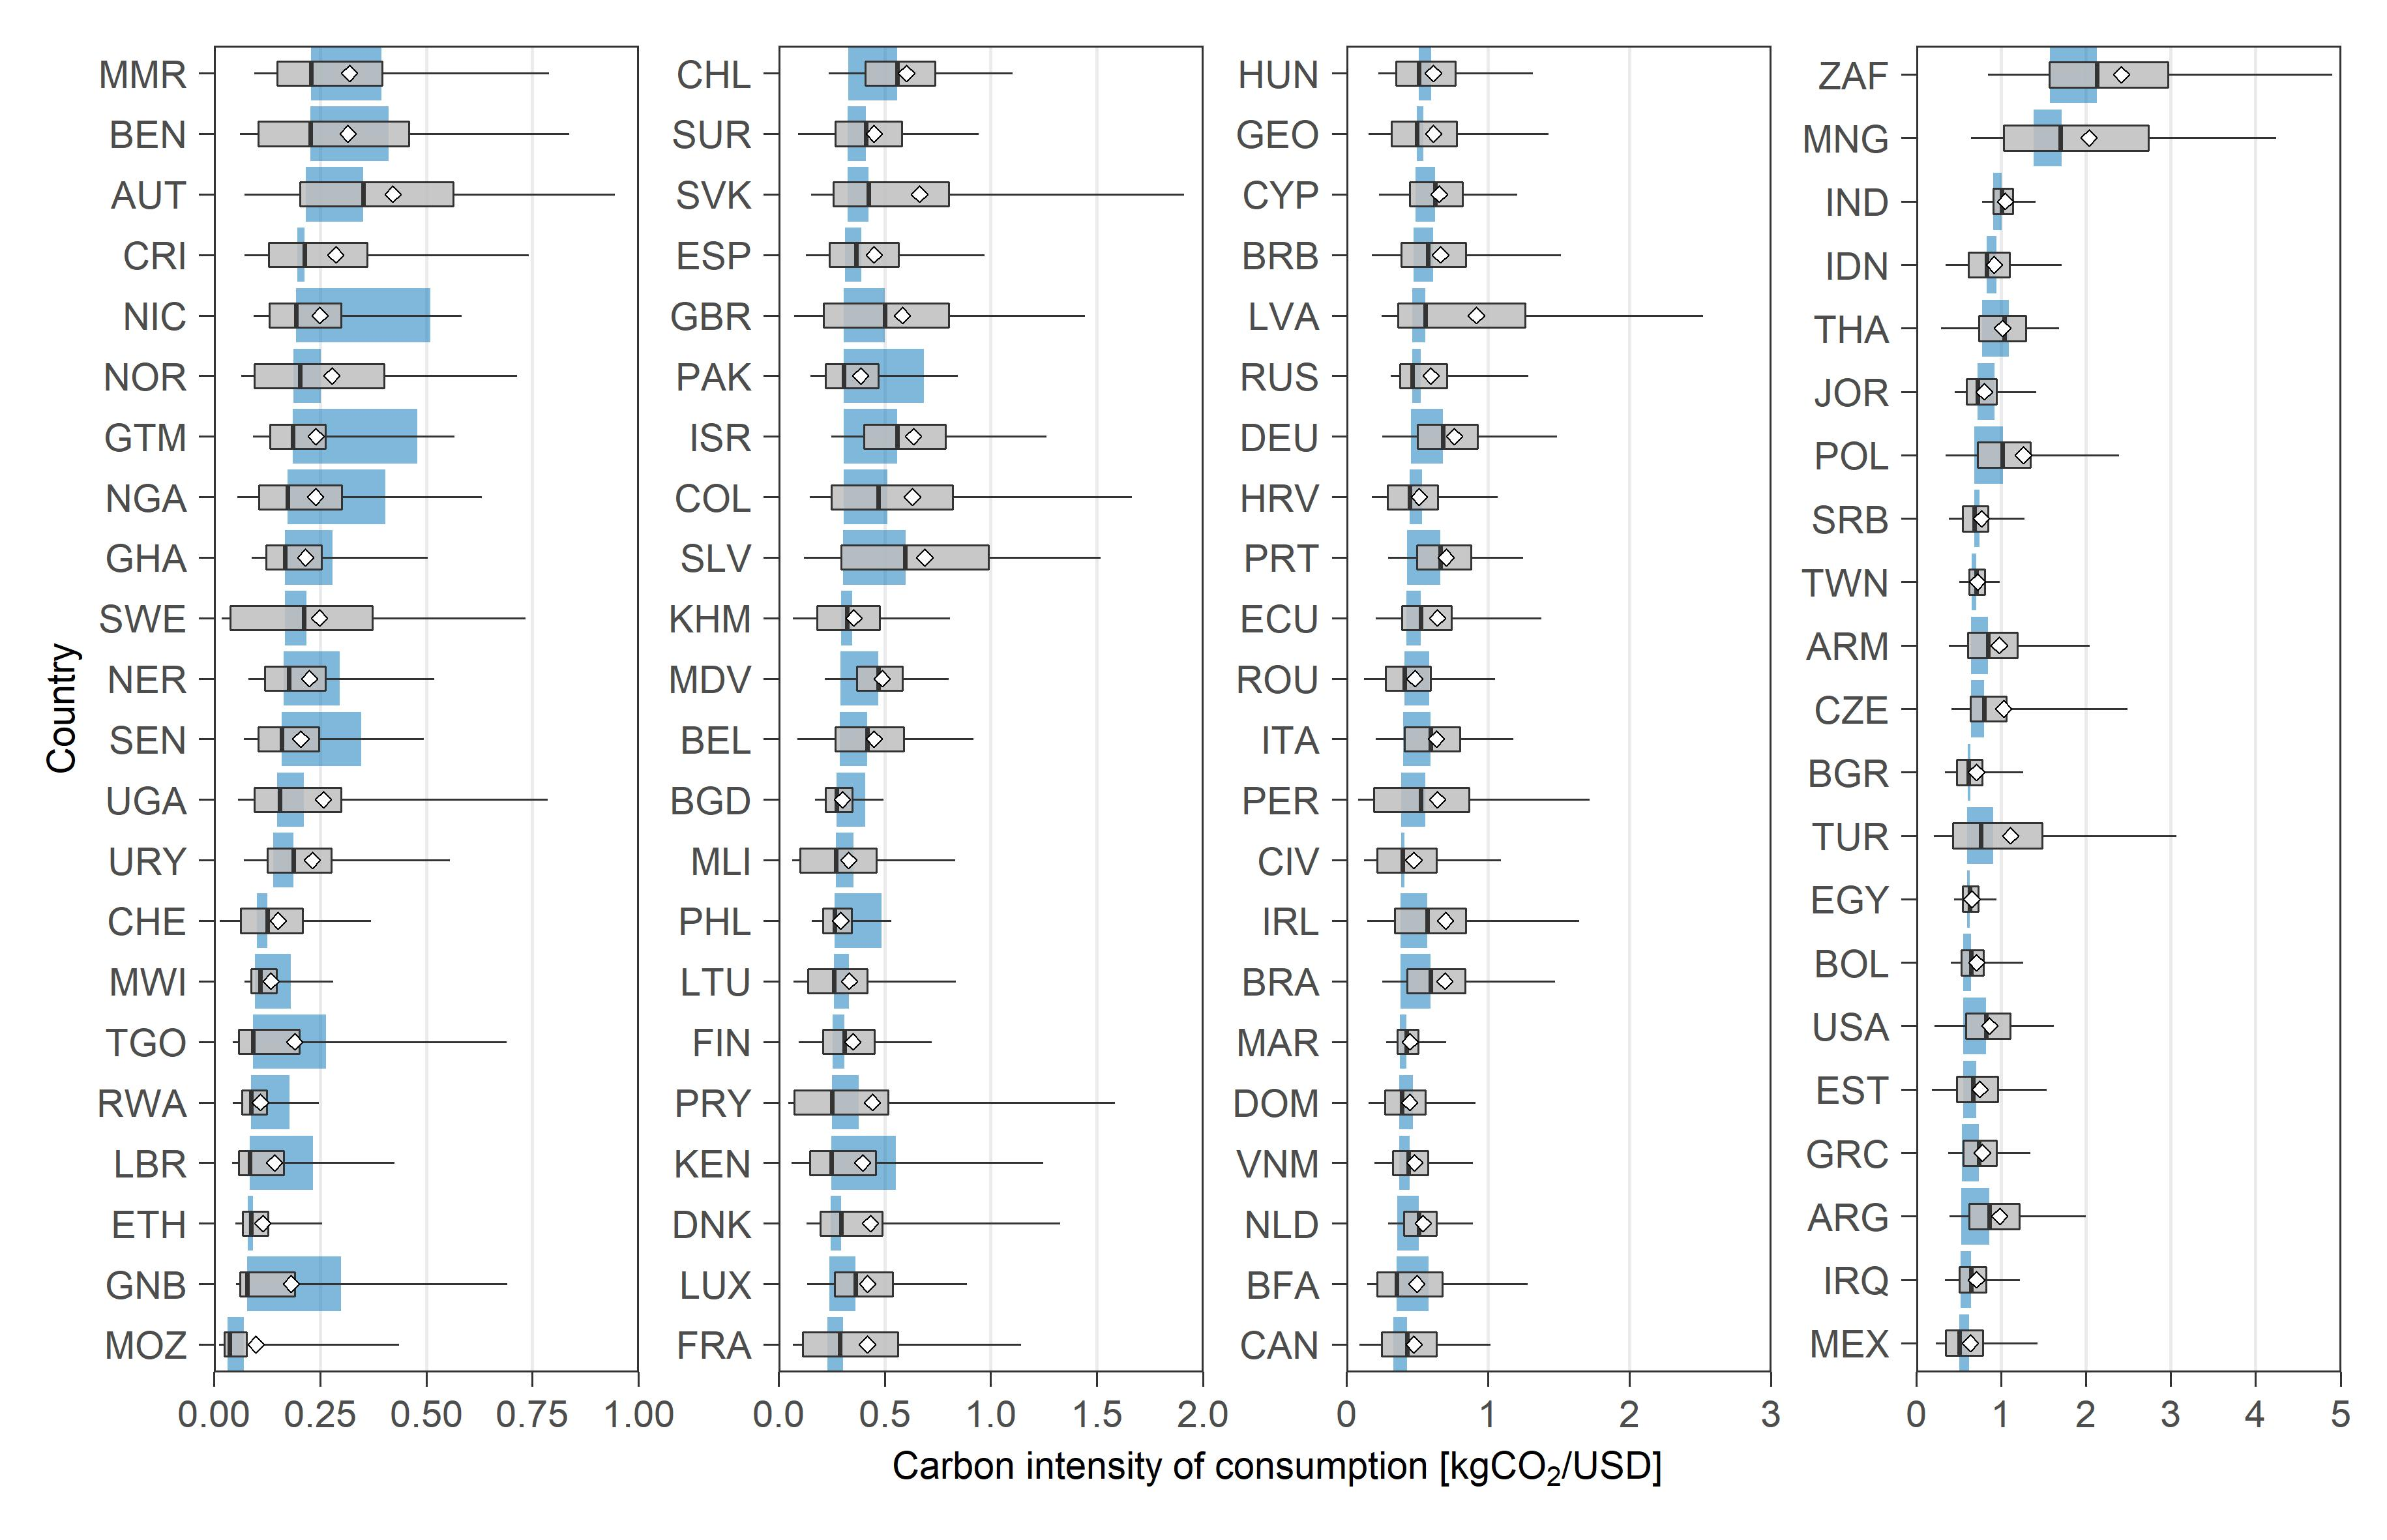
\includegraphics{Figure 1/Figure_1}
    \caption{Vertical differences and distribution of carbon intensity within poorest quintiles}
    \label{fig:fig_1}
    \begin{subcaption}
    Boxplots display the distribution of household-level carbon intensity within the poorest quintile in each of 87 countries: The boxes display the $25^{th}$ and $75^{th}$ percentile; whiskers display the $5^{th}$ and $95^{th}$ percentile, respectively. Rhombuses display the mean. Blue bars represent the vertical difference in household-level carbon intensity, i.e., the difference between the highest and the lowest median carbon intensity across quintiles.
    \end{subcaption}
\end{figure}

Figure \ref{fig:fig_1} illustrates that within-quintile heterogeneity exceeds between-quintile differences in \textit{all} countries \footnote{See FIGURE REF MISSING for country-level comparisons across all expenditure quintiles}. This underlines that analysis building on differences in income to explain differences in carbon intensity of consumption (or the impact of climate policy) might be insufficient since it falls short of accounting for differences in carbon intensity at similar levels of income. Instead, we propose including household-level characteristics beyond income in such an analysis to paint a more nuanced picture of which households' consumption is especially carbon-intensive.

This is also warranted, because - as we show in Figure \ref{fig:fig_2} - within-quintile differences are different across quintiles. To facilitate comparison across countries, we compute two coefficients \autocite{Missbach.2023b}: The vertical distribution coefficient $\overline{V_{r}}$ compares median carbon intensity of the poorest and the richest expenditure quintile:

\begin{equation}
    \widehat{V_{r}} = \frac{\overline{e_{EQ1}}}{\overline{e_{EQ5}}}
\end{equation}

If median carbon intensity among poorer households exceeds (is smaller than) the median carbon intensity of richer households, $\widehat{V_{r}}>1$ ($\widehat{V_{r}}<1$) and climate policy would likely lead to \textit{regressive} (\textit{progressive}) outcomes.

The horizontal distribution coefficient $\overline{H_{r}}$ compares within-quintile differences of the poorest and the richest expenditure quintile:

\begin{equation}
    \widehat{H_{r}} = \frac{e_{EQ1}^{95} - e_{EQ1}^{5}}{e_{EQ5}^{95} - e_{EQ5}^{5}}
\end{equation}

$\widehat{H_{r}}>1$ ($\widehat{H_{r}}<1$) would indicate that within-quintile differences are larger (smaller) among poorer compared to richer households.

Figure \ref{fig:fig_2} illustrates that the average carbon intensity of consumption is larger among the poorest quintile in 52 out of 87 countries compared to the richest quintile. These countries have a higher GDP per capita than others: We observe $\widehat{V_{r}}>1$ for 25 out of 25 countries in our sample with the highest GDP per capita. In these countries, climate policies (such as carbon pricing) are likely to have regressive effects. Similarly, carbon intensity is higher for richer quintiles compared to poorer quintiles ($\widehat{V_{r}}>1$ ) in 21 out of 25 countries in our sample with the lowest GDP per capita. This is in line with inverse-U-shaped Engel curves for carbon-intensive goods and services across countries and income quintiles \autocite{Dorband.2019}. %Interestingly, this does not necessarily hold in each single country.

\begin{figure}[ht!]
    \centering
    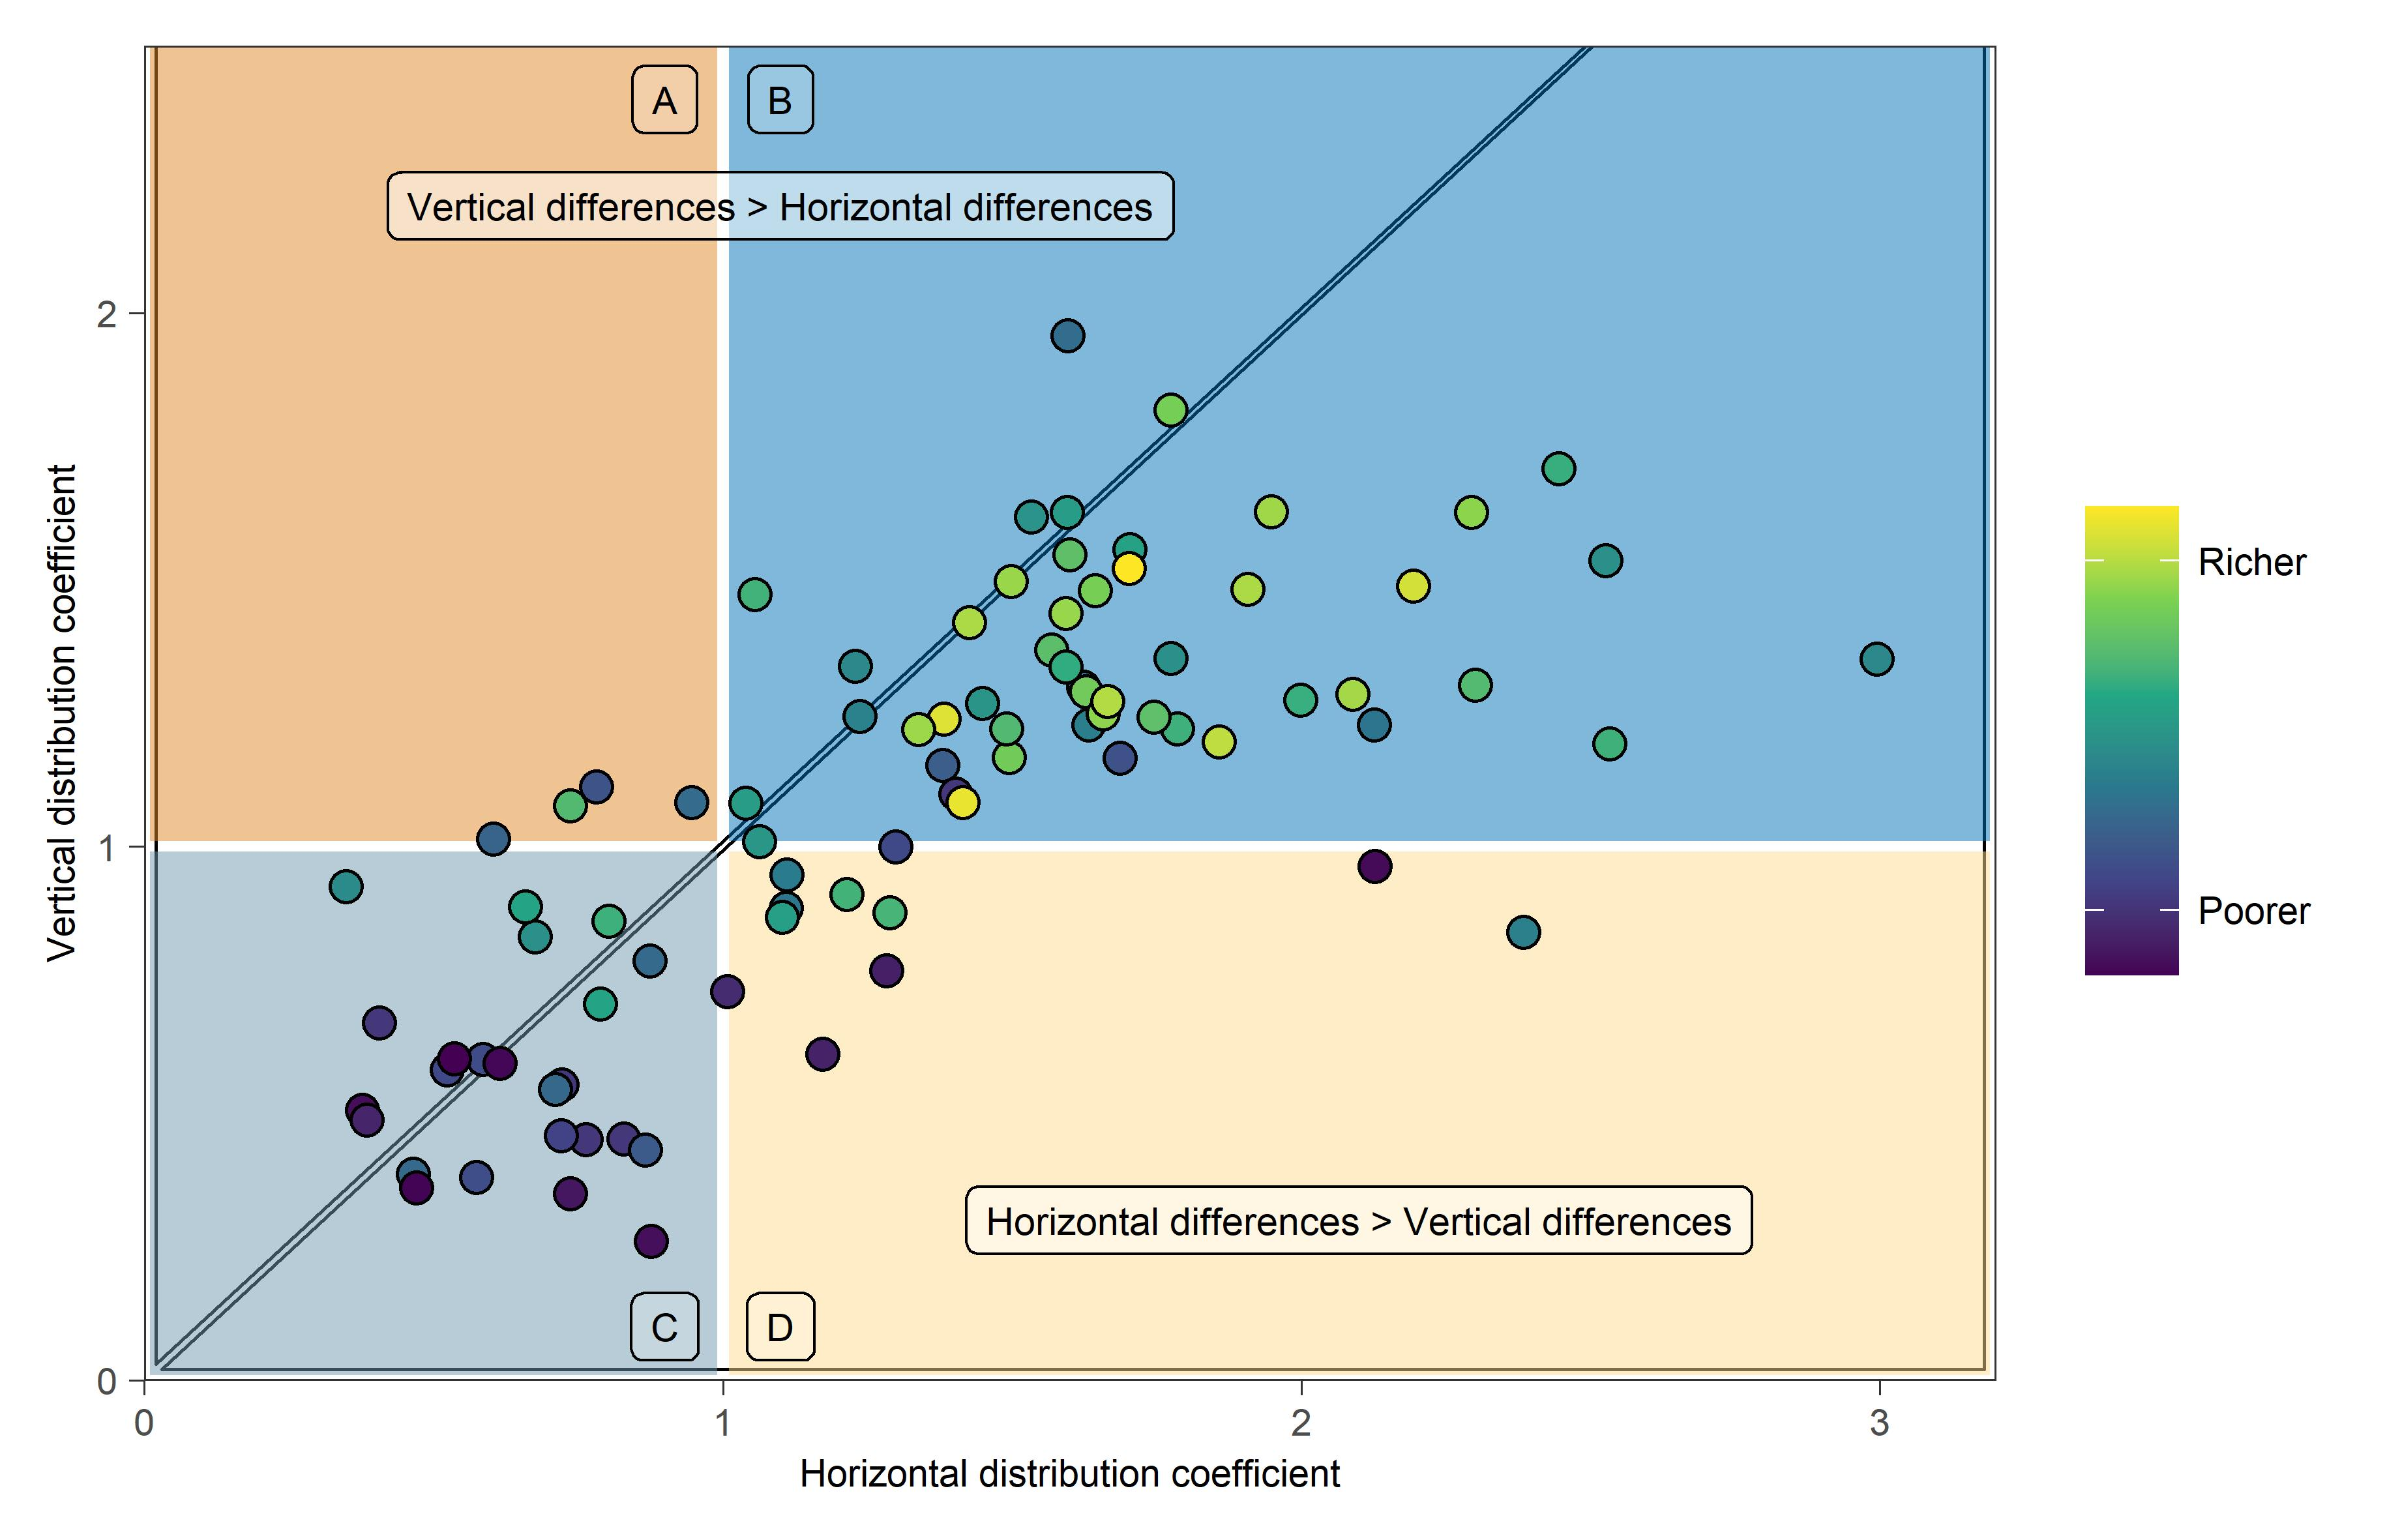
\includegraphics{Figure 2/Figure_2}
    \caption{Vertical and horizontal distribution coefficient}
    \label{fig:fig_2}
    \begin{subcaption}
    The vertical distribution coefficient compares the median carbon intensity of the richest to the poorest quintile. The horizontal distribution coefficient compares the within-quintile differences ($5^{th}$ to $95_{th}$ percentile within quintiles) of the richest to the poorest quintile. Rectangles (A) and (B) indicate higher carbon intensity (at the median) among the poorest quintile compared to the richest quintile; rectangles (C) and (D) indicate lower carbon intensity (at the median) among the poorest quintile compared to the richest quintile. Rectangles (A) and (C) indicate smaller within-quintile differences of carbon intensity among the richest quintile compared to the poorest quintile; rectangles (B) and (D) indicate larger within-quintile differences of carbon intensity among the richest quintile compared to the poorest quintile. Colors of points indicate GDP per capita for 2018 (in log-transformed constant 2010 US-\$). See also Table \ref{tab:A7}.
    \end{subcaption}
\end{figure}

In 59 out of 87 countries, within-quintile variation (expressed as the difference between the $5^{th}$ and the $95^{th}$ quantile within quintiles) is larger in the poorest quintile compared to the richest quintile. Horizontal differences, i.e., within-quintile heterogeneity, exceeds vertical differences, i.e., between-quintile heterogeneity in 65 countries, emphasizing the need for detailed investigation of household characteristics associated to higher levels of carbon intensity of consumption.

In response, one core assumption of this study is that $e_{i}$, the carbon intensity of household \textit{i}, correlates with observable household characteristics $X_{i}^{'}$:

\begin{equation}
    e_{i} \sim X_{i}^{'}
\end{equation}

% Which criteria should be included in modelling and why?
% Discuss main arguments for single characteristics (possibly already in methods section).

We analyze which household characteristics are associated to higher levels of carbon intensity of consumption with the help of two modeling approaches, namely boosted regression trees (BRT) and a logit-model.

\paragraph{Boosted regression trees} Fitting boosted regression trees (BRT) \autocite{Friedman.2003, Elith.2008} is a supervised machine learning method allowing for detection of non-linear relationships and interaction effects between an outcome and many predictor variables (features). As an extension to regression trees, the BRT algorithm (\textit{XGBoost} \autocite{Chen.2016}) fits many single regression trees, iteratively giving higher weights to observations with larger predicting errors. This leads to large predictive power, also if compared to the frequently used random forest algorithm. Nevertheless, fitting BRT is usually more computationally intensive and outcomes are more difficult to interpret. % Why BRT is helpful here.

Deploying BRT serves the purpose of our analysis, because it is a priori ambiguous which variables to include in a model. Specifically, research indicates that the impacts of climate policy (and therefore the carbon intensity of consumption) distribute non-linearly across households with different characteristics, such as income, demographic groups \autocite{Missbach.2023}, energy use (cite MISSBACH LAC, Farrell) and space \autocite{Chan.2023}. Compared to other approaches, such as variance-based inequality decomposition \autocite{Farrell.2017,Sager.2019b,Missbach.2023b}, using BRT is well-suited to help identifying important predictors while also allowing detection of potentially non-linear relationships.

We build BRT-models on the country-level to investigate characteristics associated to heterogeneous levels of carbon intensities within single countries. The carbon intensity $e_{i}$ is the outcome variable. For each country-level model we use the entire set of observable household-level characteristics $X_{i}^{'}$ as possible features and perform several feature engineering steps (see also Appendix \ref{sec:featureengineering}).

The predictive performance of BRT-models critically hinges on several hyperparameters. For hyperparameter tuning, we randomly split country-level data into a training and a test sample, comprising 75\% and 25\% of observations, respectively. We use five-fold cross-validation on the training dataset to fit 1,000 trees - following the recommendations by \textcite{Elith.2008} - along with 16 different combinations of learning rate ($\eta \in [0.001,0.3]$, the maximum depth of trees (\textit{max\_depth} $\in \{x \in \mathbb{N} \mid 1  \leq x \leq 15 \}$) and a fraction of possible features included in each tree (\textit{mtry} $\in \{0.5,0.7,1\}$). For each country, we select the combination of hyperparamters that minimizes mean absolute error.

Building on selected hyperparameters, we use five-fold cross-validation on all observations, i.e., from the training and test set, for model evaluation. We evaluate model performance with the help of mean absolute error (MAE), root mean squared error (RMSE) and $R^{2}$. We also use all observations to evaluate the relative importance of each feature with the help of SHAP-values \autocite{Lundberg.2020}: SHAP-values represent the contribution of each feature to each individual prediction. Shap-values have recently been established as a more suitable means to interpret outcomes of machine learning models compared to other approaches. We also determine feature importance by calculating the average absolute SHAP-value for each feature across all individual predictions. We show feature importance as a share of contribution (in \% of total mean absolute SHAP-values) to allow for better comparability of feature importance across countries. We visualize the distribution of SHAP-values for the most important features in each country over feature values, i.e., partial dependence plots. 

\paragraph{Logit-model} We also fit a logit-model to identify households whose consumption is relatively carbon-intensive compared to the entire population. We construct a binary variable $e_{i}^{80}$ for each household \textit{i} indicating whether the household is among the most carbon-intensive 20\% of households in each country:

\begin{equation}
    e_{i}^{80} =
    \begin{cases}
    1, & \text{for }  e_{i} \geq e^{80} \\
    0, & \text{for }  e_{i} < e^{80}
    \end{cases}
\end{equation}

Subsequently, be $P_{e_{i}^{80}}$ the probability of household \textit{i} to consume more carbon-intensively than 80\% of the population in each country. We are interested in the coefficients $\beta^{'}$ of the following logit-model:

\begin{equation}
    log \left( \frac{P_{e_{i}^{80}}}{1 - P_{e_{i}^{80}}} \right) = \alpha_{0} + \beta^{'} X_{i}^{'} + \varepsilon_{i}
\end{equation}

Estimating a logit-model serves as a robustness check for results from BRT-models. It also allows for investigation of characteristics associated to "hardship-case" households including a more accessible interpretation of results and parameters. We show results from logit-models with the help of regression tables and visualize average marginal effects for each independent variable.

\paragraph{Clustering} Country-level analyses can be meaningful to identify country-specific household characteristics associated to higher levels of carbon intensity of consumption. In fact, the relationship between household-level characteristics and carbon intensity of consumption is unique for each country, but also contingent on availability of granular data. To account for differences in available features across countries, we correct individual feature importance by multiplying individual feature importance and $R^{2}$. This approach also helps to account for the aggregate performance of the model and allows for better comparison of country-level model performance.

Building on (adjusted) feature importance for each country we use k-means clustering algorithm to learn more about which characteristics are more important in many countries. If features are missing in the data, we assume its share of contribution is zero. We normalize all variables to allow for comparison across variables. If one feature is more (less) important in one country compared to all other countries, the processed feature value will be relatively high (low). If one feature is equally important across all countries, processed feature values will be close to zero.

K-means clustering is an unsupervised machine-learning method and helps to analyze clusters of observations which are most similar in many variables within each cluster and least similar in many variables across clusters \autocite{MacQueen.1967}. We inspect the optimal number of clusters with the help of average silhouette widths \autocite{Rousseeuw.1987} for each cluster \textit{k}. The silhouette width $s_{i}$ accounts for the average distance of each observation \textit{i} to all other observations within its cluster and for the average distance to observations from the nearest neighbouring cluster. Silhouettes closer to $1$ indicate a good fit of an observation to its cluster and silhouettes closer to $-1$ indicate a poor fit. The average silhouette width $\overline{s_{k}}$ for each cluster \textit{k} expresses how well all observations fit on average to each cluster. Our approach yields $k = 14$ to be the number of clusters maximizing average silhouette width\footnote{See Figures\ref{fig:G1_silhouette} and \ref{fig:G2_silhouette} for visualization.}.

For each country-cluster, we compute average values for each feature to allow for investigation of differences between countries in different clusters. We also investigate which country is most likely to all other countries in each cluster maximizing silhouette width within each cluster and use it to demonstrate cluster-level characteristics. It is important to note that our approach to adjust feature values for total model performance reduces in the influence of feature availability in the data for clustering. Uncorrected feature importance values may be exaggerated, if only few features exist, so countries with few features may end up in wrong clusters simply because the model cannot help explain much of the variation in carbon intensity. Instead, our approach ensures that all \textit{observable} features contribute to clustering. Despite many structurally unobservable household-level features, our approach might be warranted under the assumption that policy formulation (for example on optimal targeting of compensation measures) can naturally only center on observable characteristics, if targeting errors should be minimized.

\begin{itemize}
    \item Methodological discussion (brief)
    %\item Analyzing vertical inequality
    %\item Analyzing horizontal inequality
    %\item Introduce boosted regression trees
    %\item Introduce logit model as robustness check, supplementary analysis
    \item Critical appraisal
\end{itemize}

\clearpage

\section{Results: Heterogeneity of carbon intensity of consumption} \label{sec:results}

Building on model outcomes to help identifying factors associated to higher levels of carbon intensity of consumption, we cluster countries which are similar to each other, i.e., in which features are similarly important for model prediction. Figure \ref{fig:fig_3} shows the relative importance of different features across country-clusters. 

%What are important criteria to assign countries to different clusters?

\paragraph{Country clusters}

The largest cluster comprises 14 countries (including USA, Germany and Italy)

\begin{figure}[ht!]
    \centering
    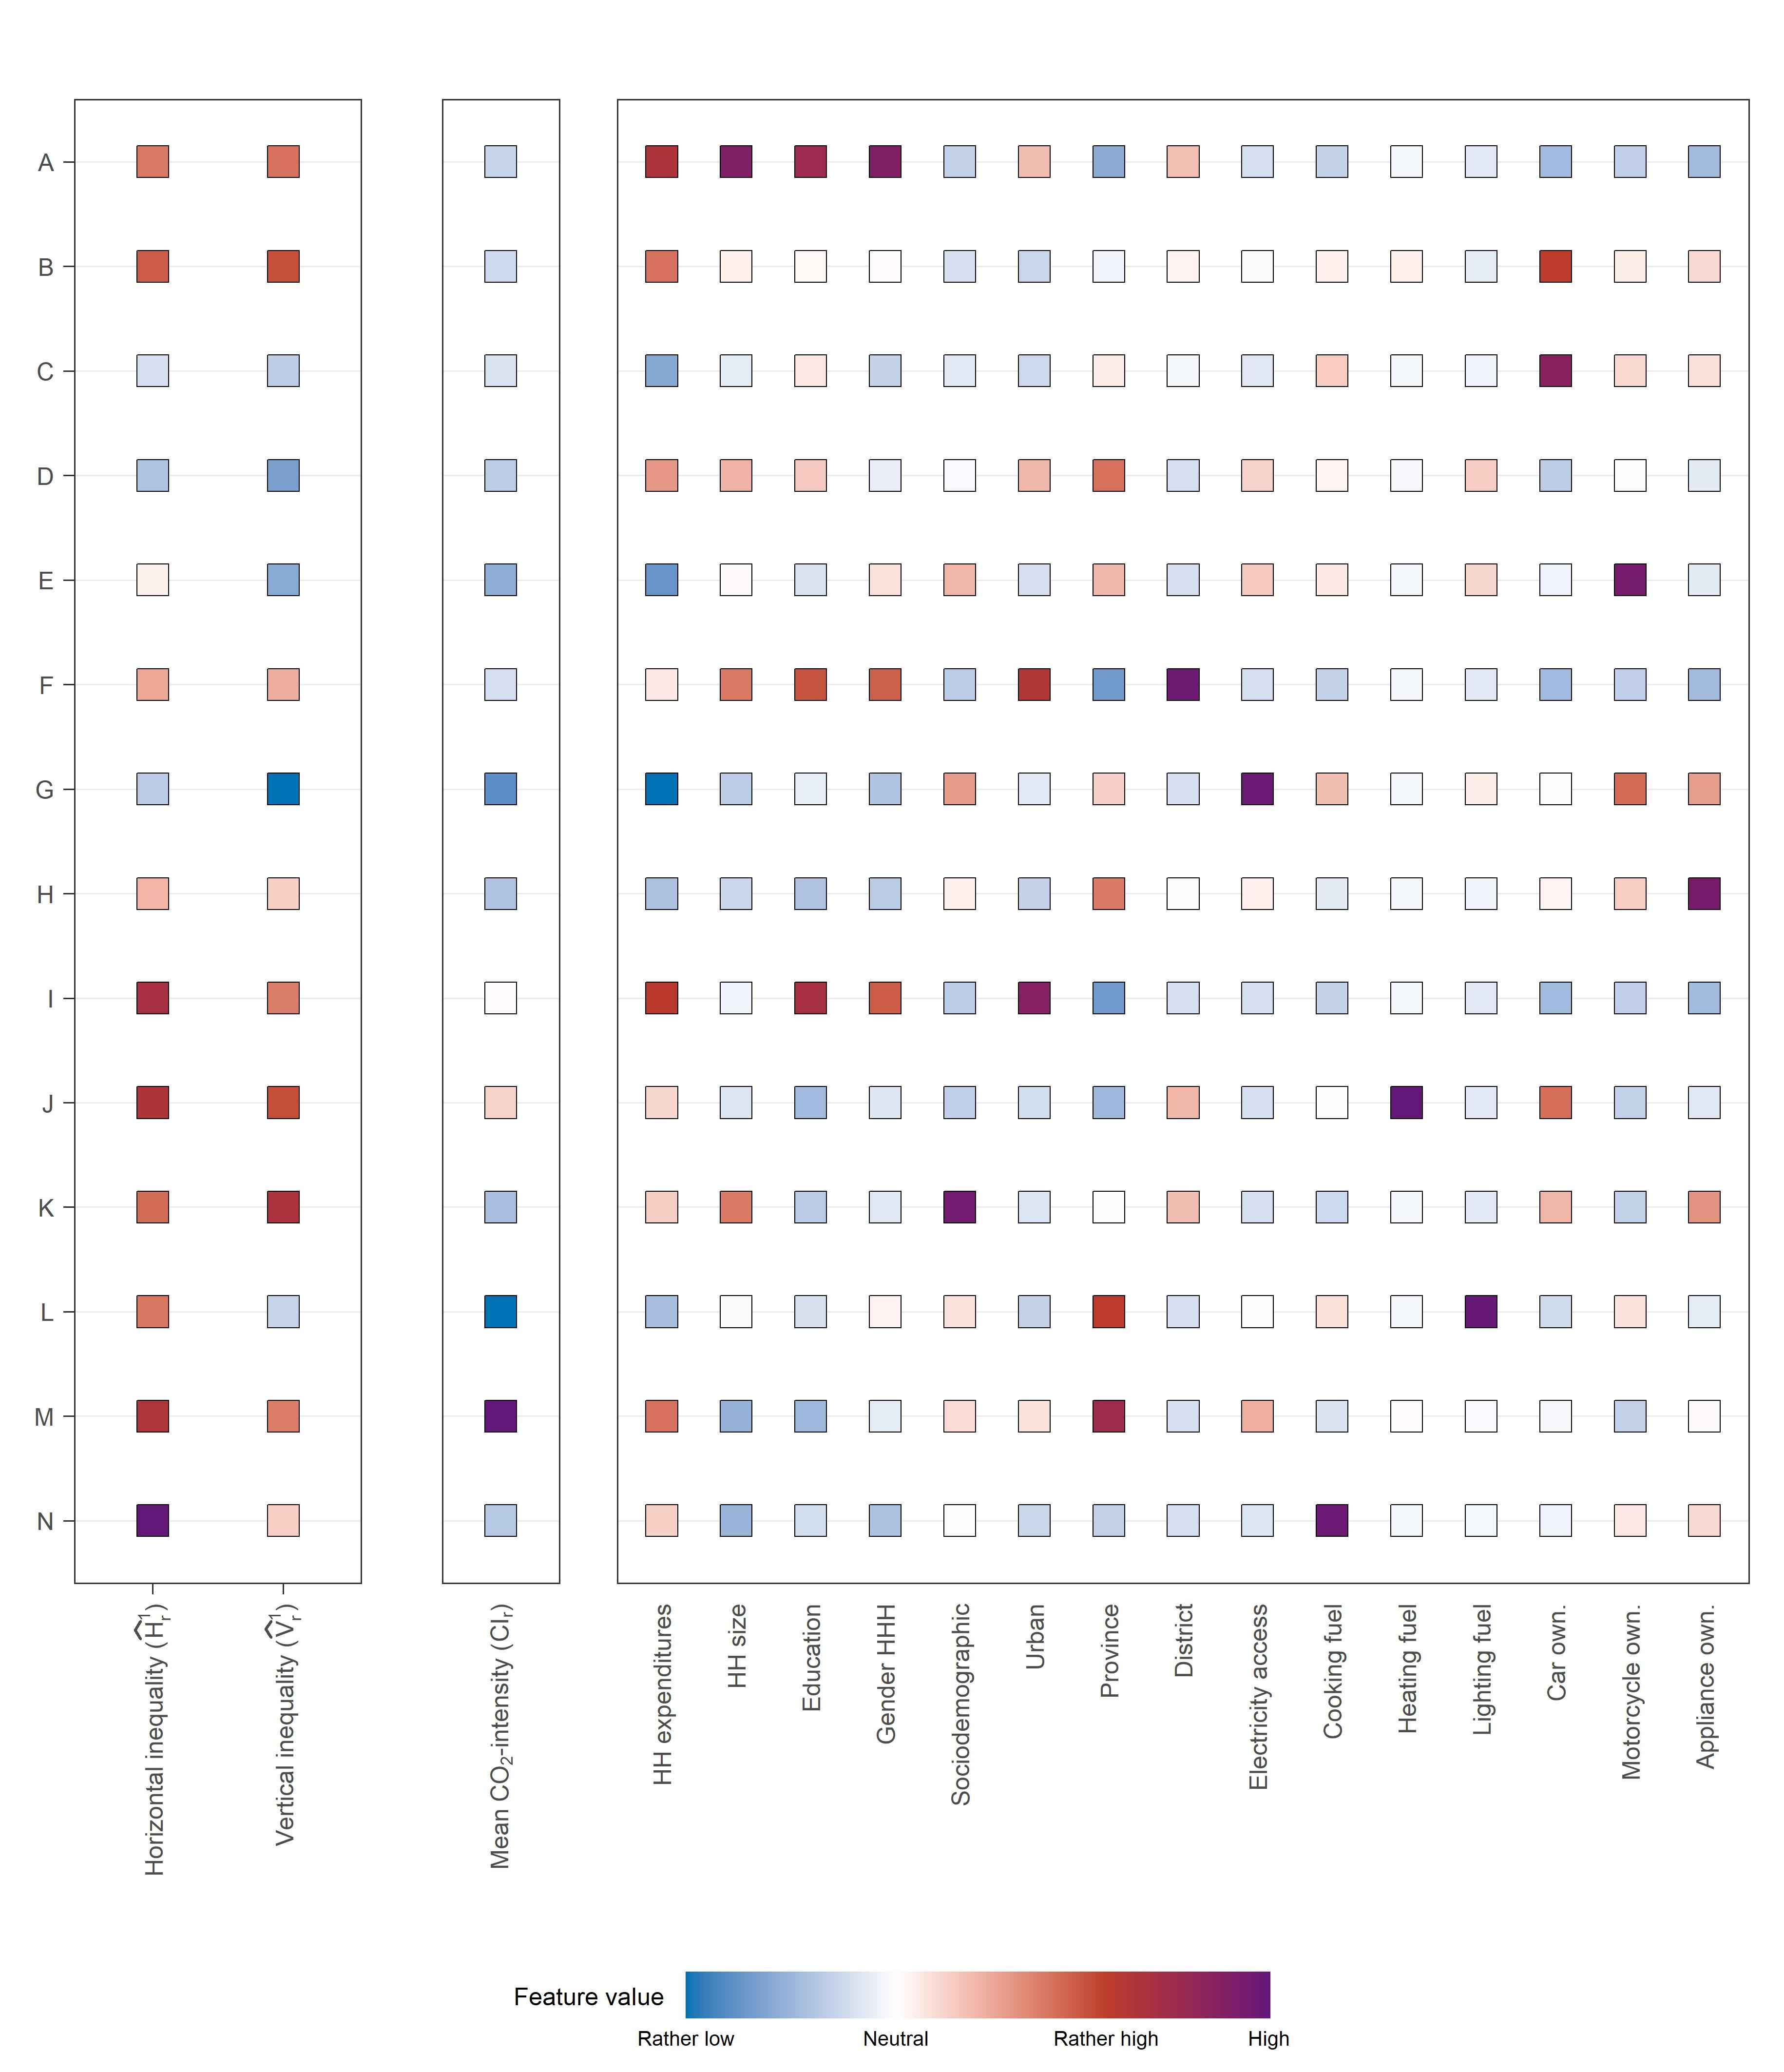
\includegraphics{Figure 3/Figure_3}
    \caption{Average feature importance across country clusters}
    \label{fig:fig_3}
    \begin{subcaption}
    This figure shows the average importance of features (in normalized absolute average SHAP-values) across all countries from each cluster A to N. Colors express the average importance of features in a cluster in comparison to other clusters. Blue (red) colors indicate that a feature is relatively less (more) important on average in a cluster compared to all other clusters. 'Sociodemographic' comprises normalized absolute average SHAP values for features such as ethnicity, nationality, religion or language.
    For horizontal inequality, blue (red) colors indicate a lower (higher) heterogeneity within the first income quintile compared to the fifth income quintile. For vertical inequality, blue (red) colors indicate lower (higher) median carbon intensity among the first income quintile compared to the fifth income quintile. For average $CO_{2}$-intensity, blue (red) colors indicate a lower (higher) average carbon intensity across clusters. We assign countries to 14 clusters performing k-means clustering. We also show all values in Table \ref{tab:A9}.
    \end{subcaption}
\end{figure}

\paragraph{Country-level feature importance}

Figures \ref{fig:fig_4_1} and \ref{fig:fig_4_2} show the relative importance of features for each country across clusters. %Describe single clusters, at least A, B, C and D. Touch briefly upon the rest.
% What are important features? In which direction? Why?

\begin{figure}[ht!]
    \centering
    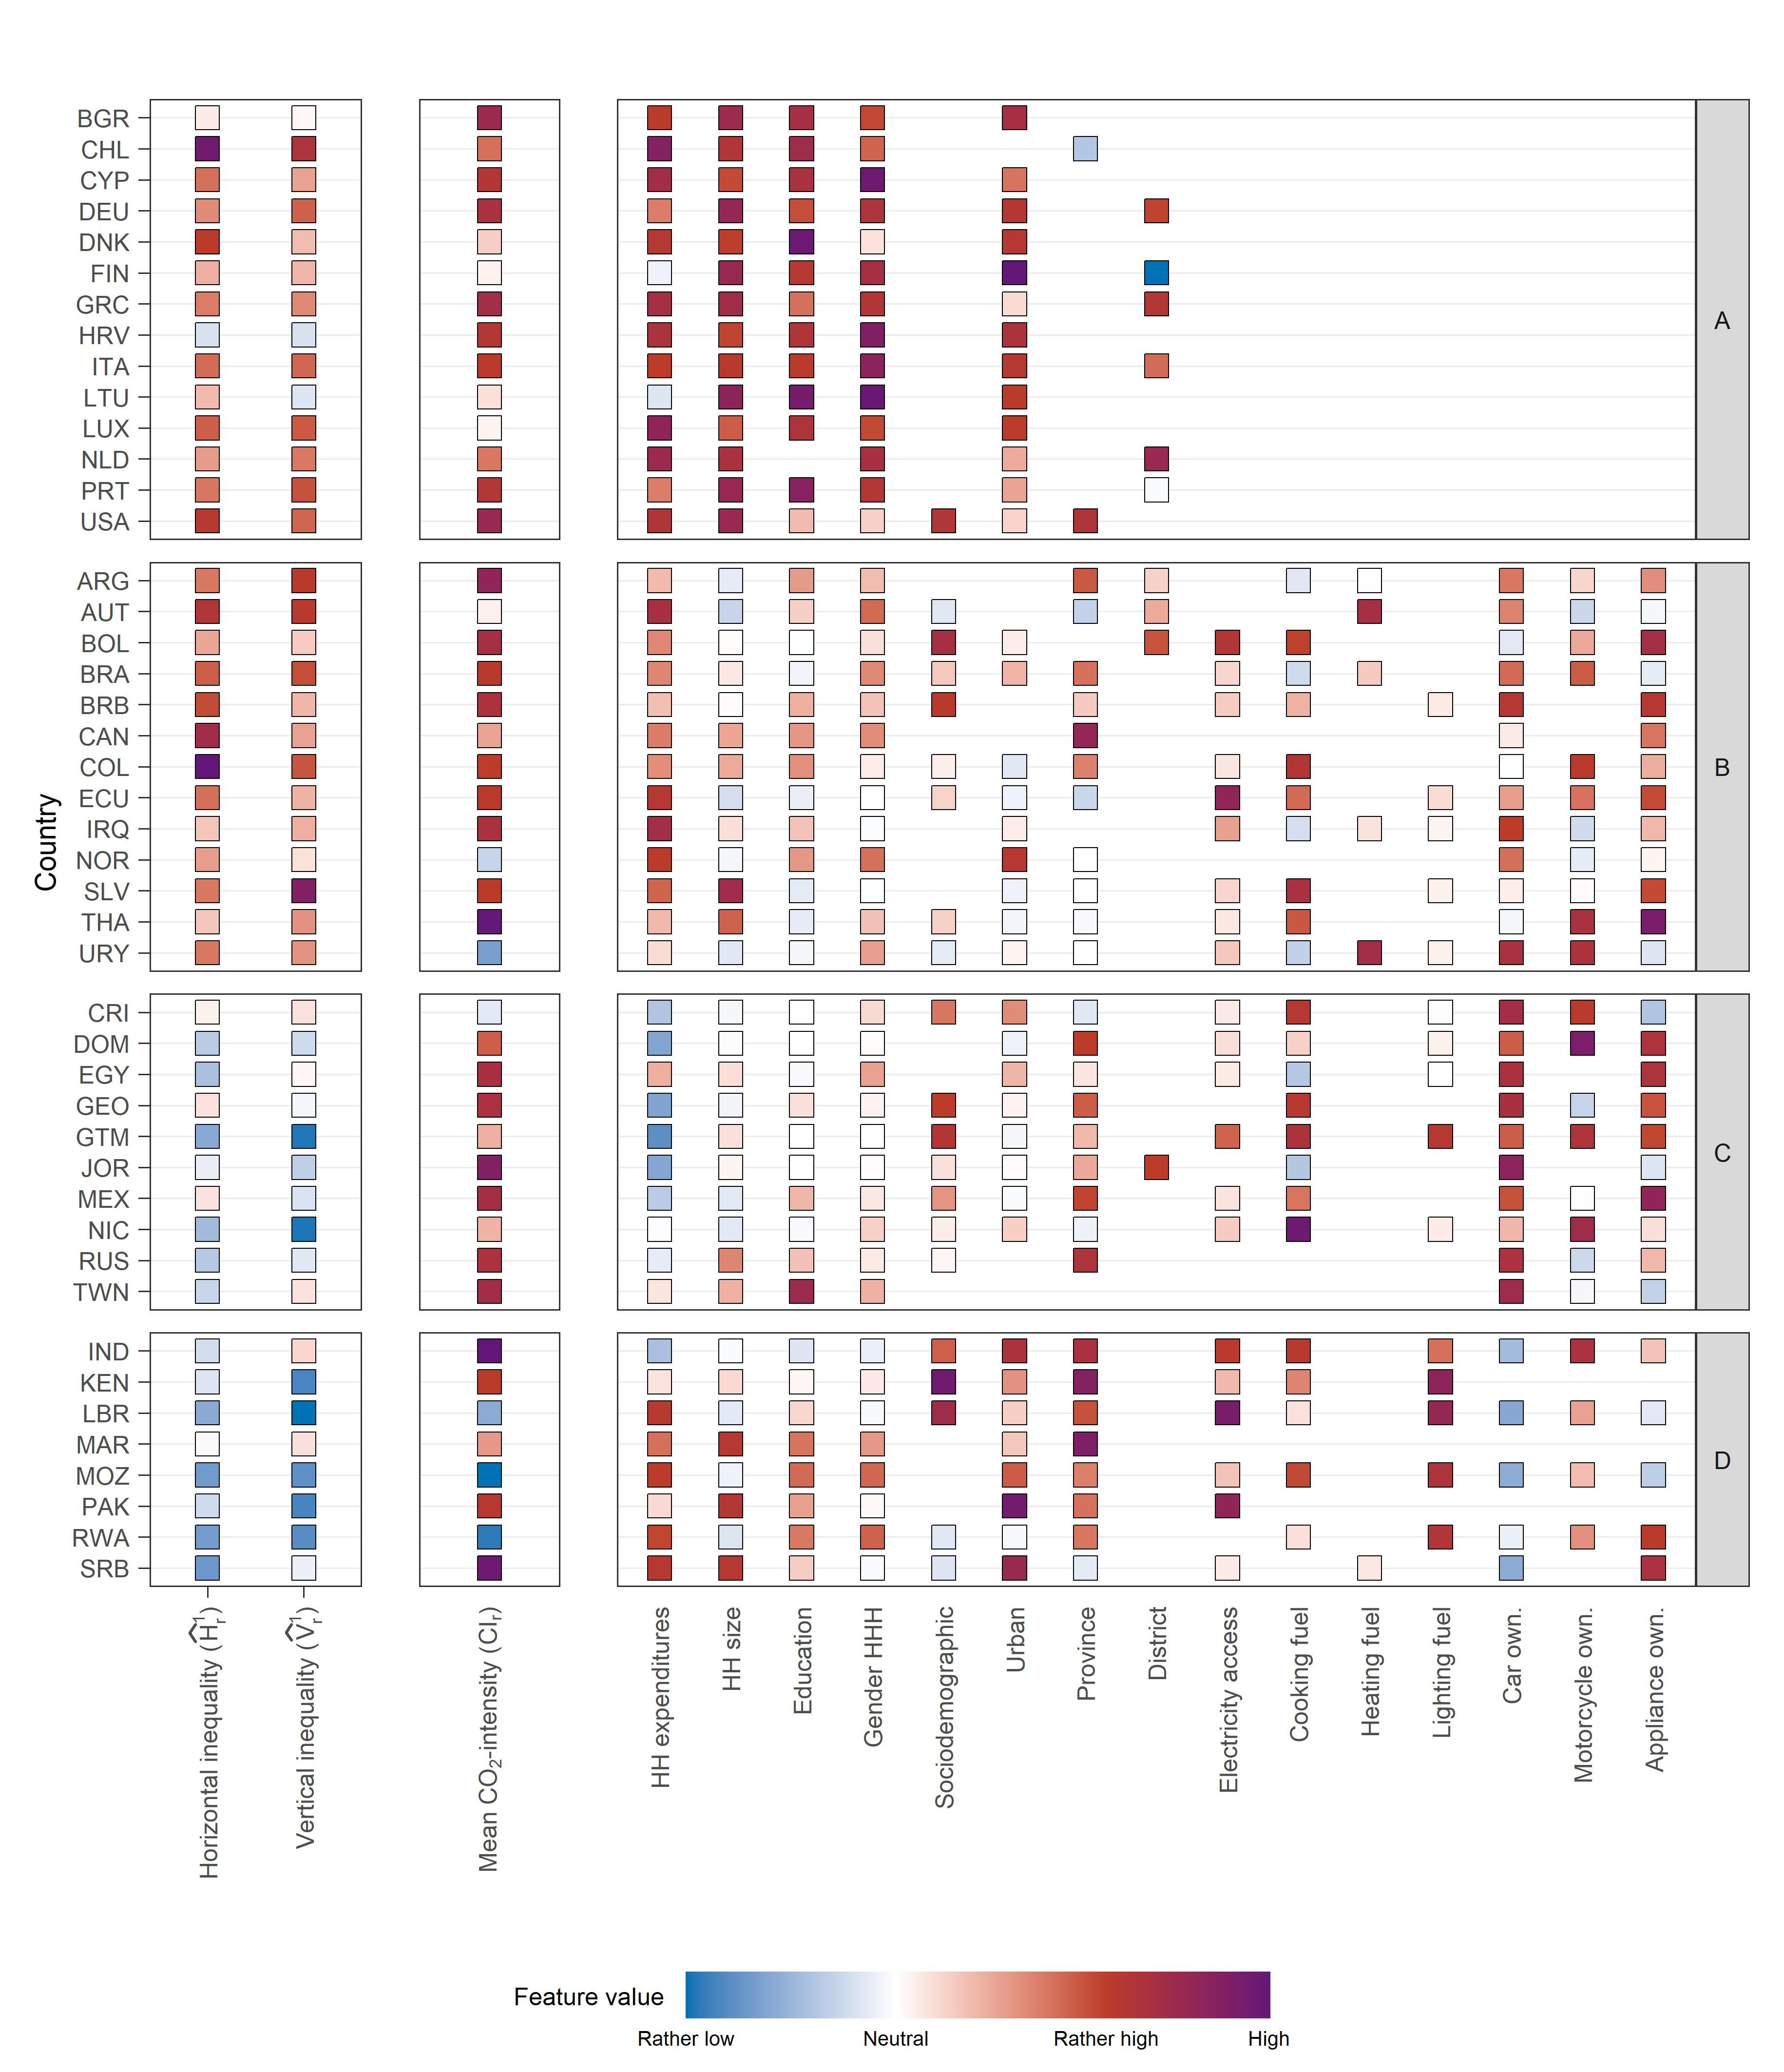
\includegraphics{Figure 4/Figure_4_1}
    \caption{Feature importance across countries by cluster}
    \label{fig:fig_4_1}
    \begin{subcaption}
    This figure shows the importance of features (in normalized average absolute SHAP-values) for each country, grouped by country clusters. Blue (red) colors indicate that a feature is relatively less (more) important in a country compared to all other countries. 'Sociodemographic' comprises normalized absolute SHAP-values for features such as ethnicity, nationality, religion or language.
    For horizontal inequality, blue (red) colors indicate a lower (higher) heterogeneity within the first income quintile compared to the fifth income quintile. For vertical inequality, blue (red) colors indicate lower (higher) median carbon intensity among the first income quintile compared to the fifth income quintile. For average $CO_{2}$-intensity, blue (red) colors indicate a lower (higher) average carbon intensity across all countries.
    We assign countries to 14 clusters performing k-means clustering based on scaled values across all features. We also show all values in Table \ref{tab:A10}.
    \end{subcaption}
\end{figure}

\begin{figure}[ht!]
    \centering
    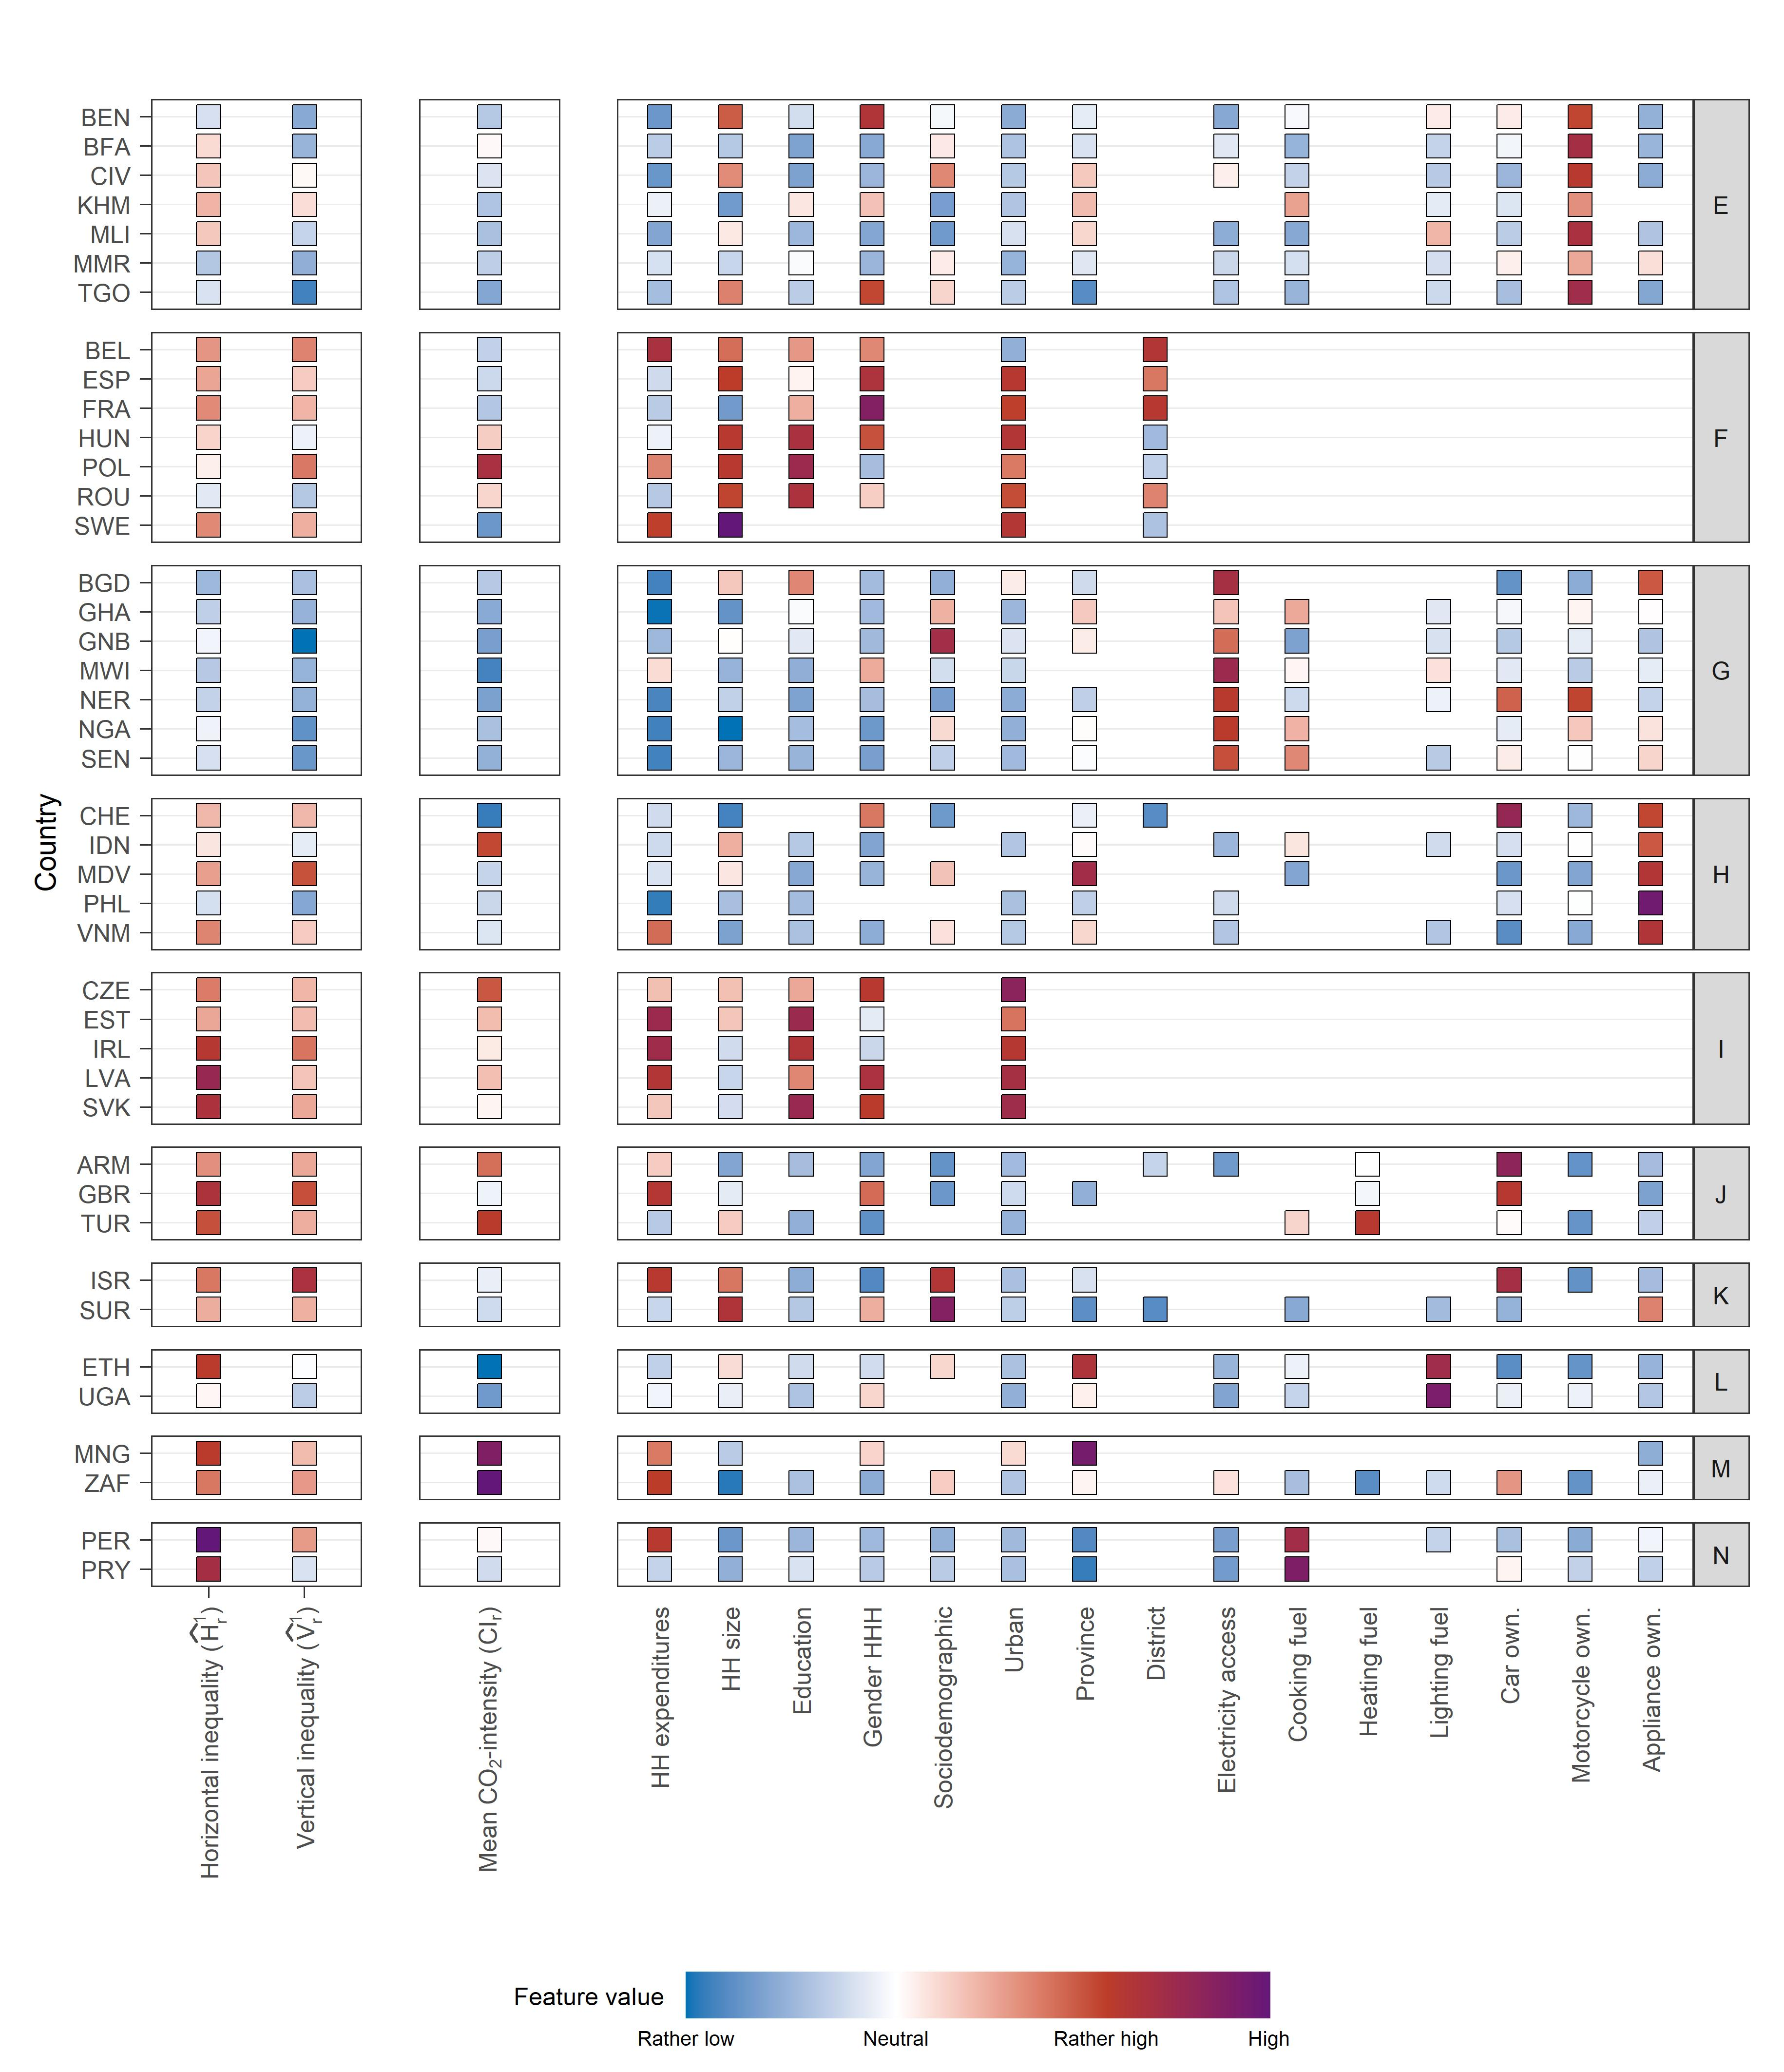
\includegraphics{Figure 4/Figure_4_2}
    \caption{Feature importance across countries by cluster}
    \label{fig:fig_4_2}
    \begin{subcaption}
    This figure shows the importance of features (in normalized average absolute SHAP-values) for each country, grouped by country clusters. Blue (red) colors indicate that a feature is relatively less (more) important in a country compared to all other countries. 'Sociodemographic' comprises normalized absolute SHAP-values for features such as ethnicity, nationality, religion or language.
    For horizontal inequality, blue (red) colors indicate a lower (higher) heterogeneity within the first income quintile compared to the fifth income quintile. For vertical inequality, blue (red) colors indicate lower (higher) median carbon intensity among the first income quintile compared to the fifth income quintile. For average $CO_{2}$-intensity, blue (red) colors indicate a lower (higher) average carbon intensity across all countries.
    We assign countries to 14 clusters performing k-means clustering based on scaled values across all features. We also show all values in Table \ref{tab:A10}.
    \end{subcaption}
\end{figure}

\paragraph{Household characteristics and heterogeneous carbon intensity of consumption}

\begin{figure}[ht!]
    \centering
    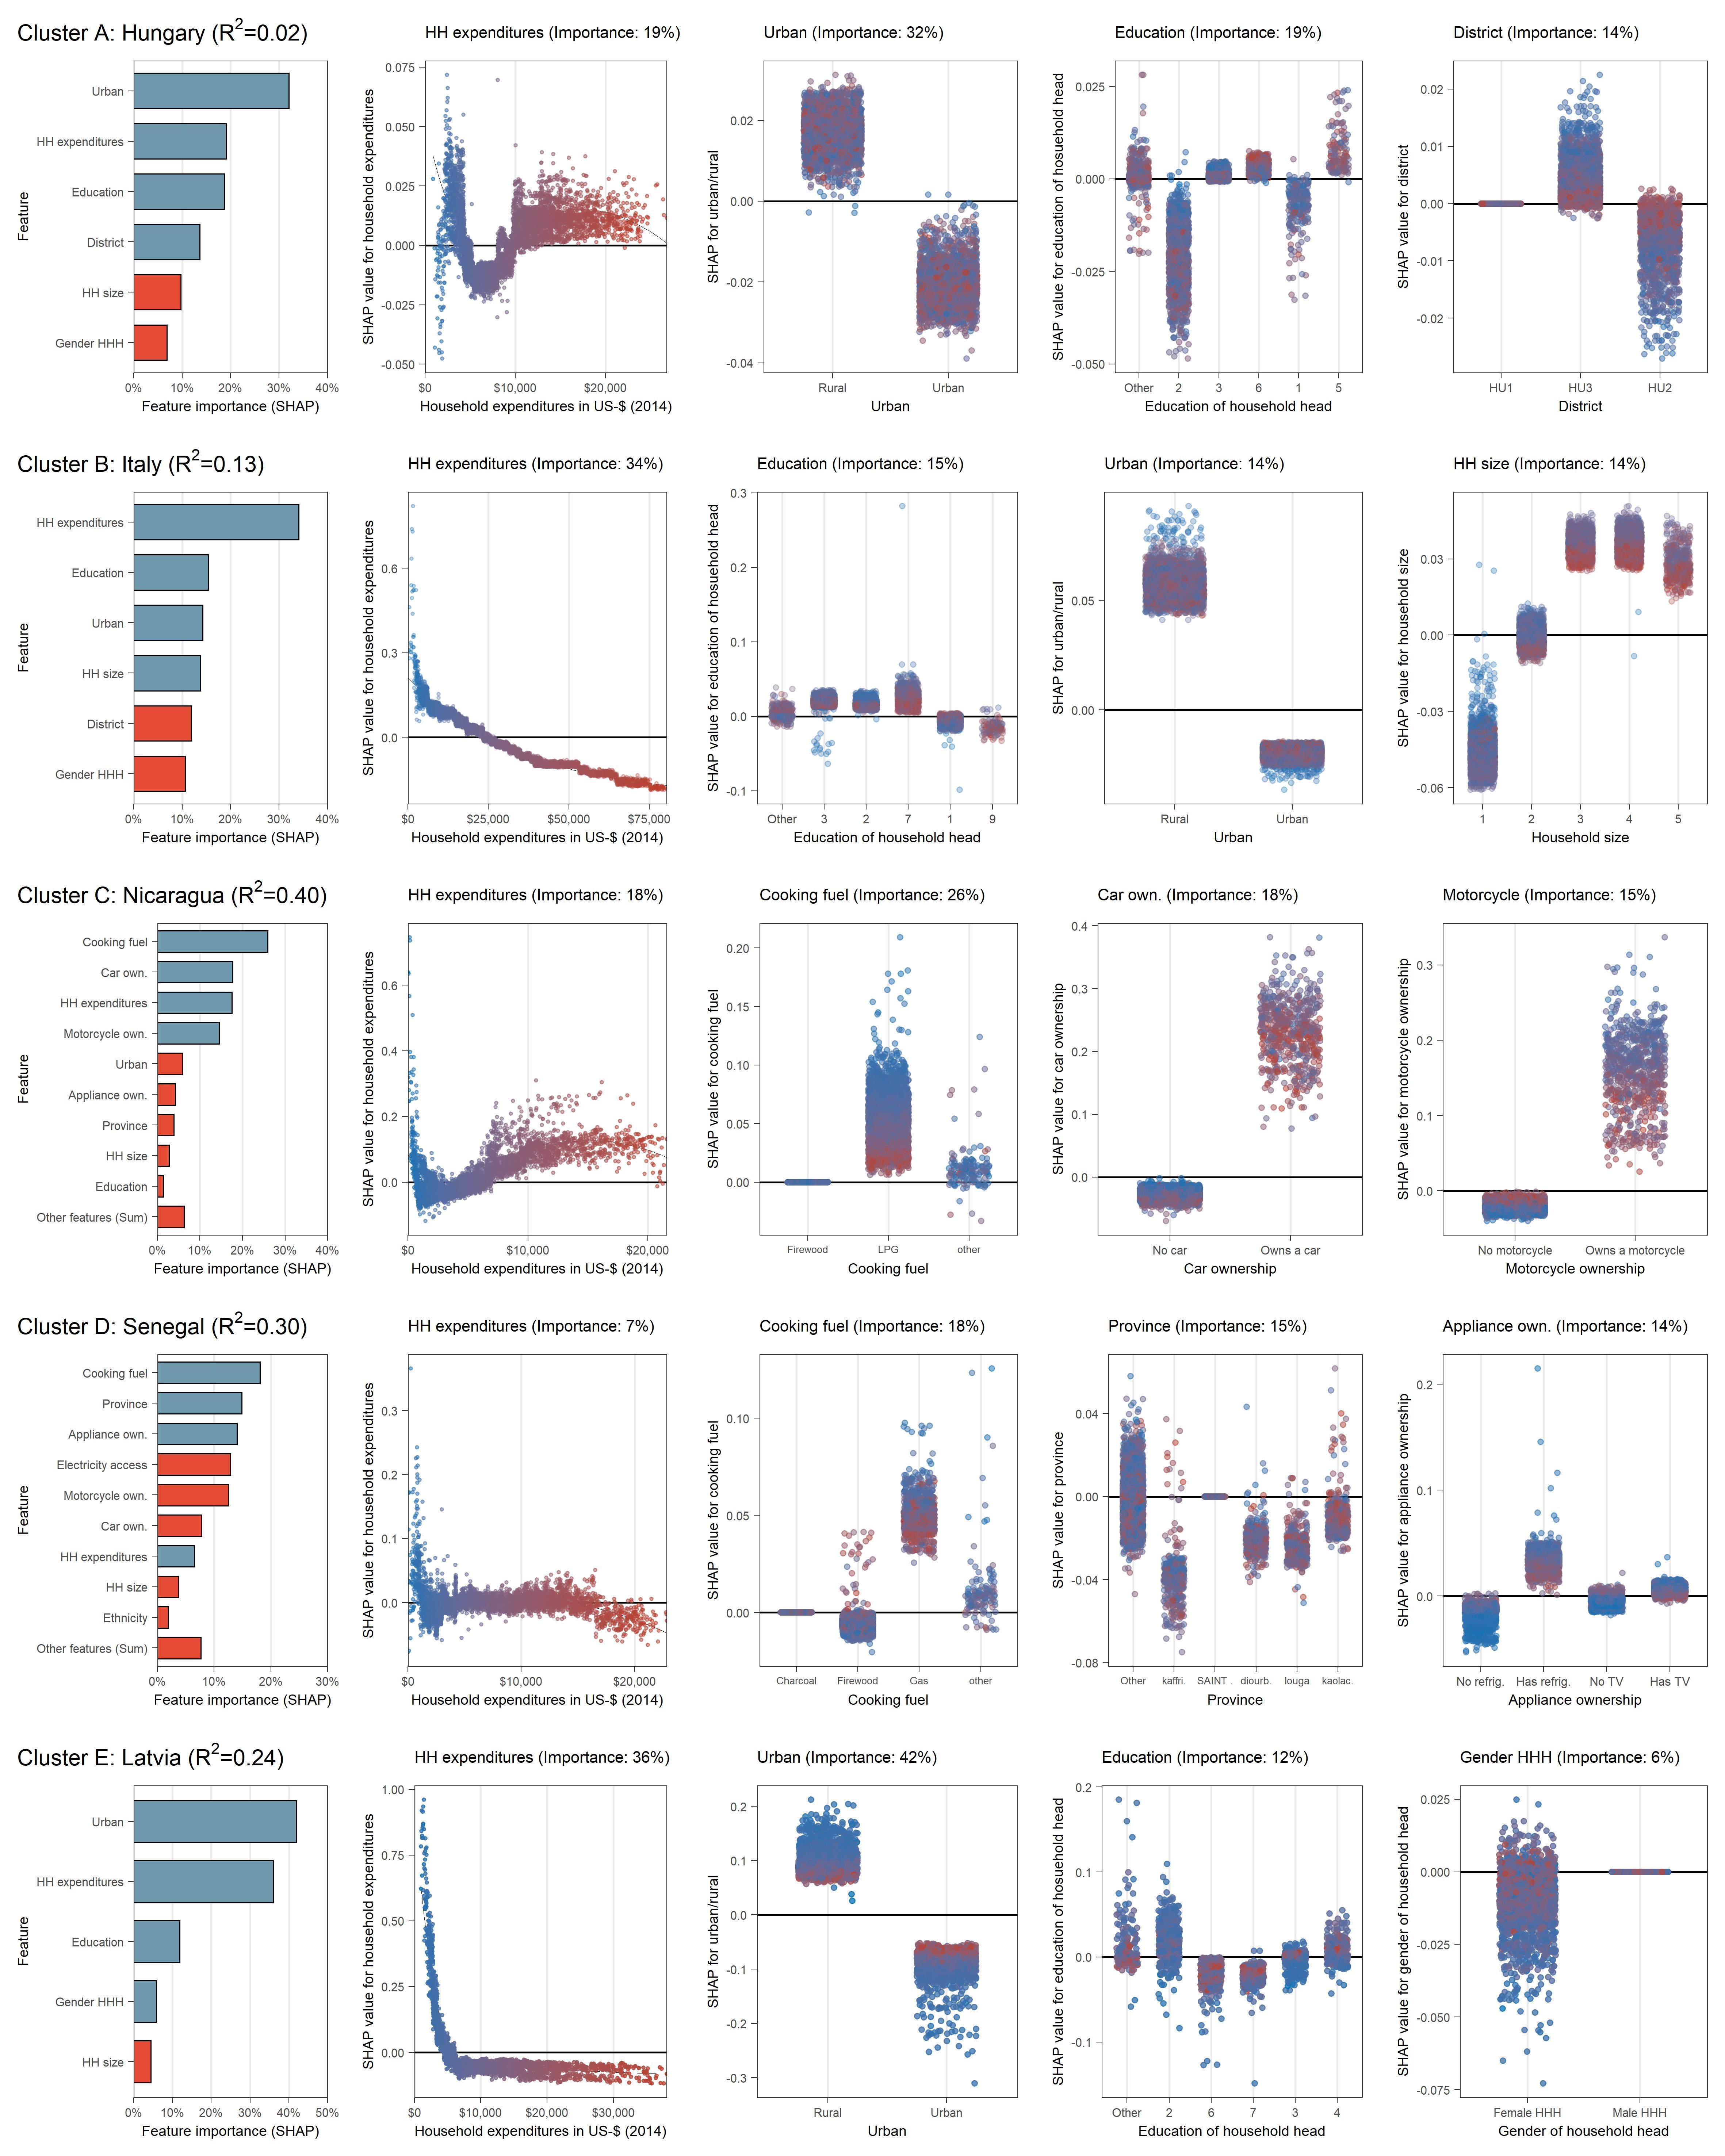
\includegraphics[width=15.5 cm]{Figure 5/Figures_joint_1}
    \caption{Partial dependence plots (SHAP) for one country in clusters A to E}
    \label{fig:fig_5_1}
    \begin{subcaption}
    This figure shows SHAP-values for predicting carbon intensity over feature values for one representative country in each country-cluster in rows. All values are from the testing set. The bar chart displays normalized average absolute SHAP-values for all features. Features with less than 3\% of normalized SHAP-values are subsumed as "Other features (Sum)". Charts show SHAP-values over total household expenditures for all countries and for the three most important features in each country besides total household expenditures. Colors represent household expenditures with blue (red) colors indicating lower (higher) household expenditures. See also Appendix REF to REF.
    \end{subcaption}
\end{figure}

\begin{figure}[ht!]
    \centering
    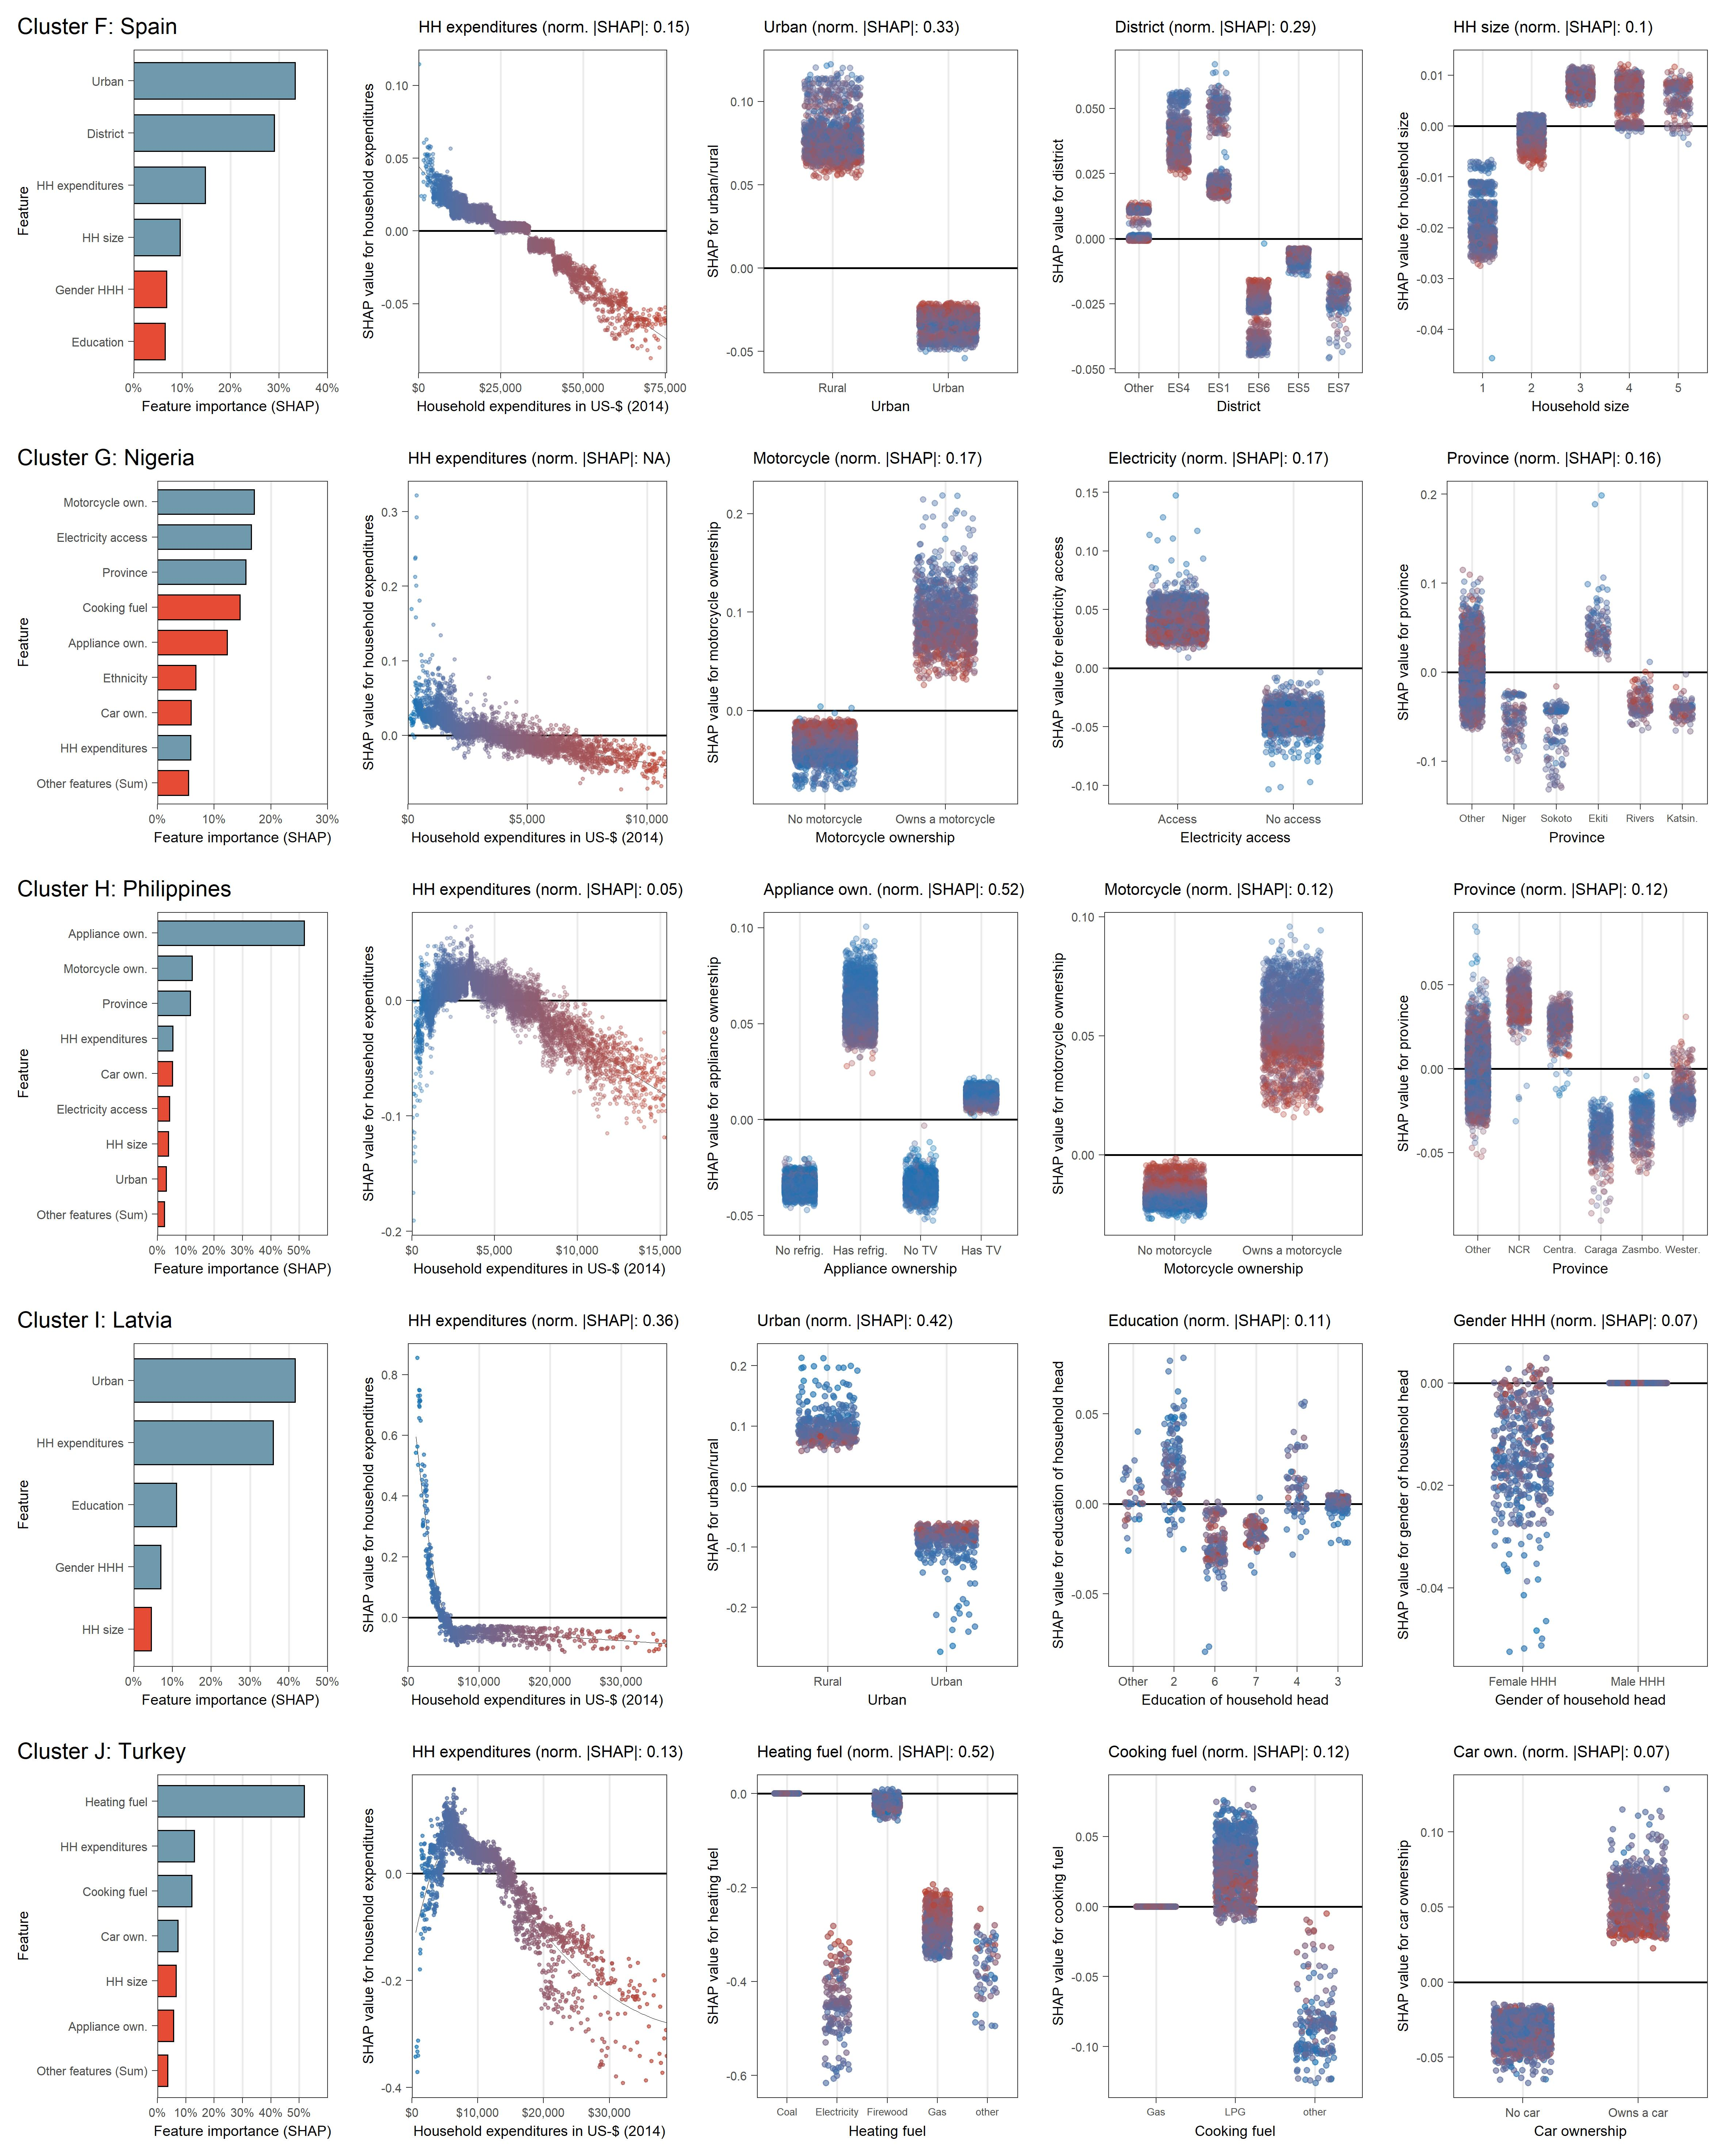
\includegraphics[width=15.5 cm]{Figure 5/Figures_joint_2}
    \caption{Partial dependence plots (SHAP) for one country in clusters F to J}
    \label{fig:fig_5_2}
    \begin{subcaption}
    This figure shows SHAP-values for predicting carbon intensity over feature values for one representative country in each country-cluster in rows. All values are from the testing set. The bar chart displays normalized average absolute SHAP-values for all features. Features with less than 3\% of normalized SHAP-values are subsumed as "Other features (Sum)". Charts show SHAP-values over total household expenditures for all countries and for the three most important features in each country besides total household expenditures. Colors represent household expenditures with blue (red) colors indicating lower (higher) household expenditures. See also Appendix REF to REF
    \end{subcaption}
\end{figure}

\begin{figure}[ht!]
    \centering
    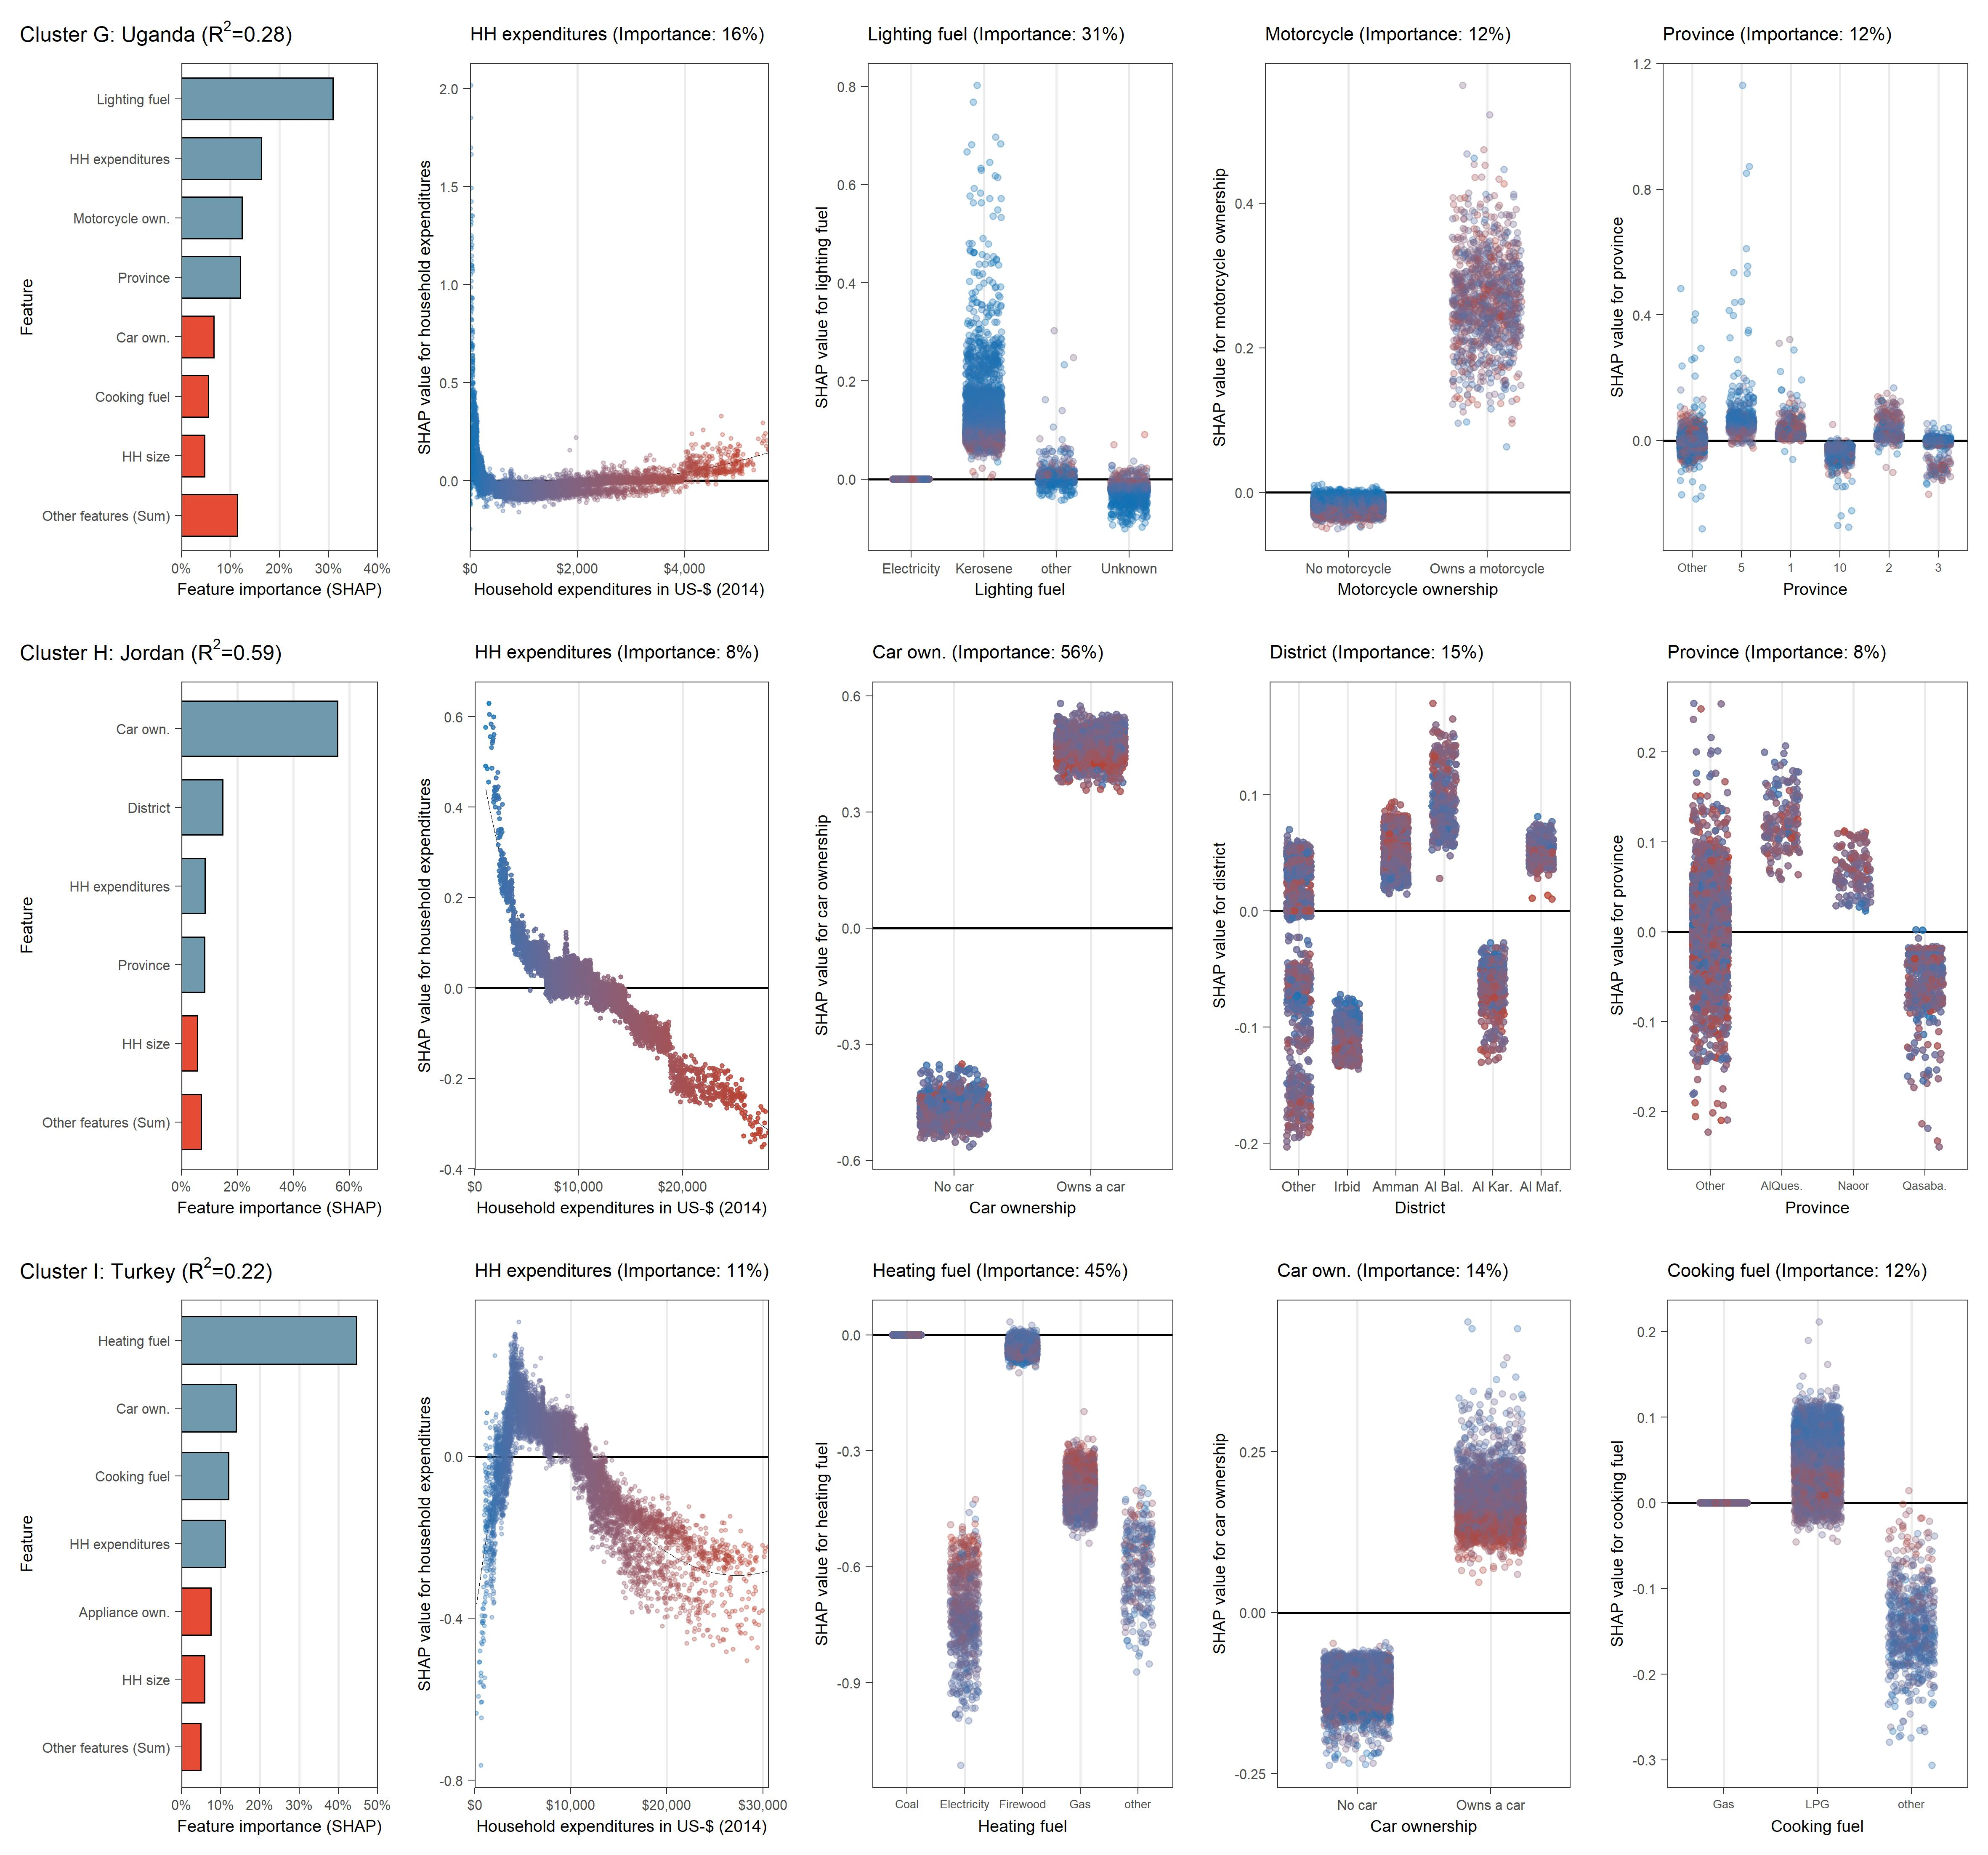
\includegraphics[width=15.5 cm]{Figure 5/Figures_joint_3}
    \caption{Partial dependence plots (SHAP) for one country in clusters K to N}
    \label{fig:fig_5_3}
    \begin{subcaption}
    This figure shows SHAP-values for predicting carbon intensity over feature values for one representative country in each country-cluster in rows. All values are from the testing set. The bar chart displays normalized average absolute SHAP-values for all features. Features with less than 3\% of normalized SHAP-values are subsumed as "Other features (Sum)". Charts show SHAP-values over total household expenditures for all countries and for the three most important features in each country besides total household expenditures. Colors represent household expenditures with blue (red) colors indicating lower (higher) household expenditures. See also Appendix REF to REF.
    \end{subcaption}
\end{figure}

\begin{itemize}
    %\item (Tendenziell ginge auch out-of-sample prediction mit detaillierter Auflösung, wie einzelne features (SHAP) zur gesamten Prediction beitragen).
    \item Marginal effects of logit-models per country for easier visualization. Across countries to Appendix.
    %\item Summary statistics
    %\item Show differences between poor and rich households.
    %\item Show differences within poor and rich households.
    %\item One figure: One country (quintiles and boxplots), all countries (poorest quintile and between-quintile differences), all countries (vertical over horizontal inequality)
    %\item Within-quintile differences exceed between-quintile differences
    %\item Horizontal heterogeneity even more pronounced than vertical heterogeneity in majority of countries
    %\item Households that consume more carbon-intensively than others are poorer than others in richer countries and richer than others in poorer countries. Explain basic intuition.
    %\item If within-quintile differences exceed between-quintile differences using differences in income as a main indicator for evaluating heterogeneity is insufficient.
    %\item Learning about the most carbon-intensively consuming households and their characteristics (beyond income) is important.
    %\item Discuss main arguments for single characteristics (possibly already in methods section).
    \item Show results for different characteristics.
    %\item One figure: One country (Marginal effects from Logit-model), Shapley-values from boosted regression trees
    %\item One figure: Comparing marginal effects from Logit-model across countries
  \item More carbon-intensive households are more likely to own (and use) a car, more likely to use fossil fuels for cooking, such as coal, gas, or LPG, less likely to use firewood, charcoal or biomass for cooking, compared to households cooking with electricity. More likely connected to the electricity grid, more likely to have secondary or higher education, more likely to live in rural areas (in richer countries). Discuss differences in space, across provinces and districts. Depending on the country-context, they are more/less likely to identify with ethnic majorities or minorities.
   %\item Comparing model outcomes across countries. One figure: A: Show classification for single countries with colour codes (order in clusters). B: Show clustering of countries with colour codes.
  \item Discuss differences in instruments: electricity sector instruments, transport sector instruments, international trade policy etc. Highlight main differences: electricity sector characteristics and electrification critical for electricity sector instruments, transport sector policies likely regressive in richer countries, progressive in poorer countries, carbon border adjustments more likely to affect people who consume more carbon-intensive and imported goods and services. Non-consumption impacts probably more severe. (If anything, possibly also Appendix. I suggest the figure comparing vertical and horizontal aspects here - in Appendix).
\end{itemize}

\paragraph{Impacts of climate policy}

\section{Discussion} \label{sec:discussion}

\begin{itemize}
  \item Discuss role of findings for design of transfers. What is being discussed? LST, tax breaks, infrastructure access. Which transfer tool is applicable in which context?
\item Discuss ``value chain of climate policy implementation''. Discuss literature on public acceptance. Highlight research gaps: Which distributional implications matter to households and why? How could compensation increase public support? Public support of which groups matter for people with political power?
 \item Discuss role of findings for design of different policies (standards, subsidies, brief ?)
 \item Discuss dynamic effects and inaccuracies in modeling approach (tax pass-through, short- vs. medium-term, technological path dependencies/barriers on household-level)
 \item Distinguish results from analyses about climate policy on labour, wealth, impacts, adaptation, co-benefits, co-costs.
\end{itemize}

\section{Conclusion} \label{sec:conclusion}

\begin{itemize}
 \item Differences in income one important criterion for comparing outcomes across groups.
 \item Misses important parts of the picture. Necessary to factor in other characteristics.
 \item More nuanced analyses can help to facilitate discussion on acceptable climate policy.
\end{itemize}

\clearpage

\printbibliography

\clearpage

\appendix

\section{Appendix} \label{sec:appendix}

\subsection{Data cleaning} \label{sec:cleaning}

We describe our approach to collecting, cleaning and homogenizing microdata and to feature engineering for machine learning modeling.

\subsubsection{Collecting household data}



\subsubsection{Cleaning and homogenizing household data}

Building on raw microdata from household budget surveys we perform several cleaning steps in order to homogenize datasets across countries.

\begin{itemize}
    \item We address outliers of household expenditures at the item-level. We consider any observation an outlier if it it in the $99^{th}$ quantile of all non-zero expenditures. We replace this observation with item-level median expenditures.
    \item We remove observations if expenditures are negative, for example, if households sell items.
    \item We remove duplicates from our sample. We check separately for duplicates at the level of household-level information, but also at the level of item expenditures: We consider households spending the same amount of money on the same items duplicates.
    \item We remove all households from our sample if aggregate expenditures exceed mean expenditures by five standard deviations ($z>5$).
    \item We use inflation rates from \textcite{IMF.2020} and exchange rates from the \textcite{WorldBankGroup.2023} to convert all local currencies to US-\$ for the year 2014. Expenditures from surveys conducted before 2014 are inflated; expenditures from surveys after 2014 are deflated. This ensures consistency with calculated $CO_{2}$-emissions as they refer to the year 2014. This approach does however neglect that expenditure shares may change with inflation.
    \item We create matching tables to assign country-level expenditure items to 65 aggregate sectors and to four broad expenditure categories (energy, food, goods, services). Items, that are difficult to match to a specific sector or to a specific category, e.g., 'other expenses', are matched to artificial sectors and categories labeled 'other'. We delete observations for items indicating aggregate categories, if this would lead to double-counting of single expenditures. We delete observations for items indicating taxes, since including them would prove inaccurate to calculate expenditure shares and because items indicating tax payments are not available in each country. We also identify items indicating energy use and create separate columns listing expenditures for different energy items, such as electricity, gasoline, diesel, kerosene, LPG, natural gas, charcoal, hard coal, firewood and other biomass. All matching tables are available through a separate stable online repository (INSERT LINK).
\end{itemize}

% tracking and documenting removals

\subsubsection{Feature engineering} \label{sec:featureengineering}

Building on our homogenized dataset, we perform feature engineering on our variables (features) before performing analyses with BRT.

\begin{itemize}
    \item We exclude any feature with missing variation (for four countries).
    \item We exclude categorical feature with high granularity (such as district-level identifiers).
    \item We exclude any feature with missing values-
    \item We remove the minimum number of features necessary to avoid high levels of correlation ($r>0.9$) between features.
    \item We code observations as "other" for each feature (except province-level, district-level and urban-/rural-identifiers) which account for less than 5\% of all observations.
    \item All country-level feature sets include total household expenditures (in US-\$ 2014) and household size. The minimum number of included features is X (for Y) and the maximum number of included feature is X (for Z).
\end{itemize}

\subsection{Policy simulation}\label{sec:policysimulation}

We show that heterogeneity in household-level carbon intensity of consumption is equivalent to heterogeneity in household-level carbon pricing incidence, assuming that producers pass-on carbon prices to consumers and that the carbon pricing incidence reflects over-night costs to households without demand responses.

\begin{equation}
    CPI_{i} = \frac{E_{i}*\tau}{C_{i}}
\end{equation}

Tau proportionaler Faktor. Ausdruck in \% as $\frac{USD_{\tau}}{USD_{i}}$ or in $\frac{kgCO_{2}}{USD_{i}}$ with $\tau$ in $\frac{USD}{kgCO_{2}}$.

\clearpage

\renewcommand\thefigure{\thesection.\arabic{figure}}
\renewcommand\thetable{\thesection.\arabic{table}}
\setcounter{figure}{0}
\setcounter{table}{0}

\subsection{Supplementary figures} \label{sec:figures}

\begin{figure}[ht!]
  \centering
  \caption{Engel curves: expenditure shares over total household expenditures - Part A} \label{fig:A1}
  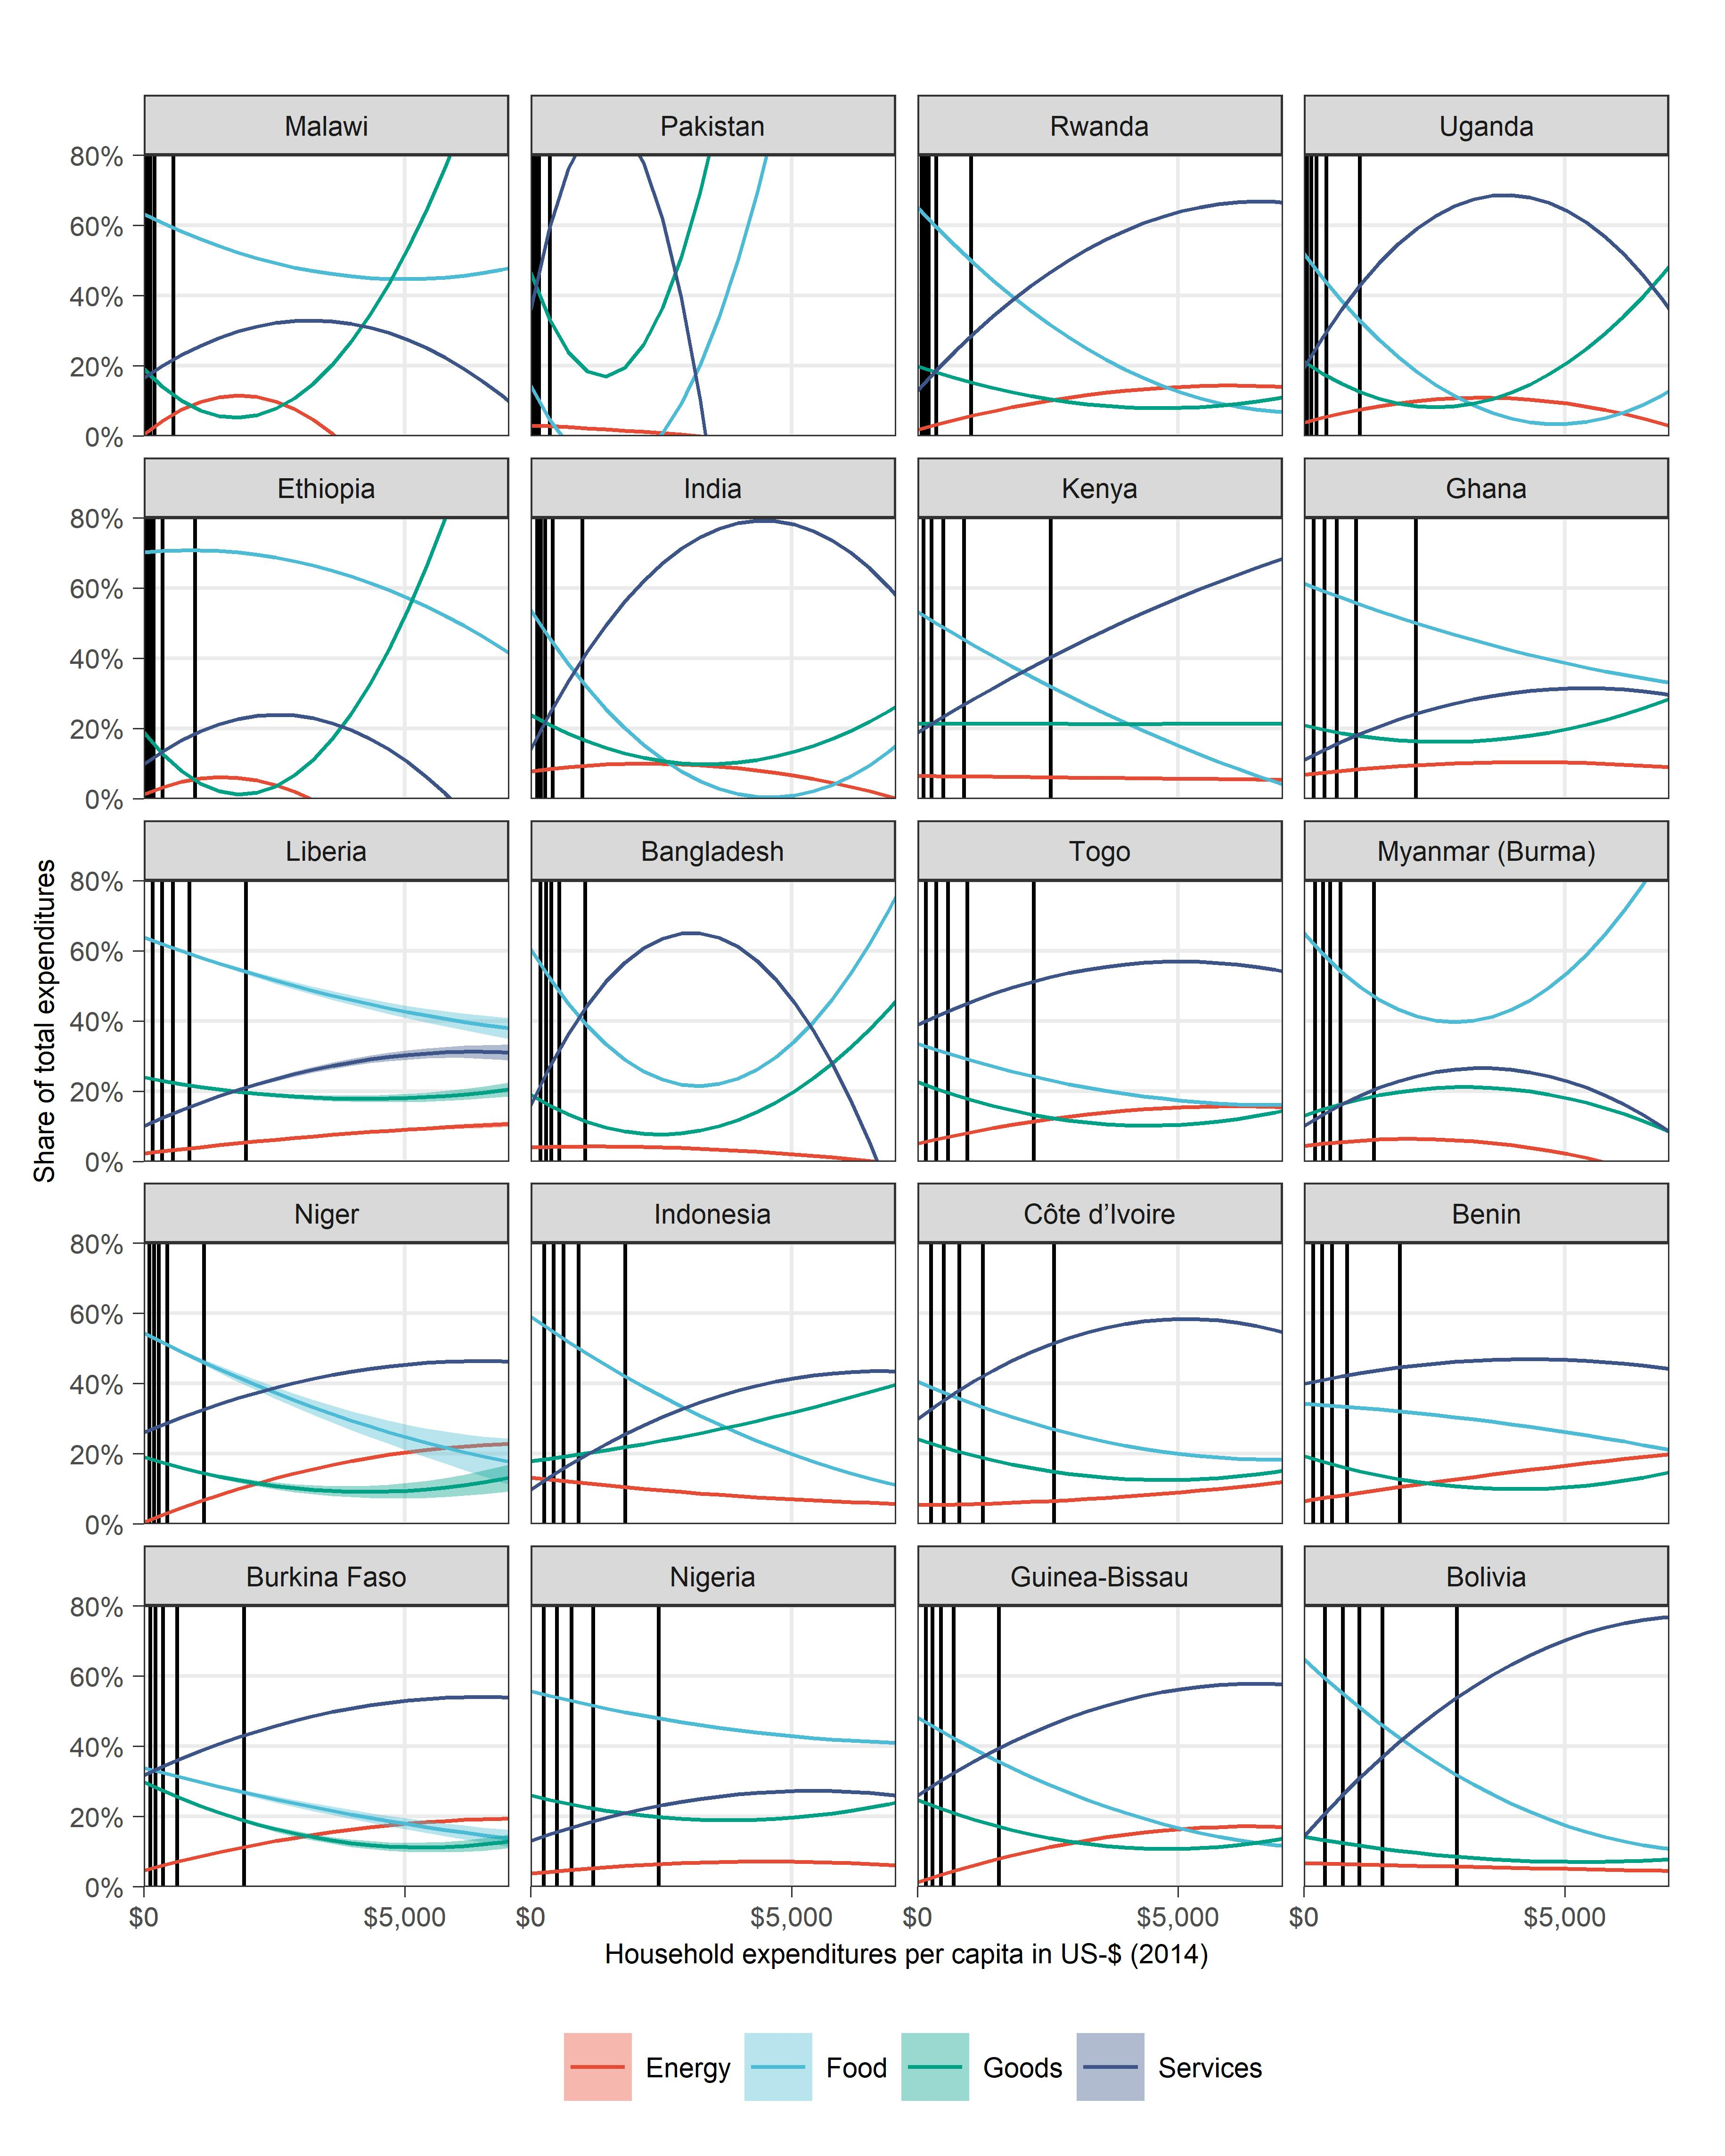
\includegraphics{Analysis_Parametric_Engel_Curves/Parametric_EC_0_A}
  \begin{subcaption}
    This figure displays fitted lines for parametric and quadratic Engel curves for each consumption category in 20 countries of our sample. Black vertical lines indicate average household expenditures per capita for each expenditure quintile and country.
  \end{subcaption}

\end{figure}

\clearpage

\begin{figure}[ht!]
  \centering
  \caption{Engel curves: expenditure shares over total household expenditures - Part B} \label{fig:A2}
  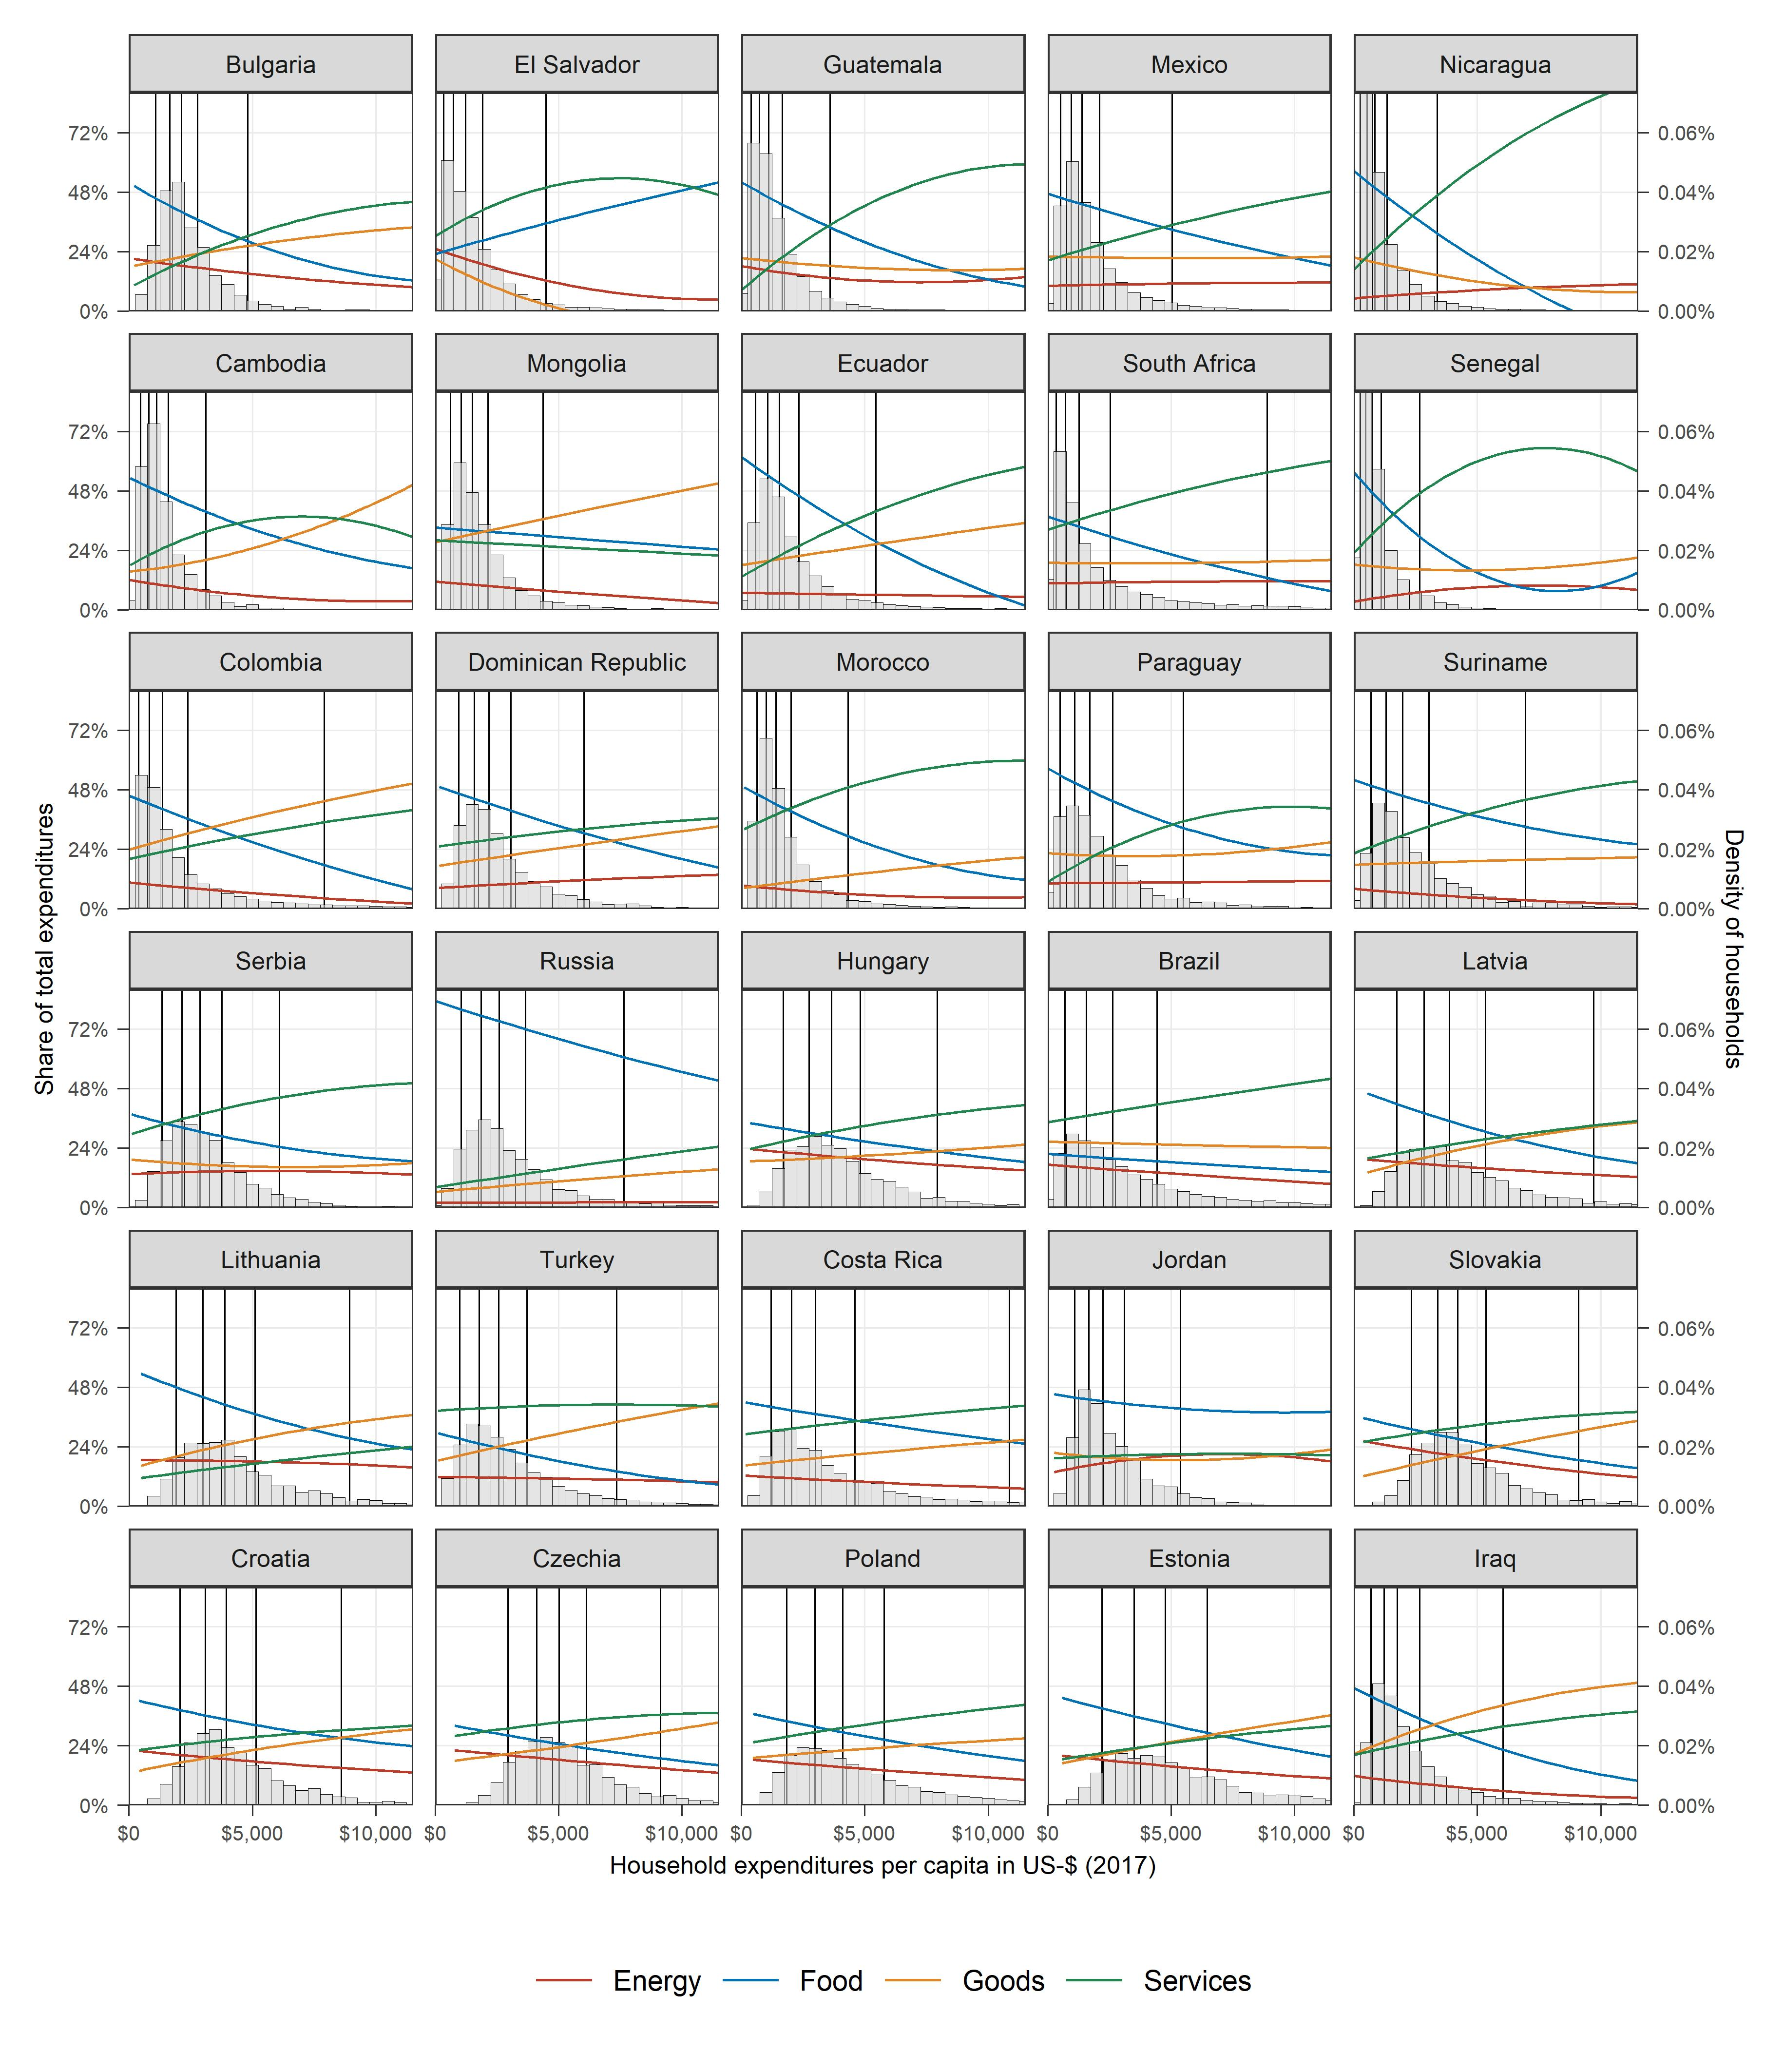
\includegraphics{Analysis_Parametric_Engel_Curves/Parametric_EC_0_B}
  \begin{subcaption}
    This figure displays fitted lines for parametric and quadratic Engel curves for each consumption category in 20 countries of our sample. Black vertical lines indicate average household expenditures per capita for each expenditure quintile and country.
  \end{subcaption}

\end{figure}

\clearpage

% \begin{figure}[ht!]
%   \centering
%   \caption{Engel curves: expenditure shares over total household expenditures - Part C} \label{fig:A3}
%   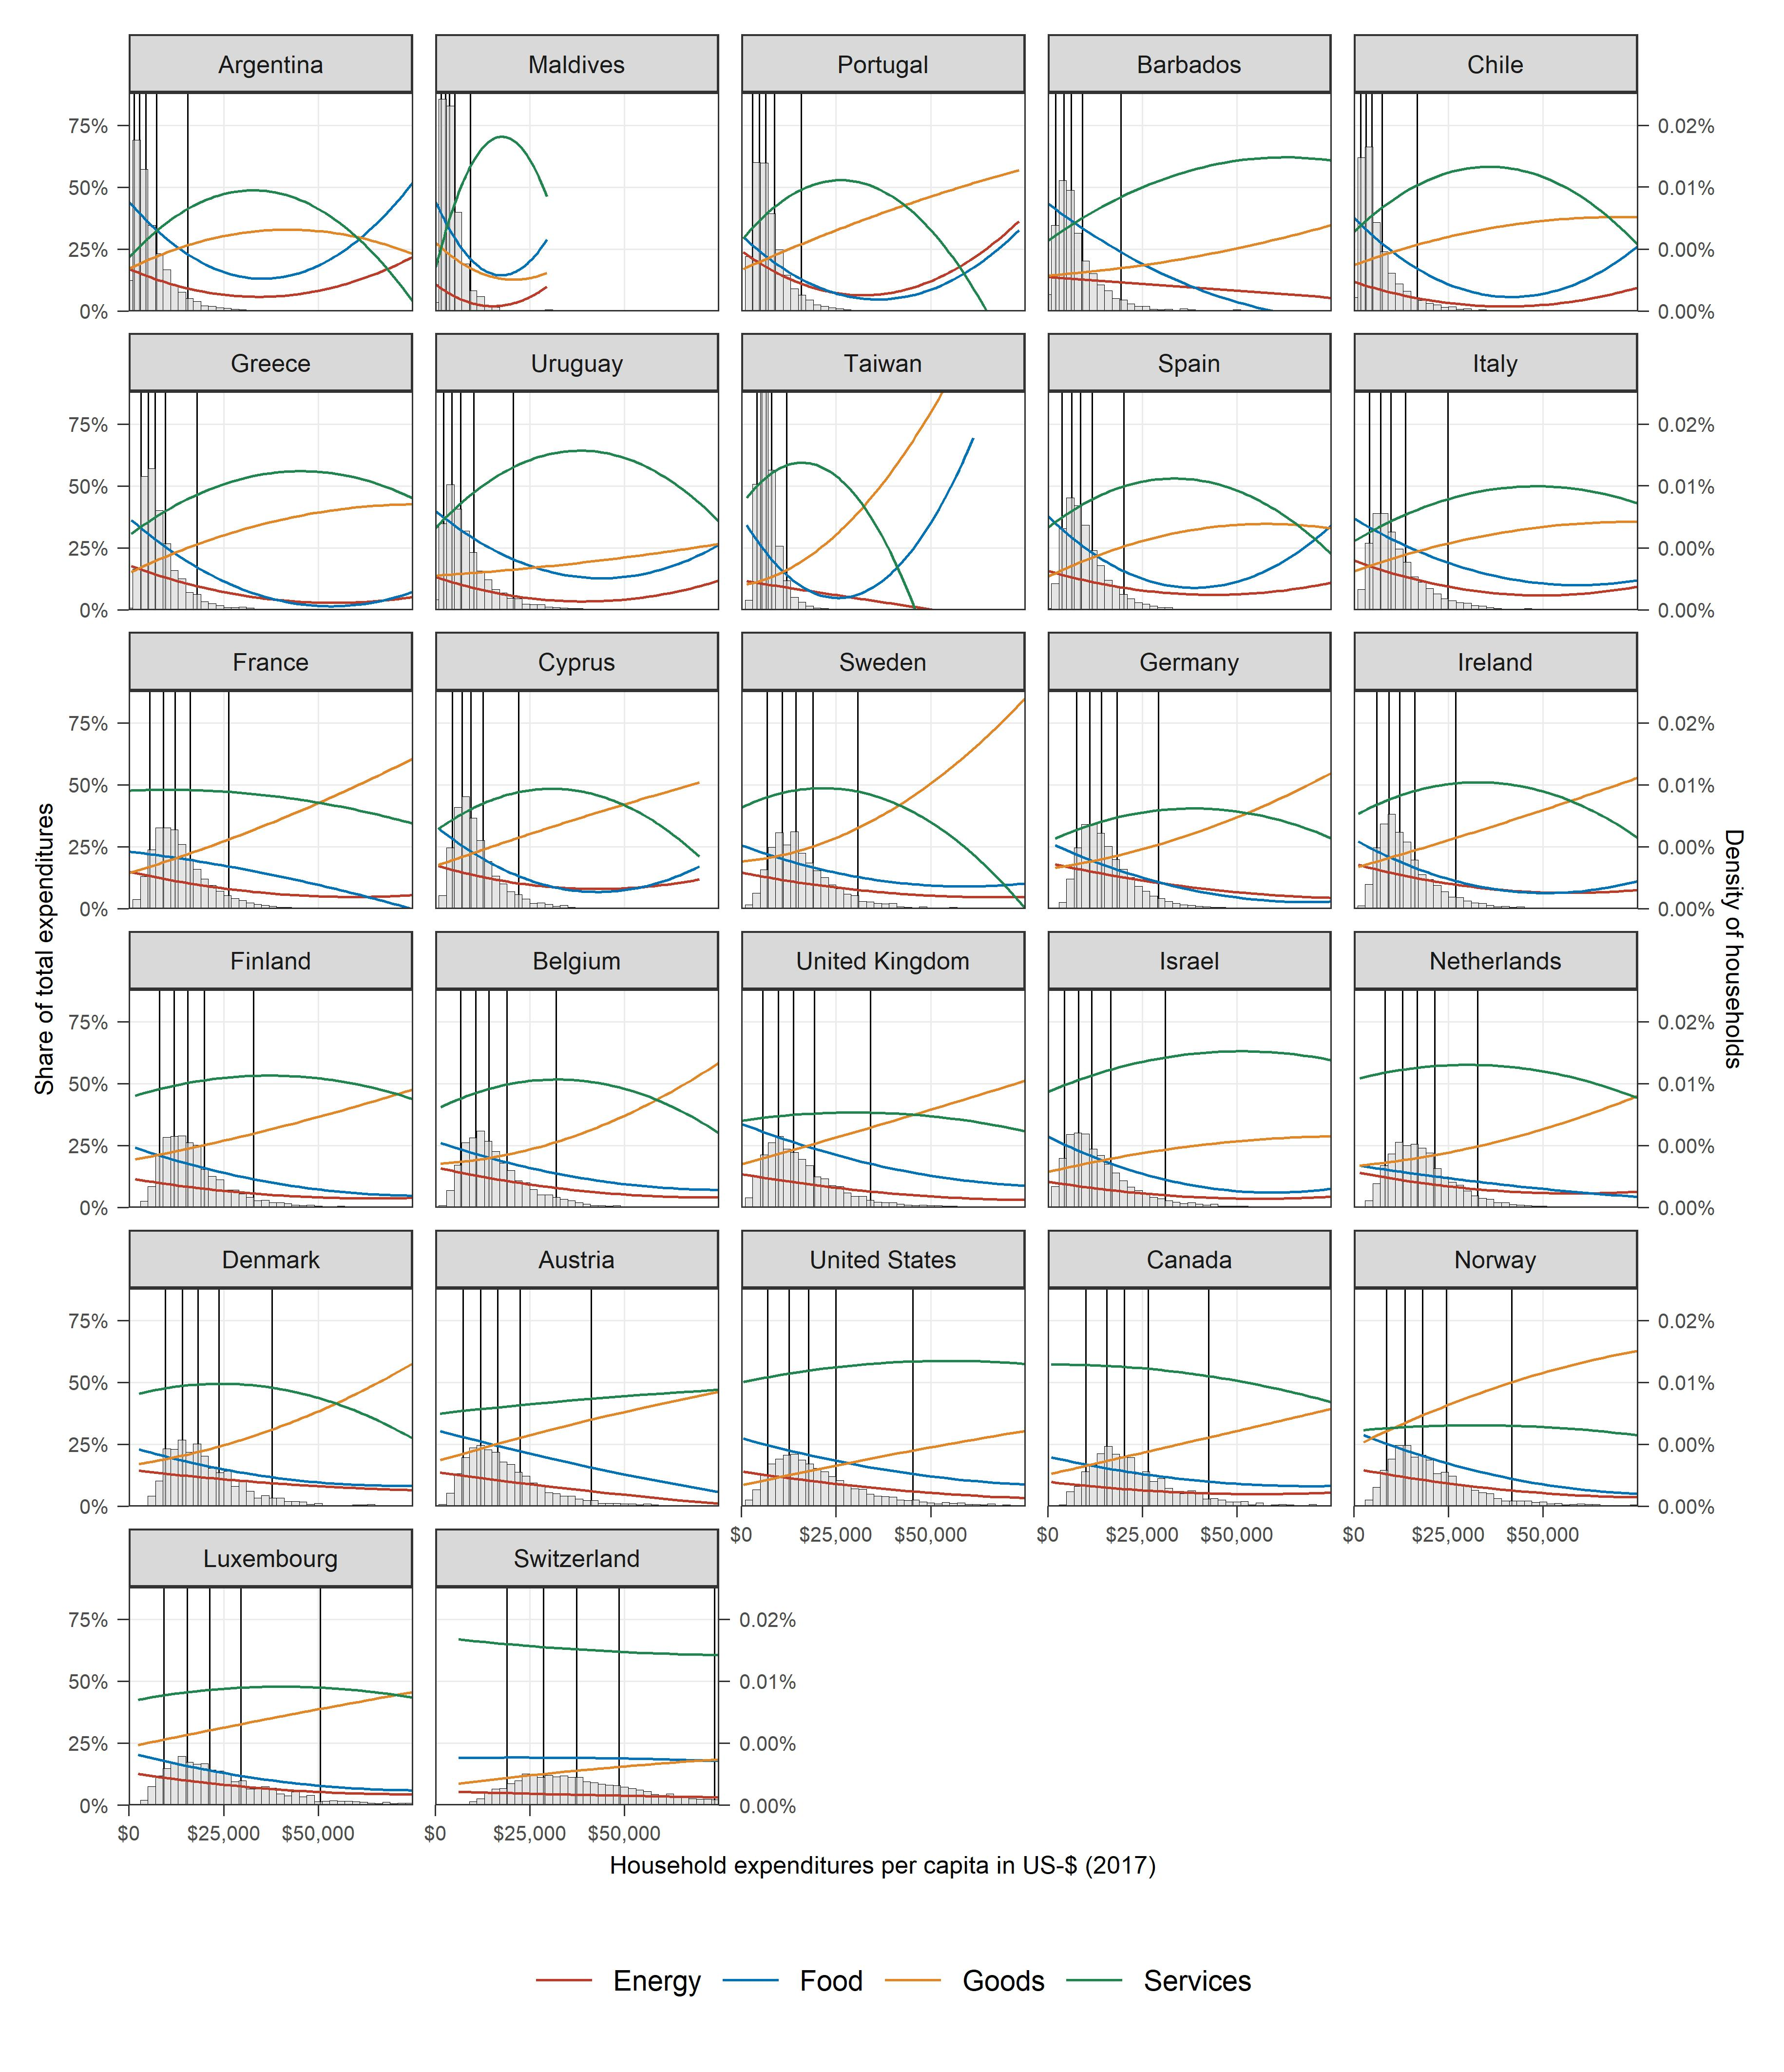
\includegraphics{Analysis_Parametric_Engel_Curves/Parametric_EC_0_C}
%   \begin{subcaption}
%     This figure displays fitted lines for parametric and quadratic Engel curves for each consumption category in 20 countries of our sample. Black vertical lines indicate average household expenditures per capita for each expenditure quintile and country.
%   \end{subcaption}

% \end{figure}

% \clearpage

% \begin{figure}[ht!]
%   \centering
%   \caption{Engel curves: expenditure shares over total household expenditures - Part D} \label{fig:A4}
%   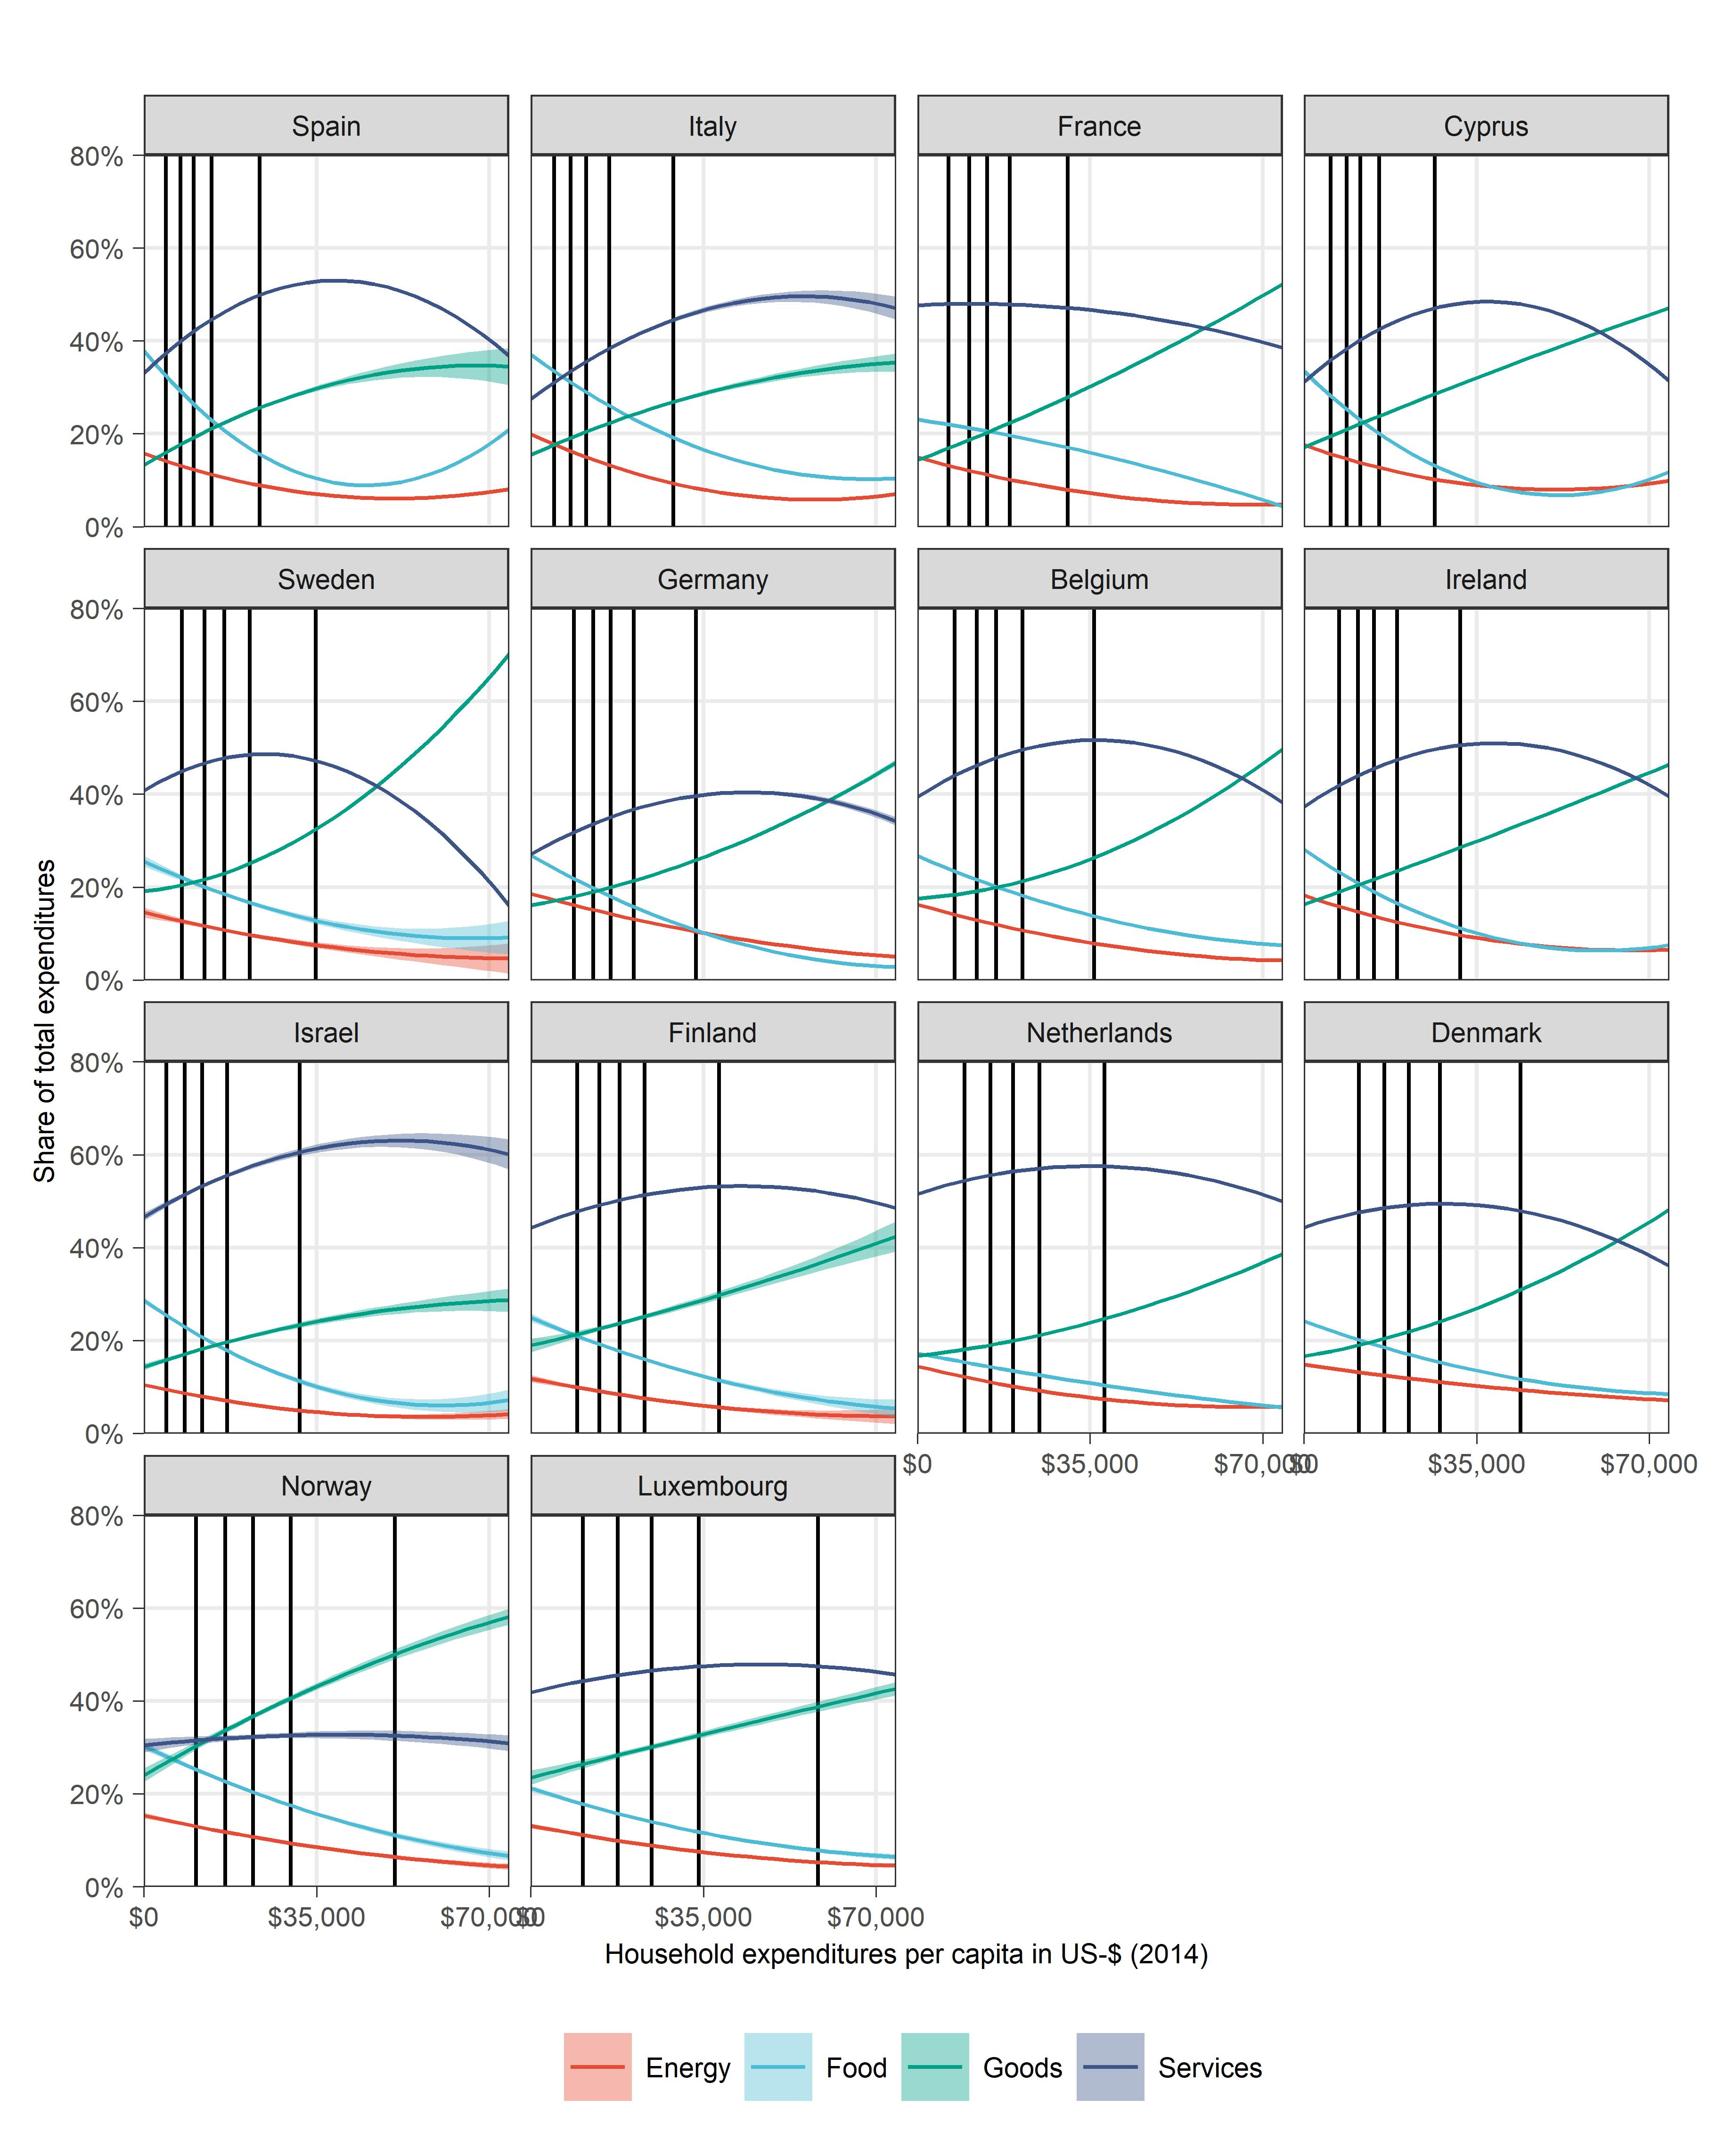
\includegraphics{Analysis_Parametric_Engel_Curves/Parametric_EC_0_D}
%   \begin{subcaption}
%     This figure displays fitted lines for parametric and quadratic Engel curves for each consumption category in 20 countries of our sample. Black vertical lines indicate average household expenditures per capita for each expenditure quintile and country.
%   \end{subcaption}

% \end{figure}

% \clearpage

% Carbon intensities

\begin{figure}[ht!]
  \centering
  \caption{Sectoral carbon intensities from GTAP - Part A} \label{fig:B1}
  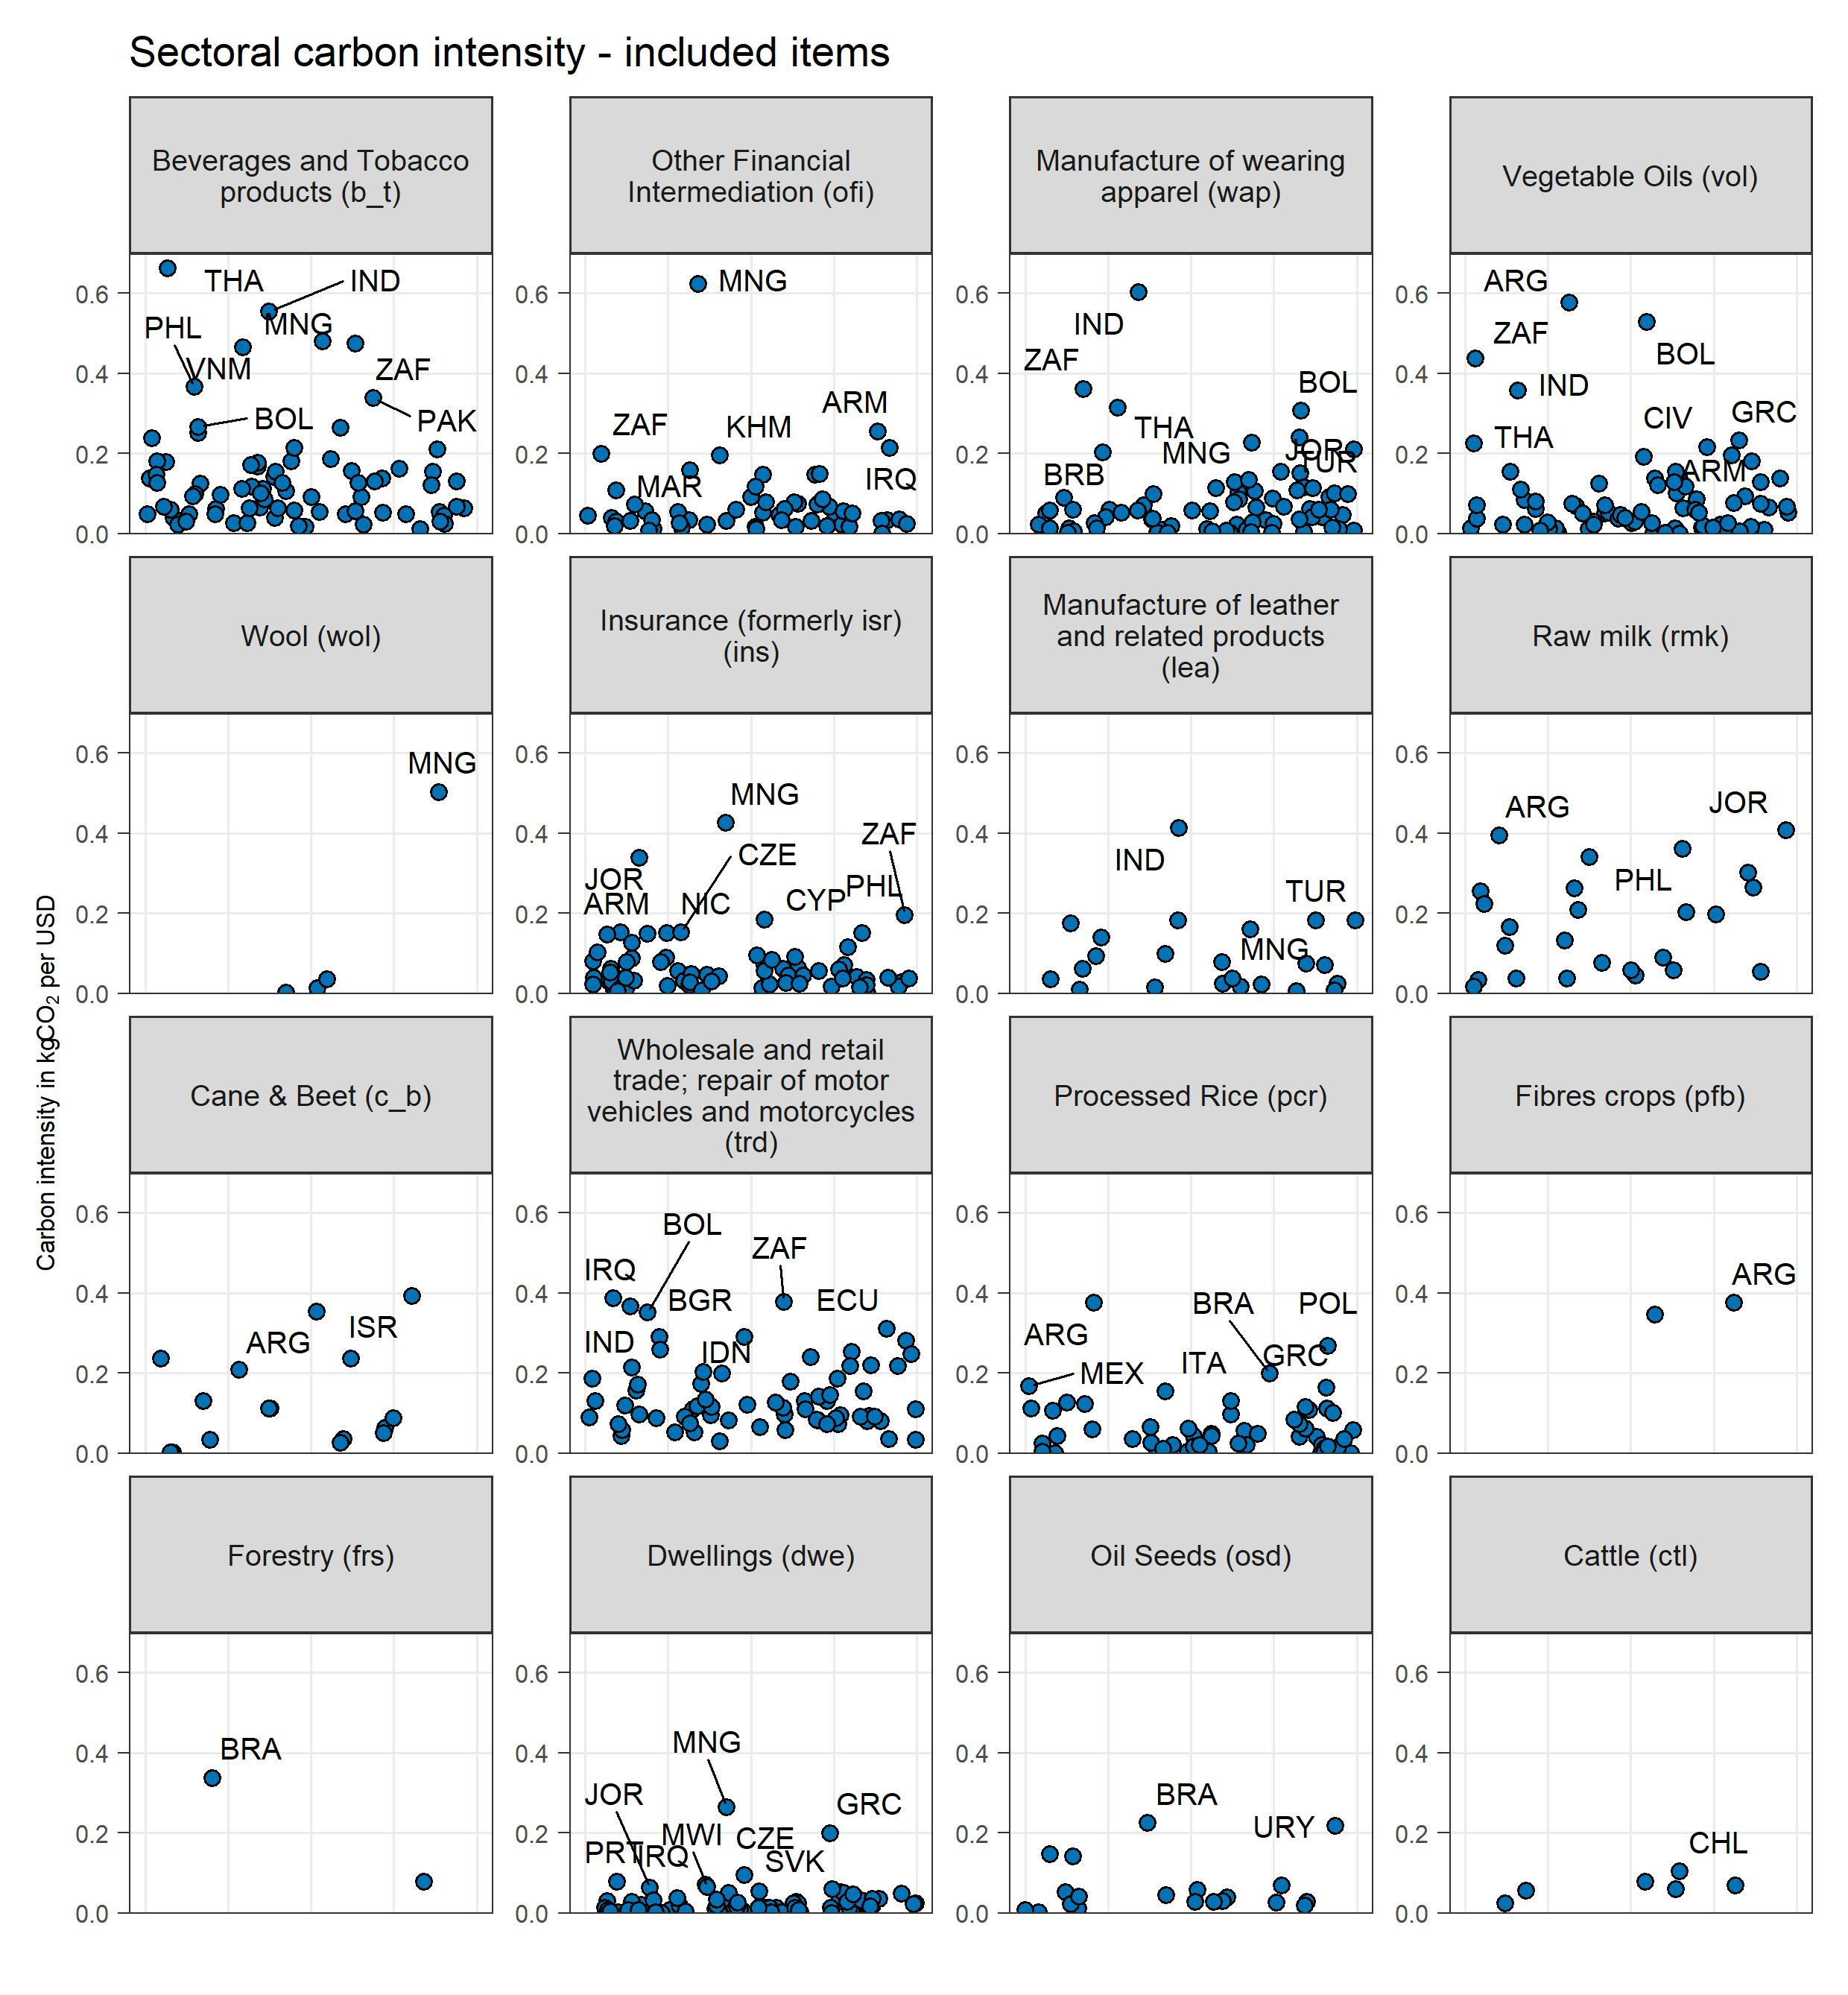
\includegraphics{Analysis_Carbon_Intensities_GTAP/Figure_2.1.1_A}
  \begin{subcaption}
    This figure displays...
  \end{subcaption}

\end{figure}

\clearpage

\begin{figure}[ht!]
  \centering
  \caption{Sectoral carbon intensities from GTAP - Part B} \label{fig:B2}
  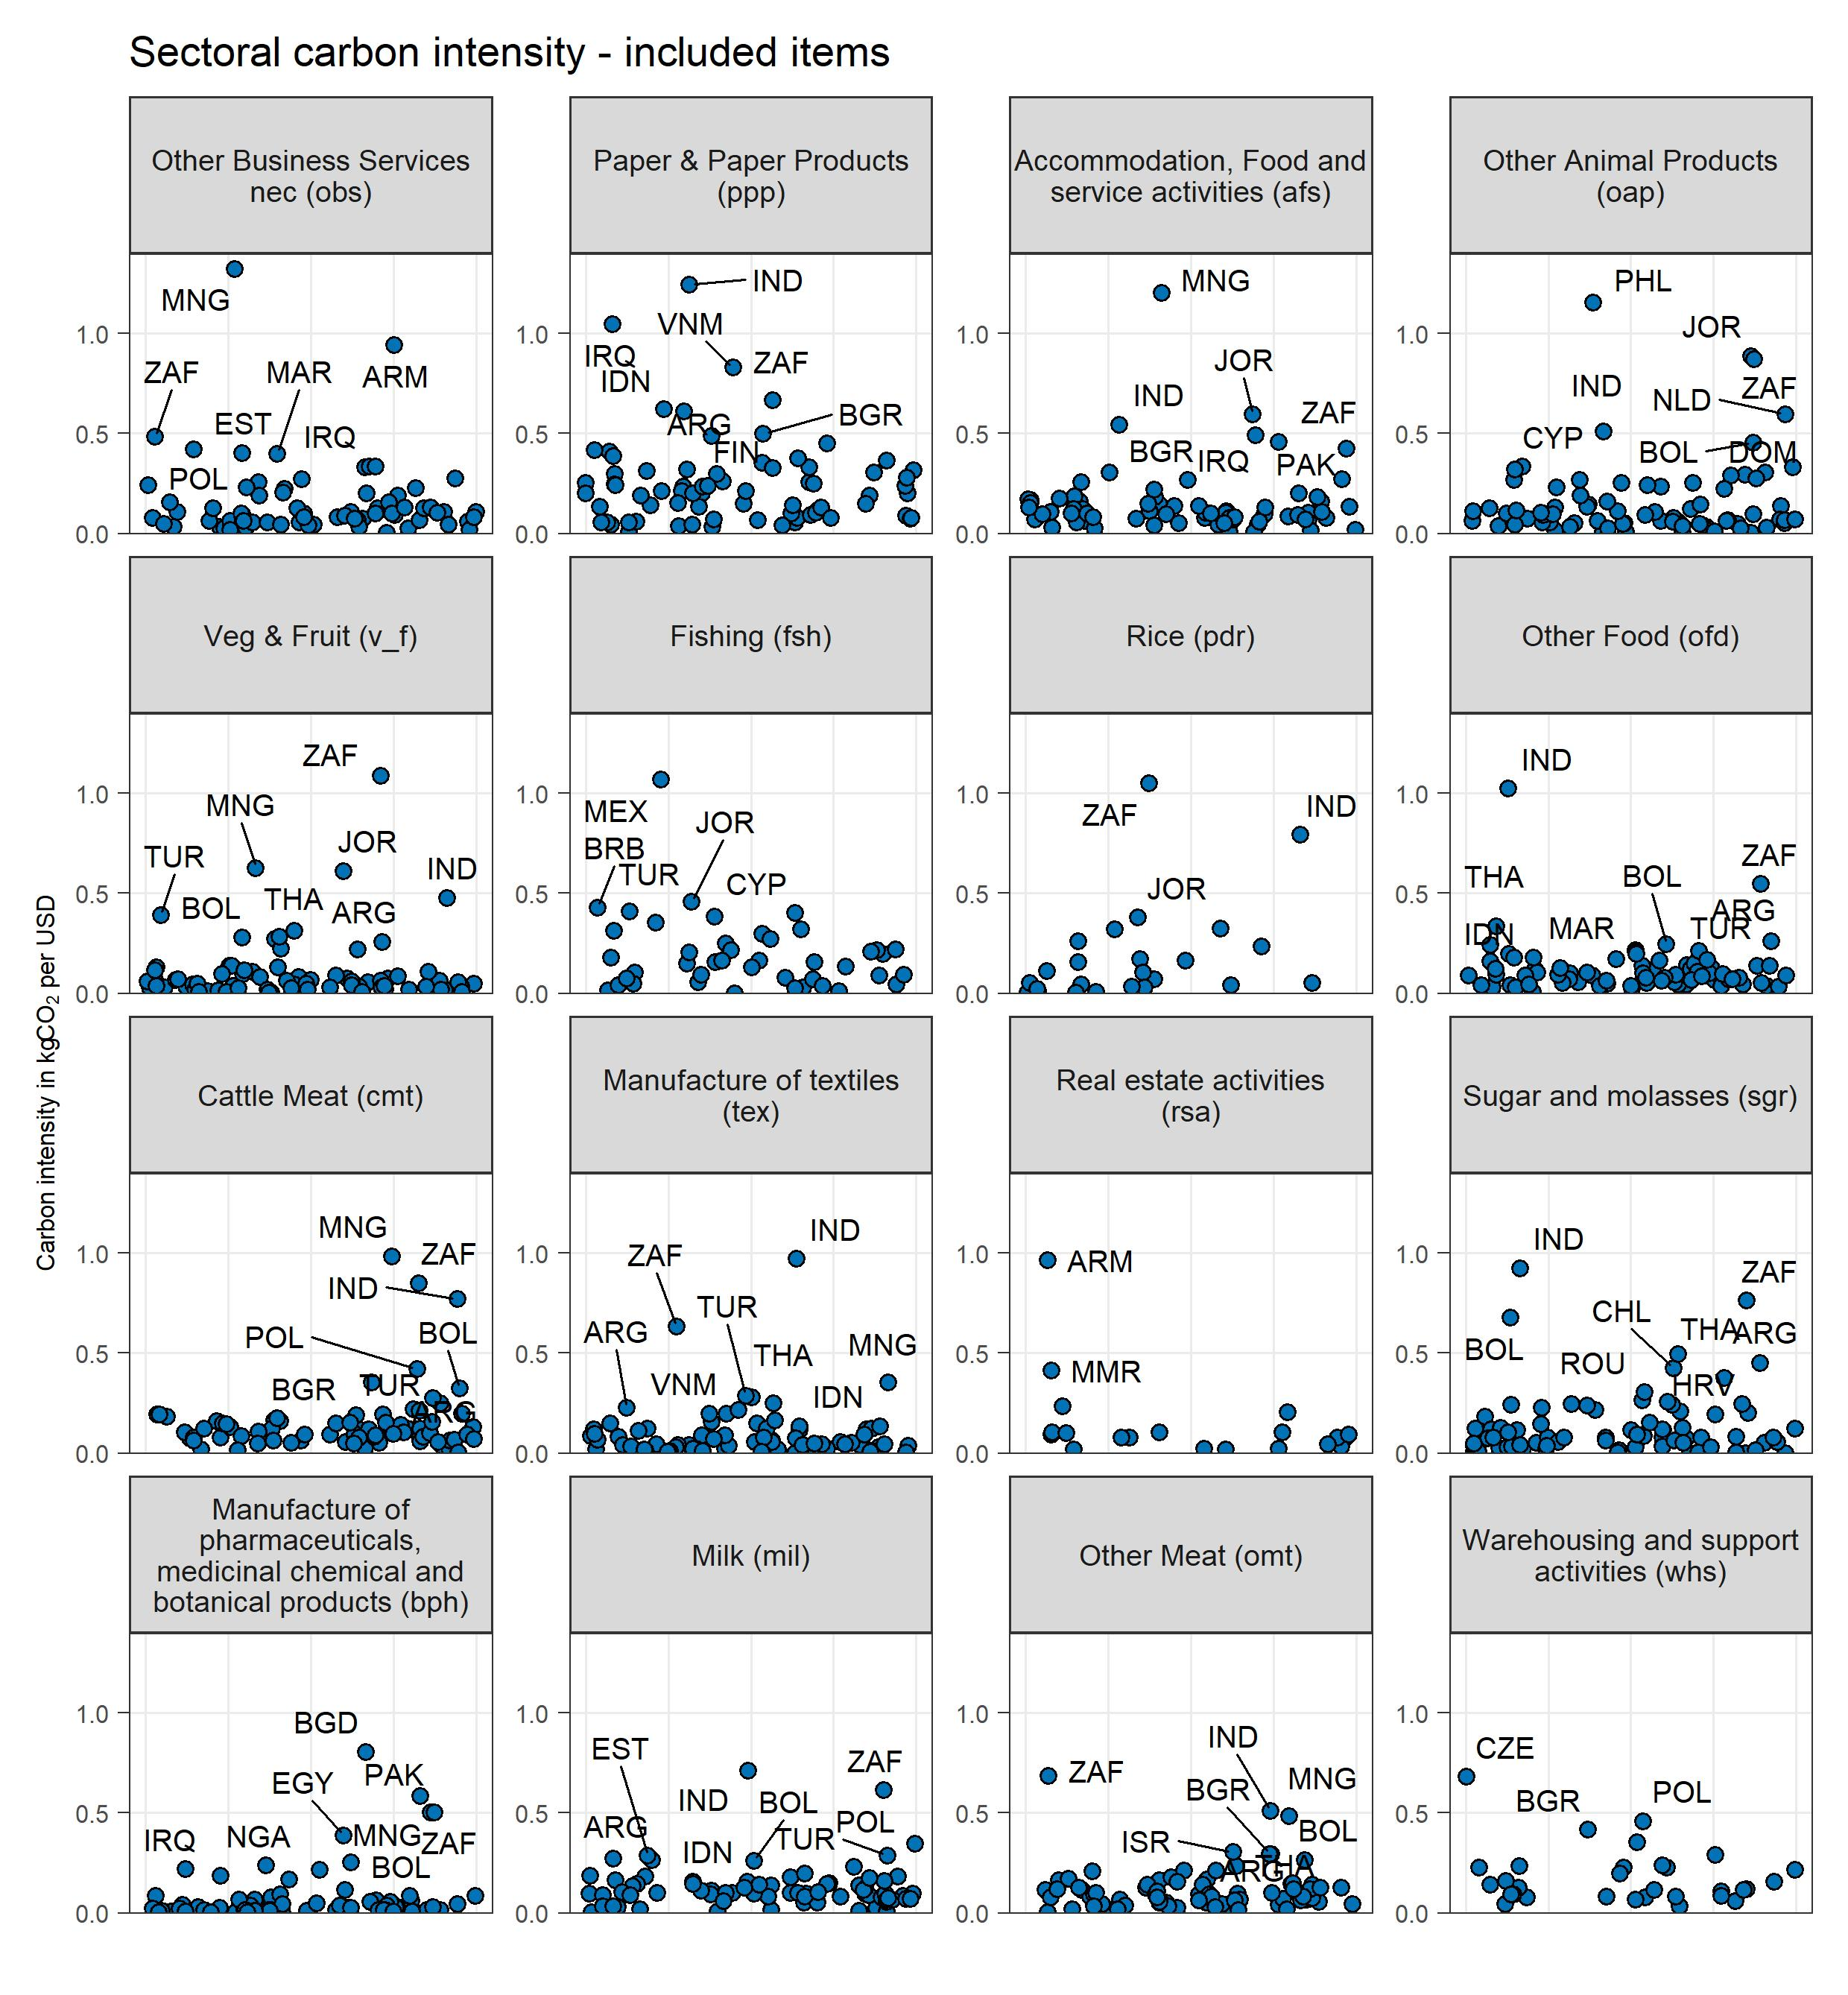
\includegraphics{Analysis_Carbon_Intensities_GTAP/Figure_2.1.1_B}
  \begin{subcaption}
    This figure displays...
  \end{subcaption}

\end{figure}

\clearpage

\begin{figure}[ht!]
  \centering
  \caption{Sectoral carbon intensities from GTAP - Part C} \label{fig:B3}
  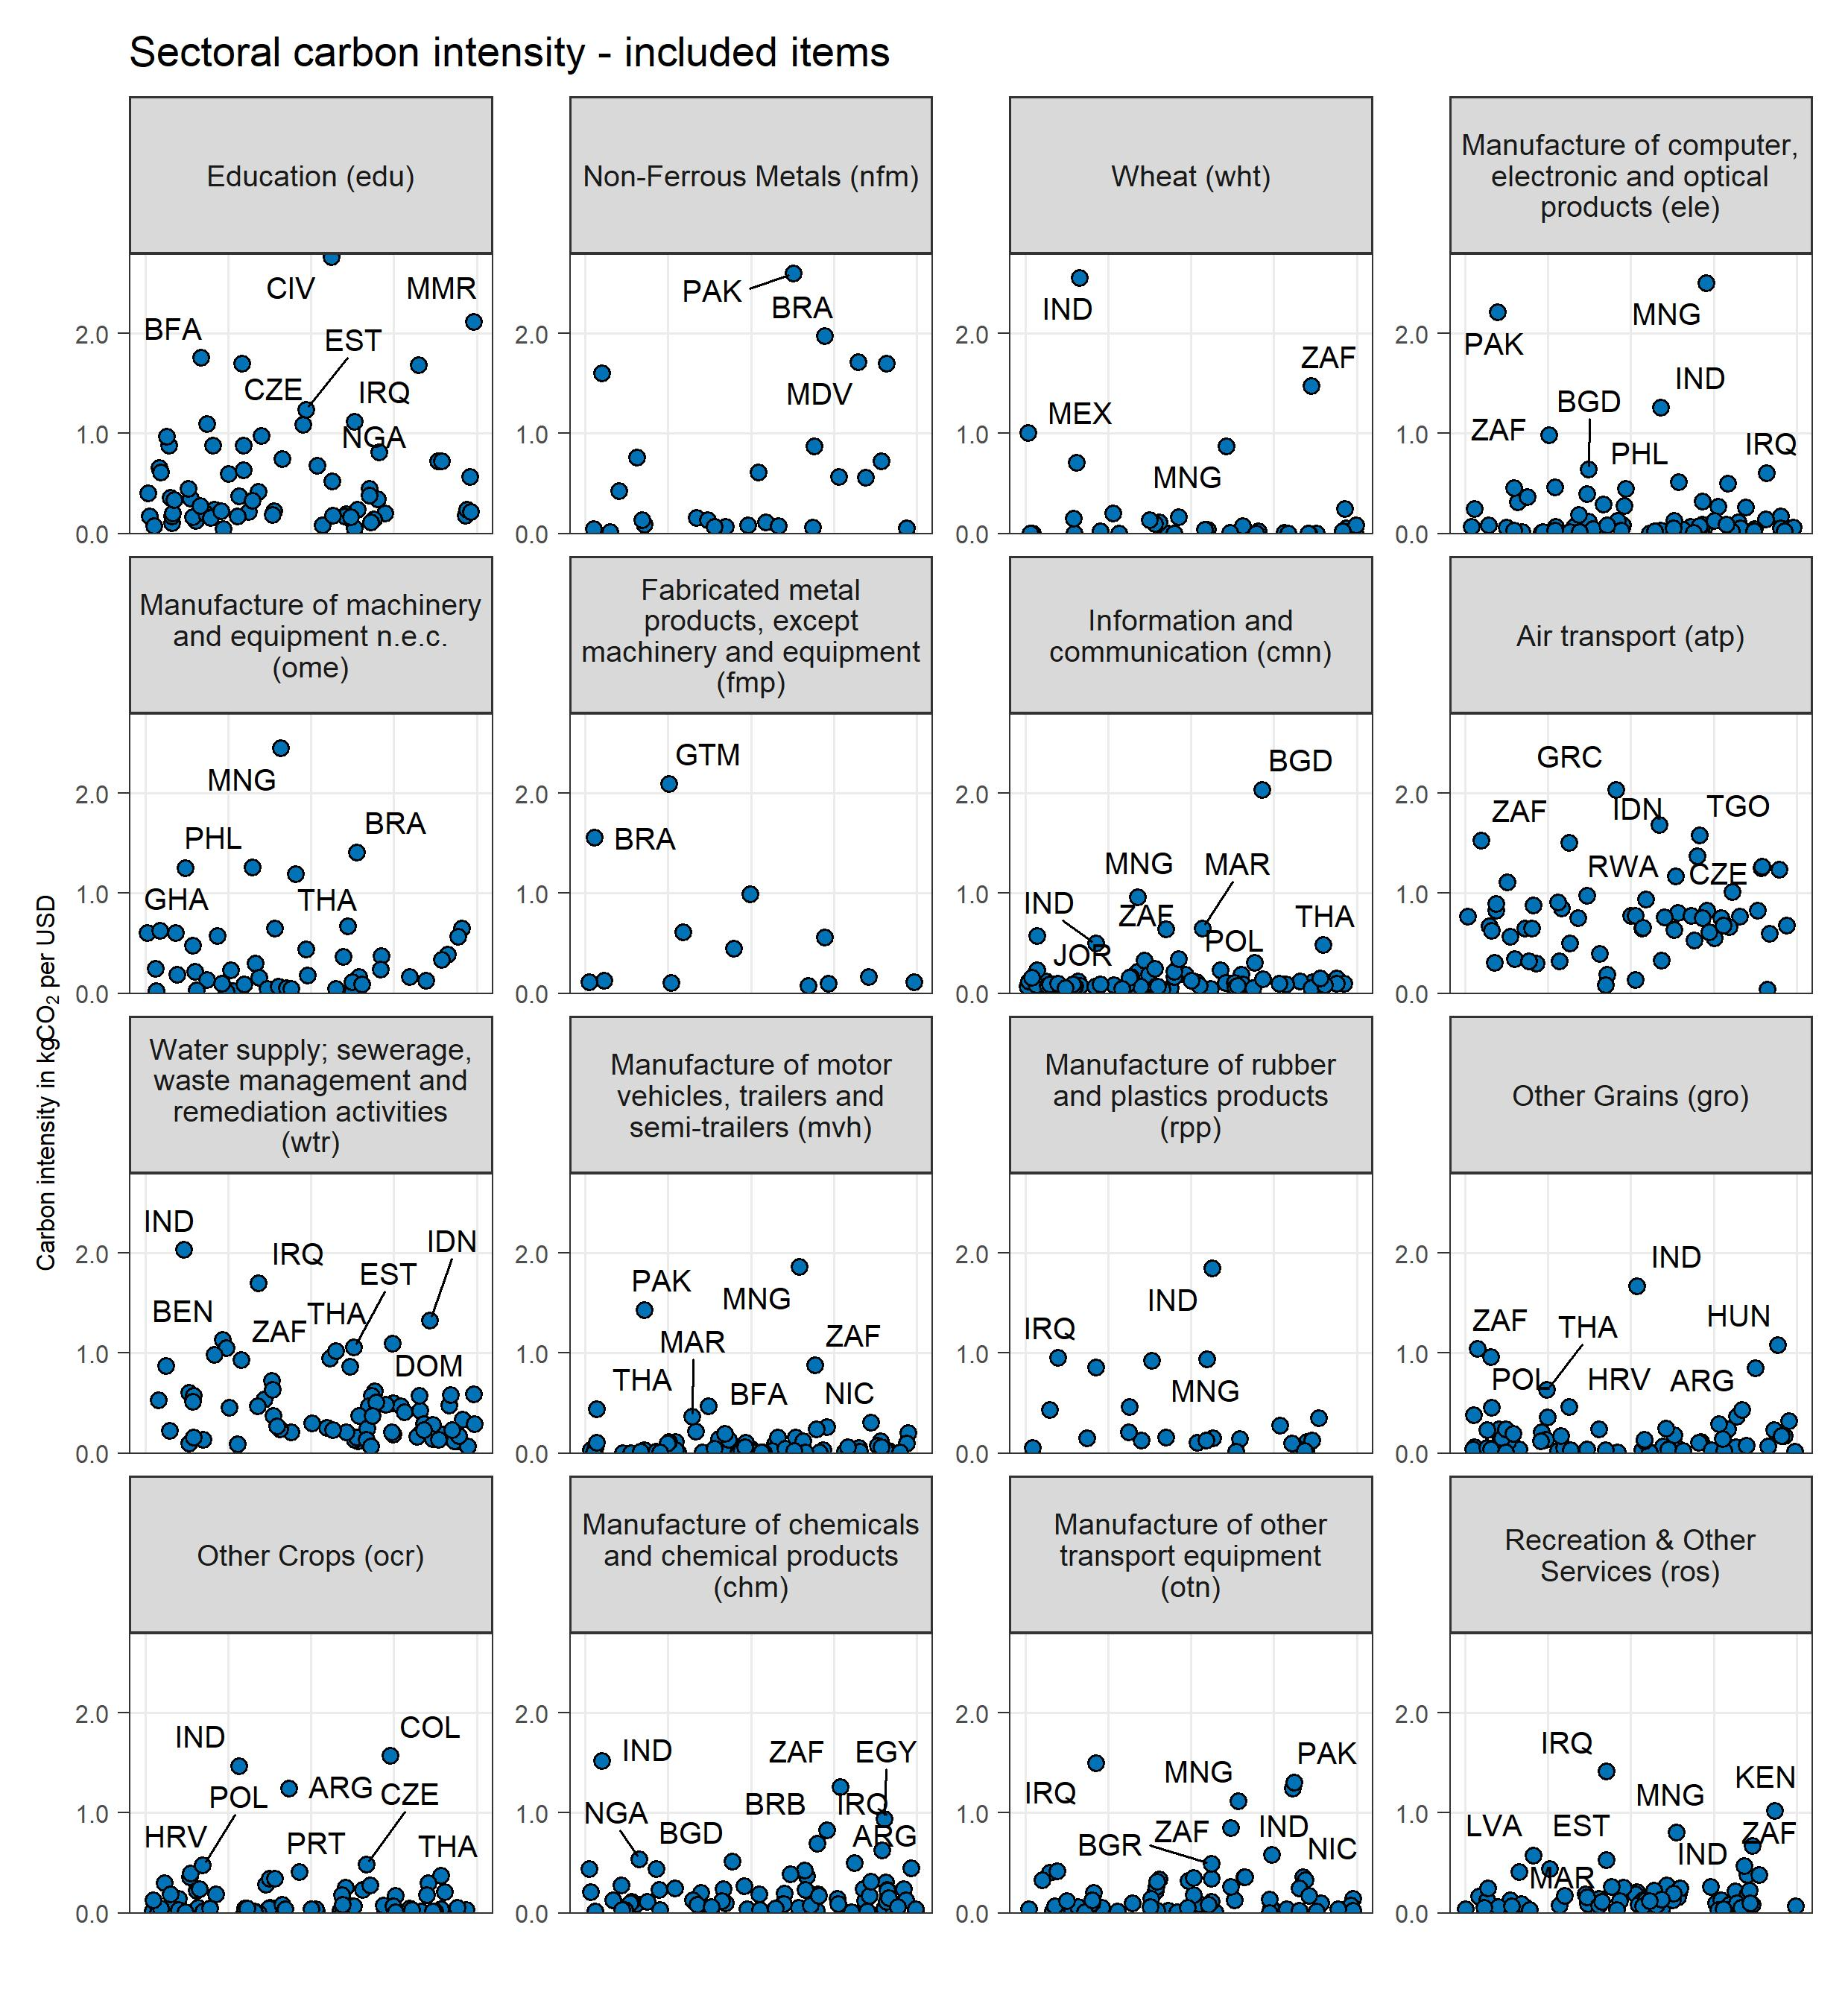
\includegraphics{Analysis_Carbon_Intensities_GTAP/Figure_2.1.1_C}
  \begin{subcaption}
    This figure displays...
  \end{subcaption}

\end{figure}

\clearpage

\begin{figure}[ht!]
  \centering
  \caption{Sectoral carbon intensities from GTAP - Part D} \label{fig:B4}
  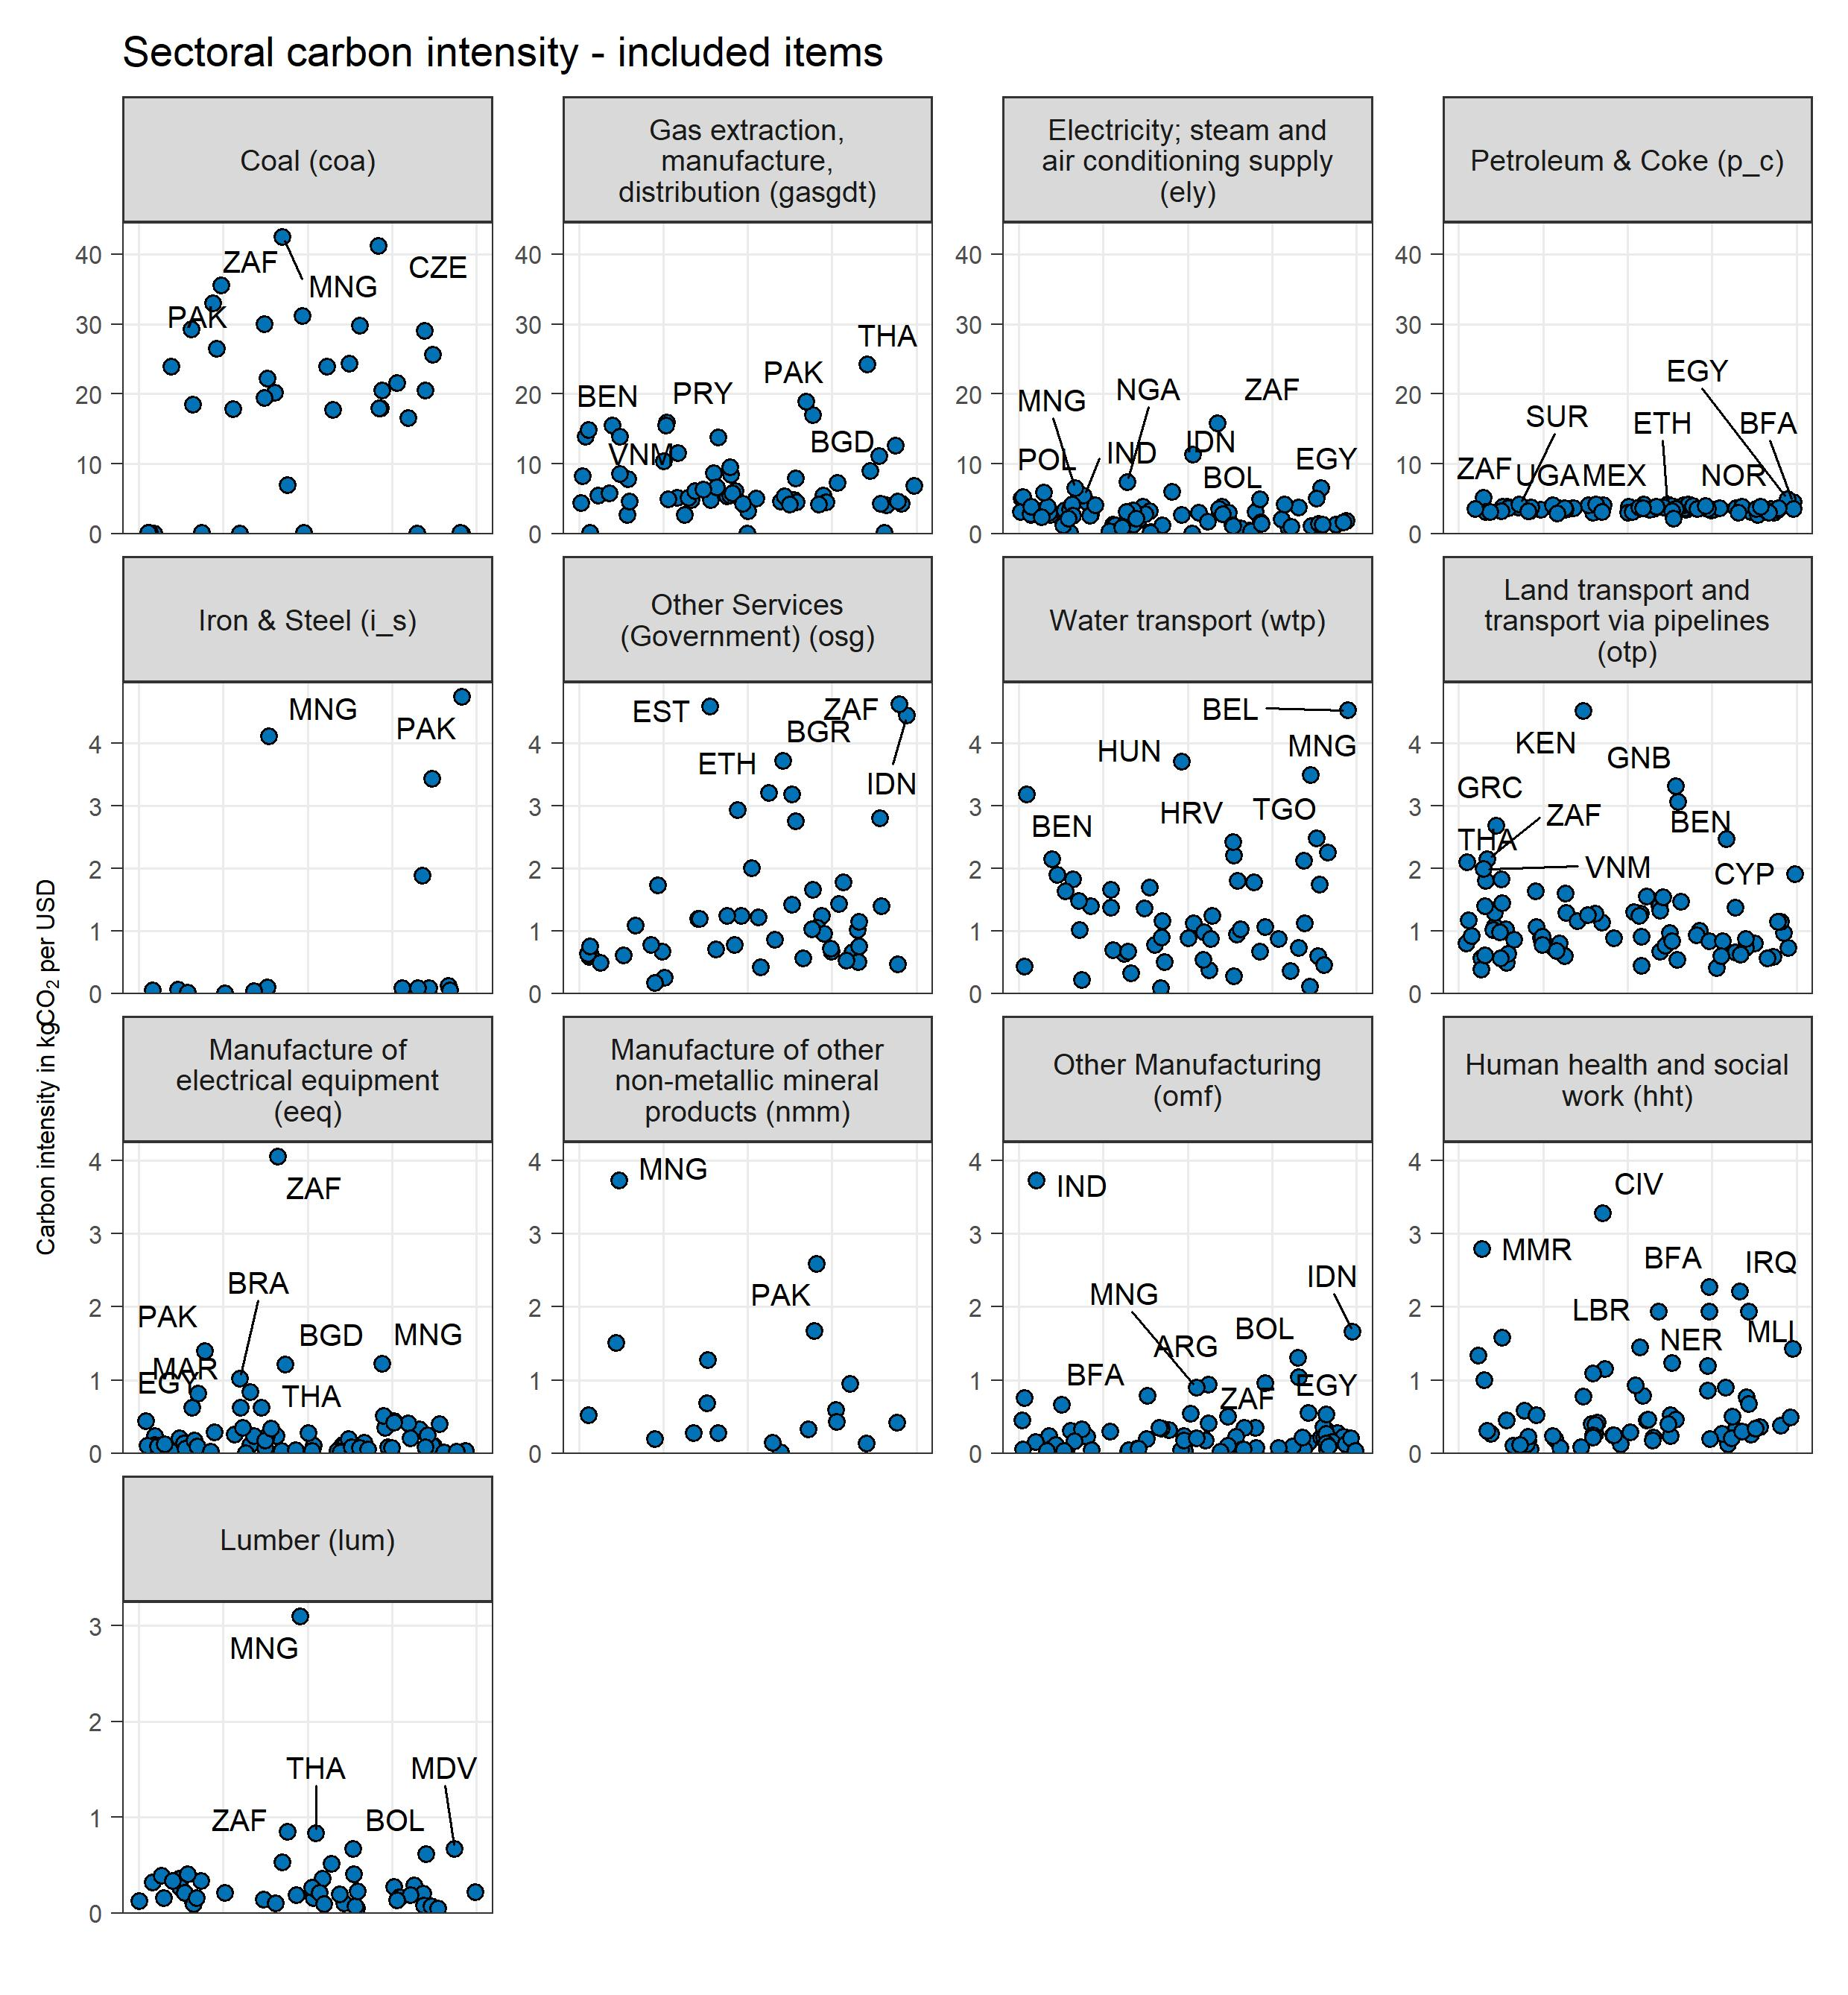
\includegraphics{Analysis_Carbon_Intensities_GTAP/Figure_2.1.1_D}
  \begin{subcaption}
    This figure displays...
  \end{subcaption}

\end{figure}

\clearpage

% Carbon intensity of consumption over total household expenditures

\begin{figure}[ht!]
  \centering
  \caption{Carbon intensity of consumption over total household expenditures - Part A} \label{fig:C1}
  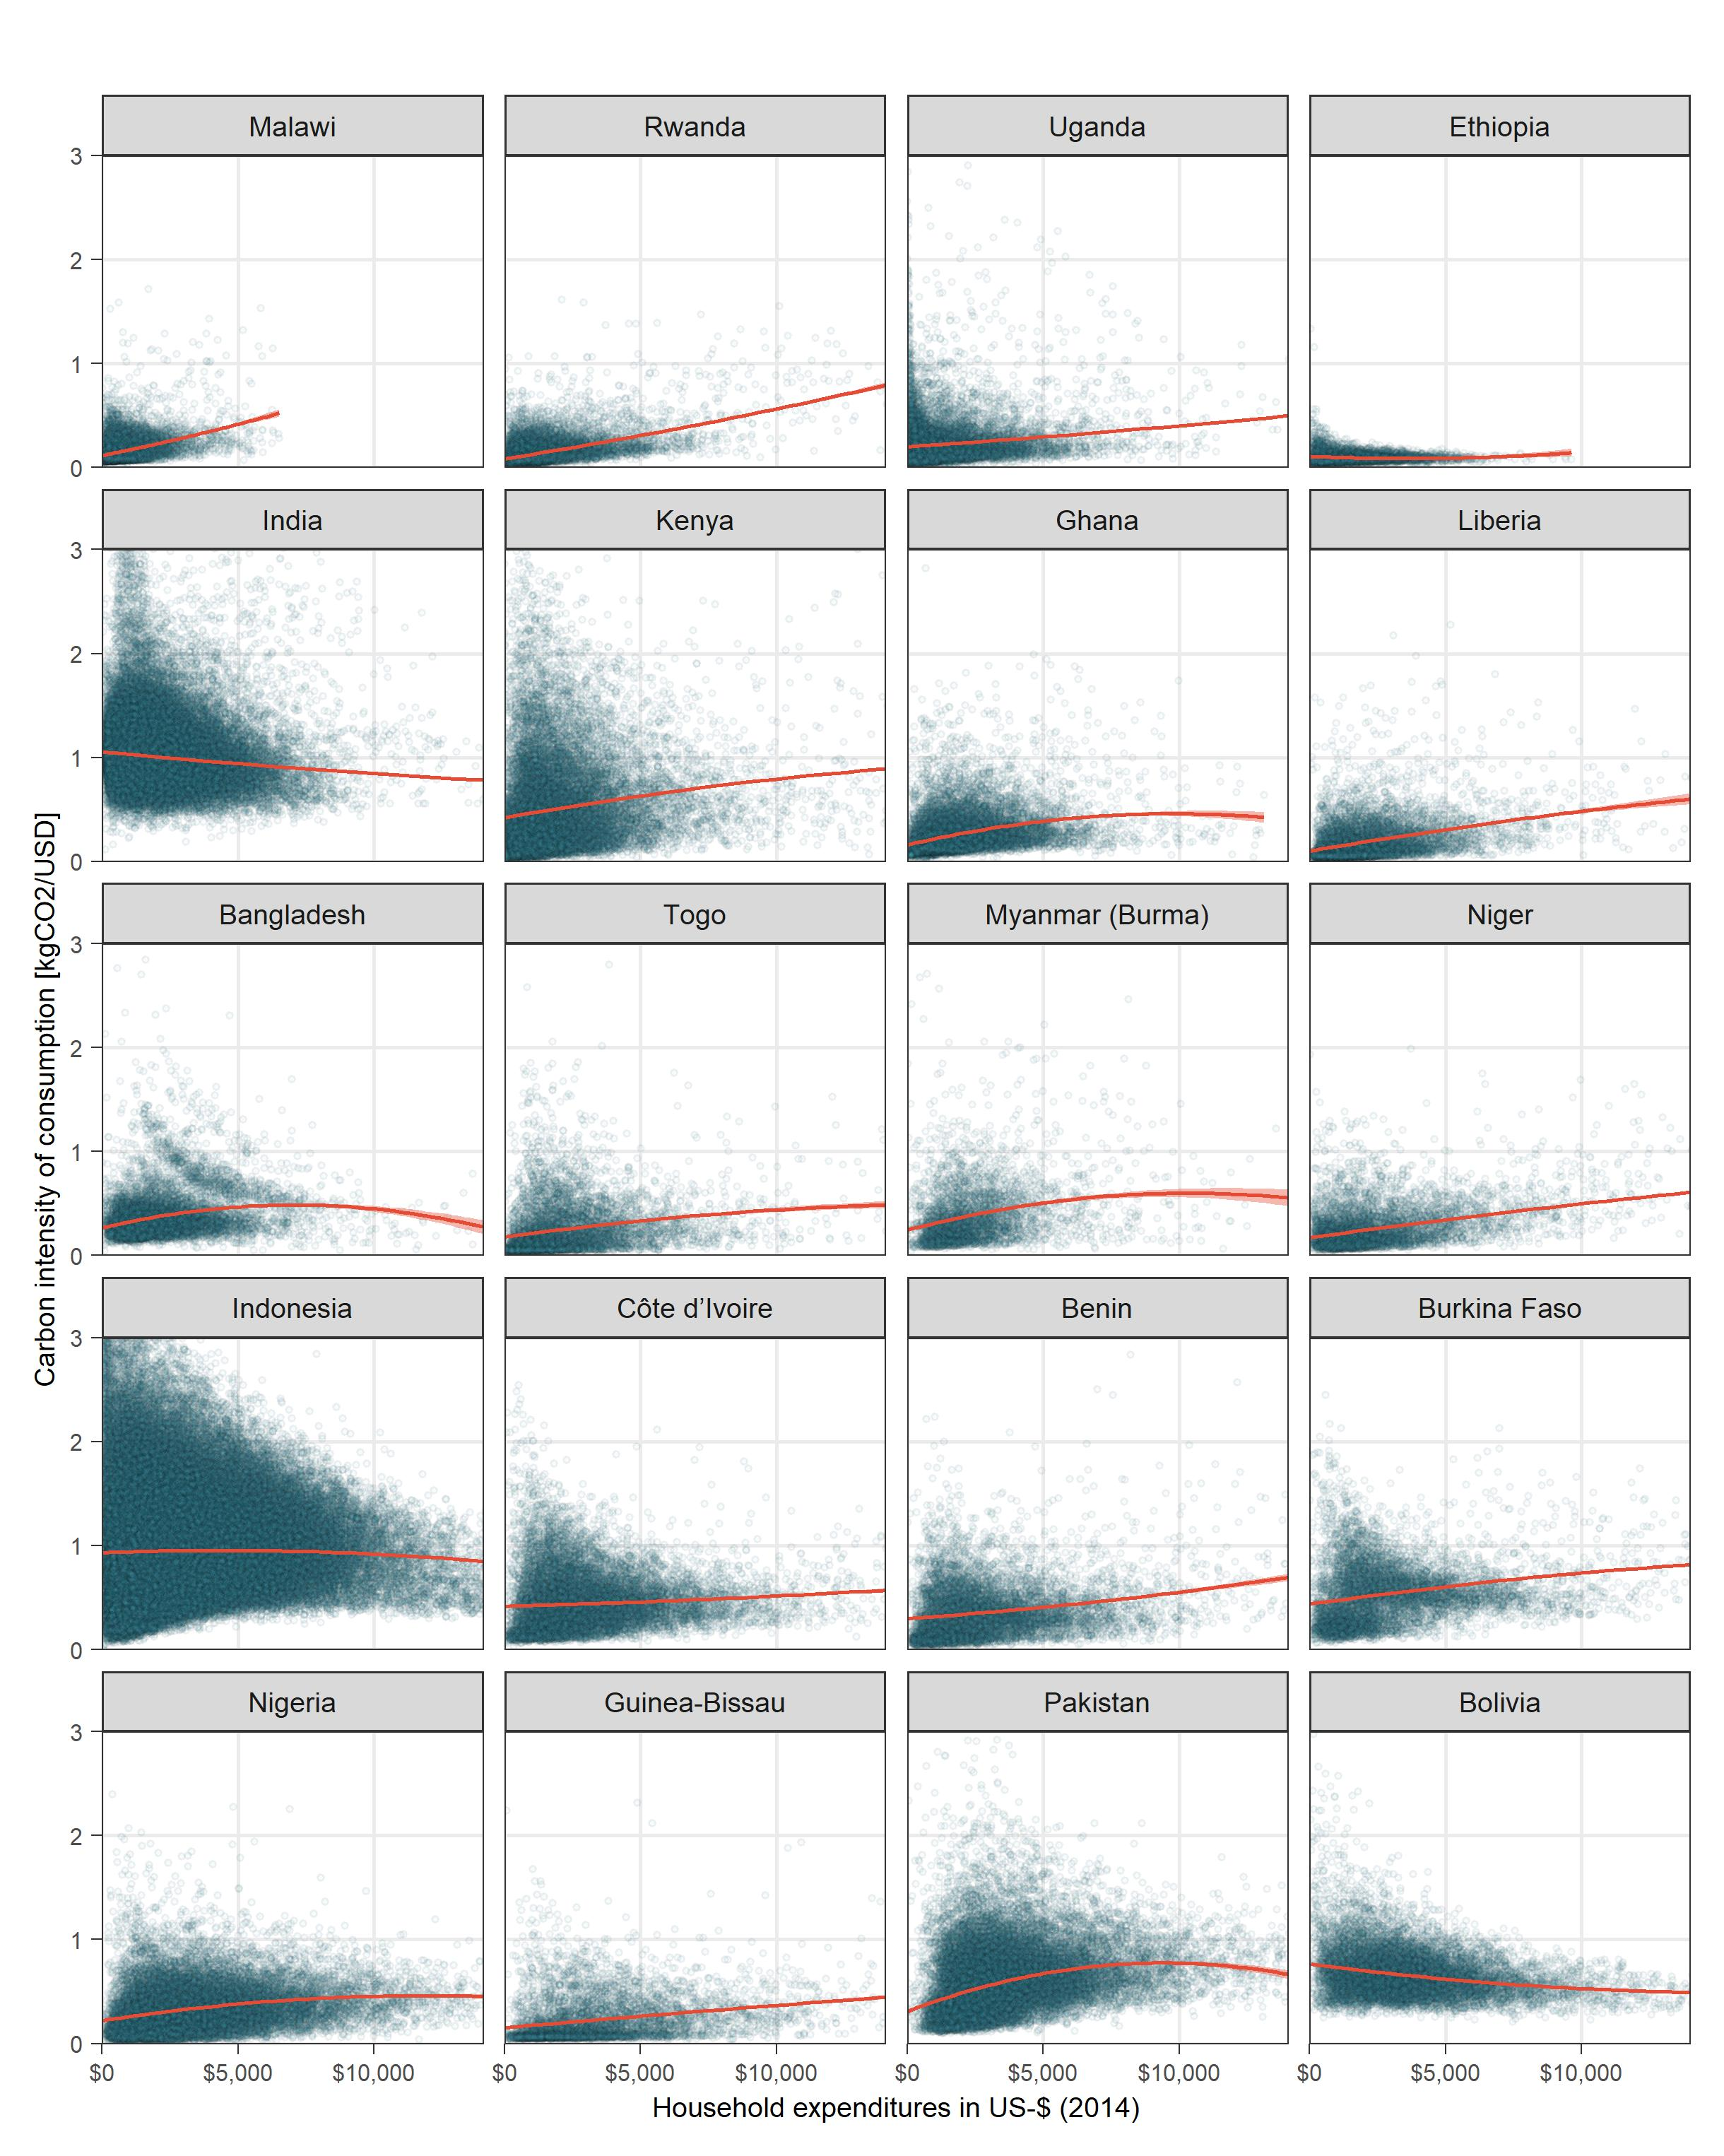
\includegraphics{Analysis_Carbon_Intensity_Curve/All_Panel_A}
  \begin{subcaption}
    This figure displays carbon intensity of aggregate consumption (in $kgCO_{2}/USD$) over total household expenditures in USD for 20 countries in our sample. Household expenditures are inflated (or deflated) to 2014. Points represent single households. The red line represents a fitted curve for a quadratic OLS-regression including a 95\%-confidence interval.
  \end{subcaption}

\end{figure}

\clearpage

\begin{figure}[ht!]
  \centering
  \caption{Carbon intensity of consumption over total household expenditures - Part B} \label{fig:C2}
  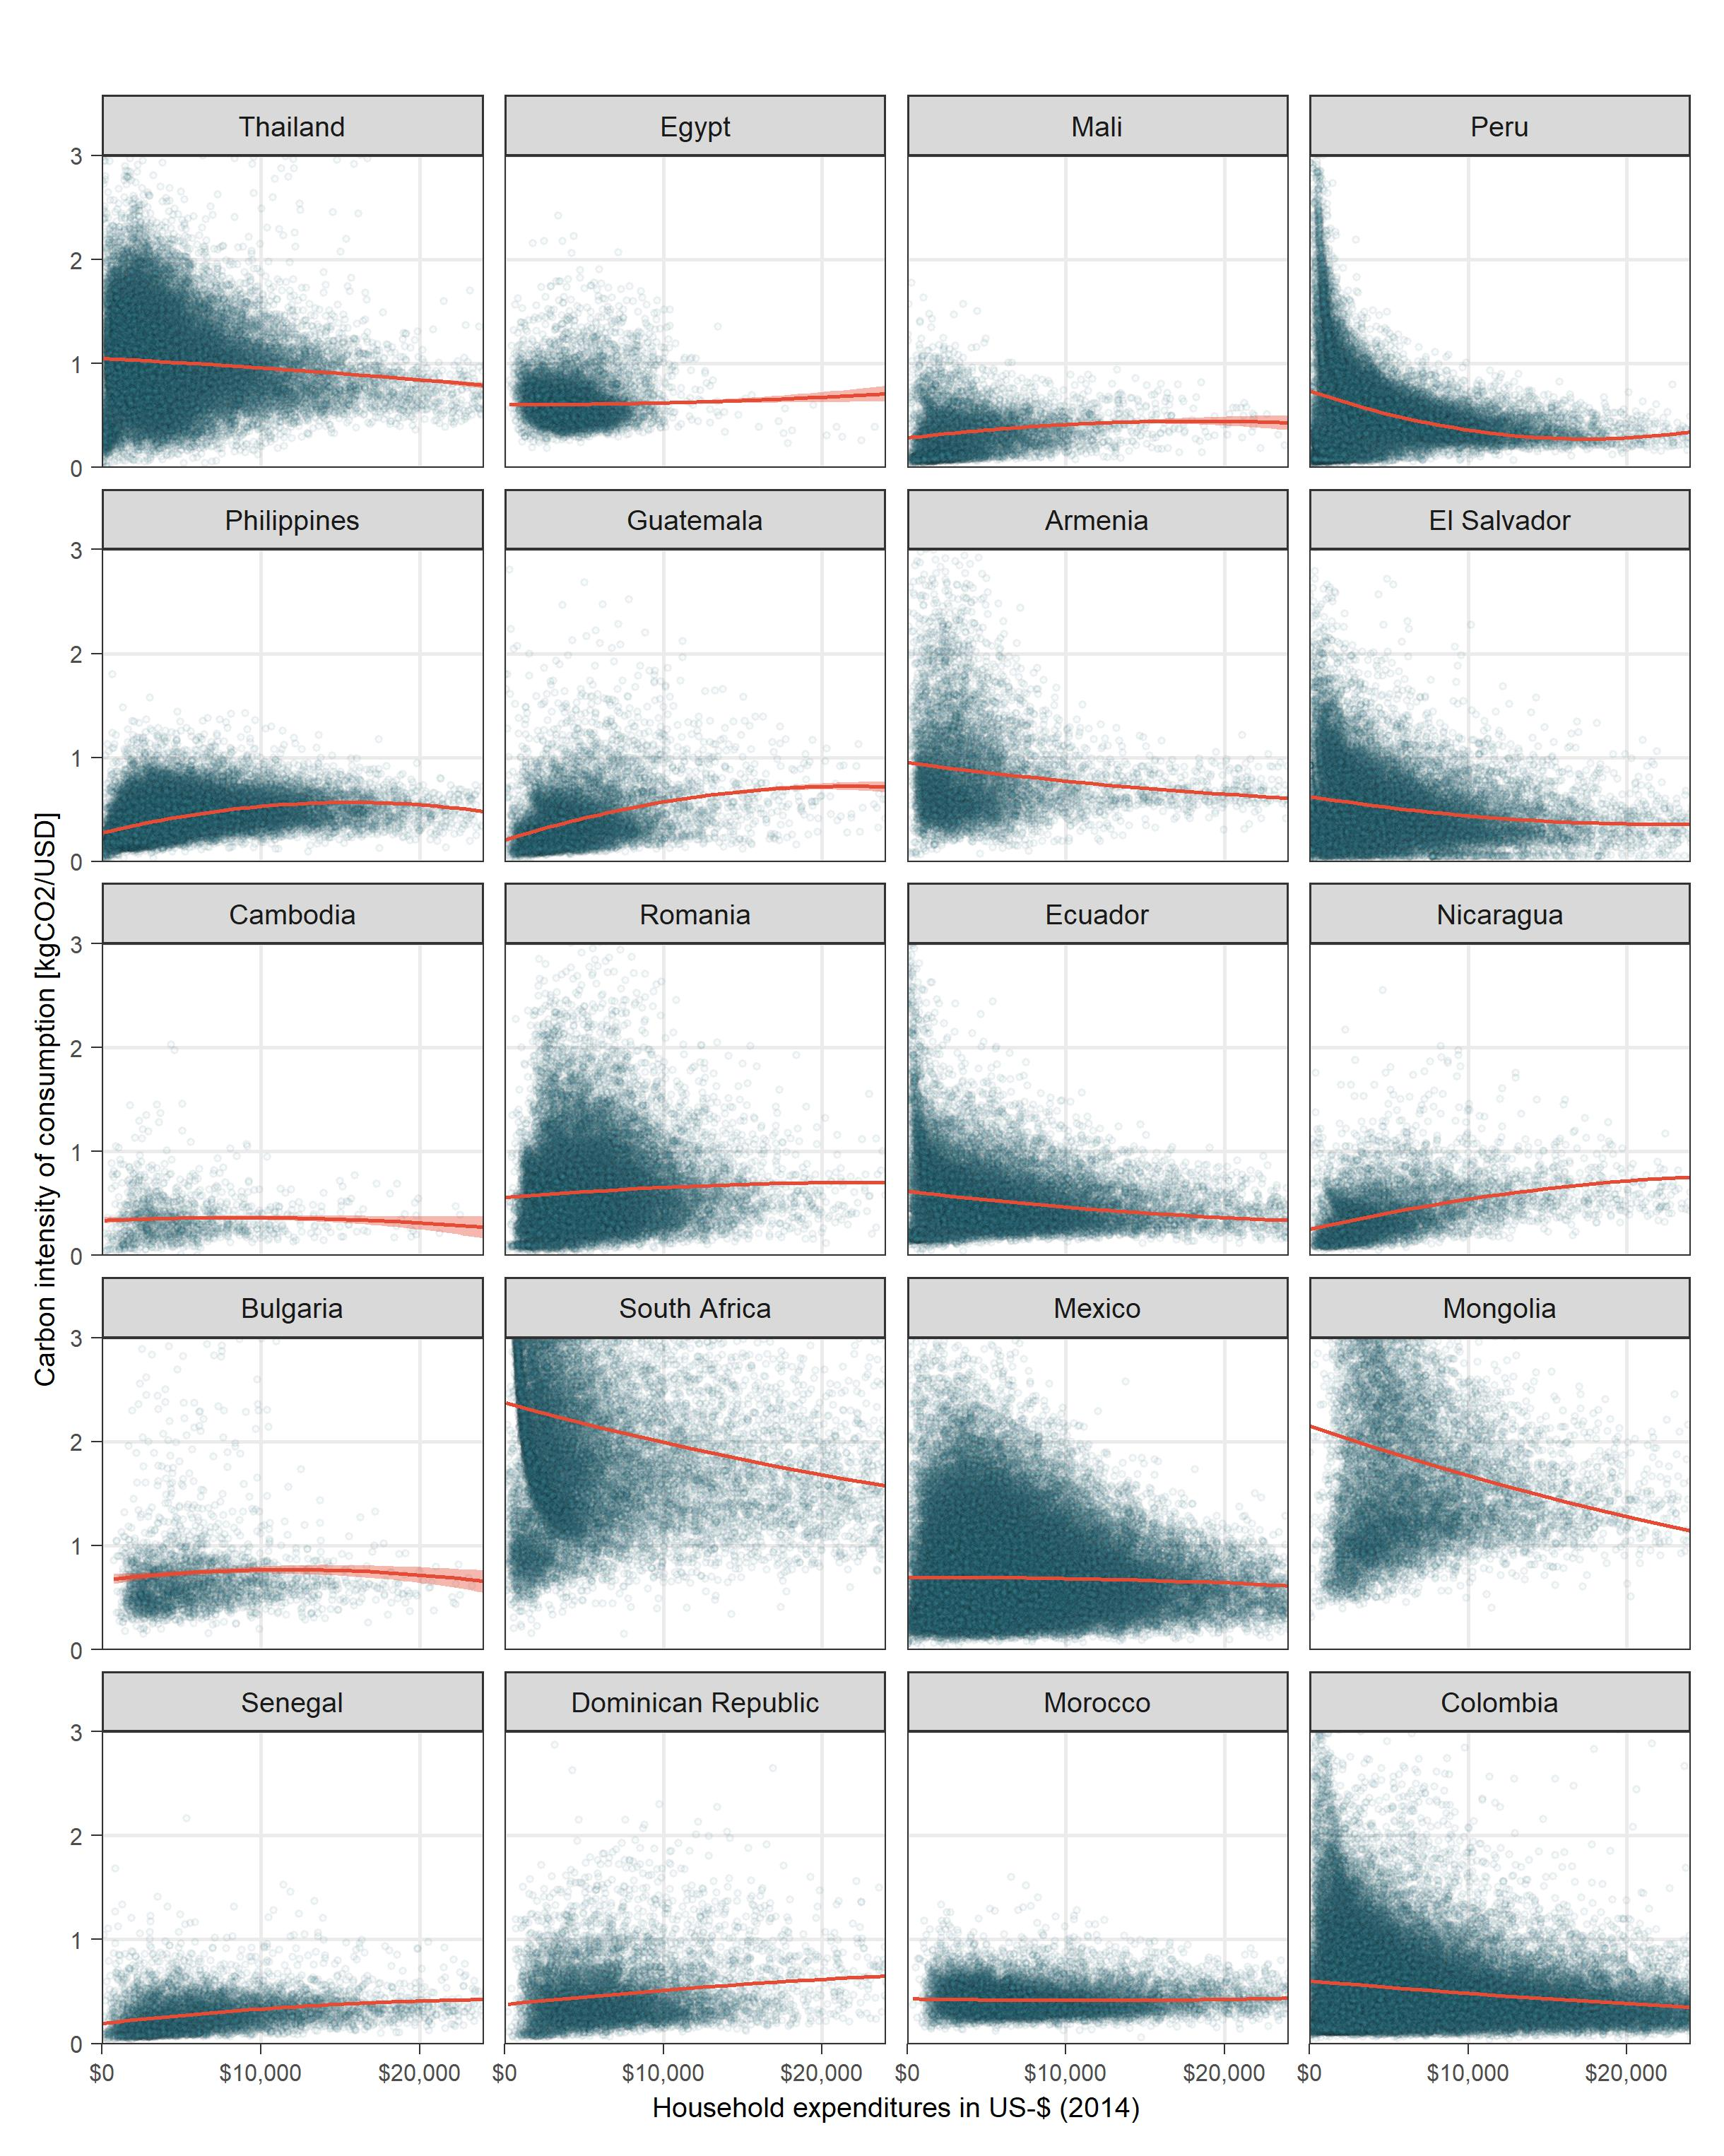
\includegraphics{Analysis_Carbon_Intensity_Curve/All_Panel_B}
  \begin{subcaption}
    This figure displays carbon intensity of aggregate consumption (in $kgCO_{2}/USD$) over total household expenditures in USD for 20 countries in our sample. Household expenditures are inflated (or deflated) to 2014. Points represent single households. The red line represents a fitted curve for a quadratic OLS-regression including a 95\%-confidence interval.
  \end{subcaption}

\end{figure}

\clearpage

\begin{figure}[ht!]
  \centering
  \caption{Carbon intensity of consumption over total household expenditures - Part C} \label{fig:C3}
  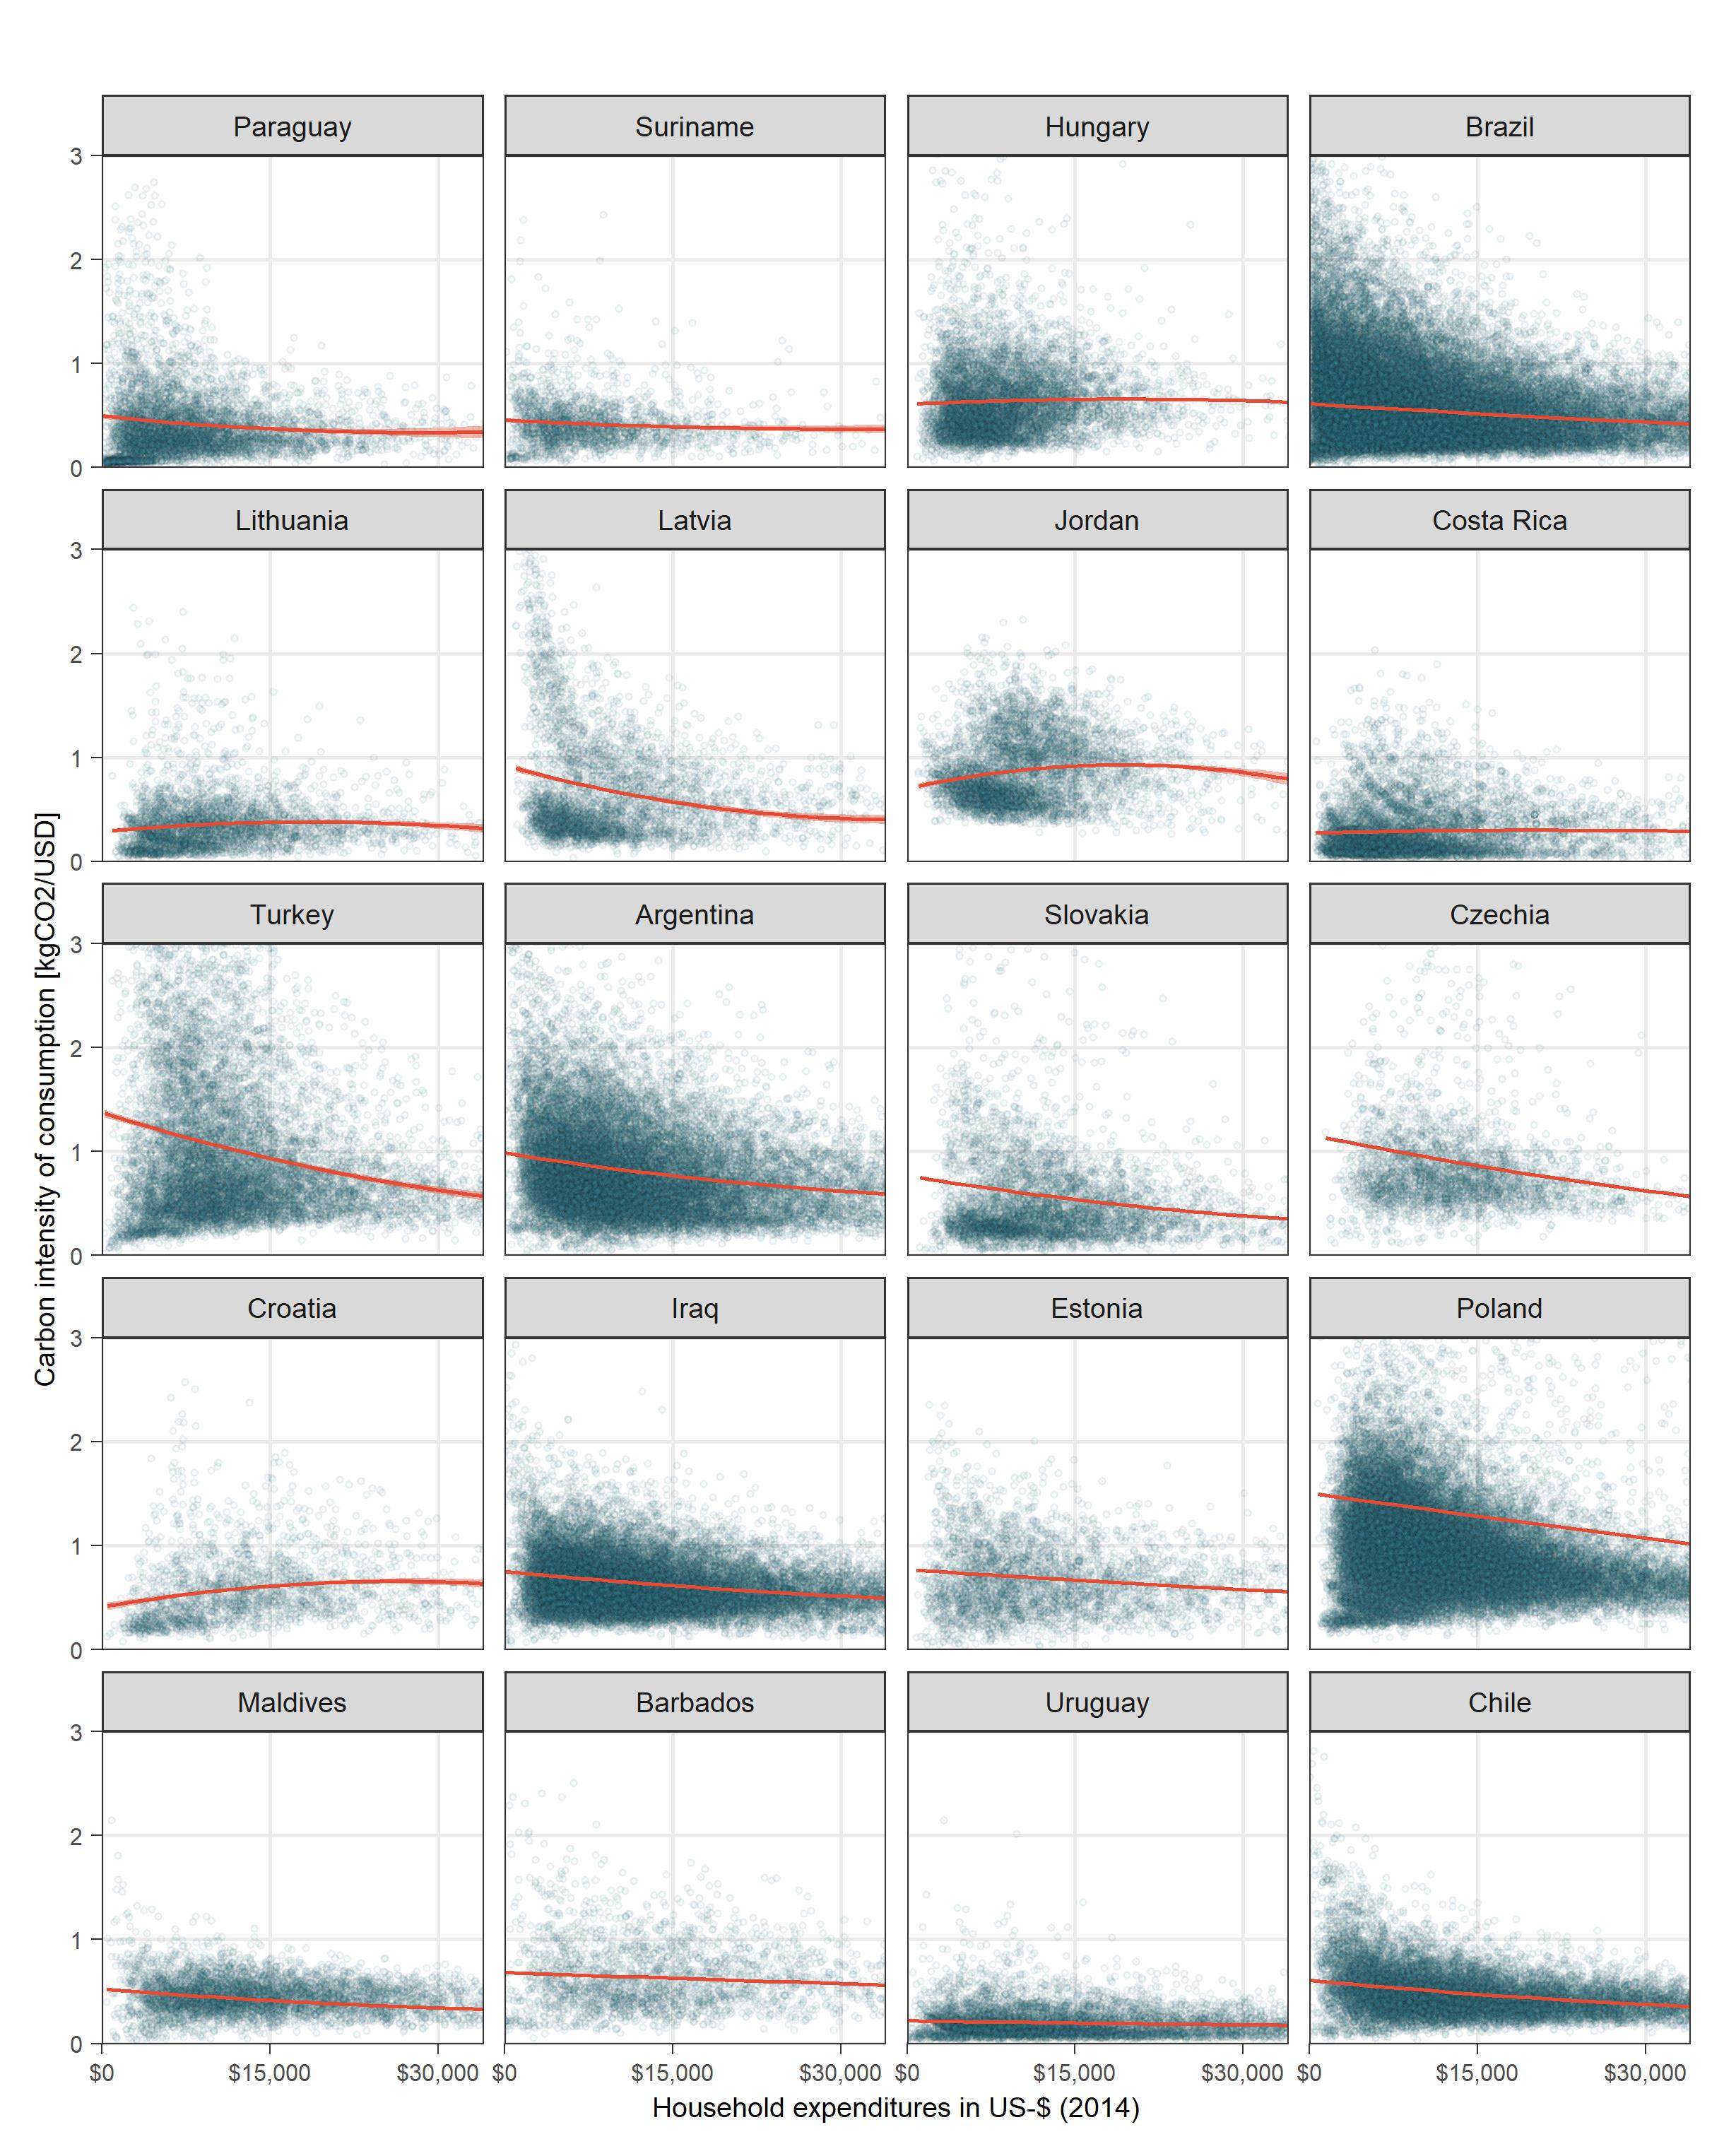
\includegraphics{Analysis_Carbon_Intensity_Curve/All_Panel_C}
  \begin{subcaption}
    This figure displays carbon intensity of aggregate consumption (in $kgCO_{2}/USD$) over total household expenditures in USD for 20 countries in our sample. Household expenditures are inflated (or deflated) to 2014. Points represent single households. The red line represents a fitted curve for a quadratic OLS-regression including a 95\%-confidence interval.
  \end{subcaption}

\end{figure}

\clearpage

\begin{figure}[ht!]
  \centering
  \caption{Carbon intensity of consumption over total household expenditures - Part D} \label{fig:C4}
  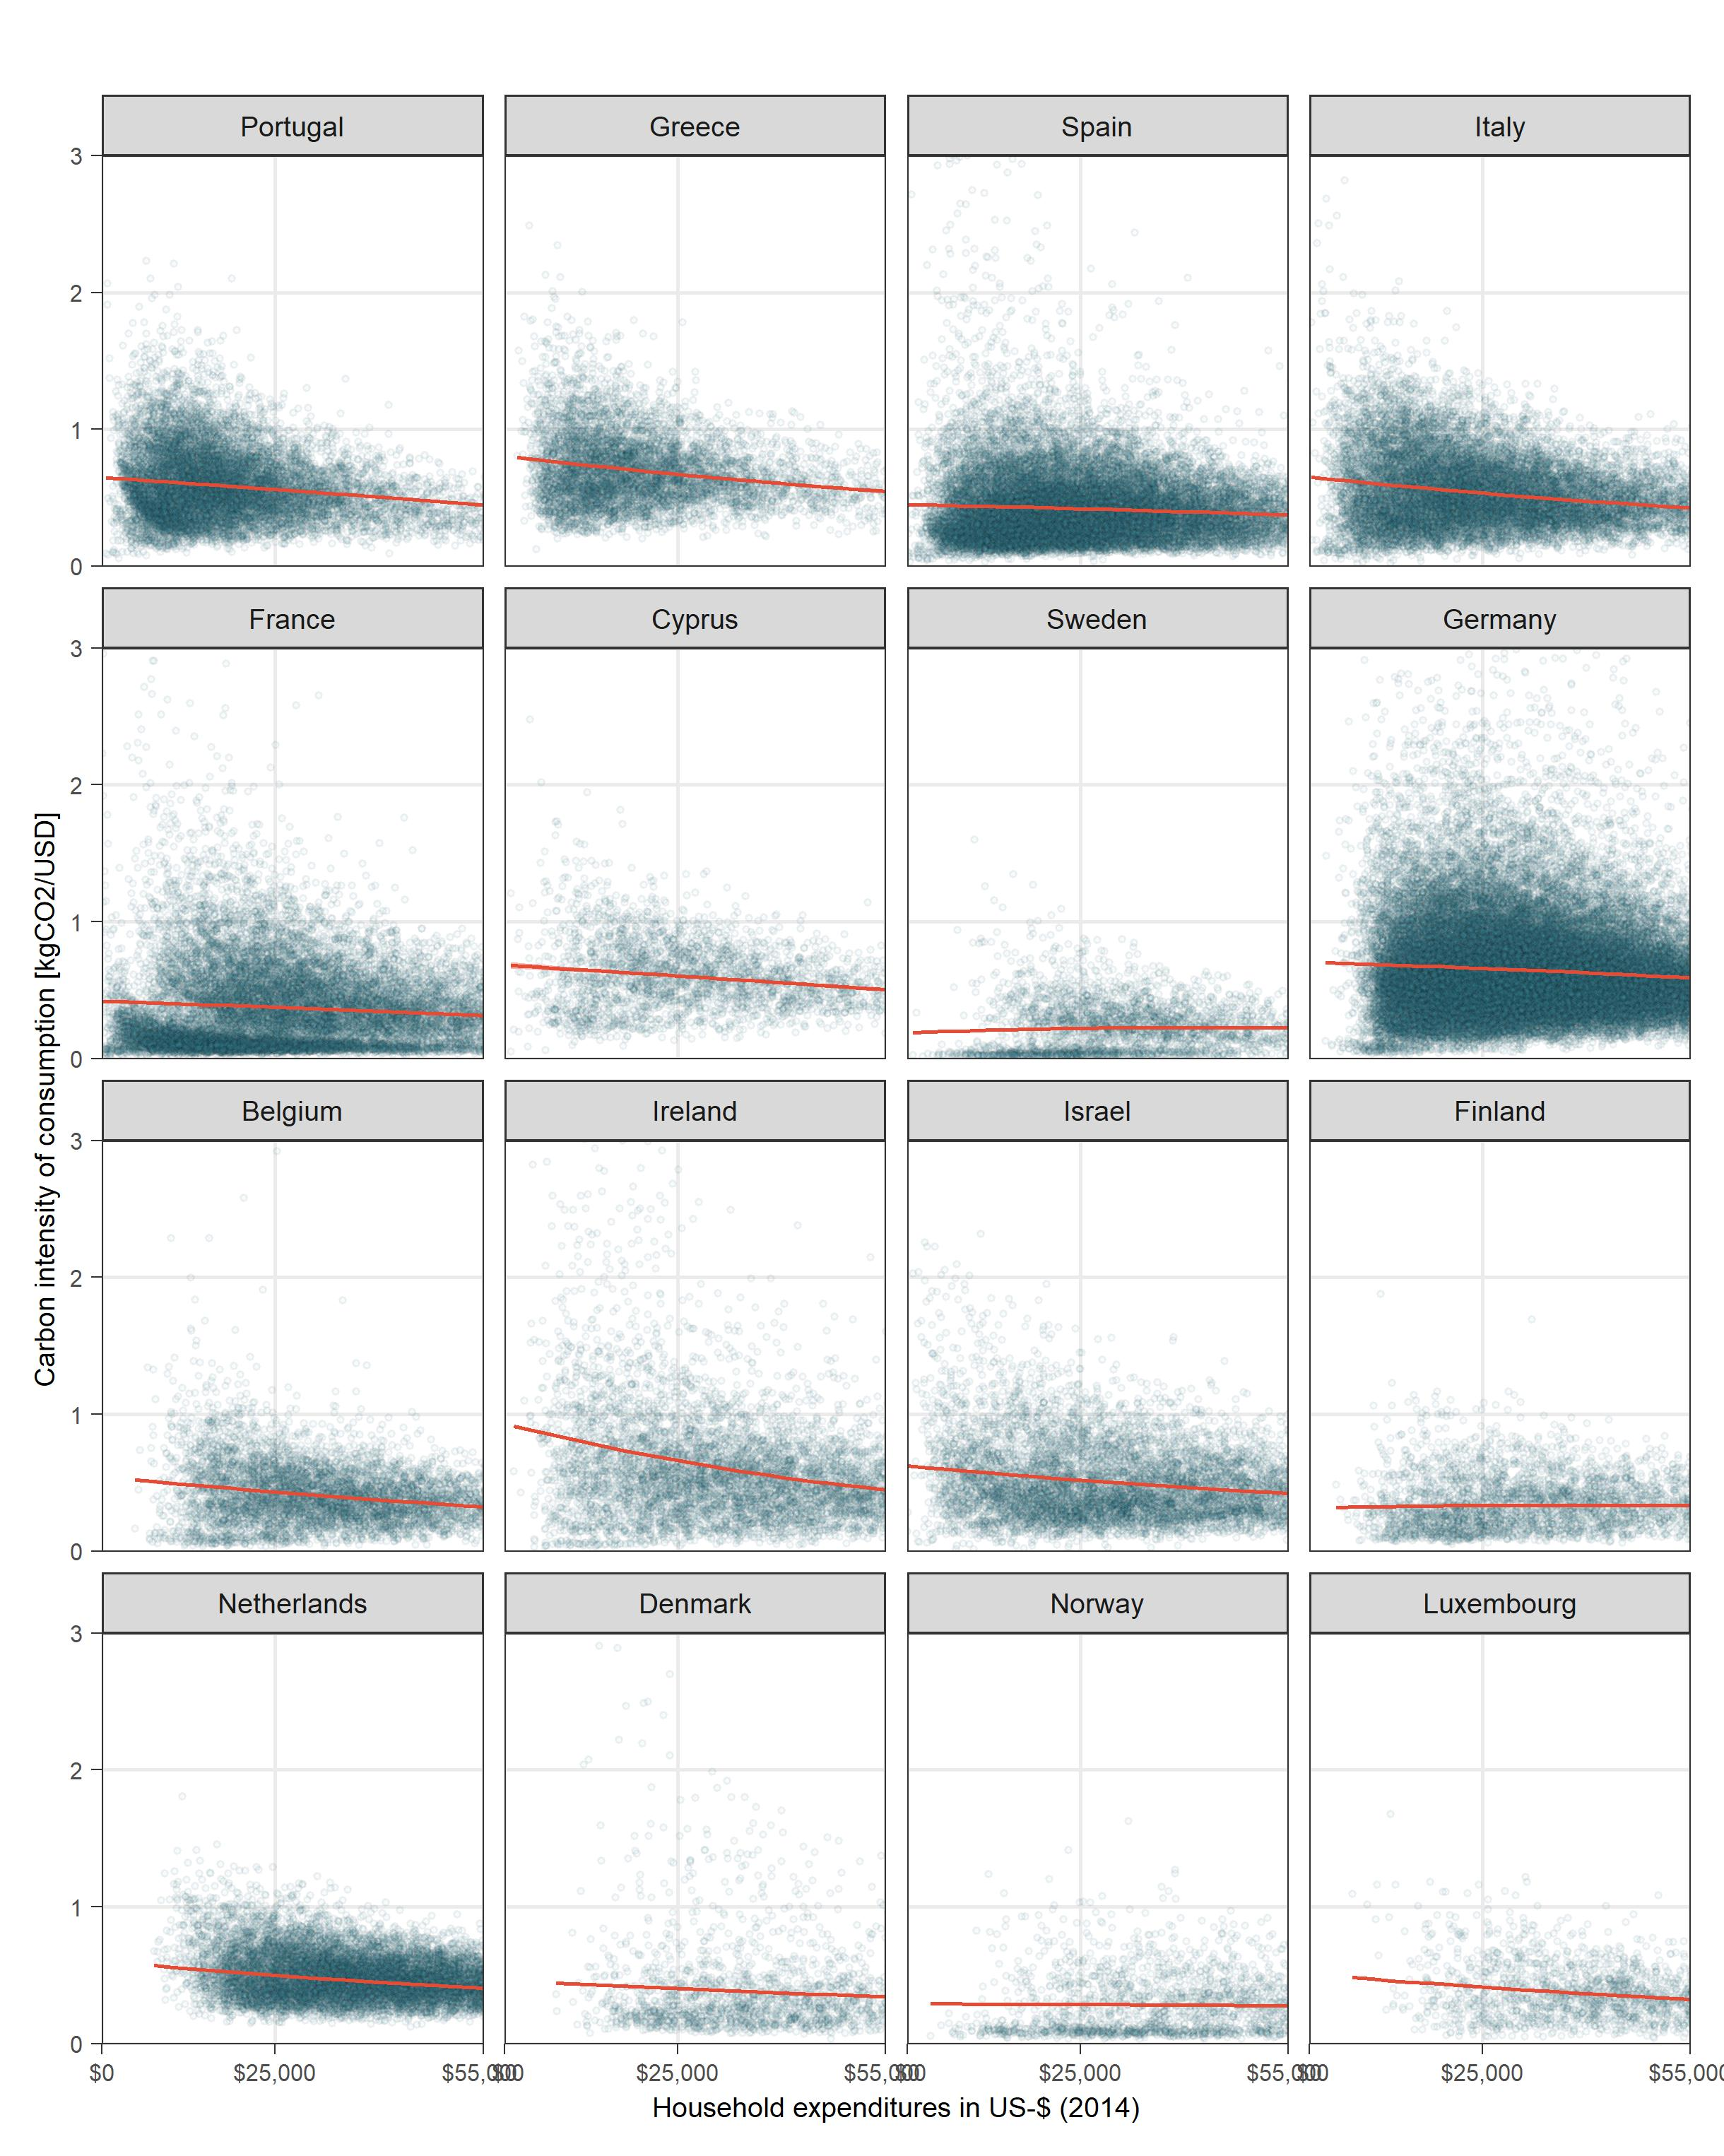
\includegraphics{Analysis_Carbon_Intensity_Curve/All_Panel_D}
  \begin{subcaption}
    This figure displays carbon intensity of aggregate consumption (in $kgCO_{2}/USD$) over total household expenditures in USD for 20 countries in our sample. Household expenditures are inflated (or deflated) to 2014. Points represent single households. The red line represents a fitted curve for a quadratic OLS-regression including a 95\%-confidence interval.
  \end{subcaption}

\end{figure}

\clearpage

% \begin{figure}[ht!]
%   \centering
%  \caption{Average marginal effects of car ownership} \label{fig:D1_Car}
%   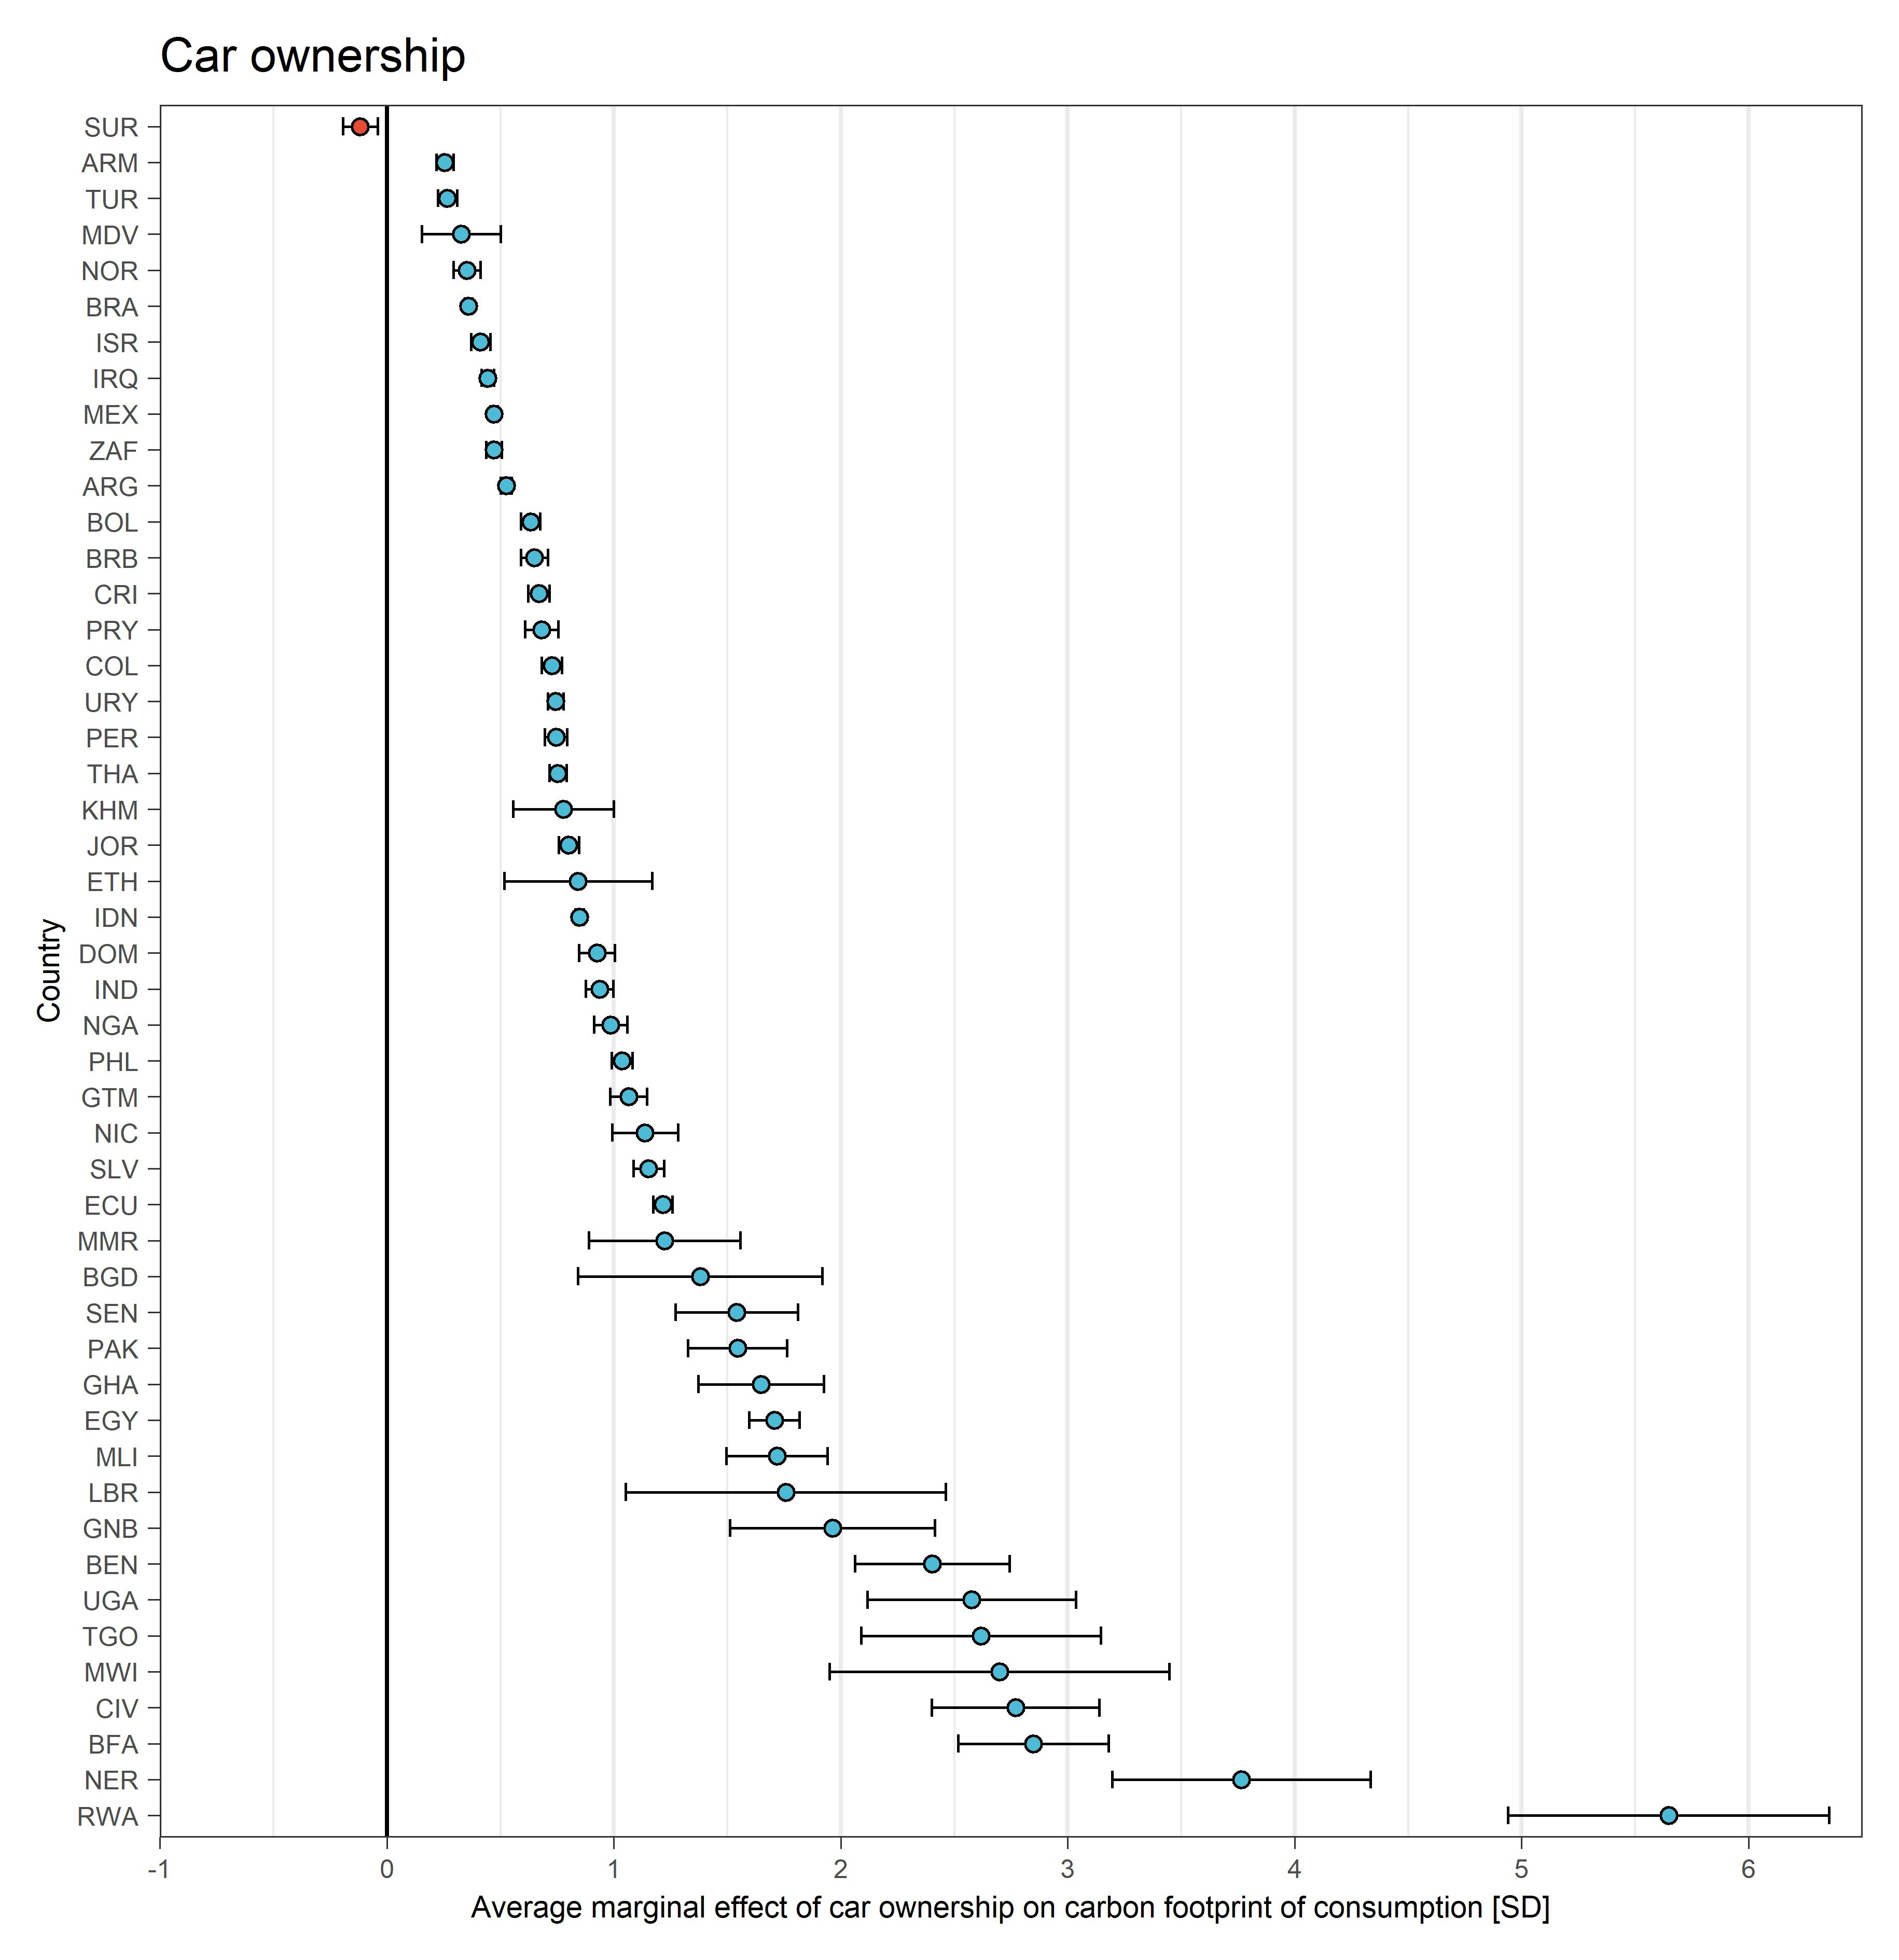
\includegraphics{Analysis_OLS_ME_Carbon_Footprint/AME_OLS_FP_car.01}
%   \begin{subcaption}
%     This figure displays ...
%   \end{subcaption}

% \end{figure}

% \clearpage

% \begin{figure}[ht!]
%   \centering
%  \caption{Average marginal effects of electricity access} \label{fig:D2_Electricity}
%   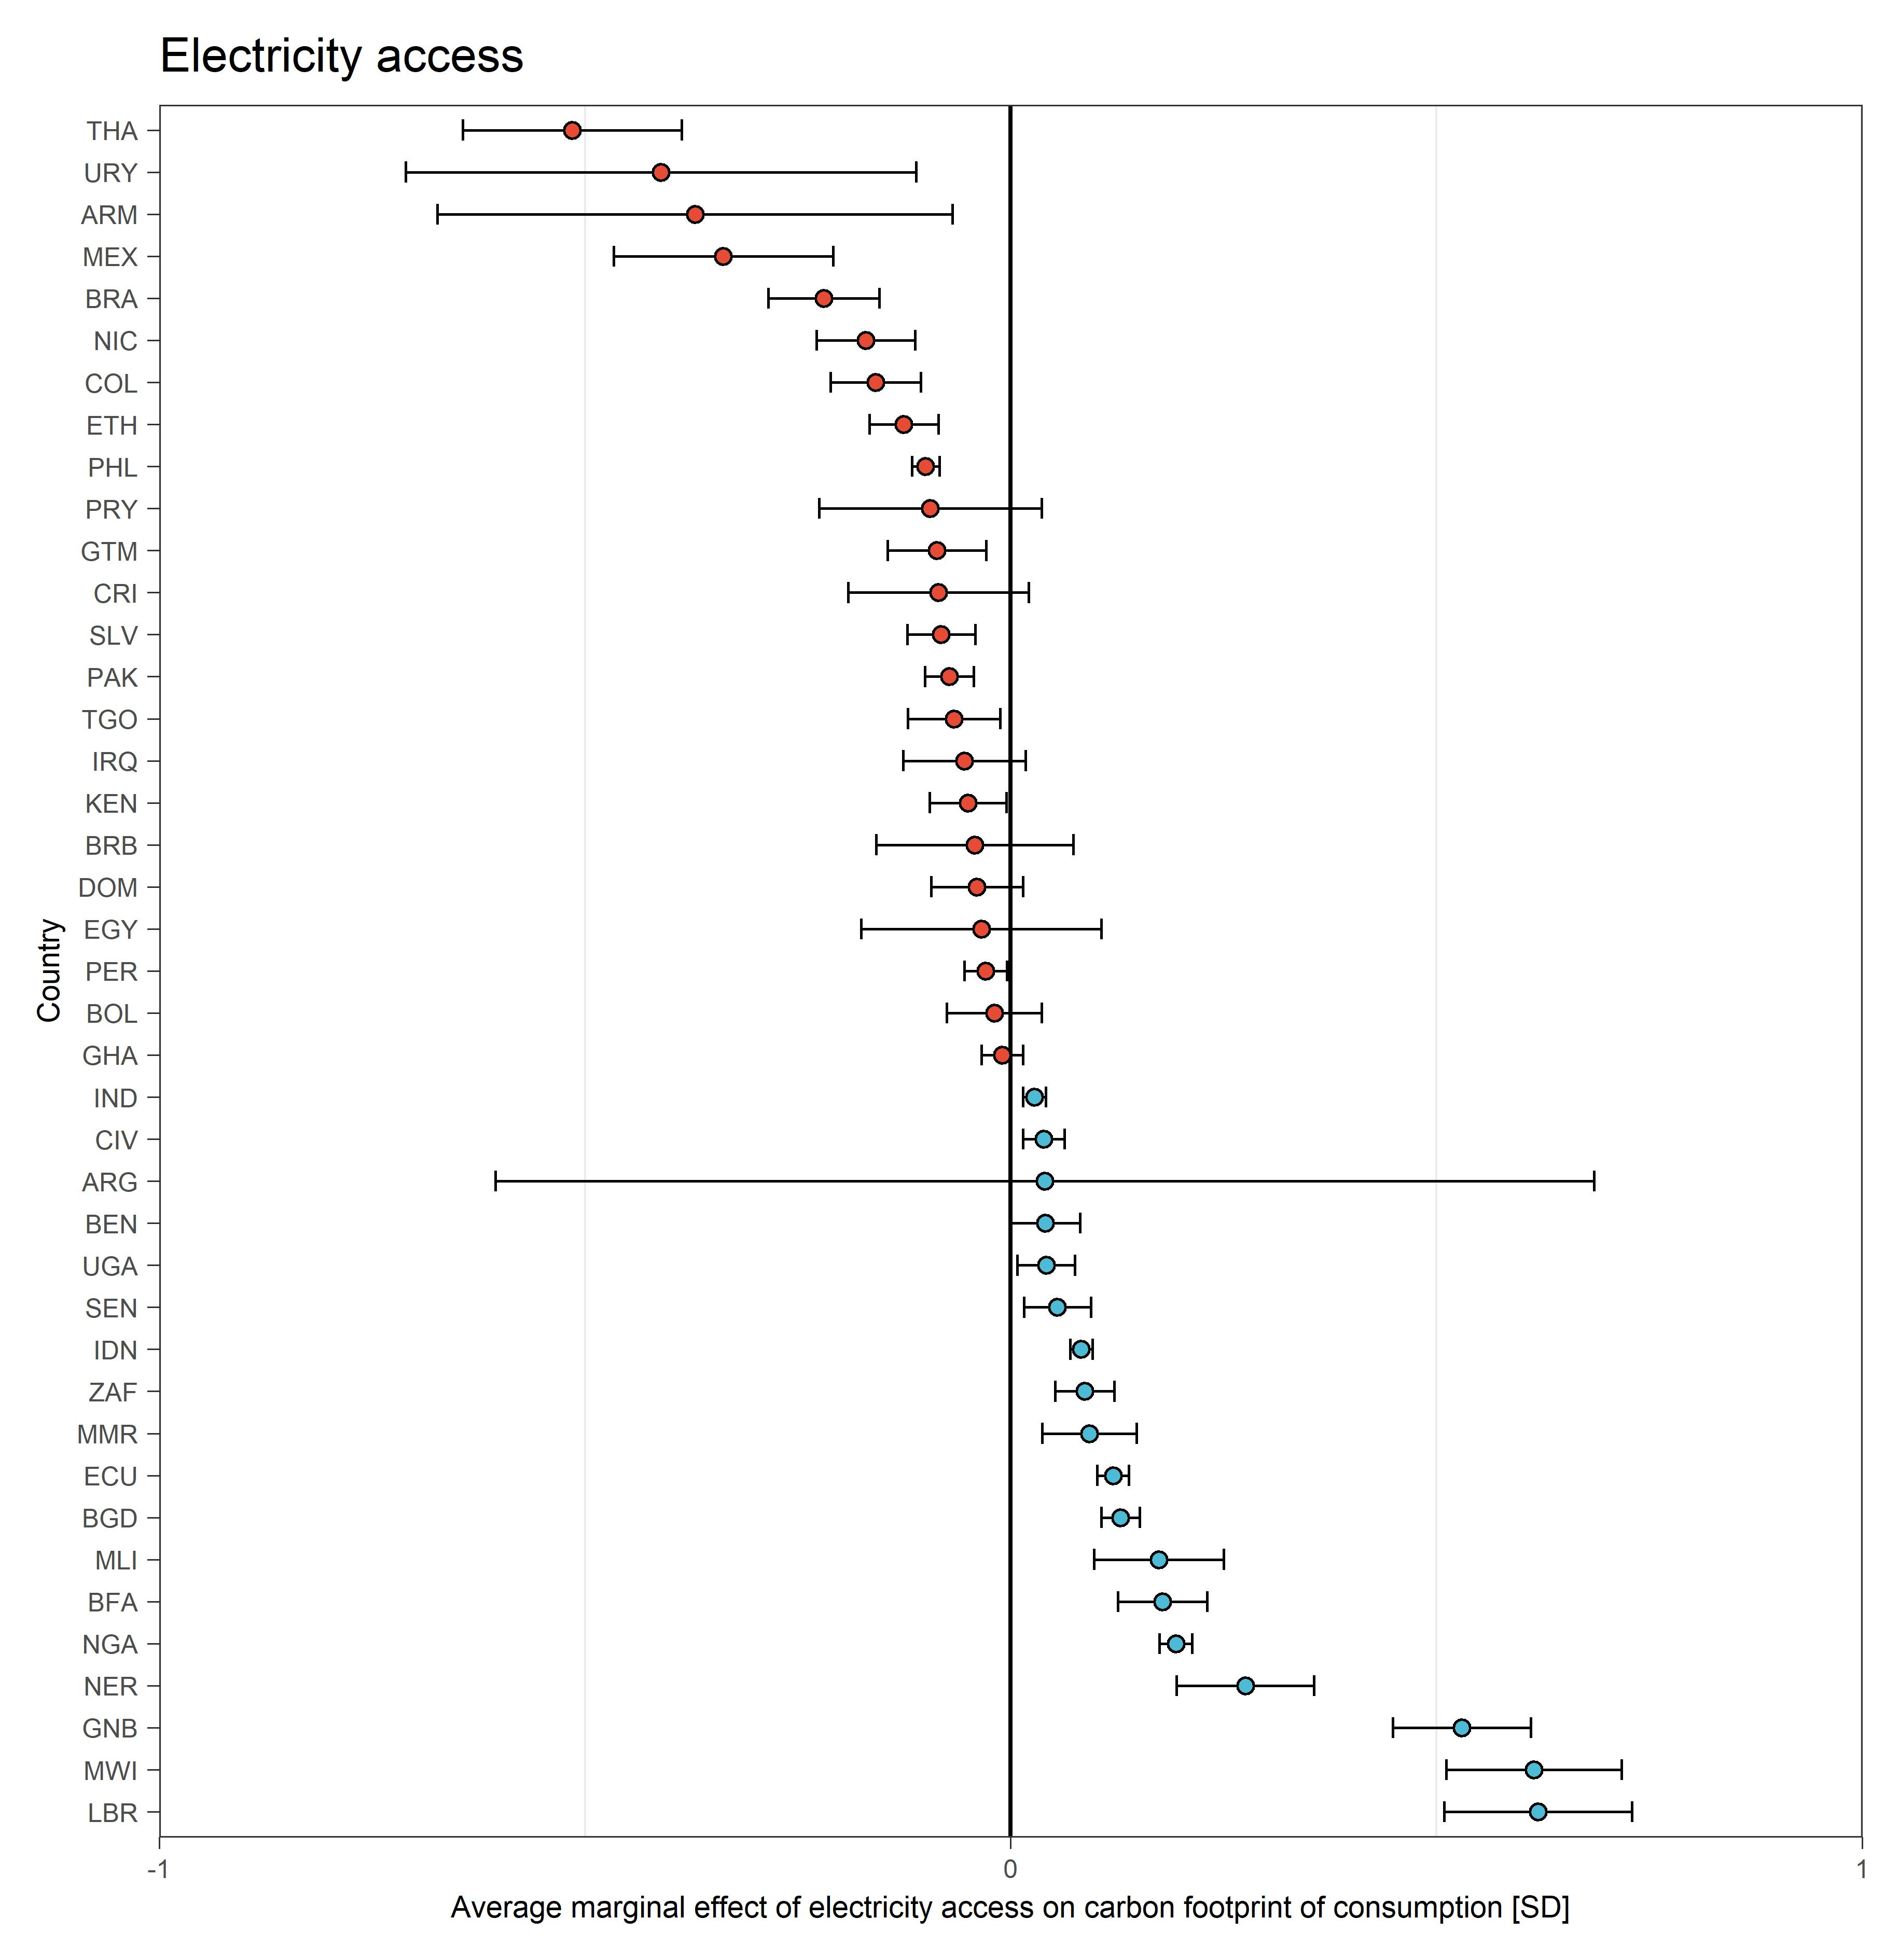
\includegraphics{Analysis_OLS_ME_Carbon_Footprint/AME_OLS_FP_electricity.access}
%   \begin{subcaption}
%     This figure displays ...
%   \end{subcaption}

% \end{figure}

% \clearpage

% \begin{figure}[ht!]
%   \centering
%  \caption{Average marginal effects of household size} \label{fig:D3_Size}
%   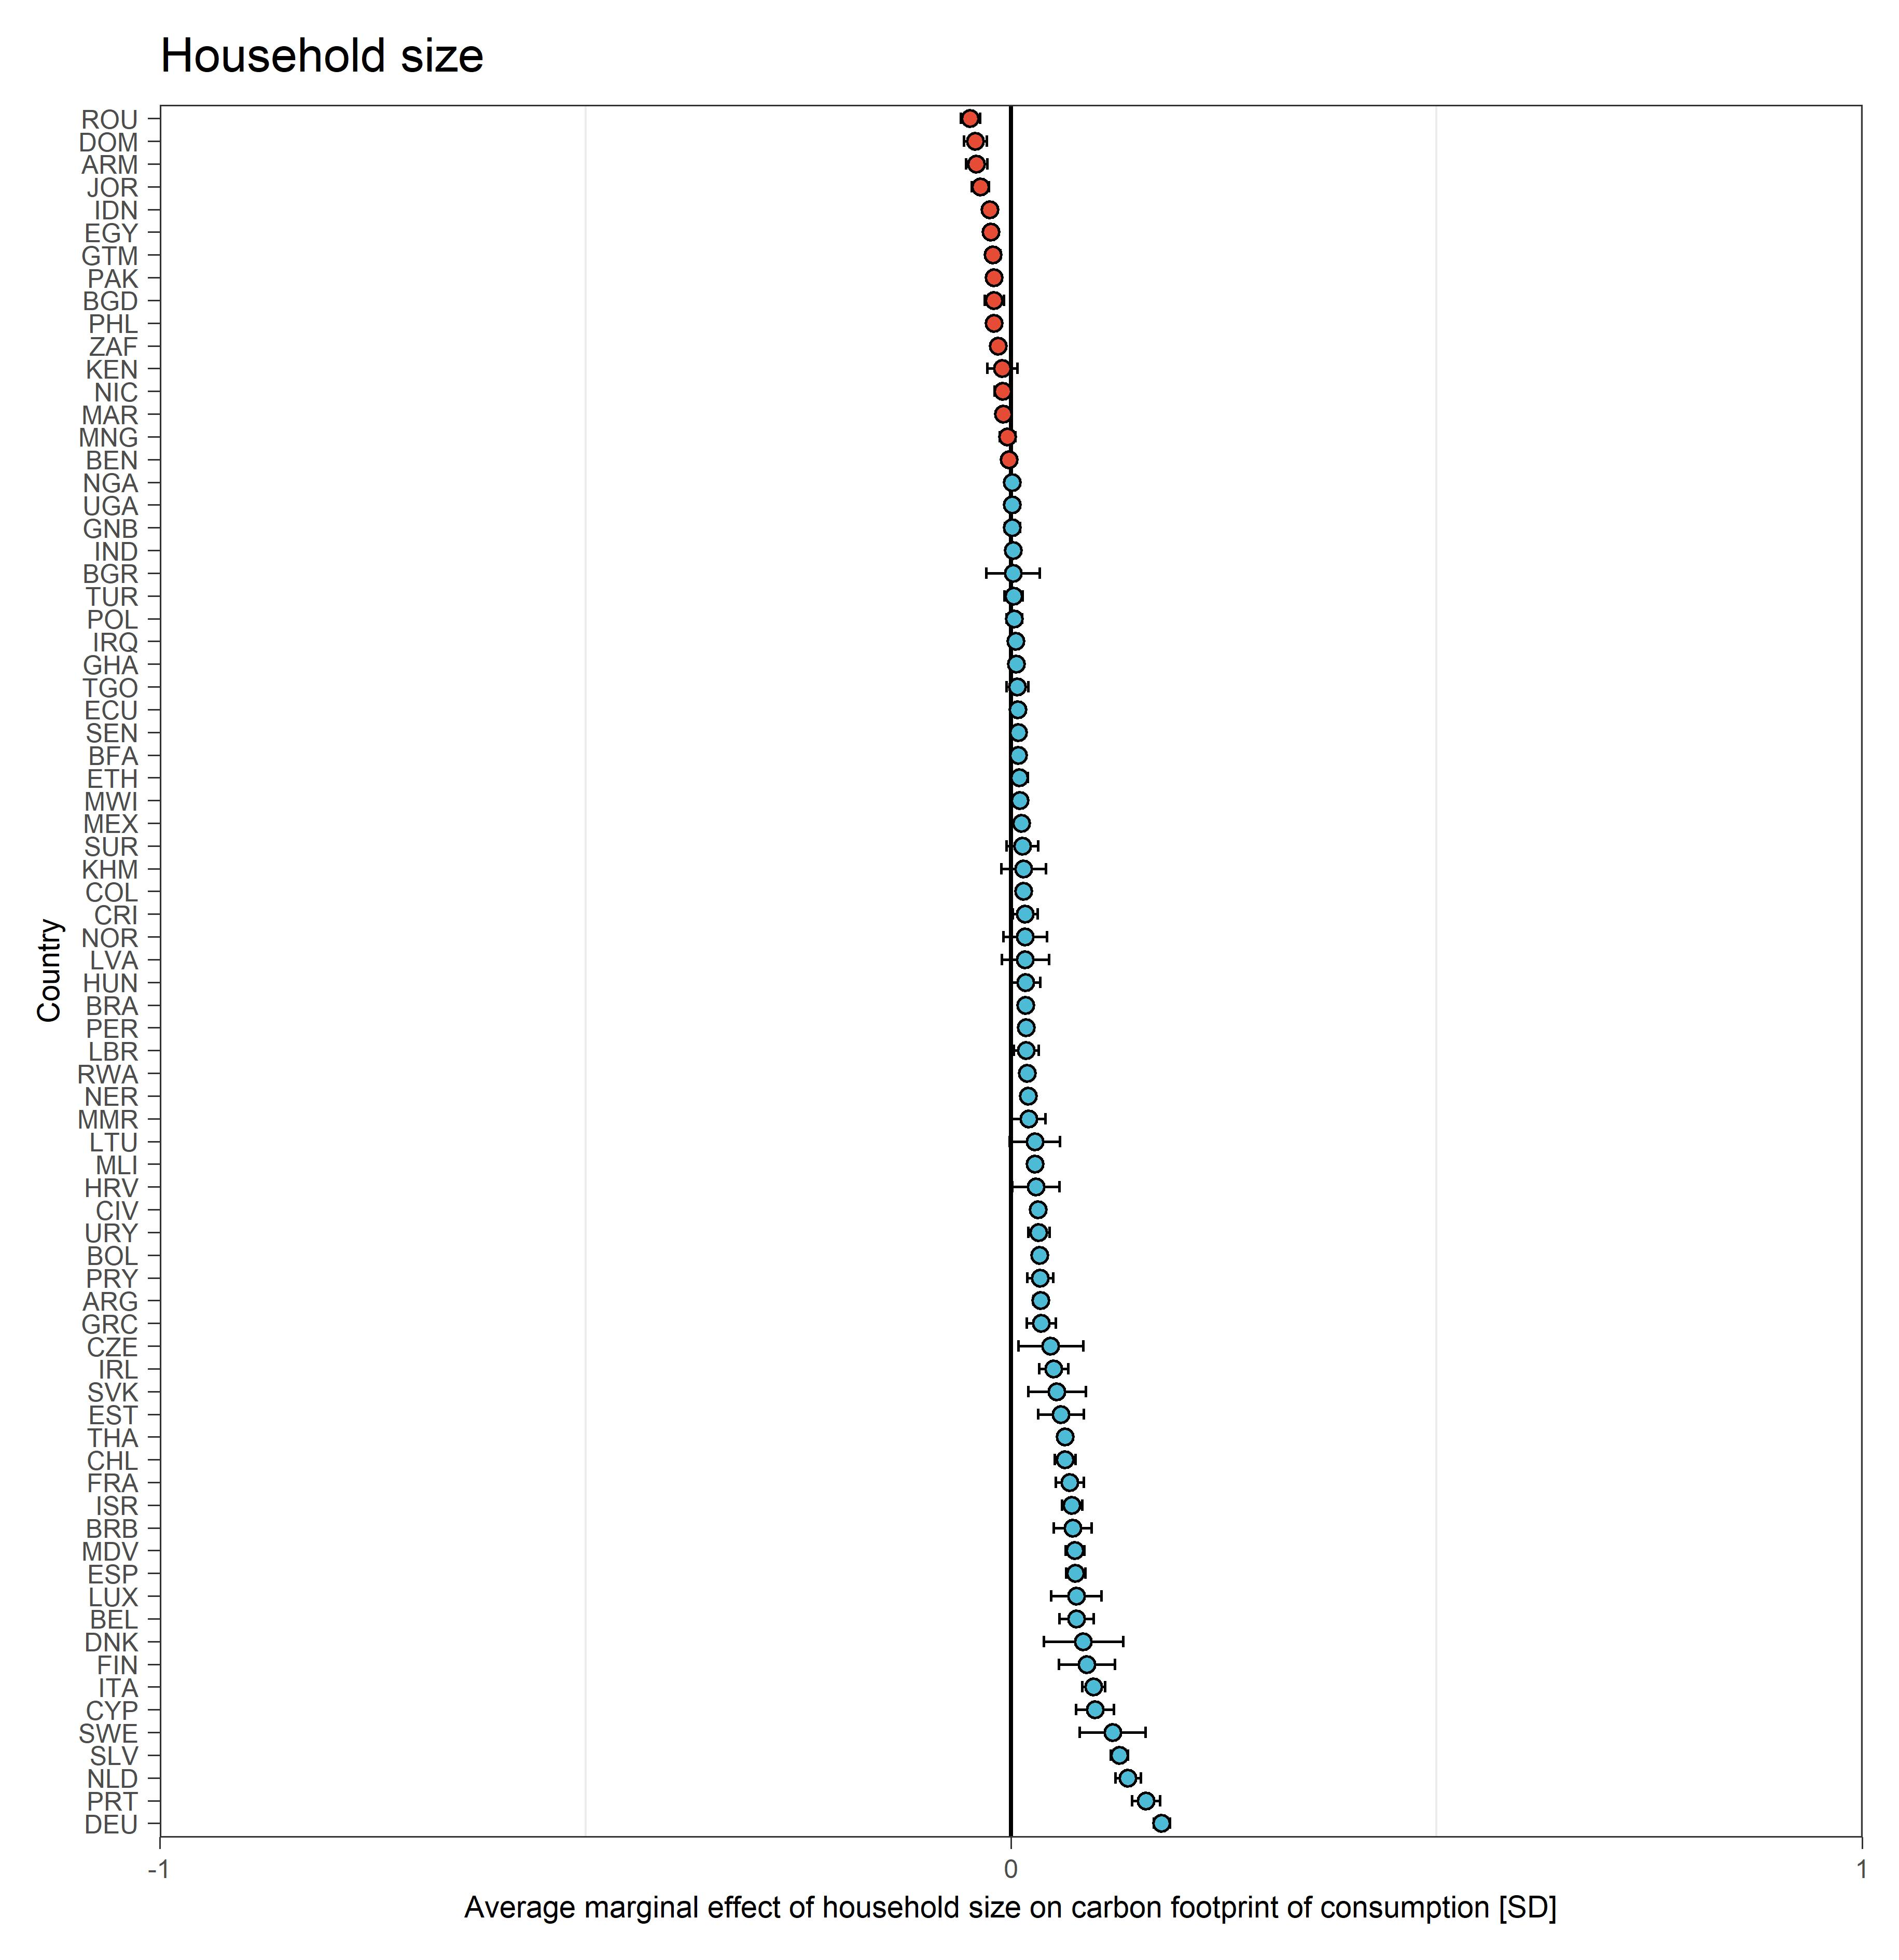
\includegraphics{Analysis_OLS_ME_Carbon_Footprint/AME_OLS_FP_hh_size}
%   \begin{subcaption}
%     This figure displays ...
%   \end{subcaption}

% \end{figure}

% \clearpage

% \begin{figure}[ht!]
%   \centering
%  \caption{Average marginal effects of household expenditures} \label{fig:D4_Expenditures}
%   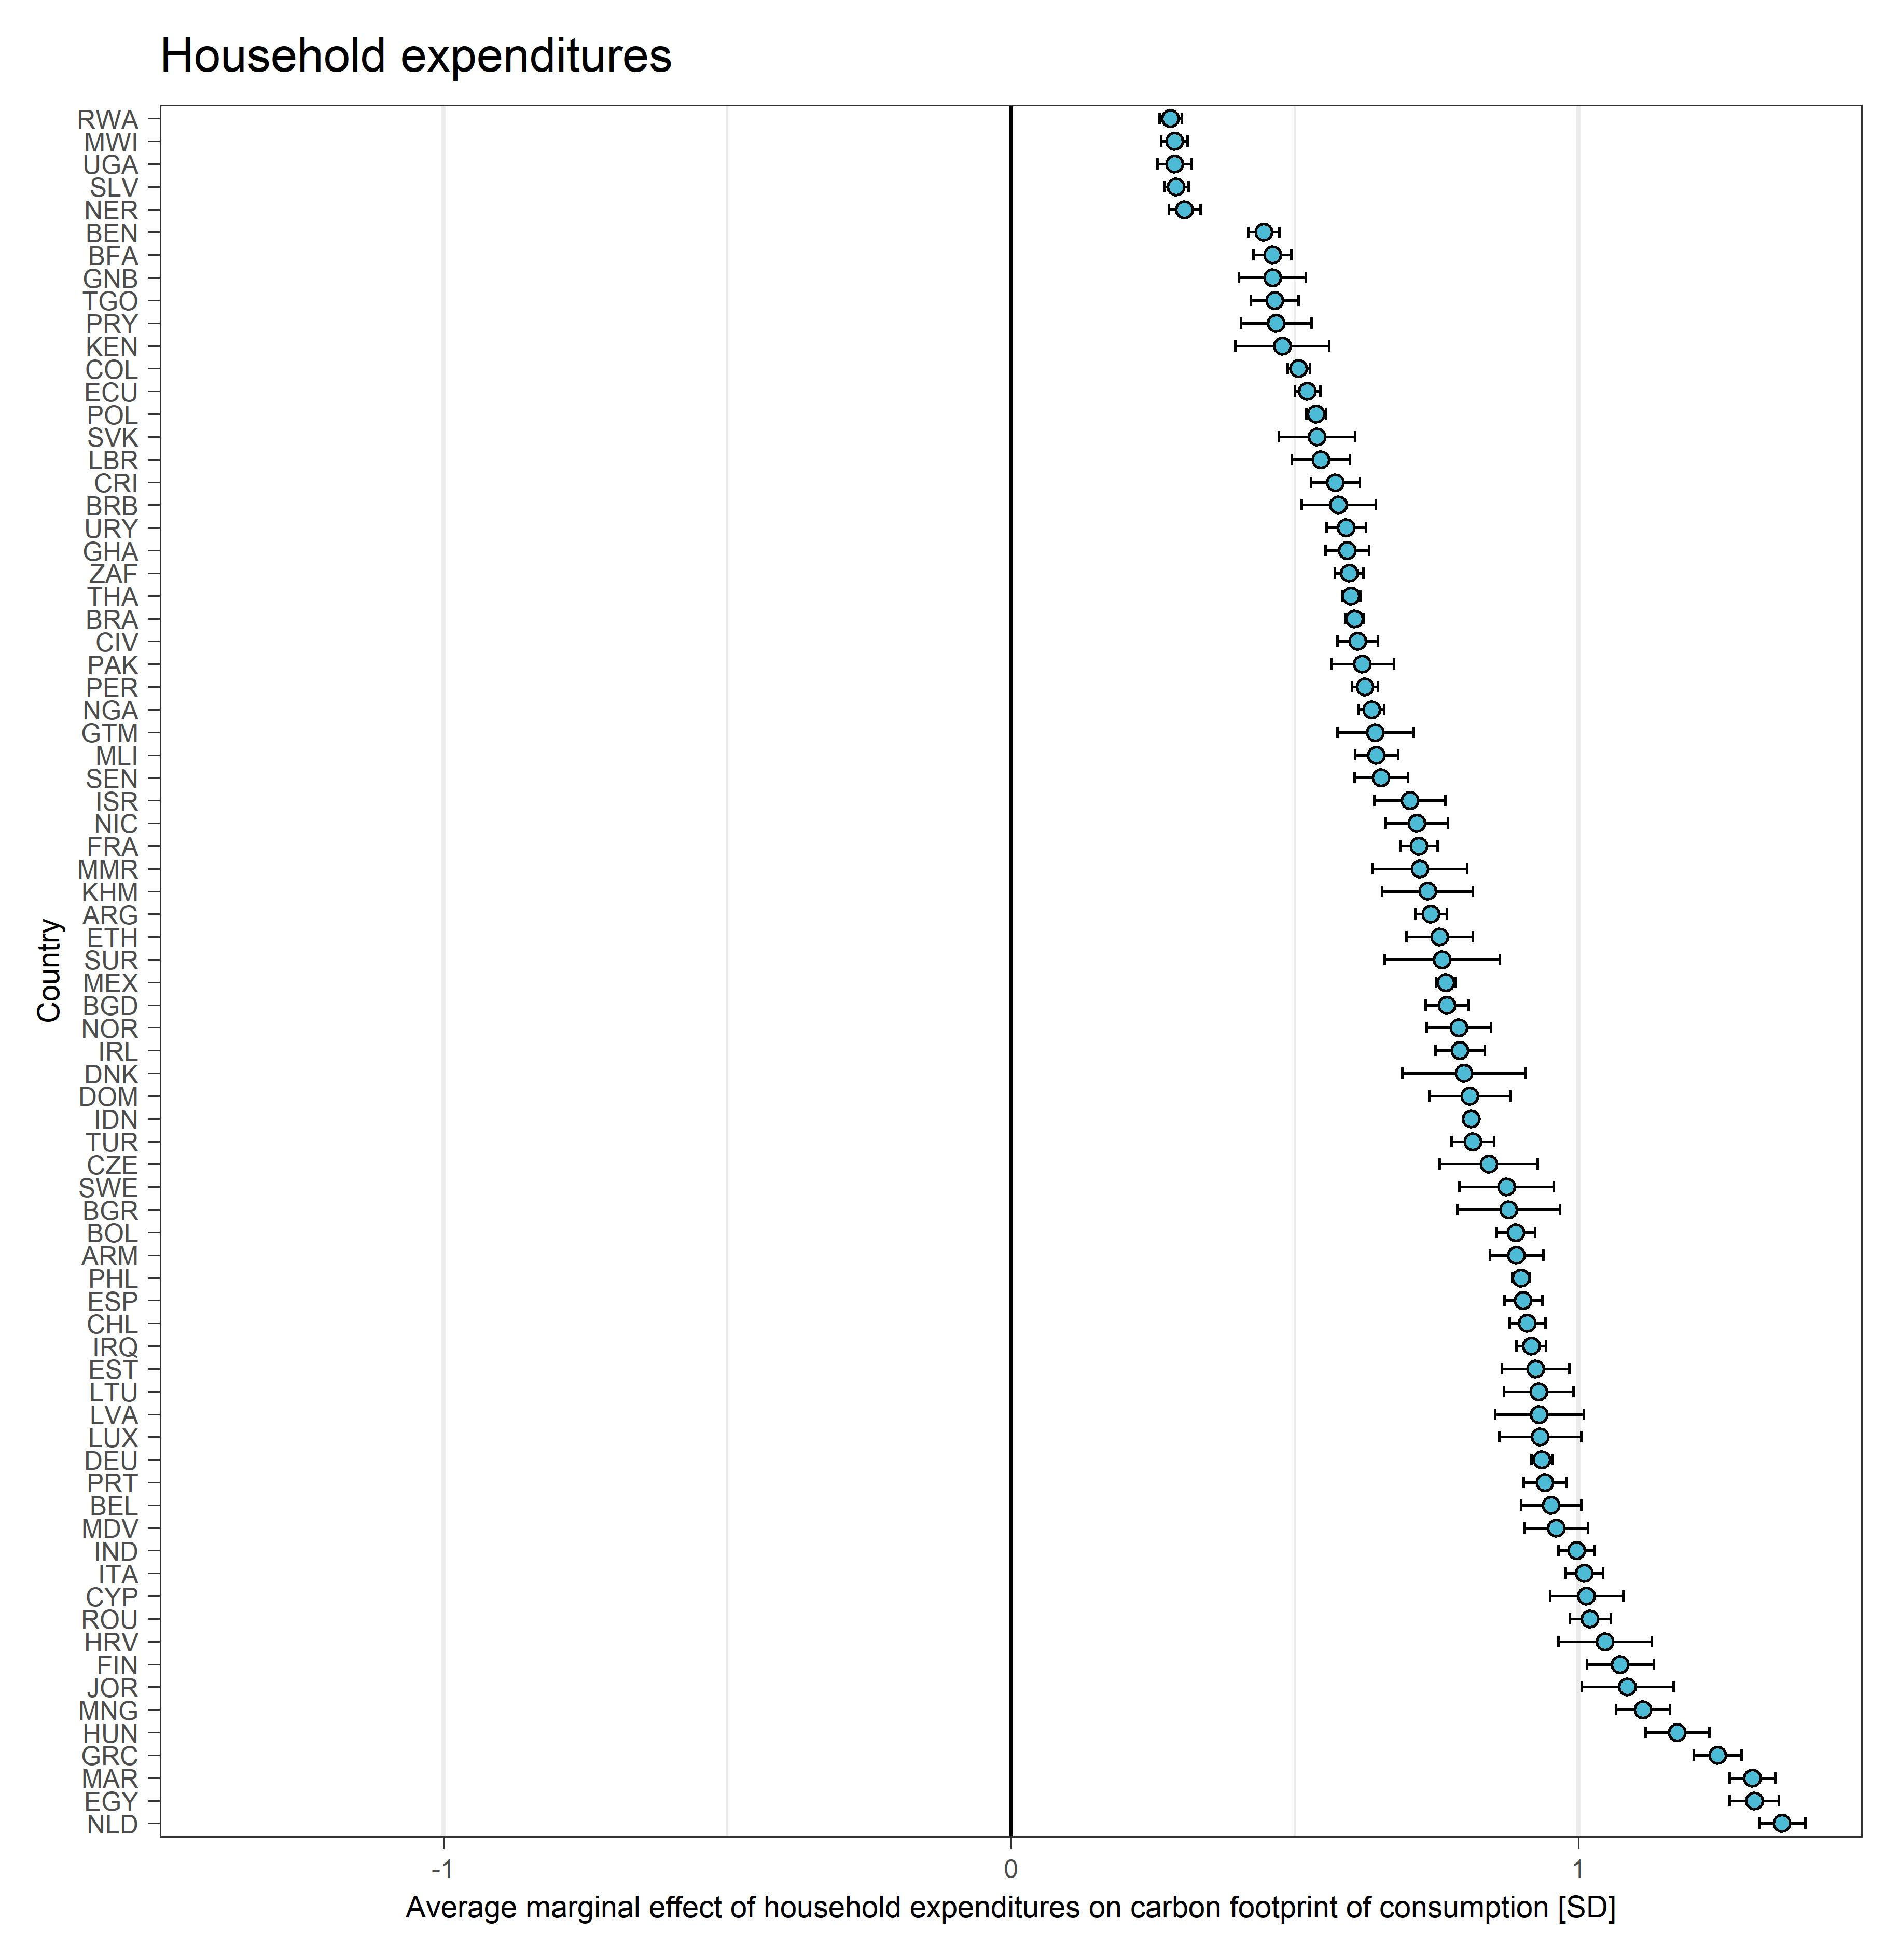
\includegraphics{Analysis_OLS_ME_Carbon_Footprint/AME_OLS_FP_log_hh_expenditures_USD_2014}
%   \begin{subcaption}
%     This figure displays ...
%   \end{subcaption}

% \end{figure}

% \clearpage

% \begin{figure}[ht!]
%   \centering
%  \caption{Average marginal effects of urban citizenship} \label{fig:D5_Urban}
%   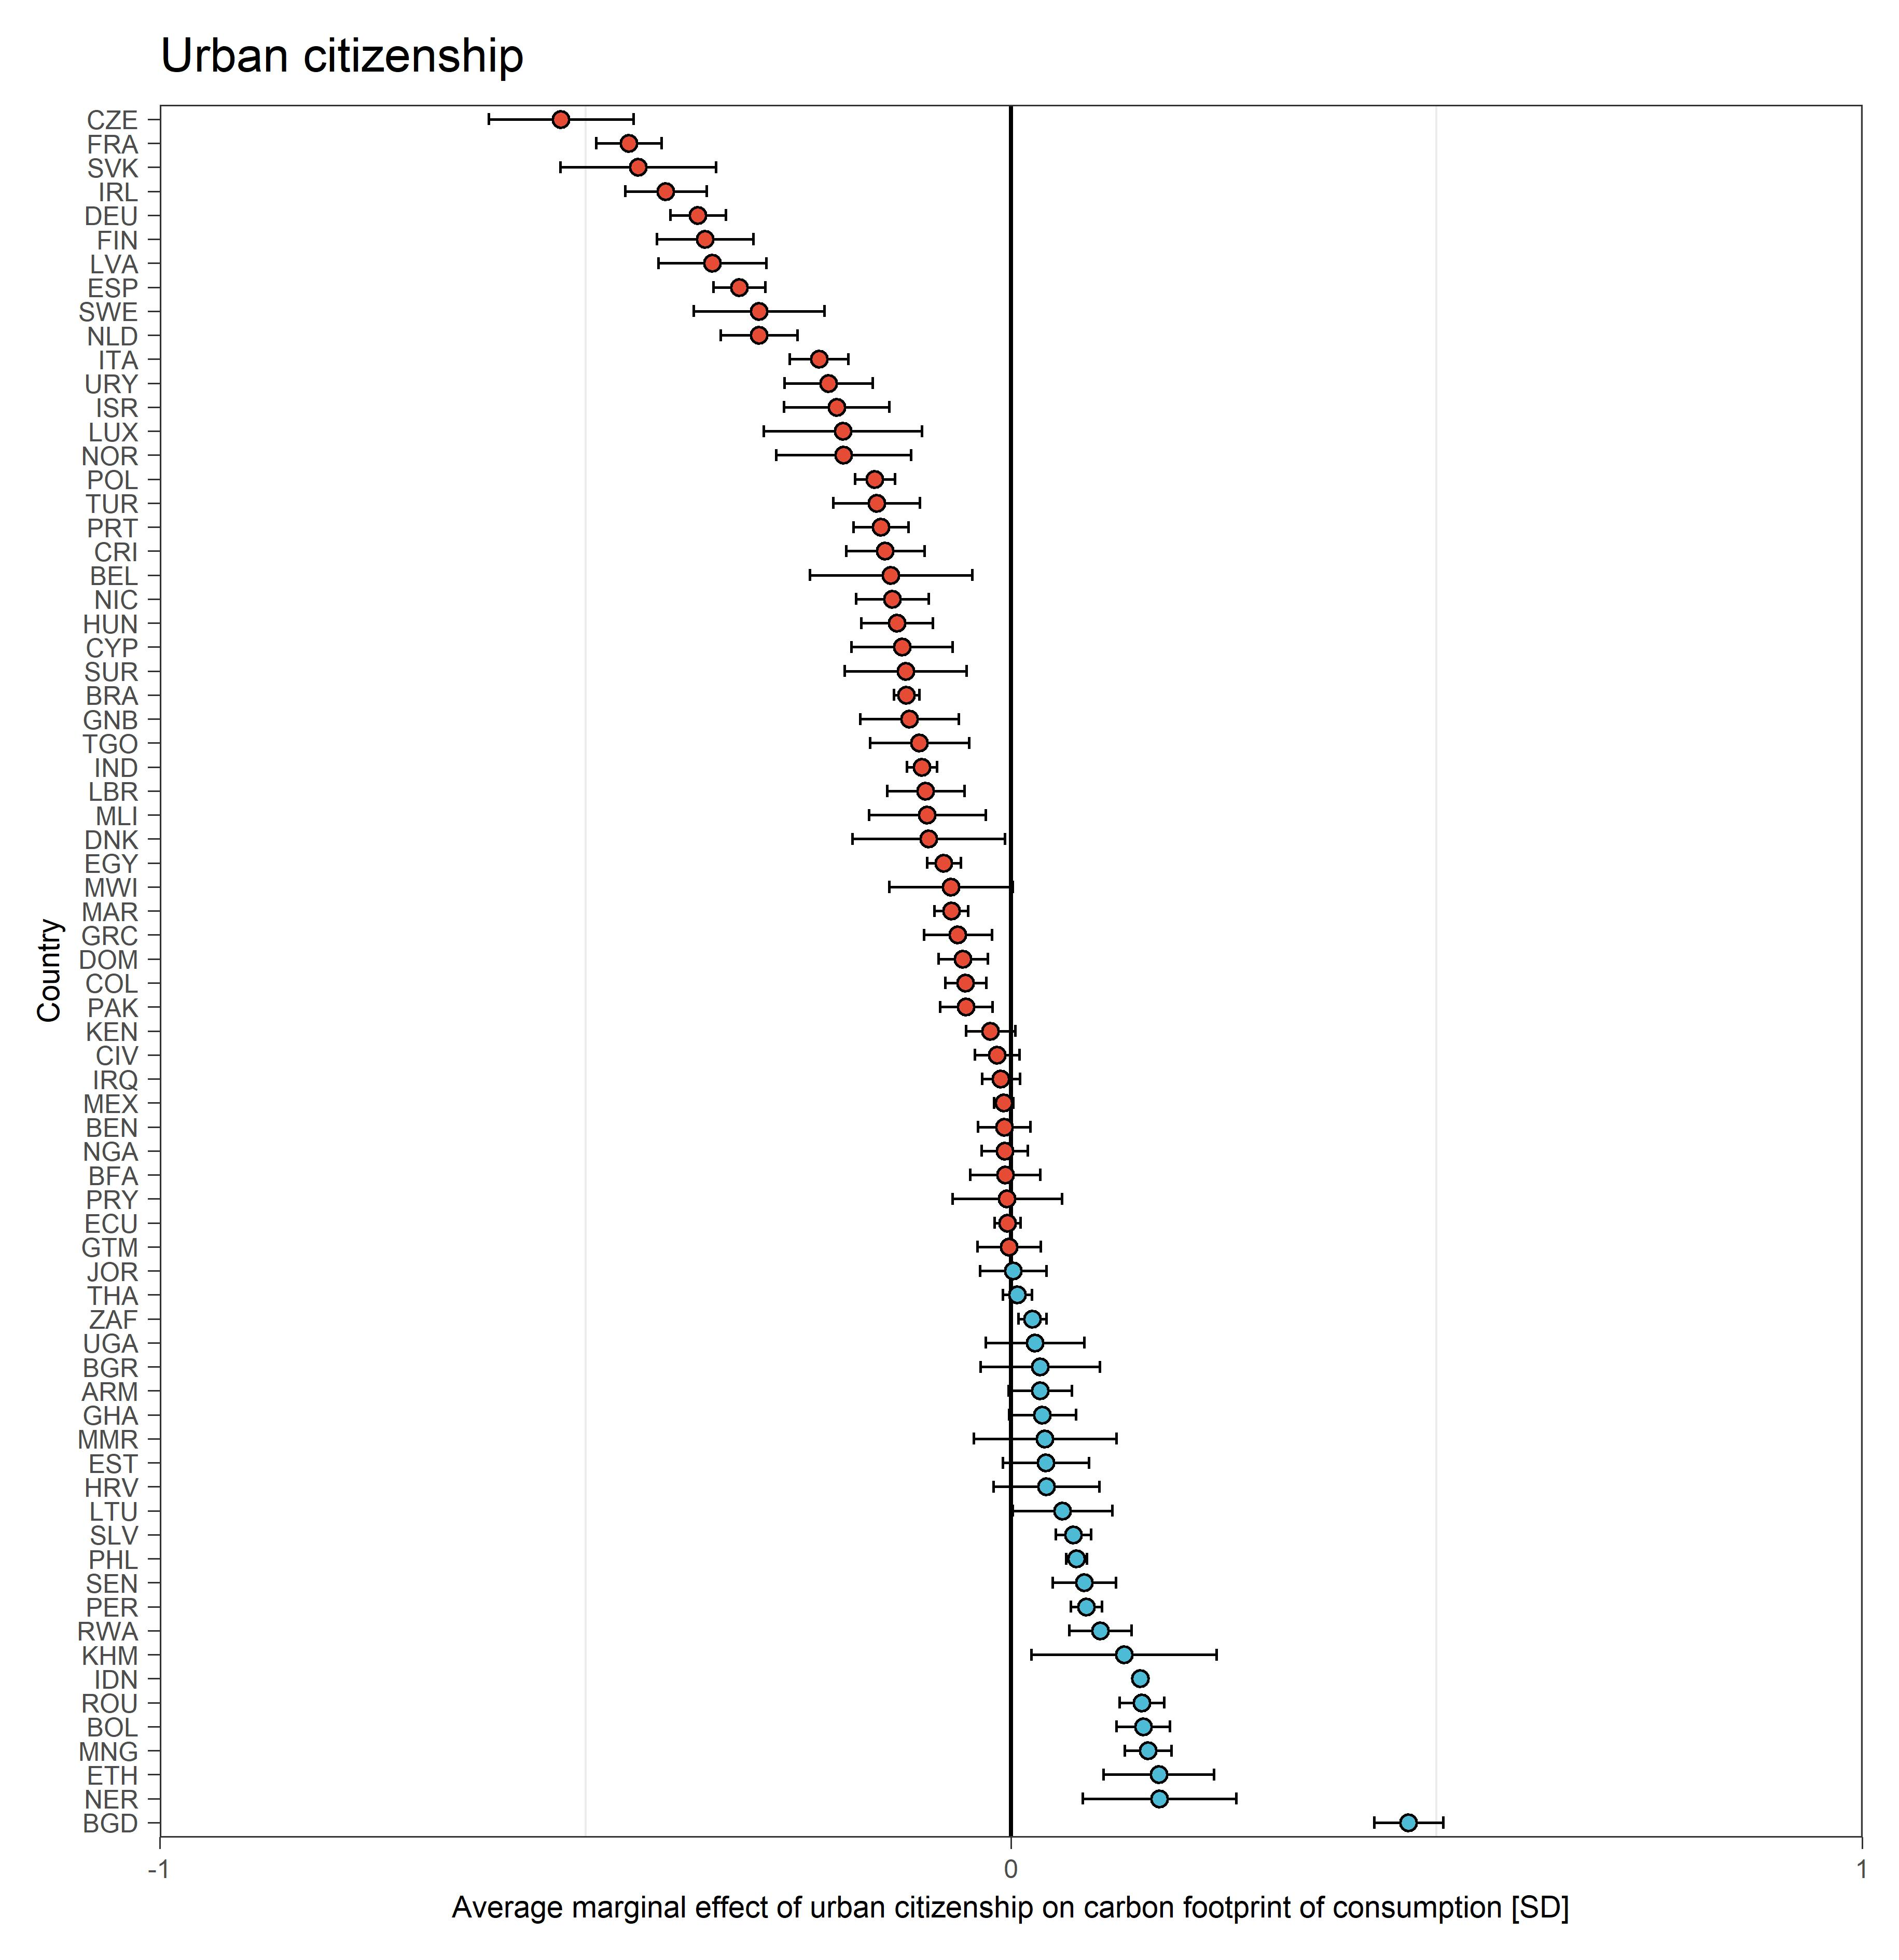
\includegraphics{Analysis_OLS_ME_Carbon_Footprint/AME_OLS_FP_urban_01}
%   \begin{subcaption}
%     This figure displays ...
%   \end{subcaption}

% \end{figure}

% \clearpage

% \begin{figure}[ht!]
%   \centering
%  \caption{Average marginal effects of cooking fuel choice - Part A} \label{fig:D6_Electricity_A}
%   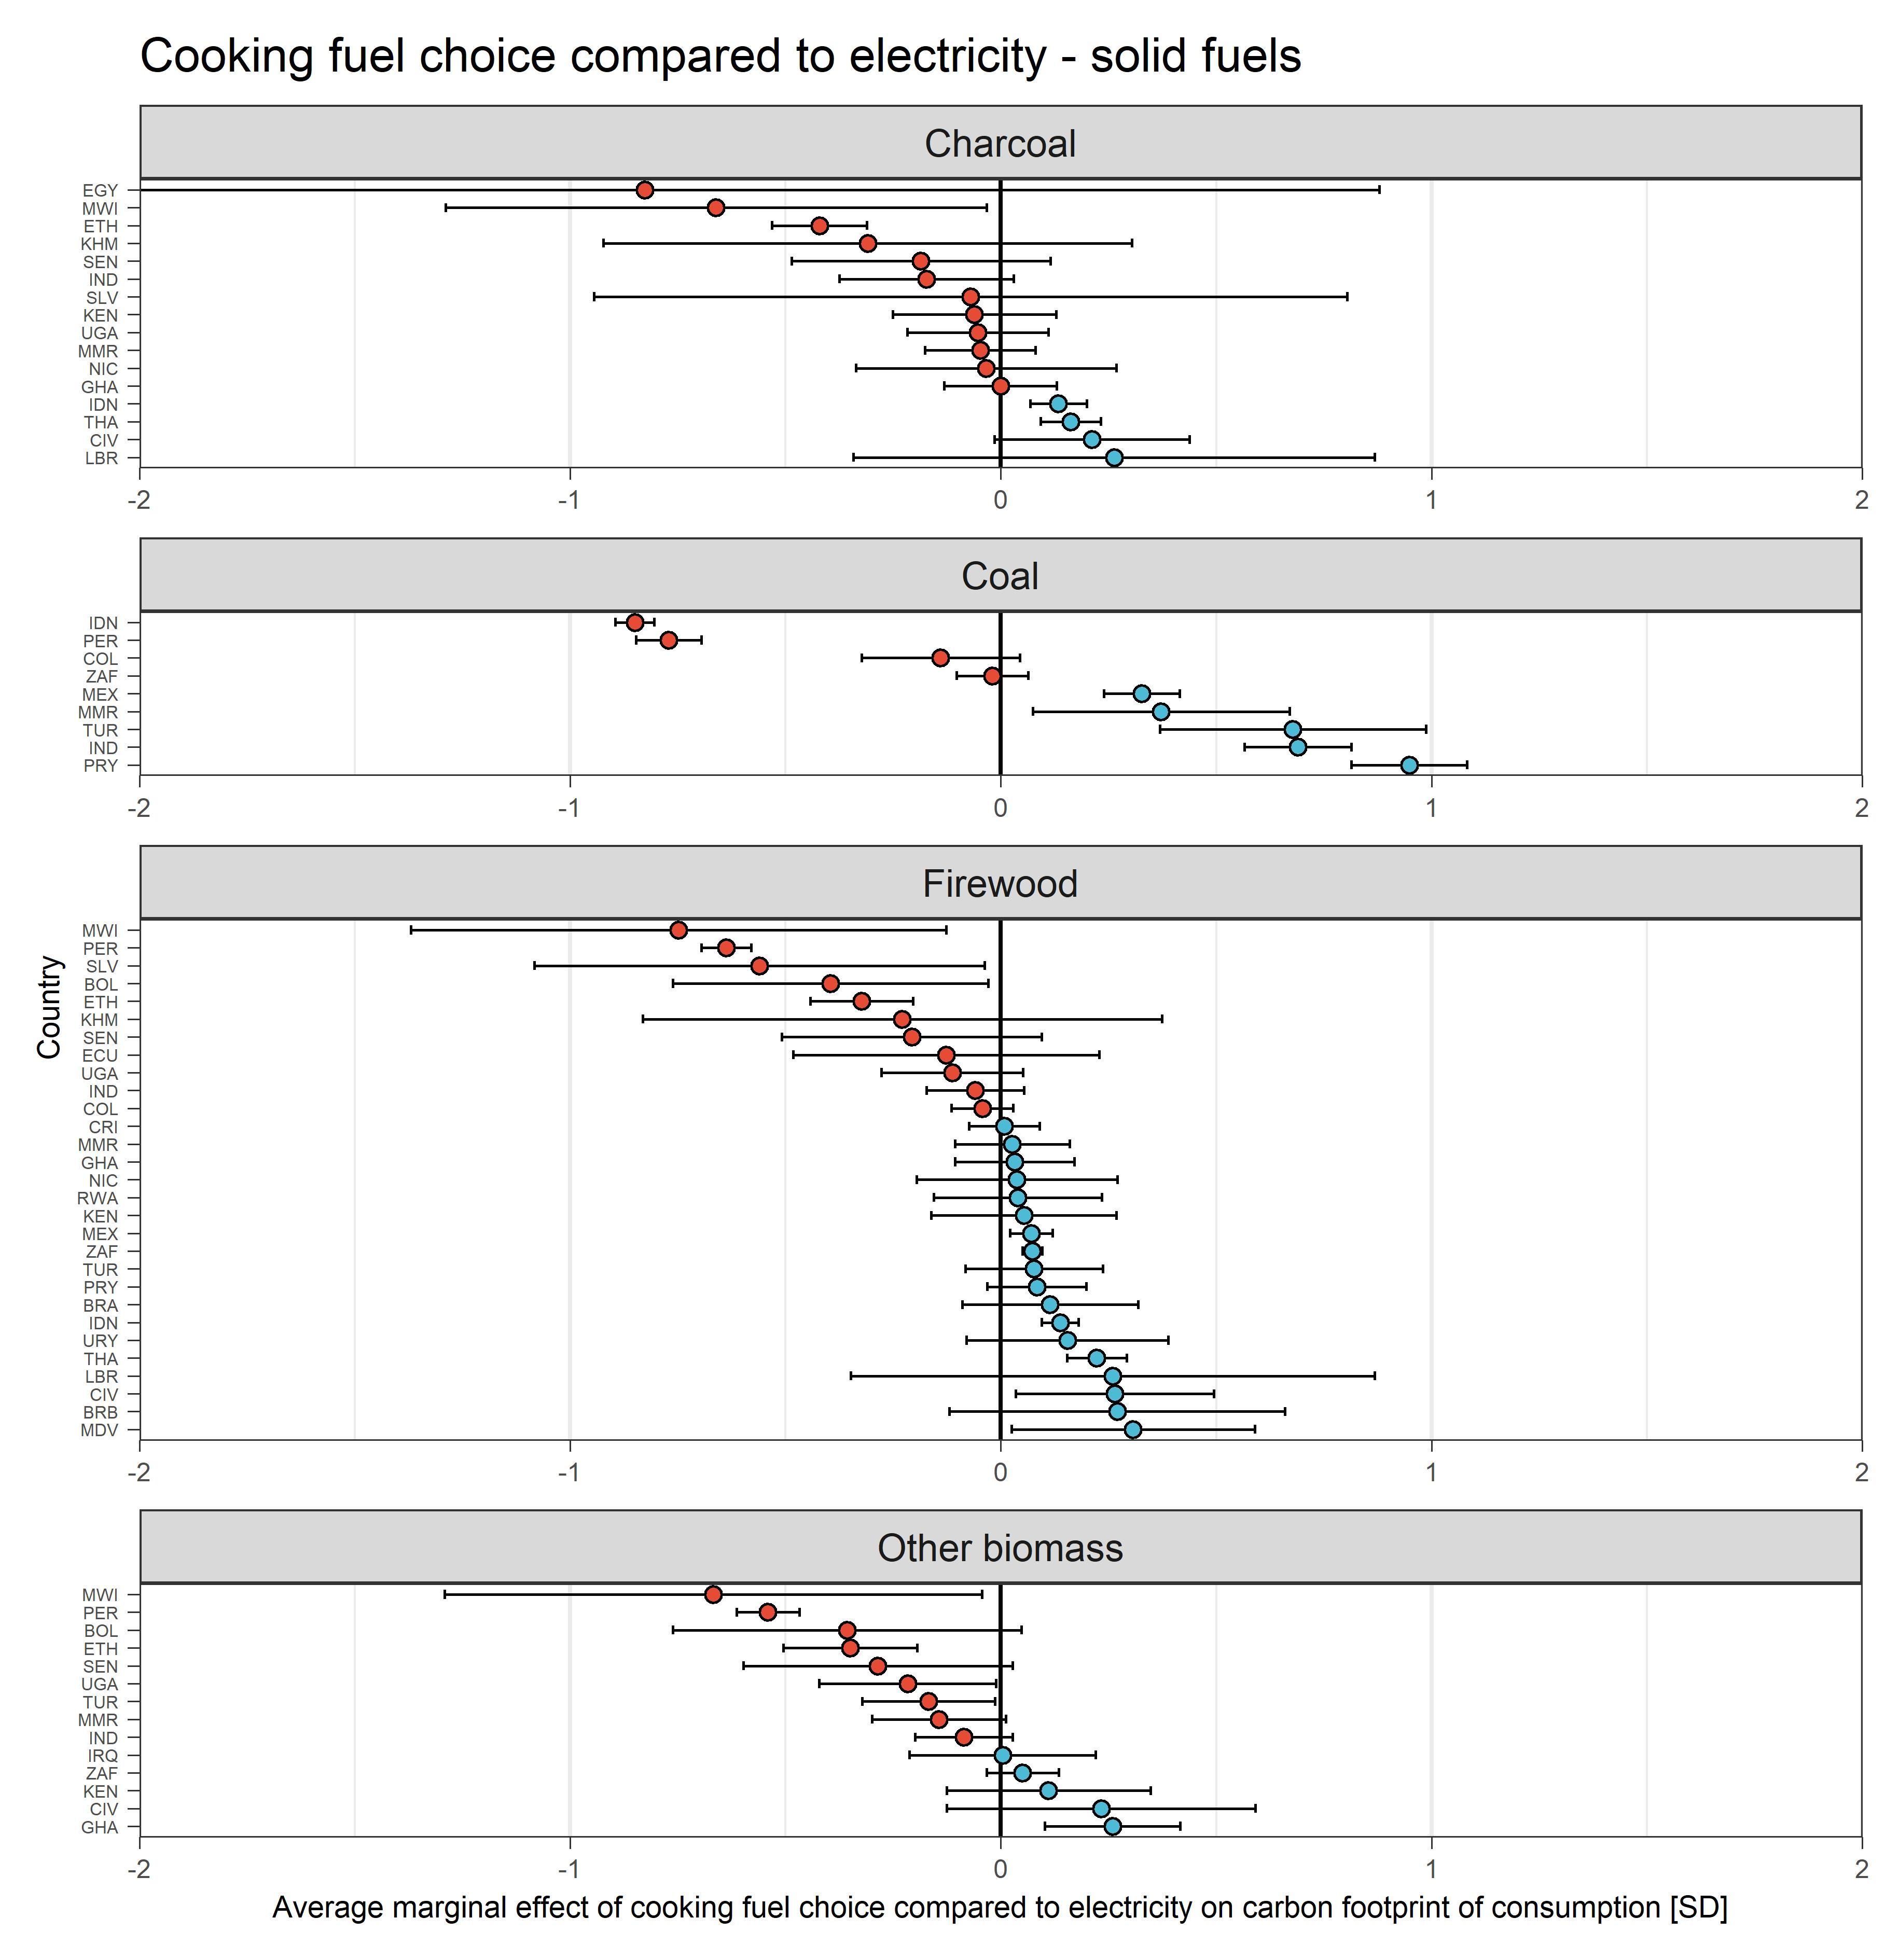
\includegraphics{Analysis_OLS_ME_Carbon_Footprint/AME_OLS_FP_CF_Electricity A}
%   \begin{subcaption}
%     This figure displays ...
%   \end{subcaption}

% \end{figure}

% \clearpage

% \begin{figure}[ht!]
%   \centering
%  \caption{Average marginal effects of cooking fuel choice - Part B} \label{fig:D7_Electricity_B}
%   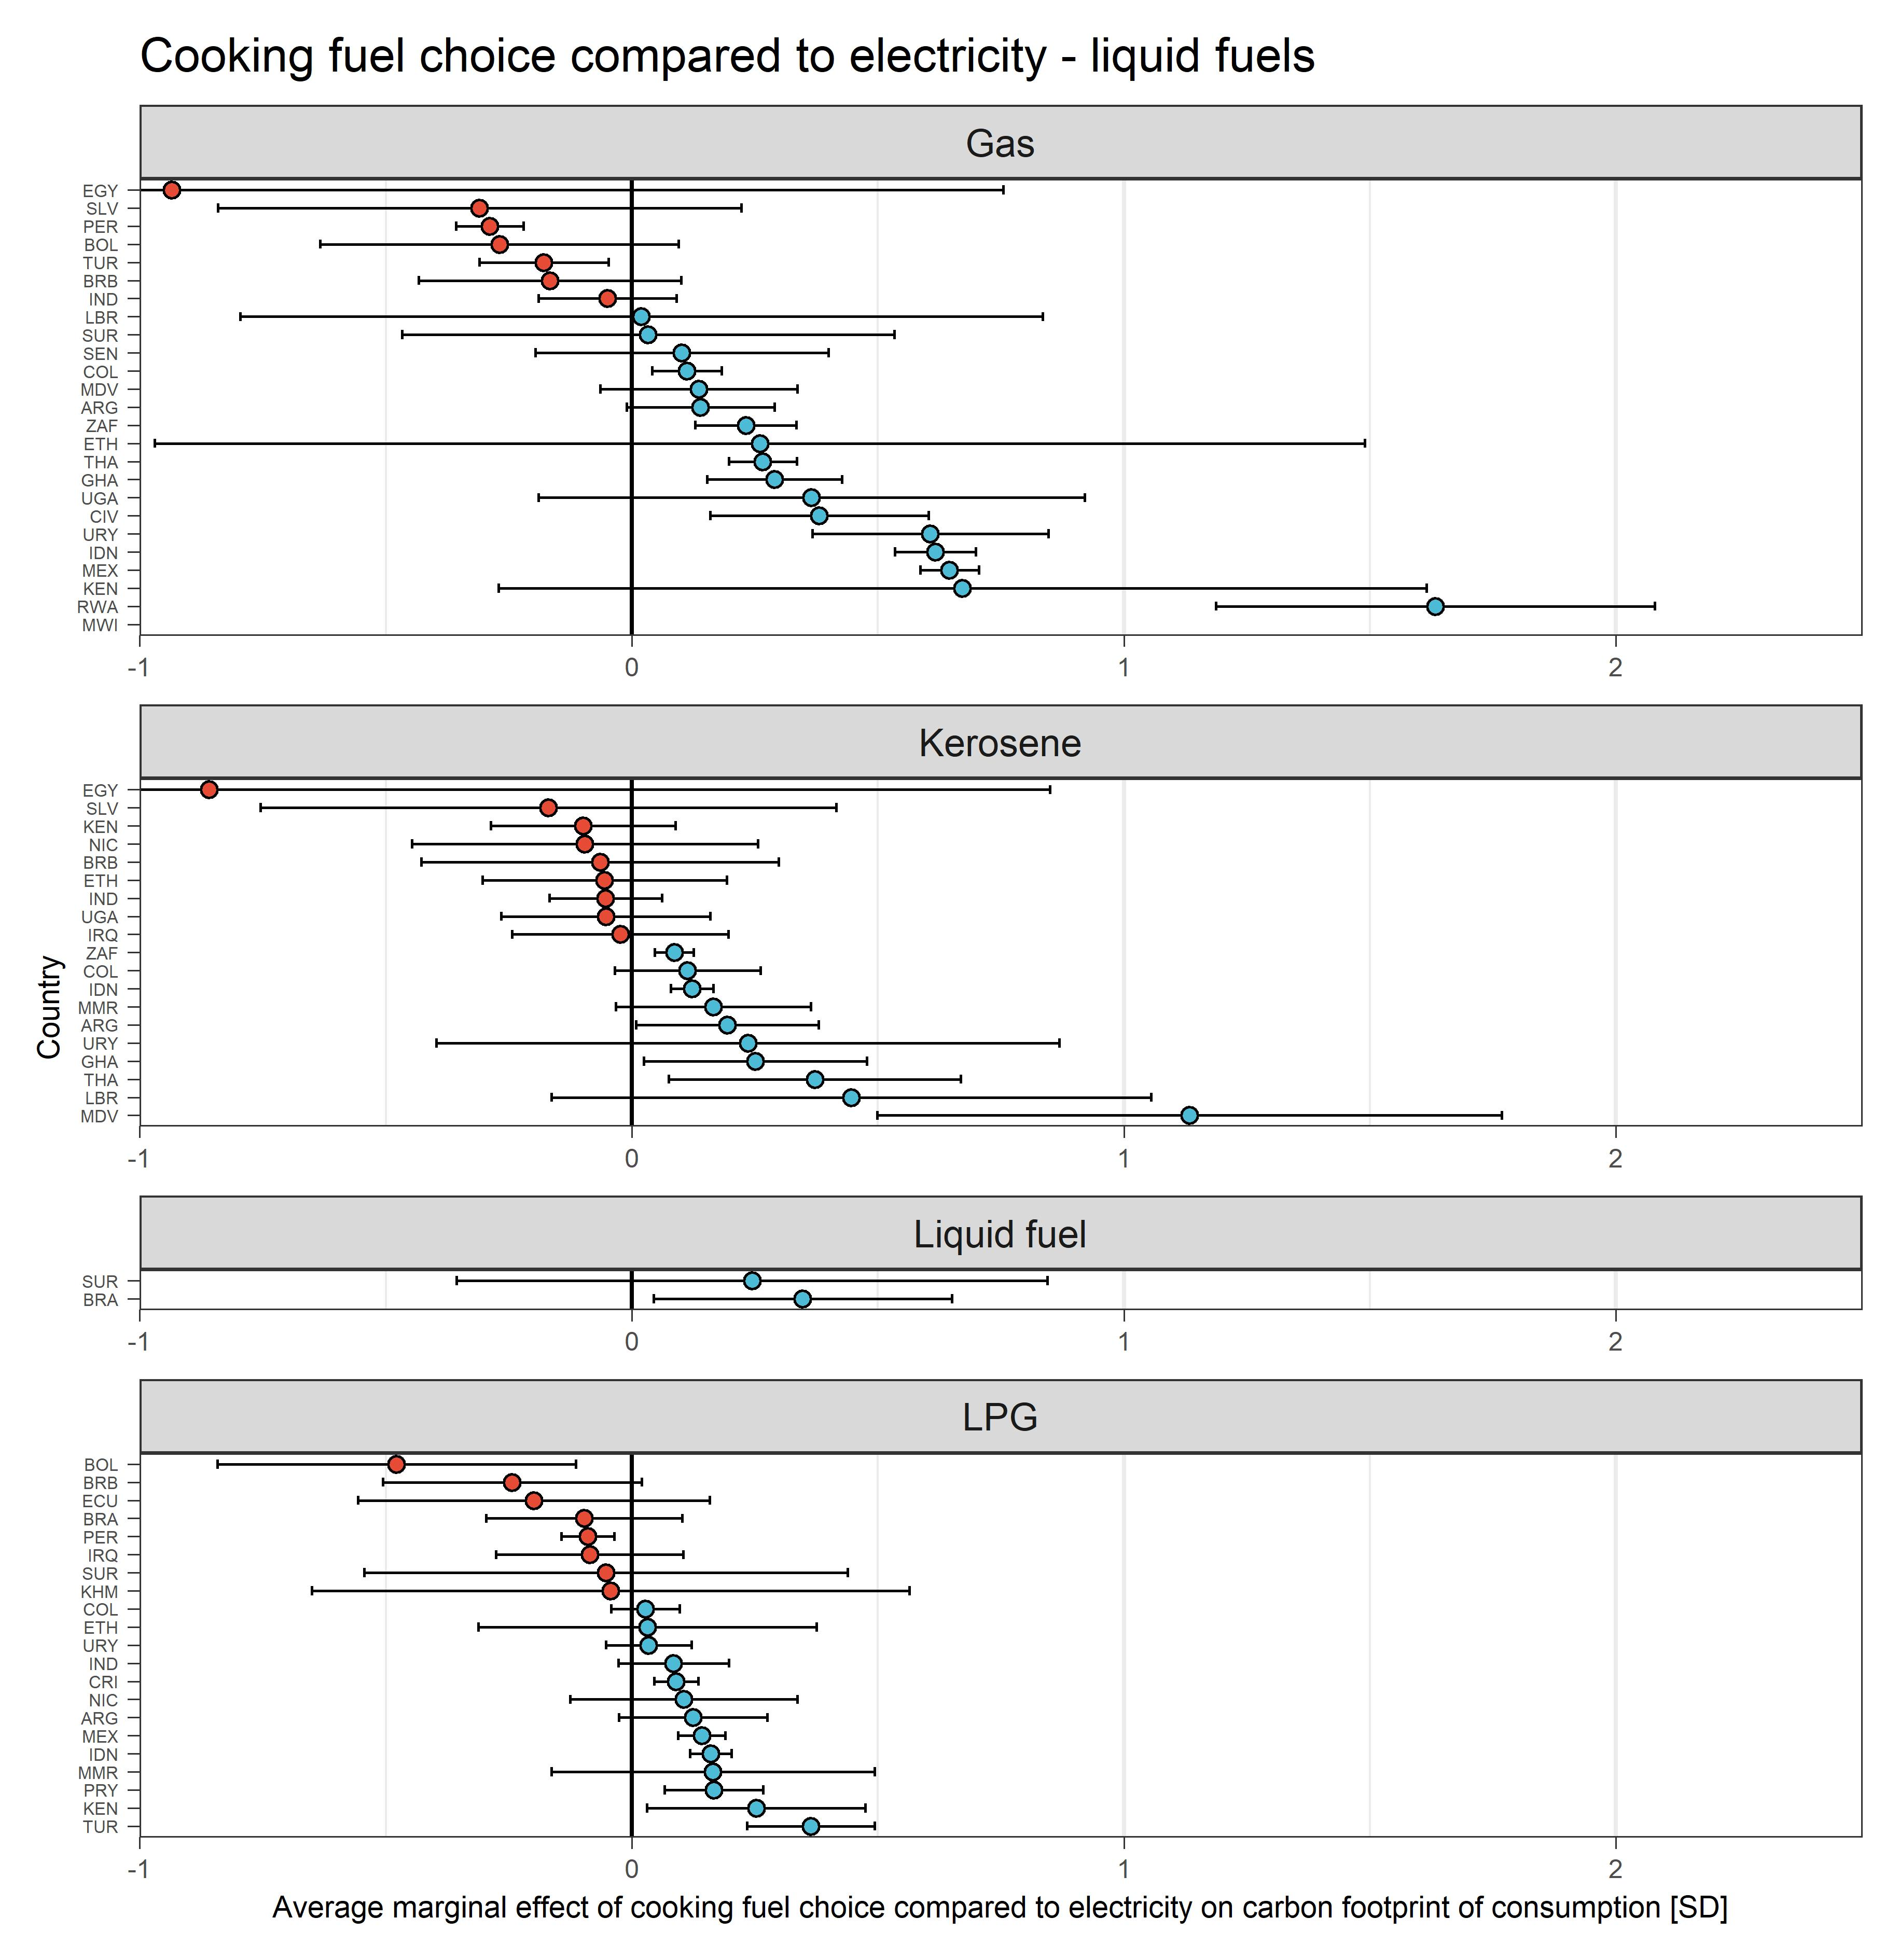
\includegraphics{Analysis_OLS_ME_Carbon_Footprint/AME_OLS_FP_CF_Electricity B}
%   \begin{subcaption}
%     This figure displays ...
%   \end{subcaption}

% \end{figure}

% \clearpage

% \begin{figure}[ht!]
%   \centering
%  \caption{Average marginal effects of cooking fuel choice - Part C} \label{fig:D8_LPG}
%   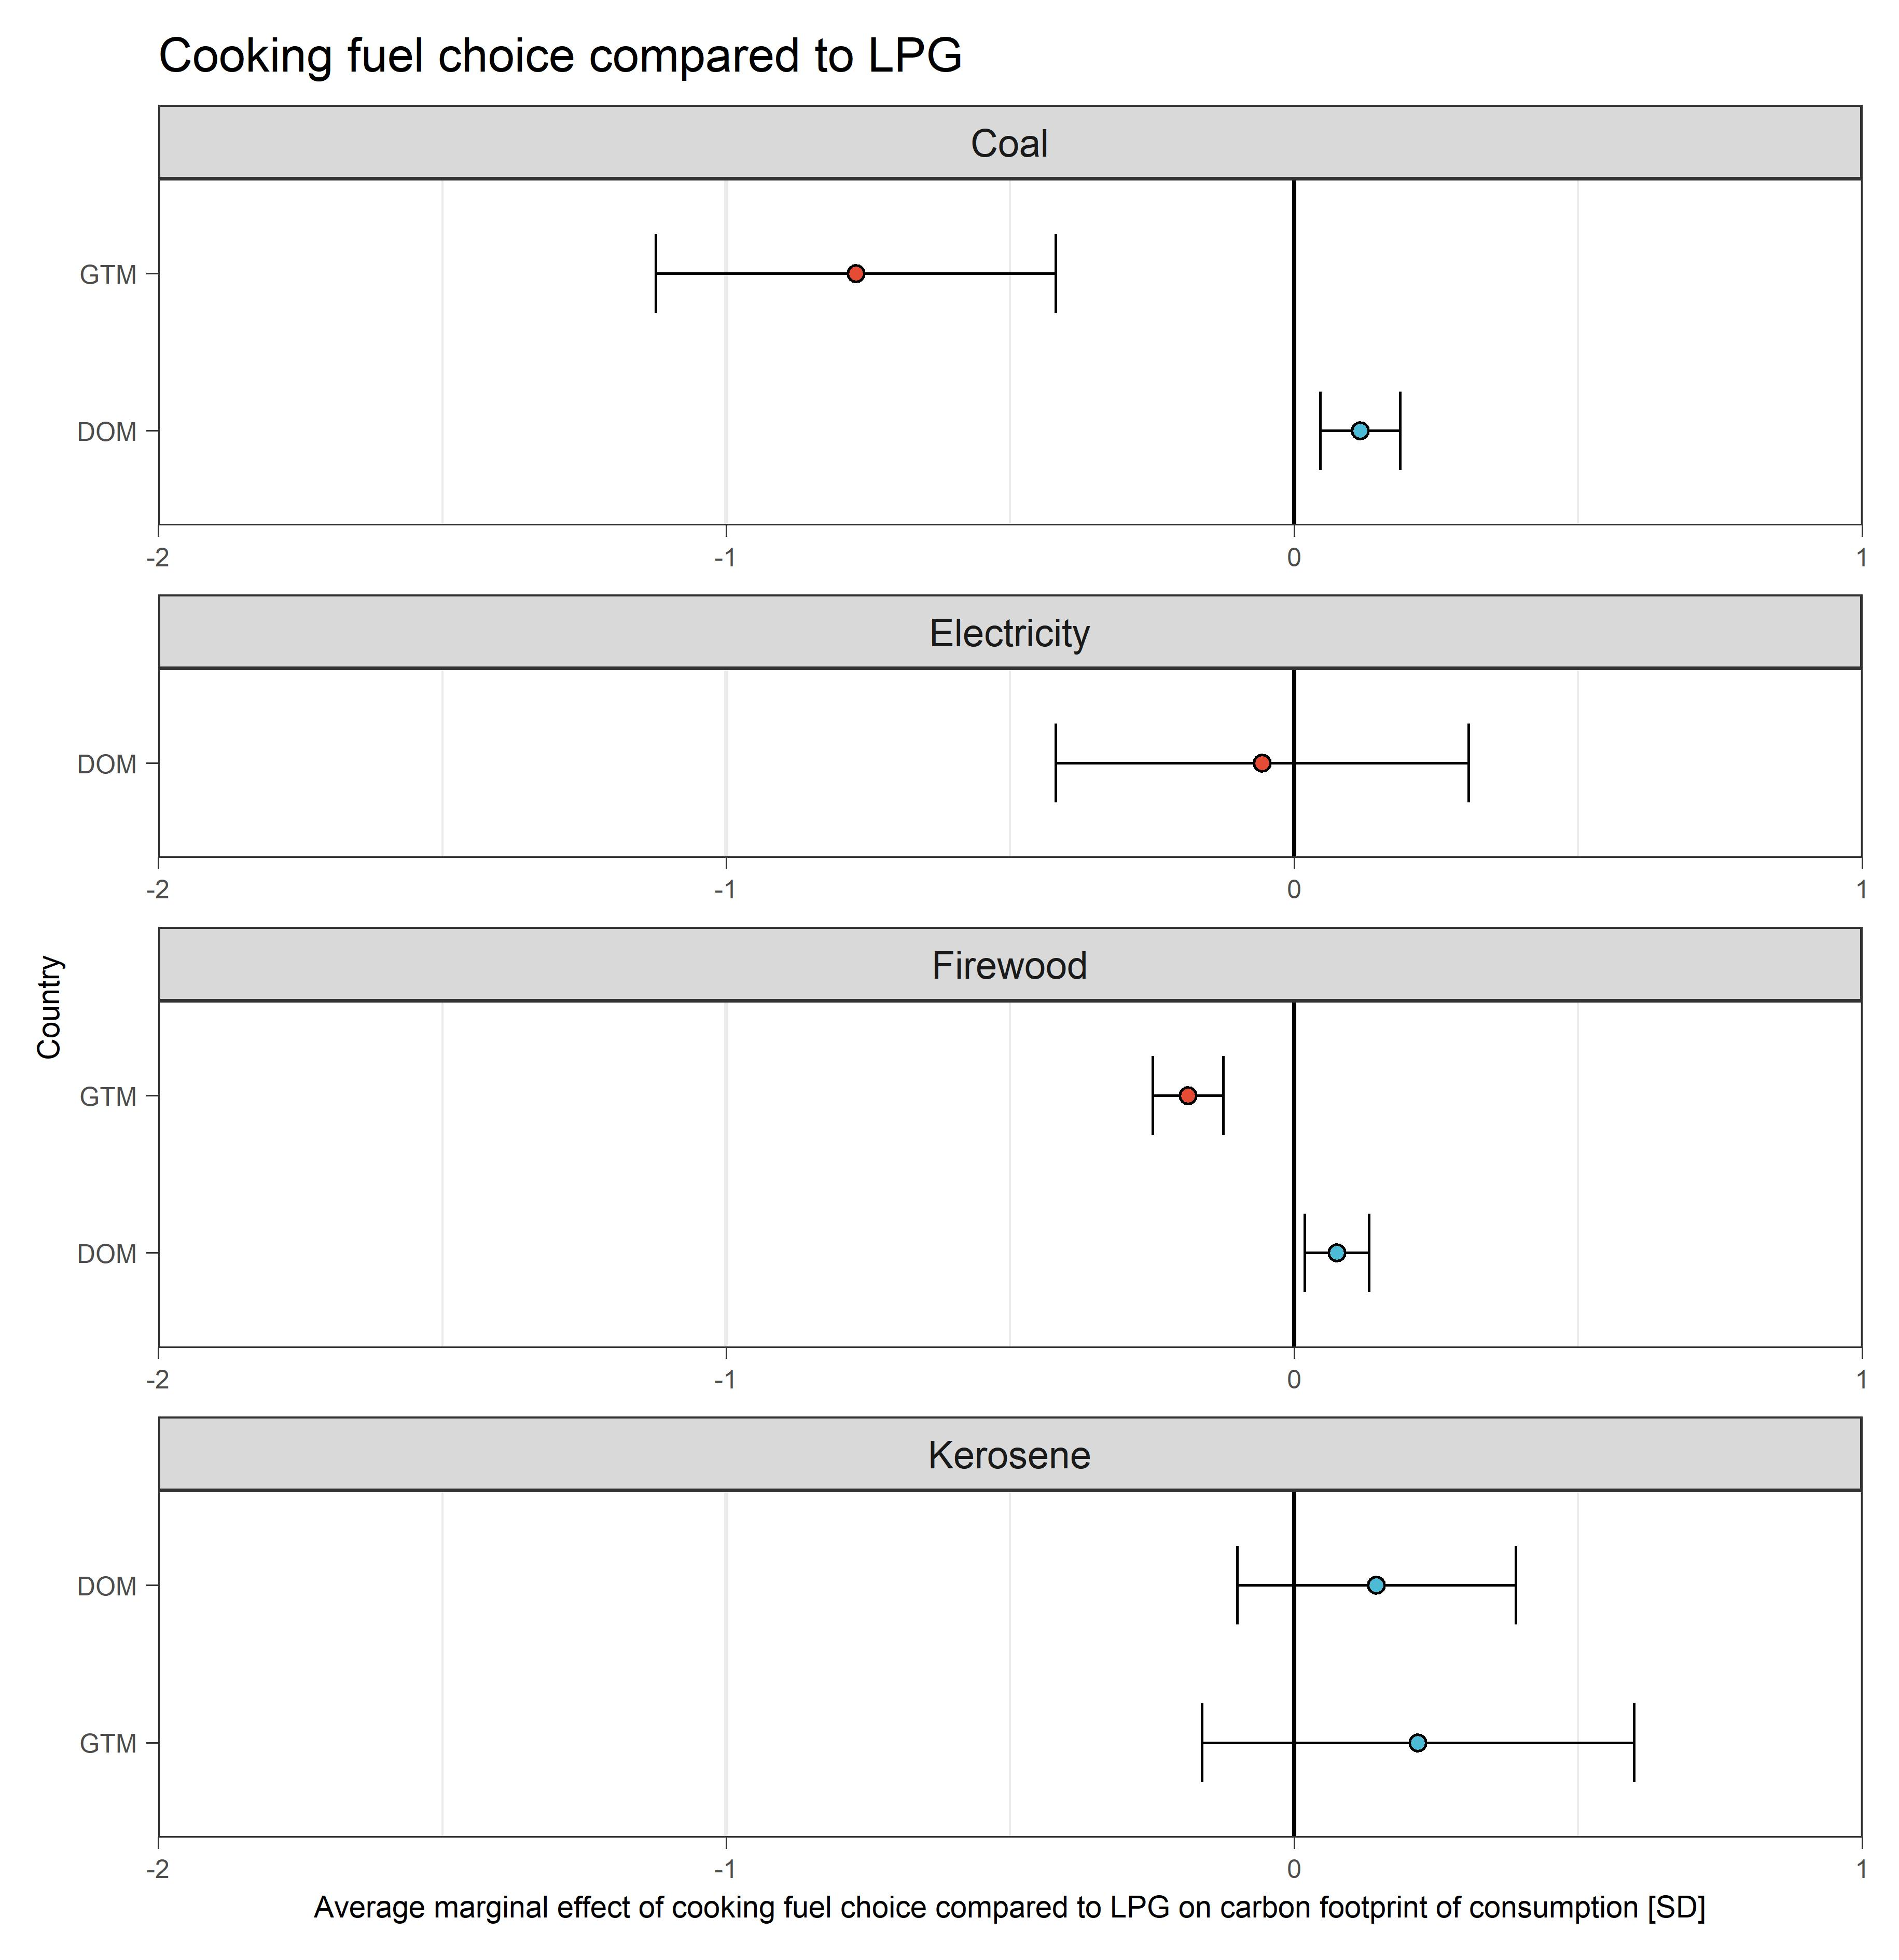
\includegraphics{Analysis_OLS_ME_Carbon_Footprint/AME_OLS_FP_CF_LPG}
%   \begin{subcaption}
%     This figure displays ...
%   \end{subcaption}

% \end{figure}

% \clearpage

% \begin{figure}[ht!]
%   \centering
%  \caption{Average marginal effects of cooking fuel choice - Part D} \label{fig:D9_Charcoal}
%   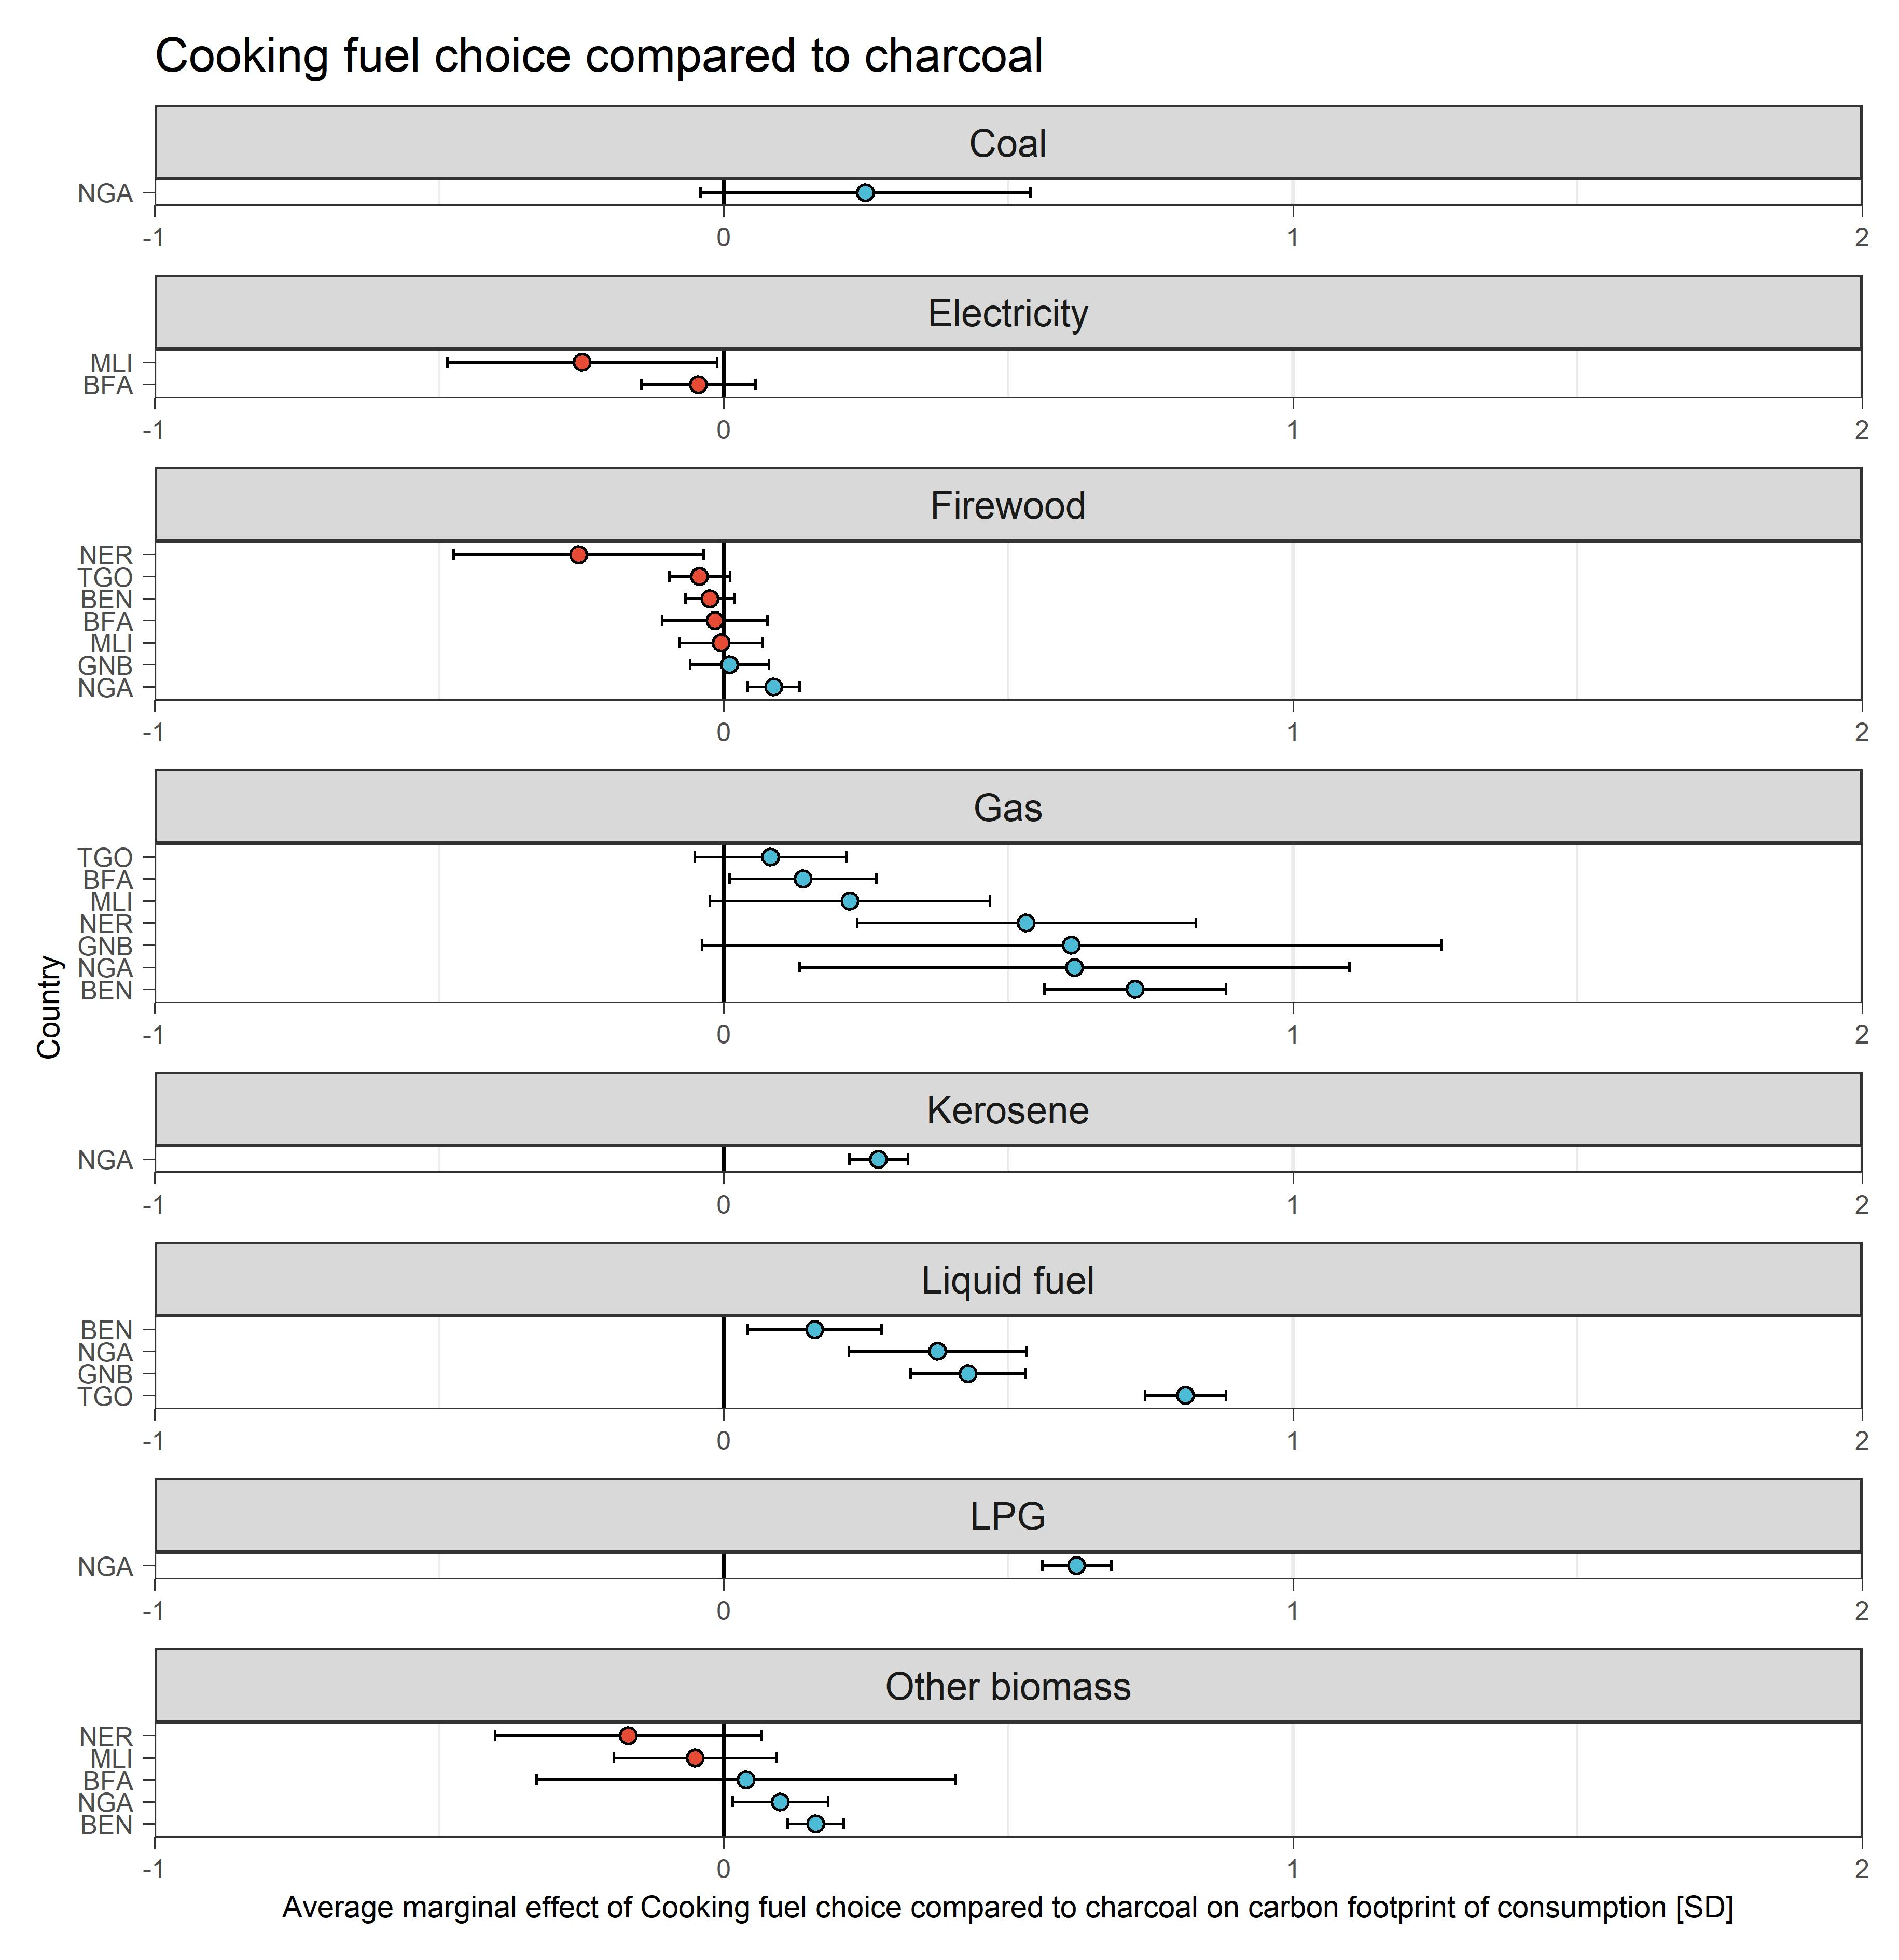
\includegraphics{Analysis_OLS_ME_Carbon_Footprint/AME_OLS_FP_CF_Charcoal}
%   \begin{subcaption}
%     This figure displays ...
%   \end{subcaption}

% \end{figure}

% \clearpage

% \begin{figure}[ht!]
%   \centering
%  \caption{Average marginal effects of secondary education} \label{fig:D10_sec_edu}
%   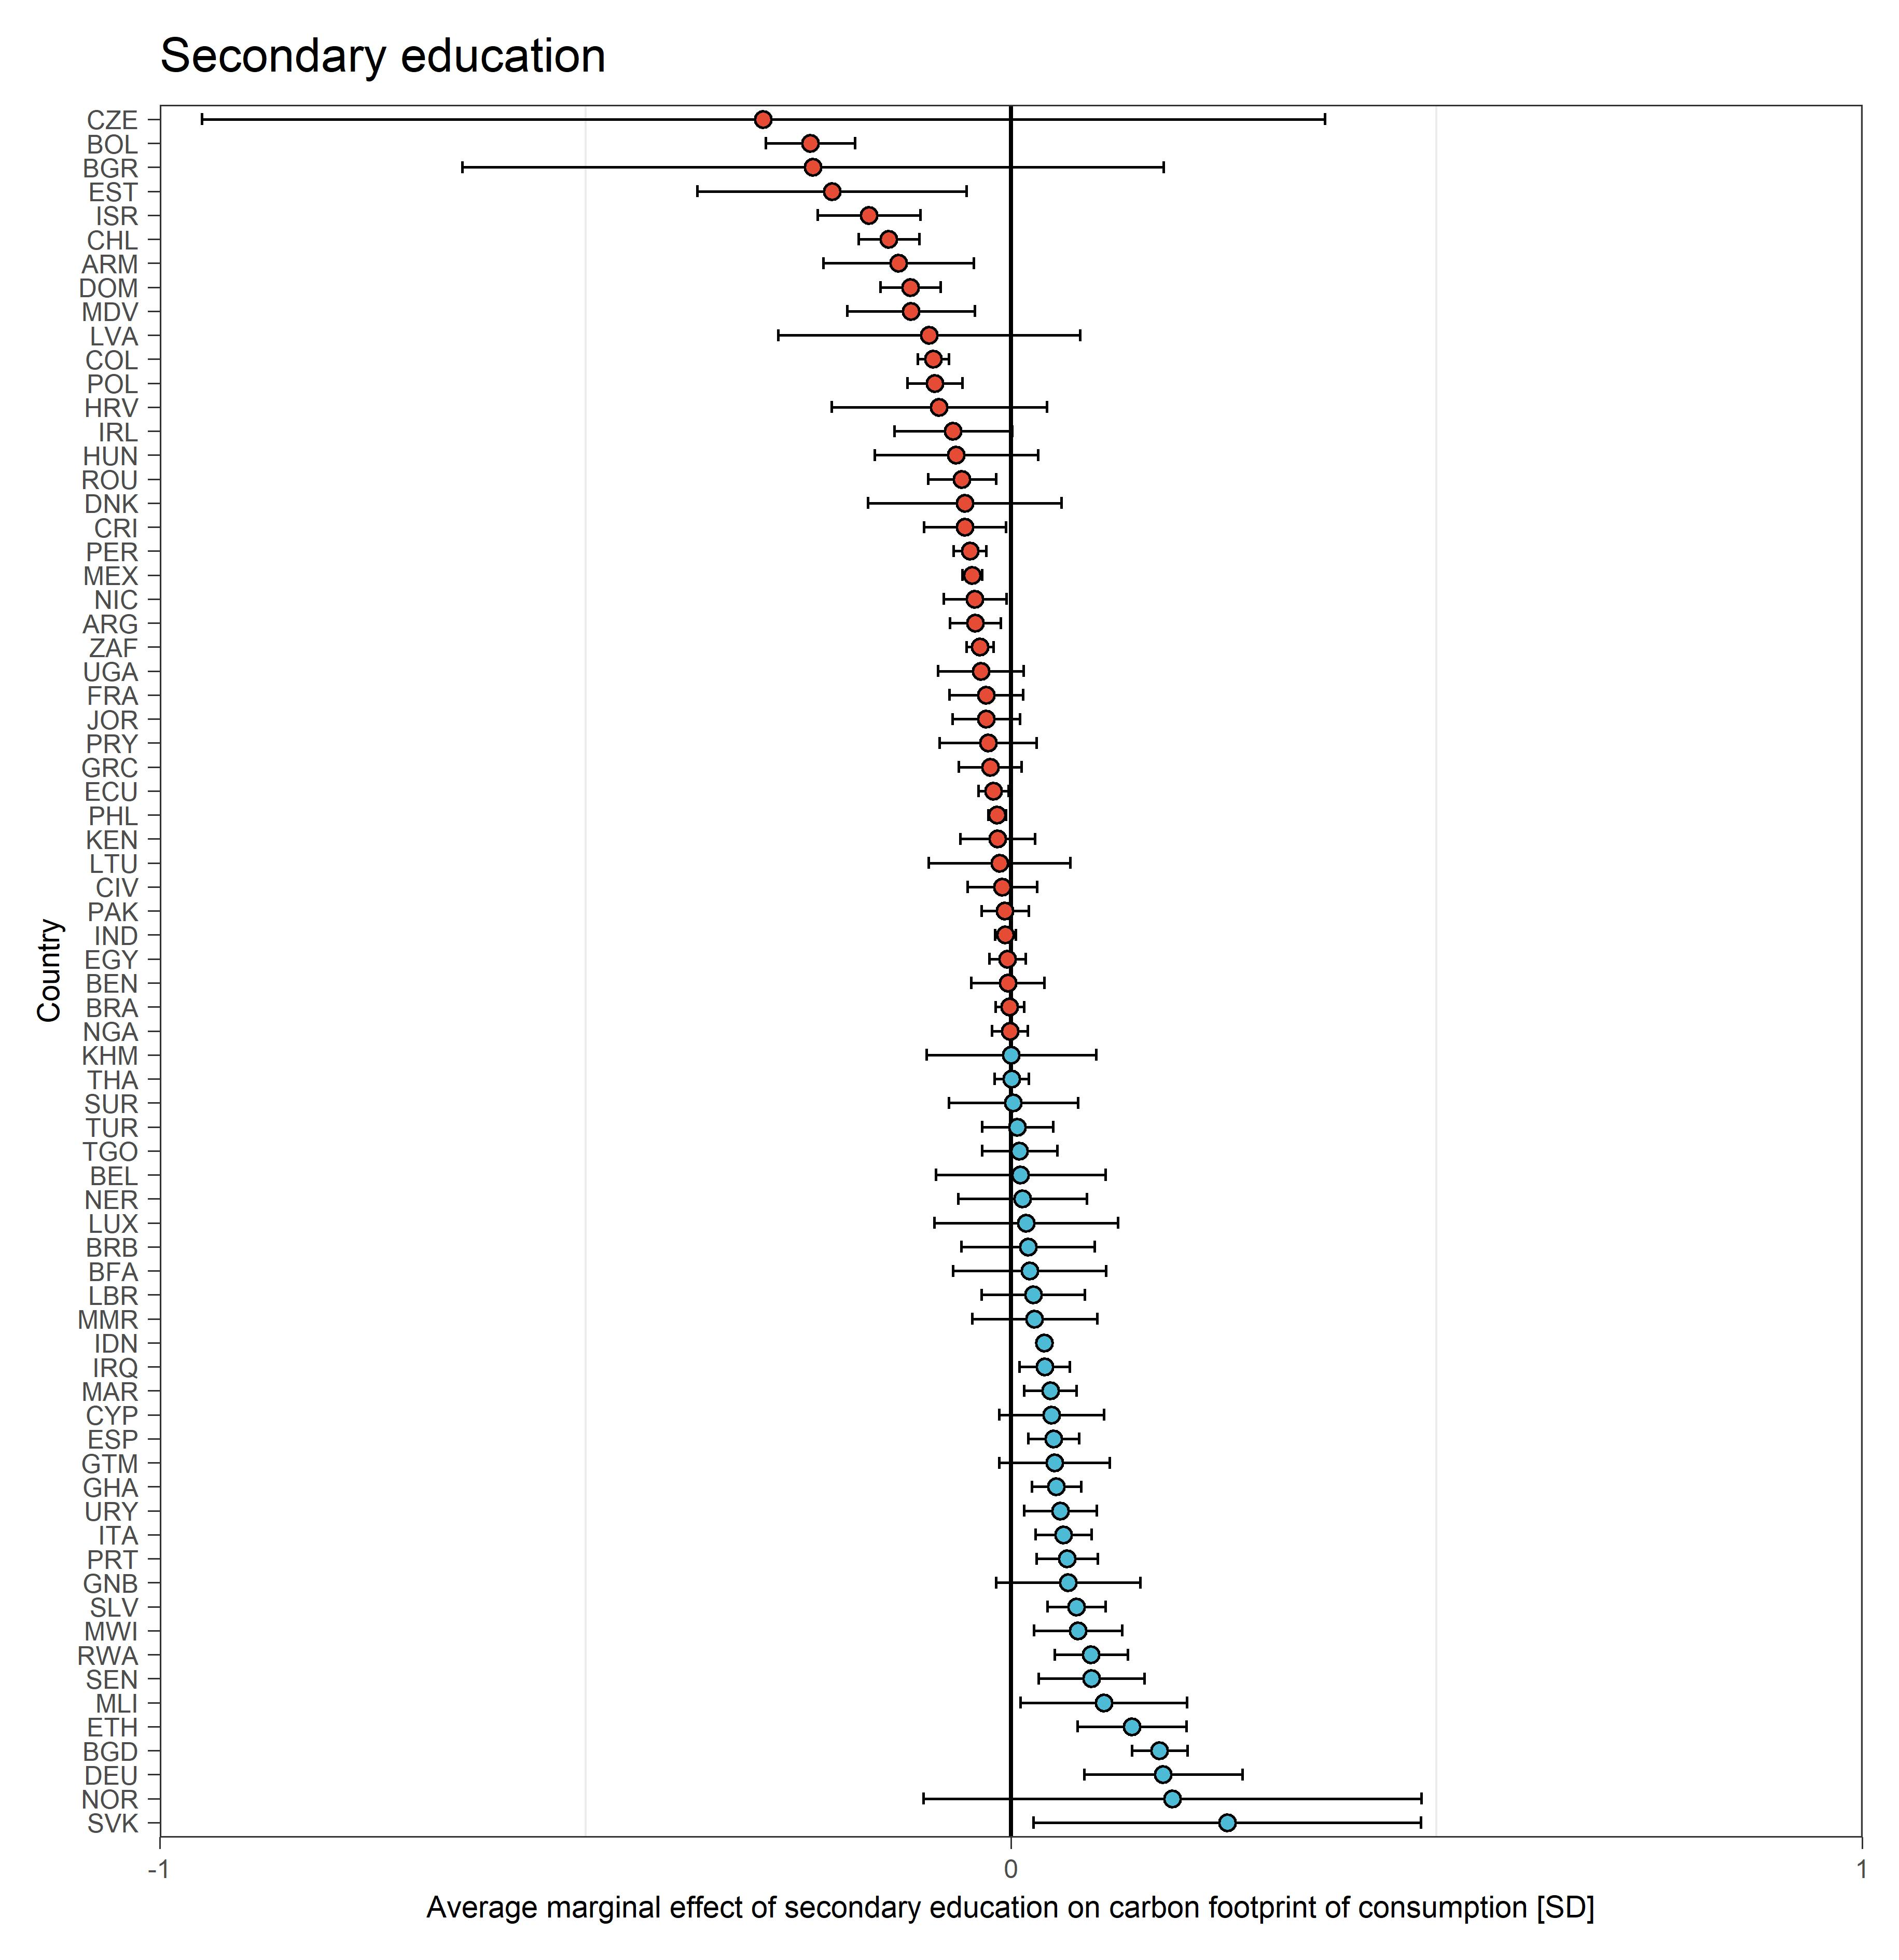
\includegraphics{Analysis_OLS_ME_Carbon_Footprint/AME_OLS_FP_secondary_education}
%   \begin{subcaption}
%     This figure displays ... Finland special case
%   \end{subcaption}

% \end{figure}

% \clearpage

% \begin{figure}[ht!]
%   \centering
%  \caption{Average marginal effects of higher education} \label{fig:D11_high_edu}
%   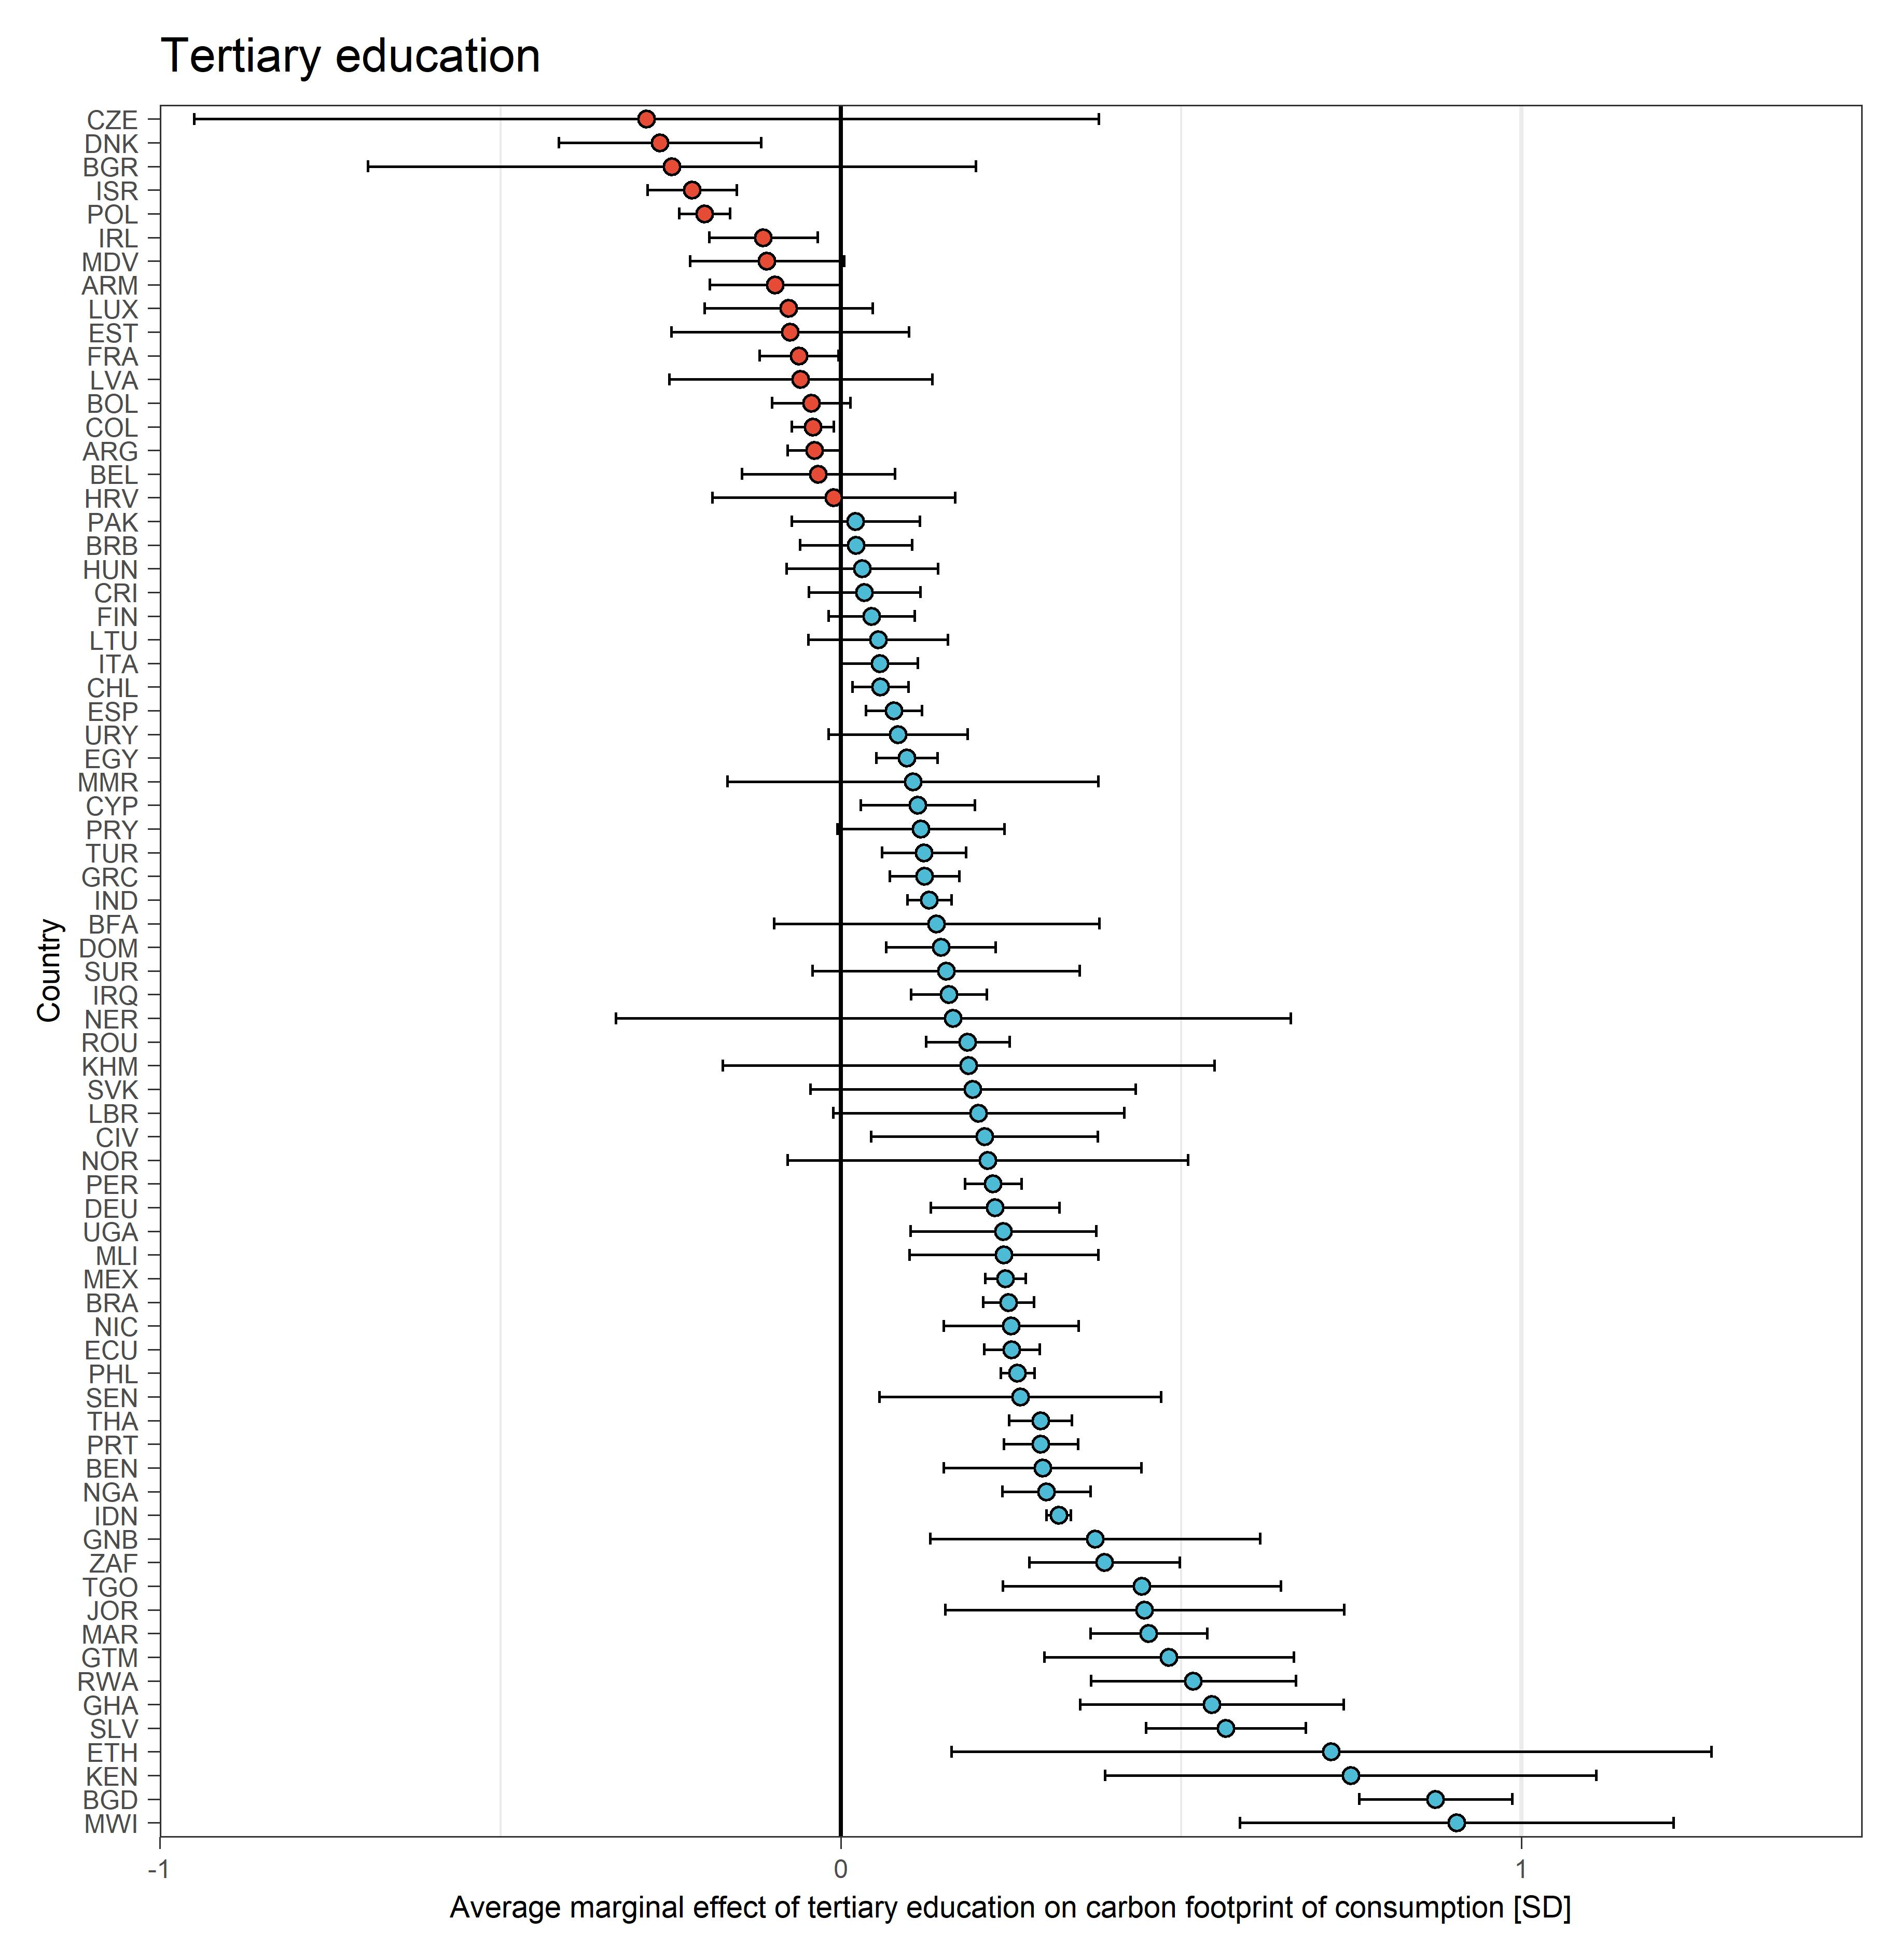
\includegraphics{Analysis_OLS_ME_Carbon_Footprint/AME_OLS_FP_higher_education}
%   \begin{subcaption}
%     This figure displays ... Finland special case
%   \end{subcaption}

% \end{figure}

% \clearpage

% \begin{figure}[ht!]
%   \centering
%  \caption{Average marginal effects of car ownership} \label{fig:E1_Car}
%   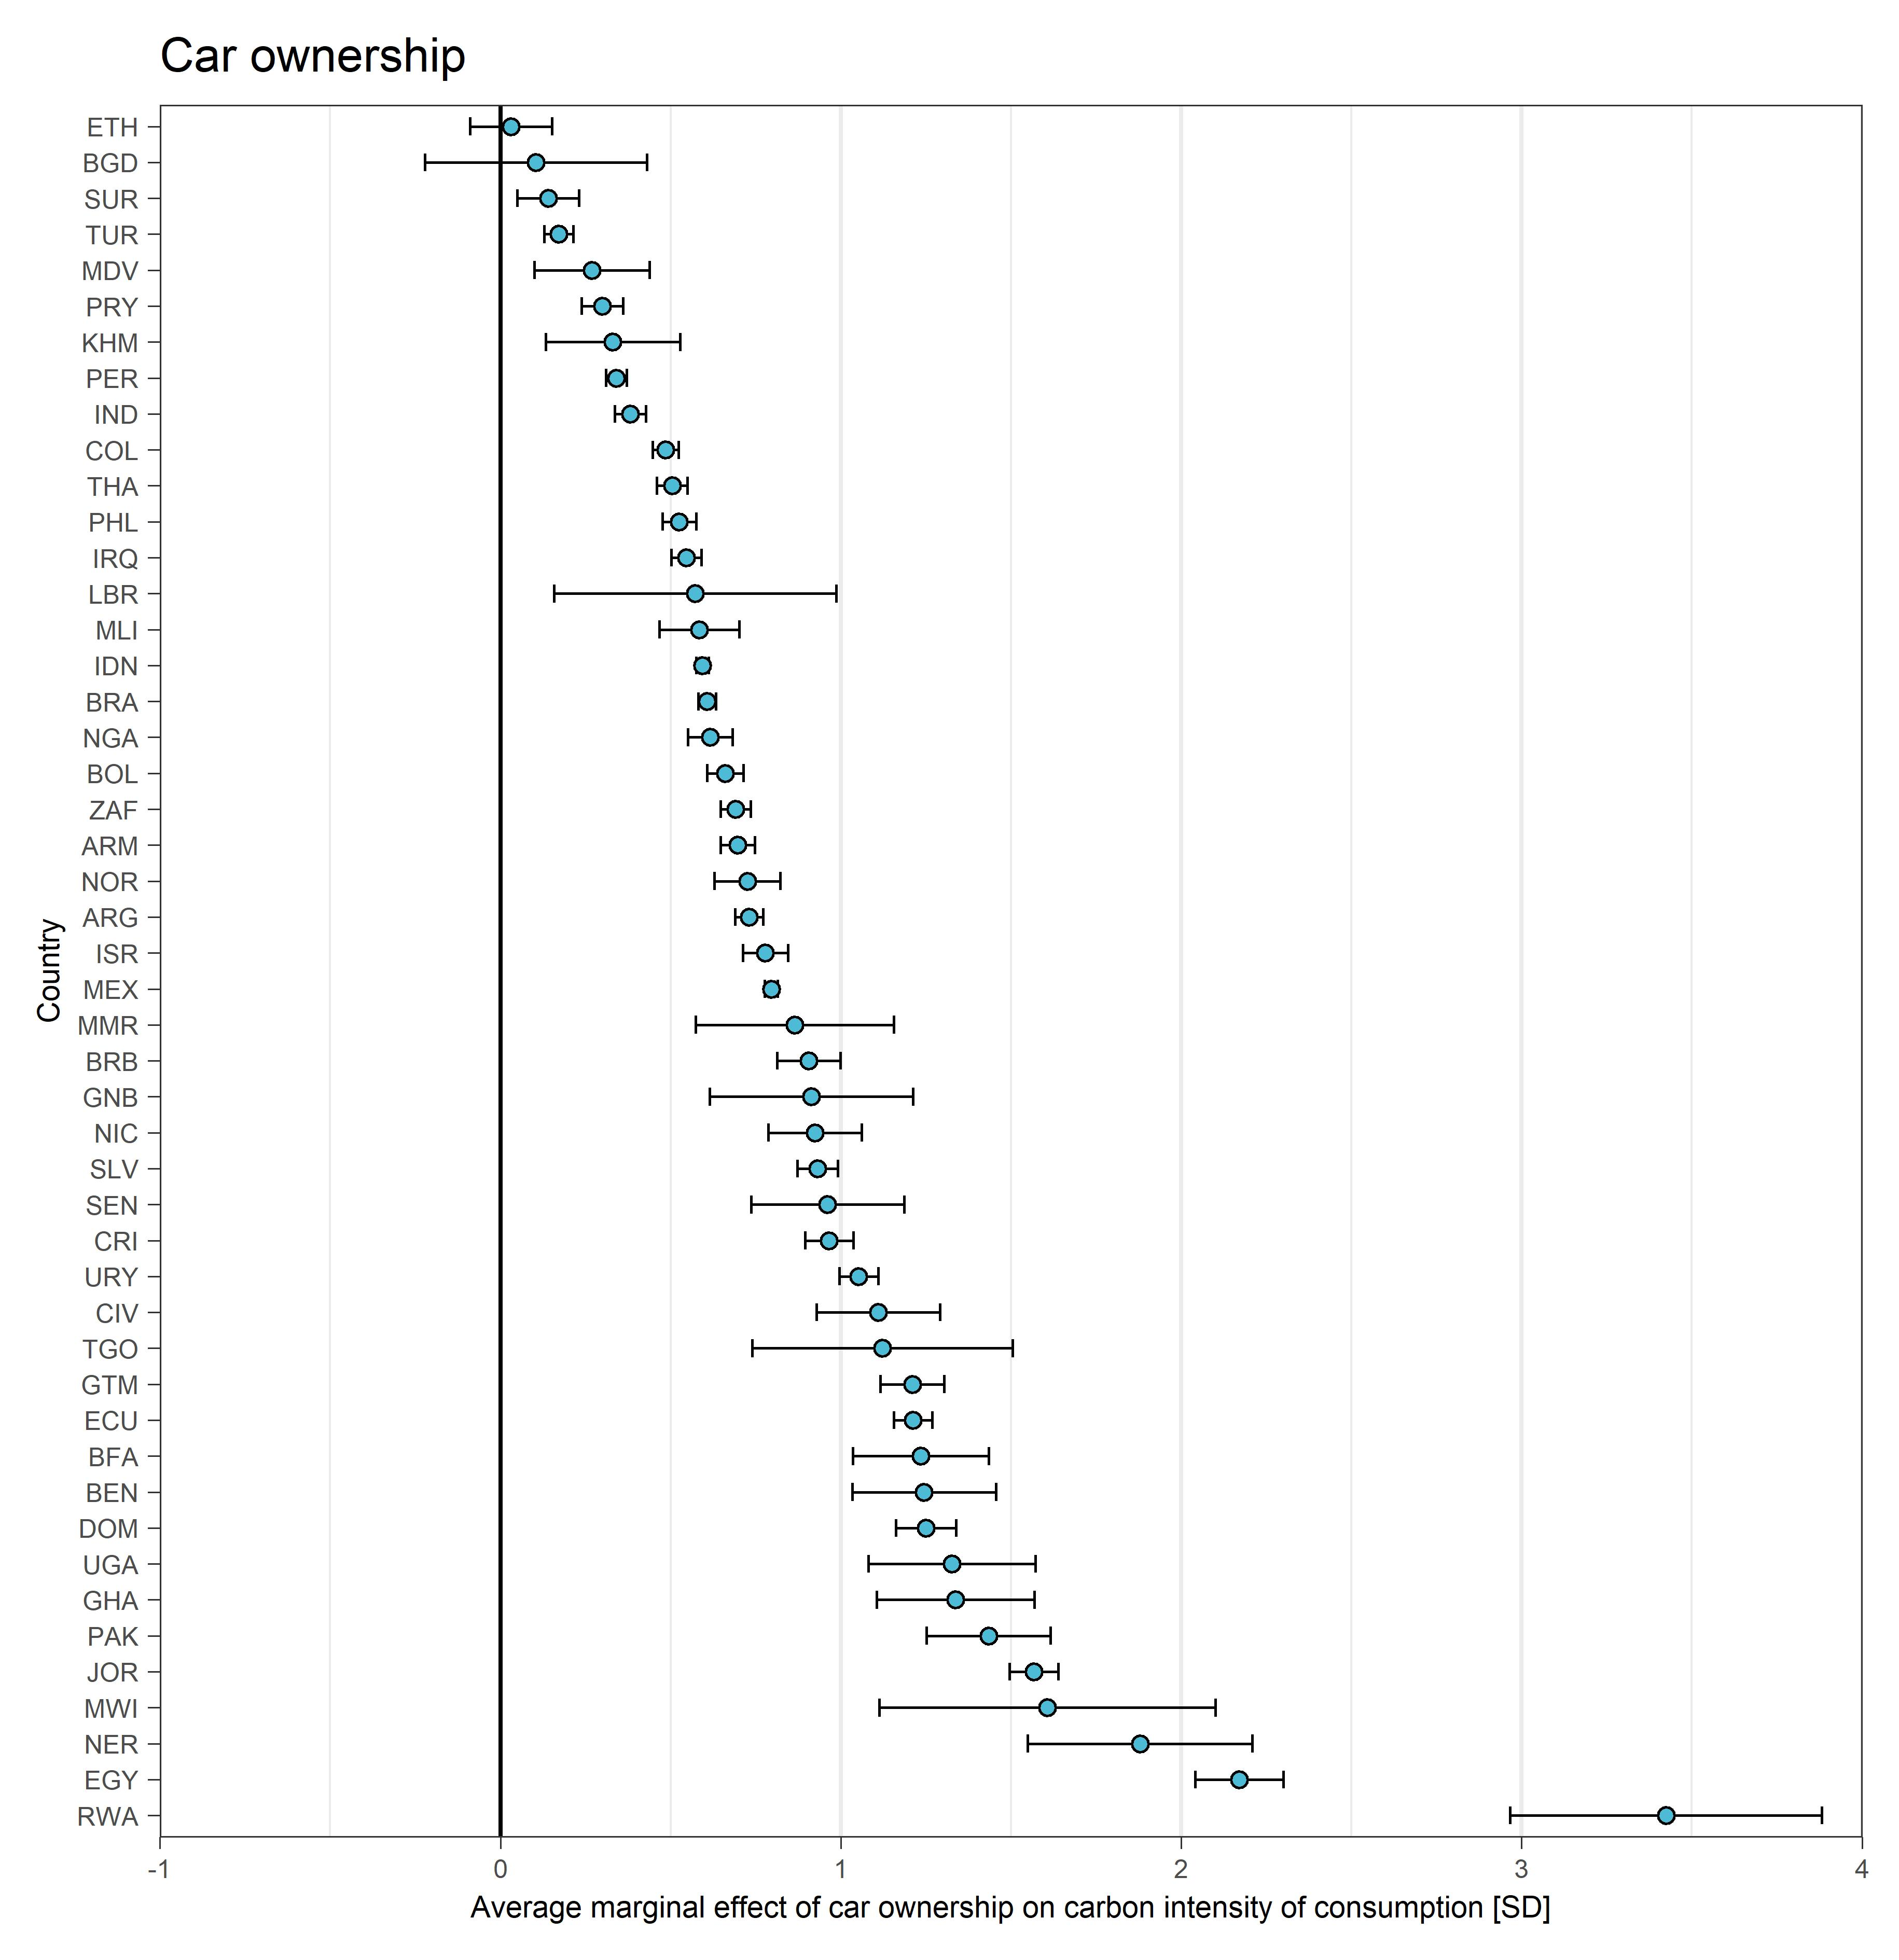
\includegraphics{Analysis_OLS_ME_Carbon_Intensity/AME_OLS_CI_car.01}
%   \begin{subcaption}
%     This figure displays ...
%   \end{subcaption}

% \end{figure}

% \clearpage

% \begin{figure}[ht!]
%   \centering
%  \caption{Average marginal effects of electricity access} \label{fig:E2_Electricity}
%   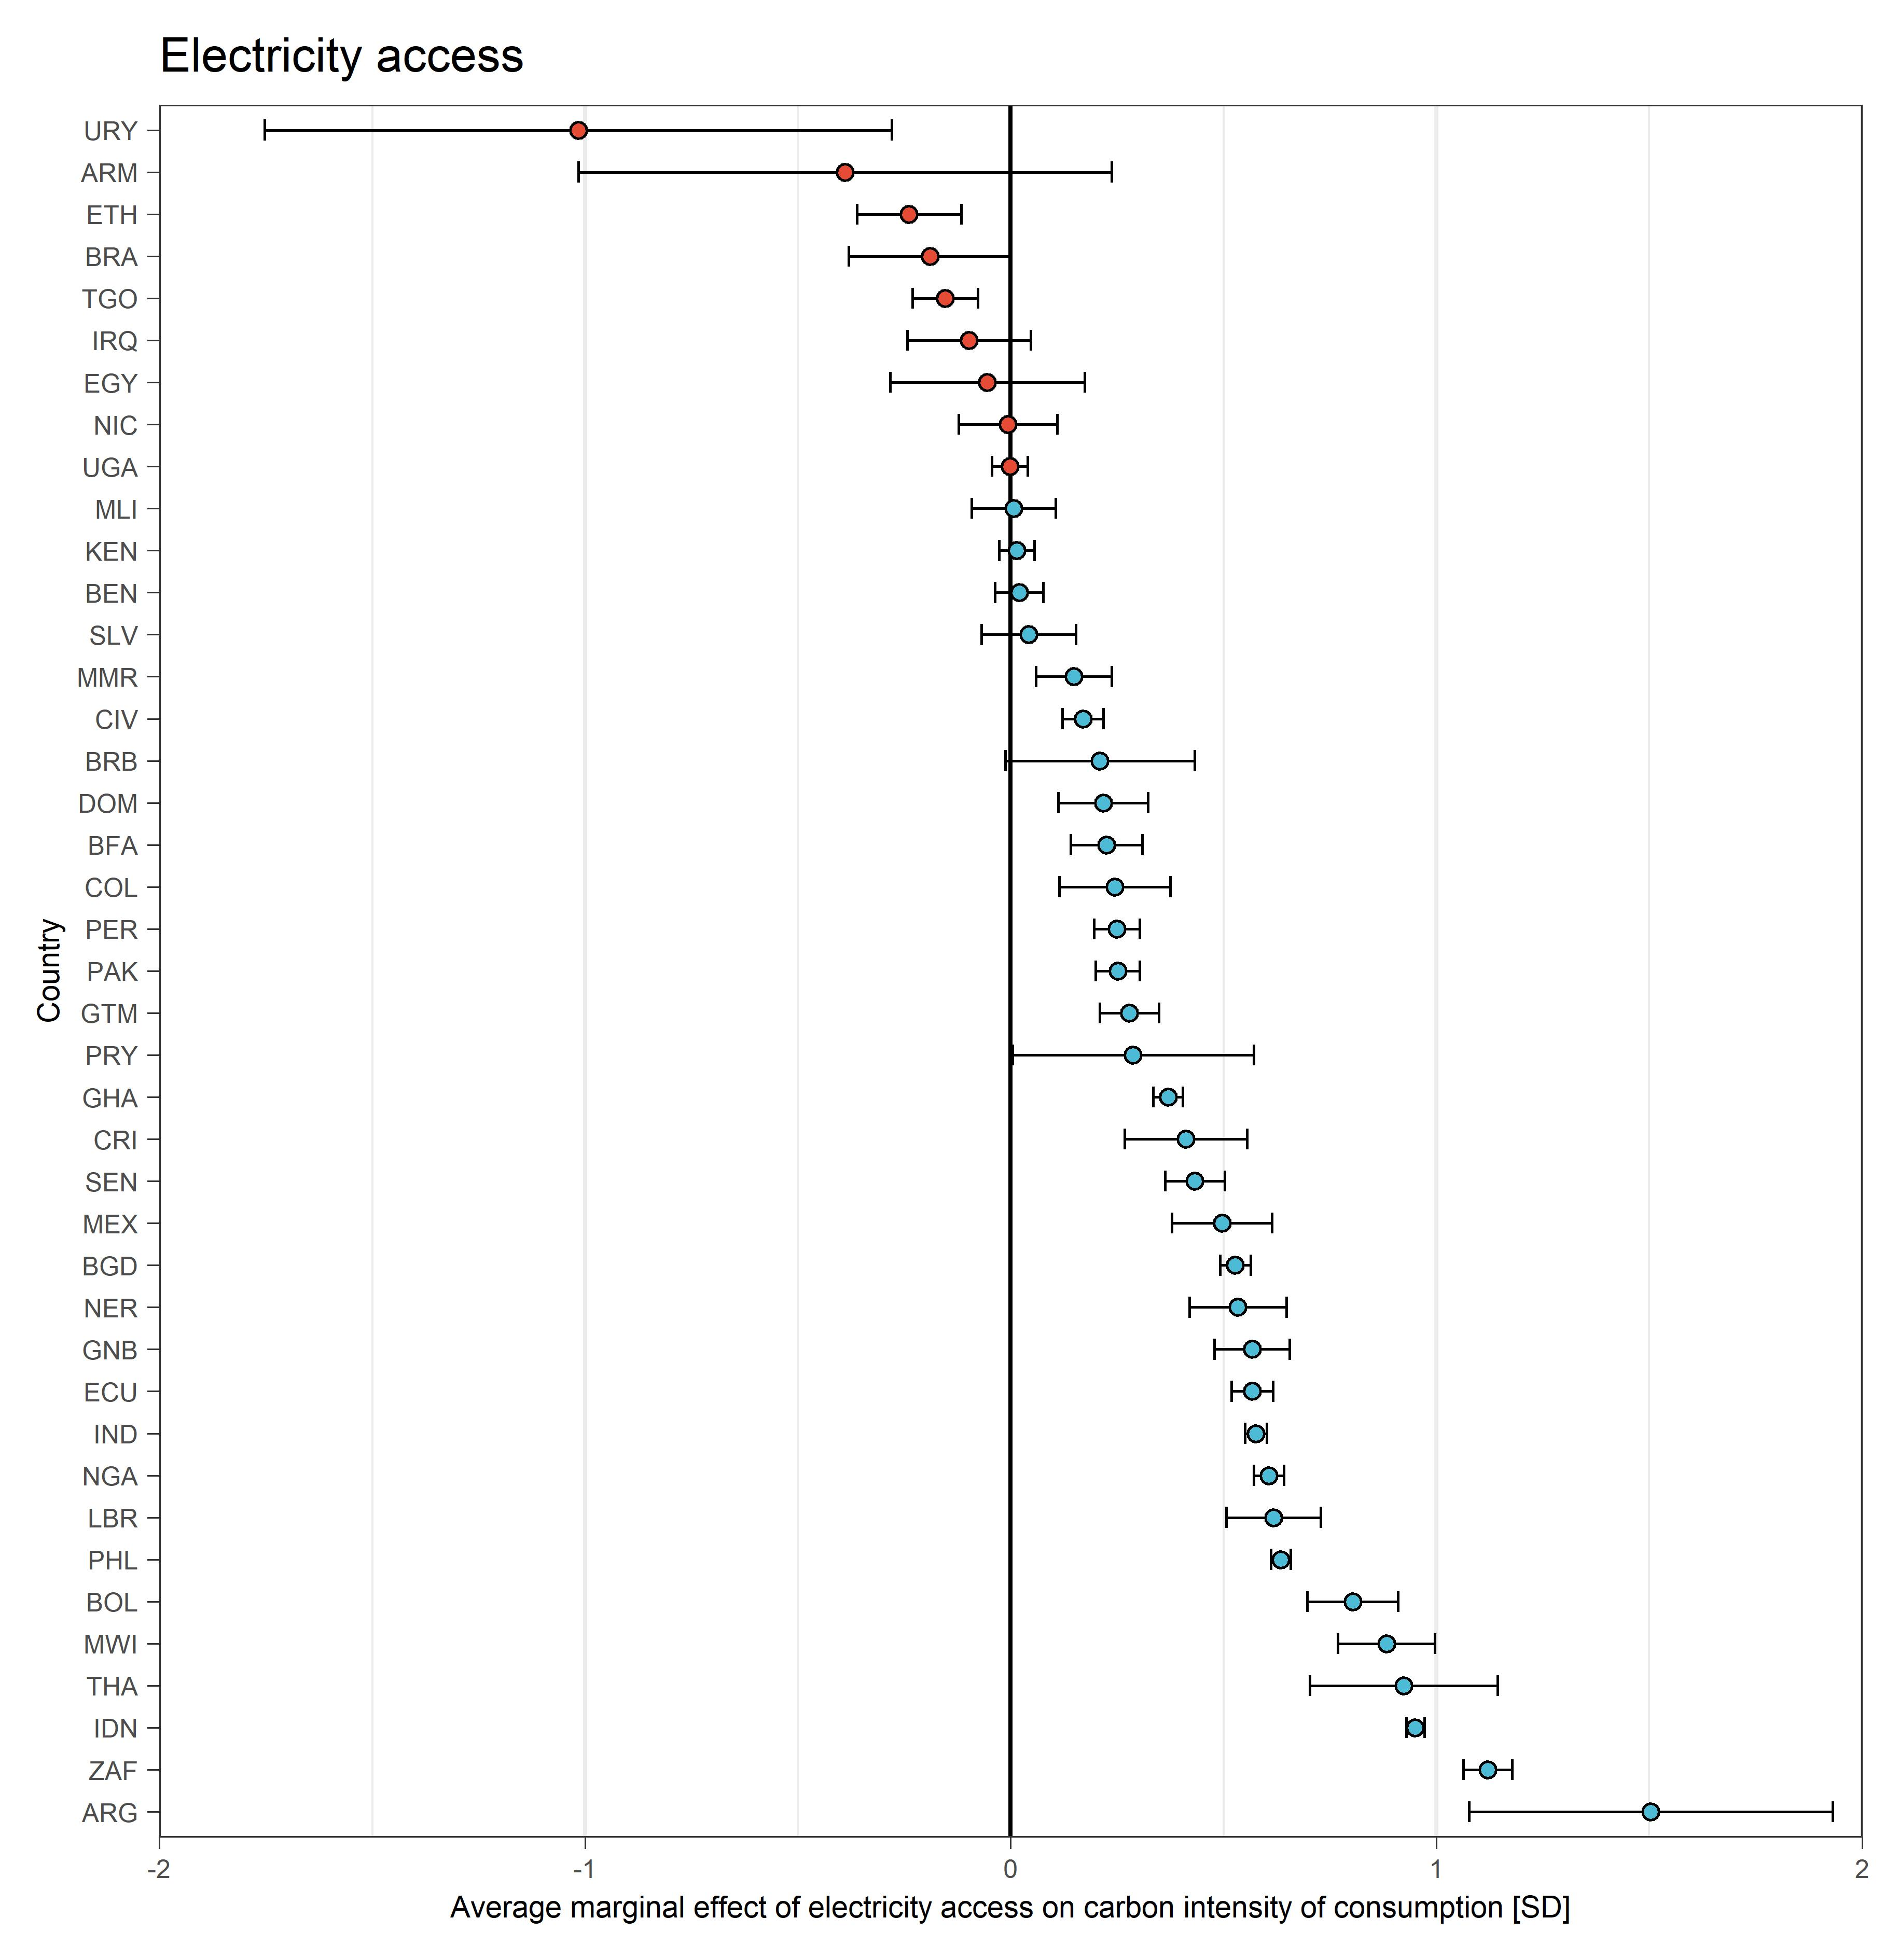
\includegraphics{Analysis_OLS_ME_Carbon_Intensity/AME_OLS_CI_electricity.access}
%   \begin{subcaption}
%     This figure displays ...
%   \end{subcaption}

% \end{figure}

% \clearpage

% \begin{figure}[ht!]
%   \centering
%  \caption{Average marginal effects of household size} \label{fig:E3_Size}
%   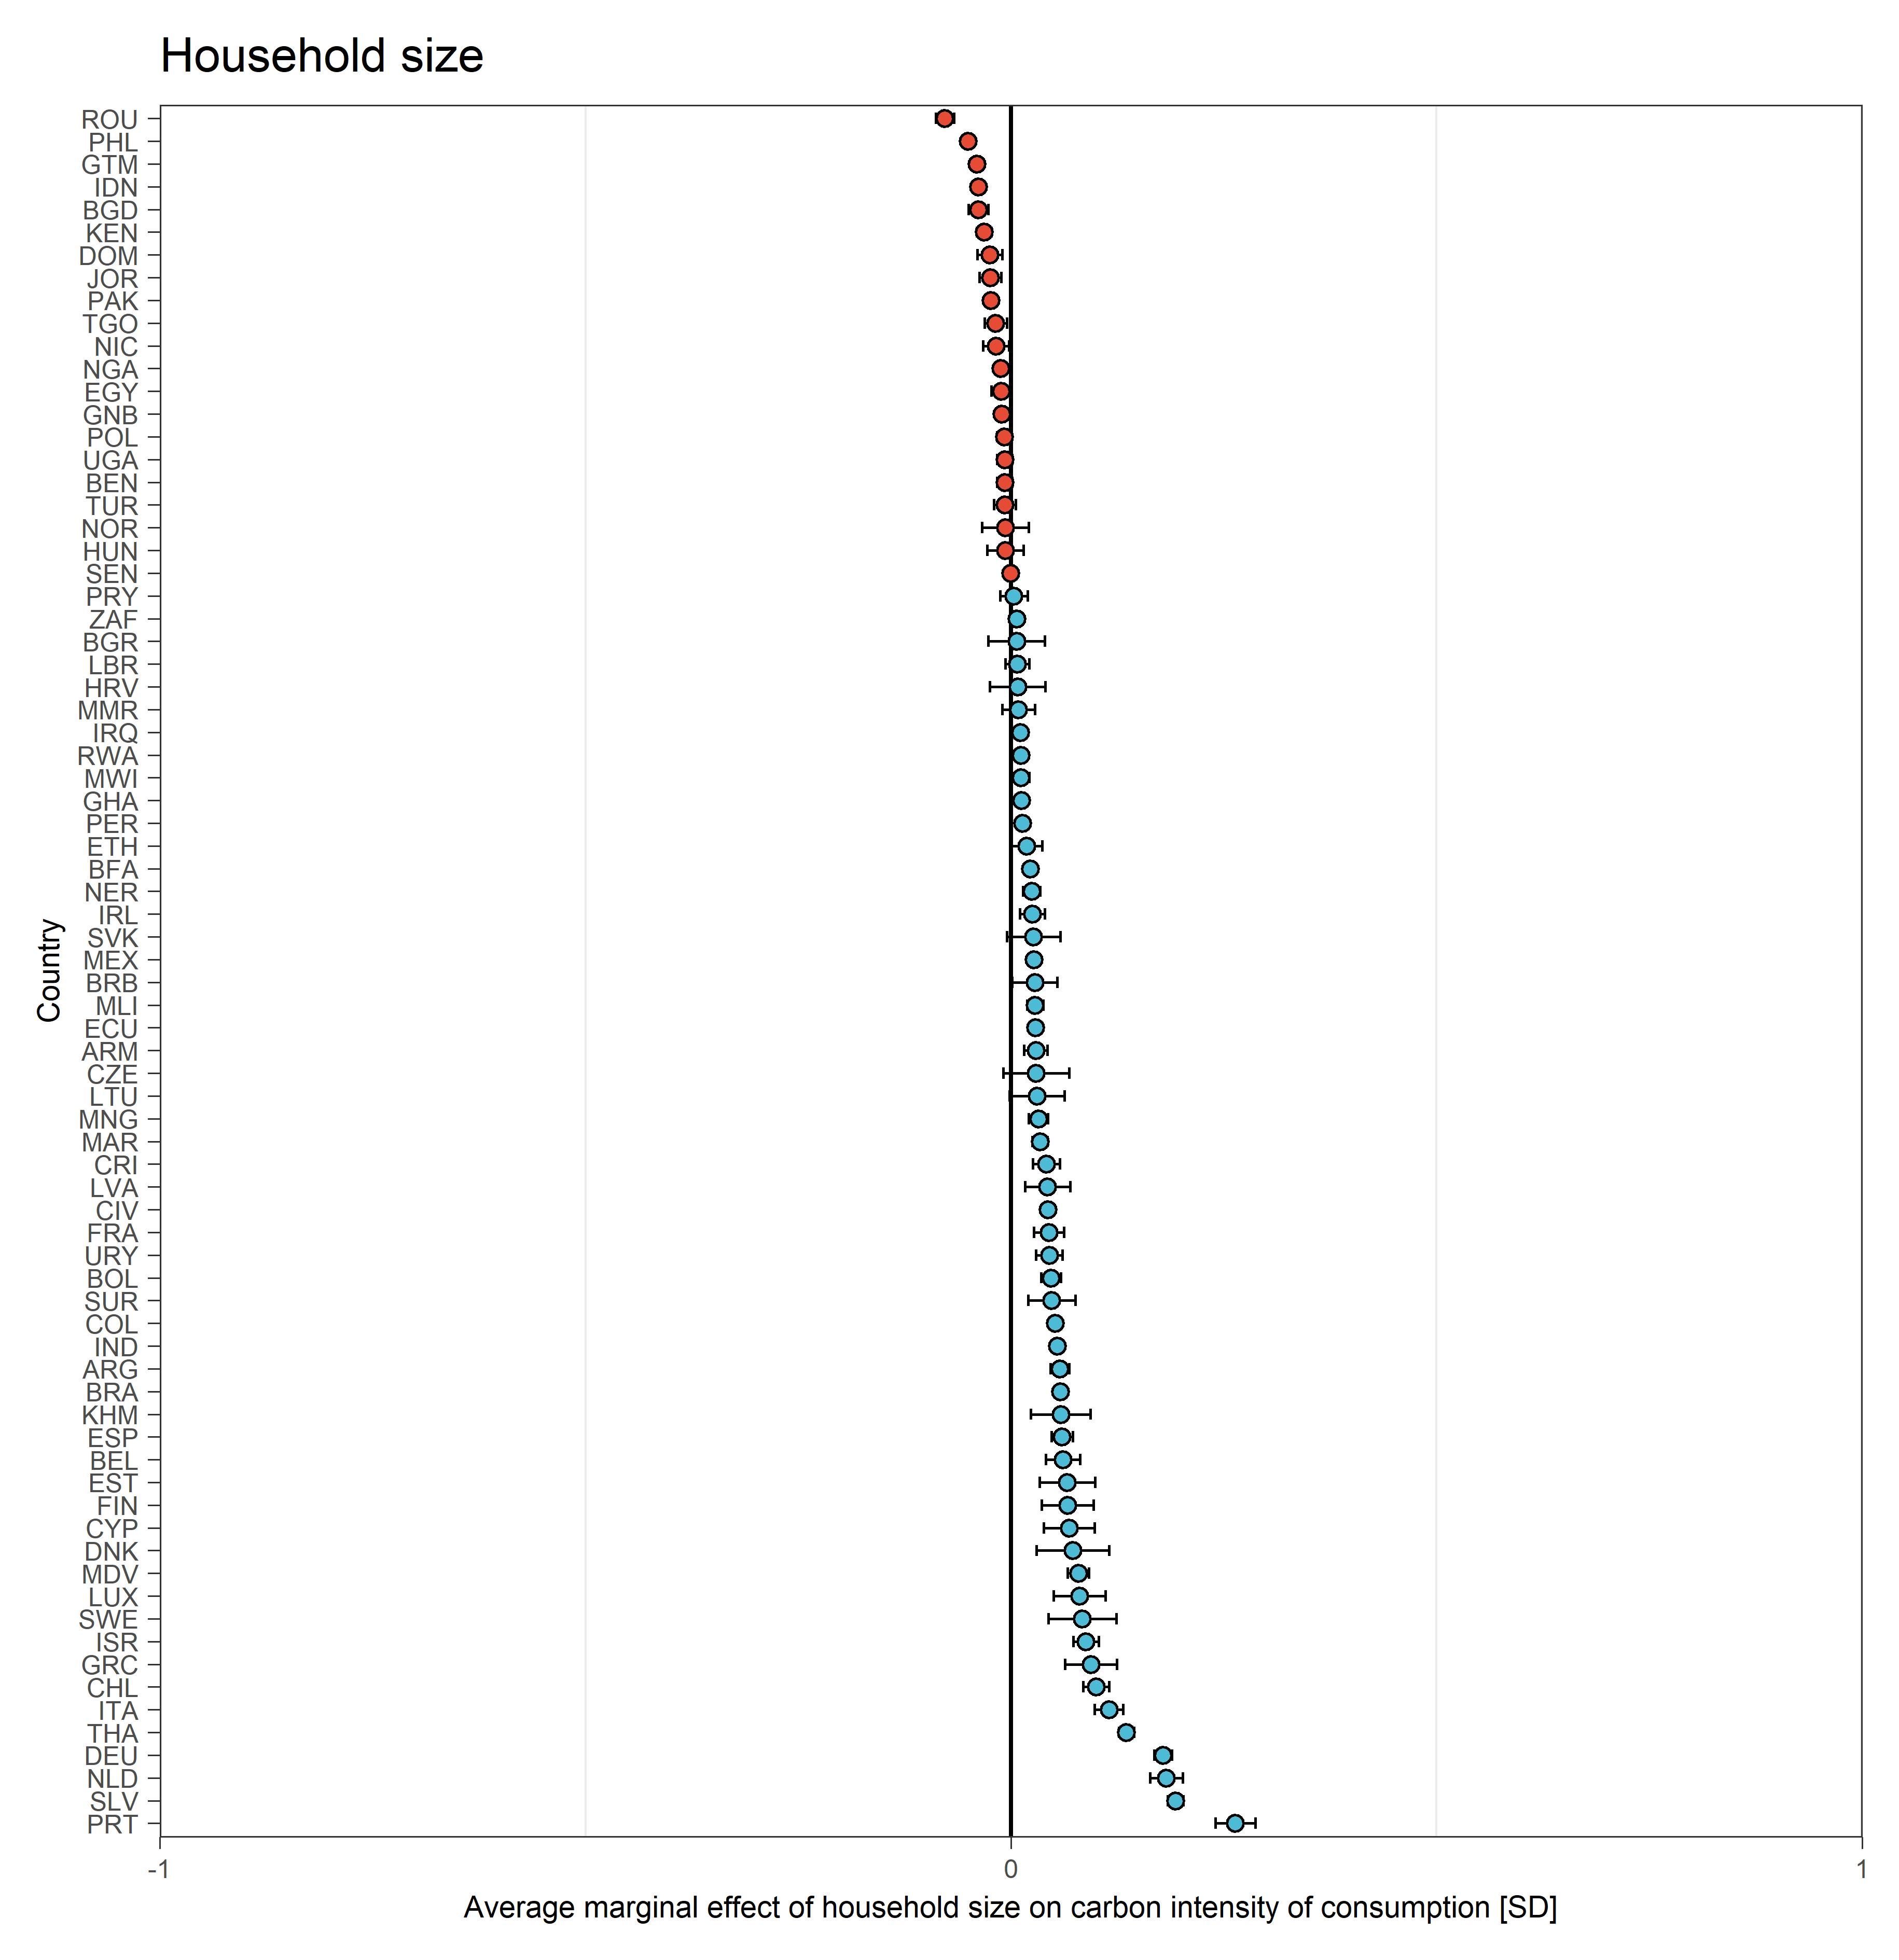
\includegraphics{Analysis_OLS_ME_Carbon_Intensity/AME_OLS_CI_hh_size}
%   \begin{subcaption}
%     This figure displays ...
%   \end{subcaption}

% \end{figure}

% \clearpage

% \begin{figure}[ht!]
%   \centering
%  \caption{Average marginal effects of household expenditures} \label{fig:E4_Expenditures}
%   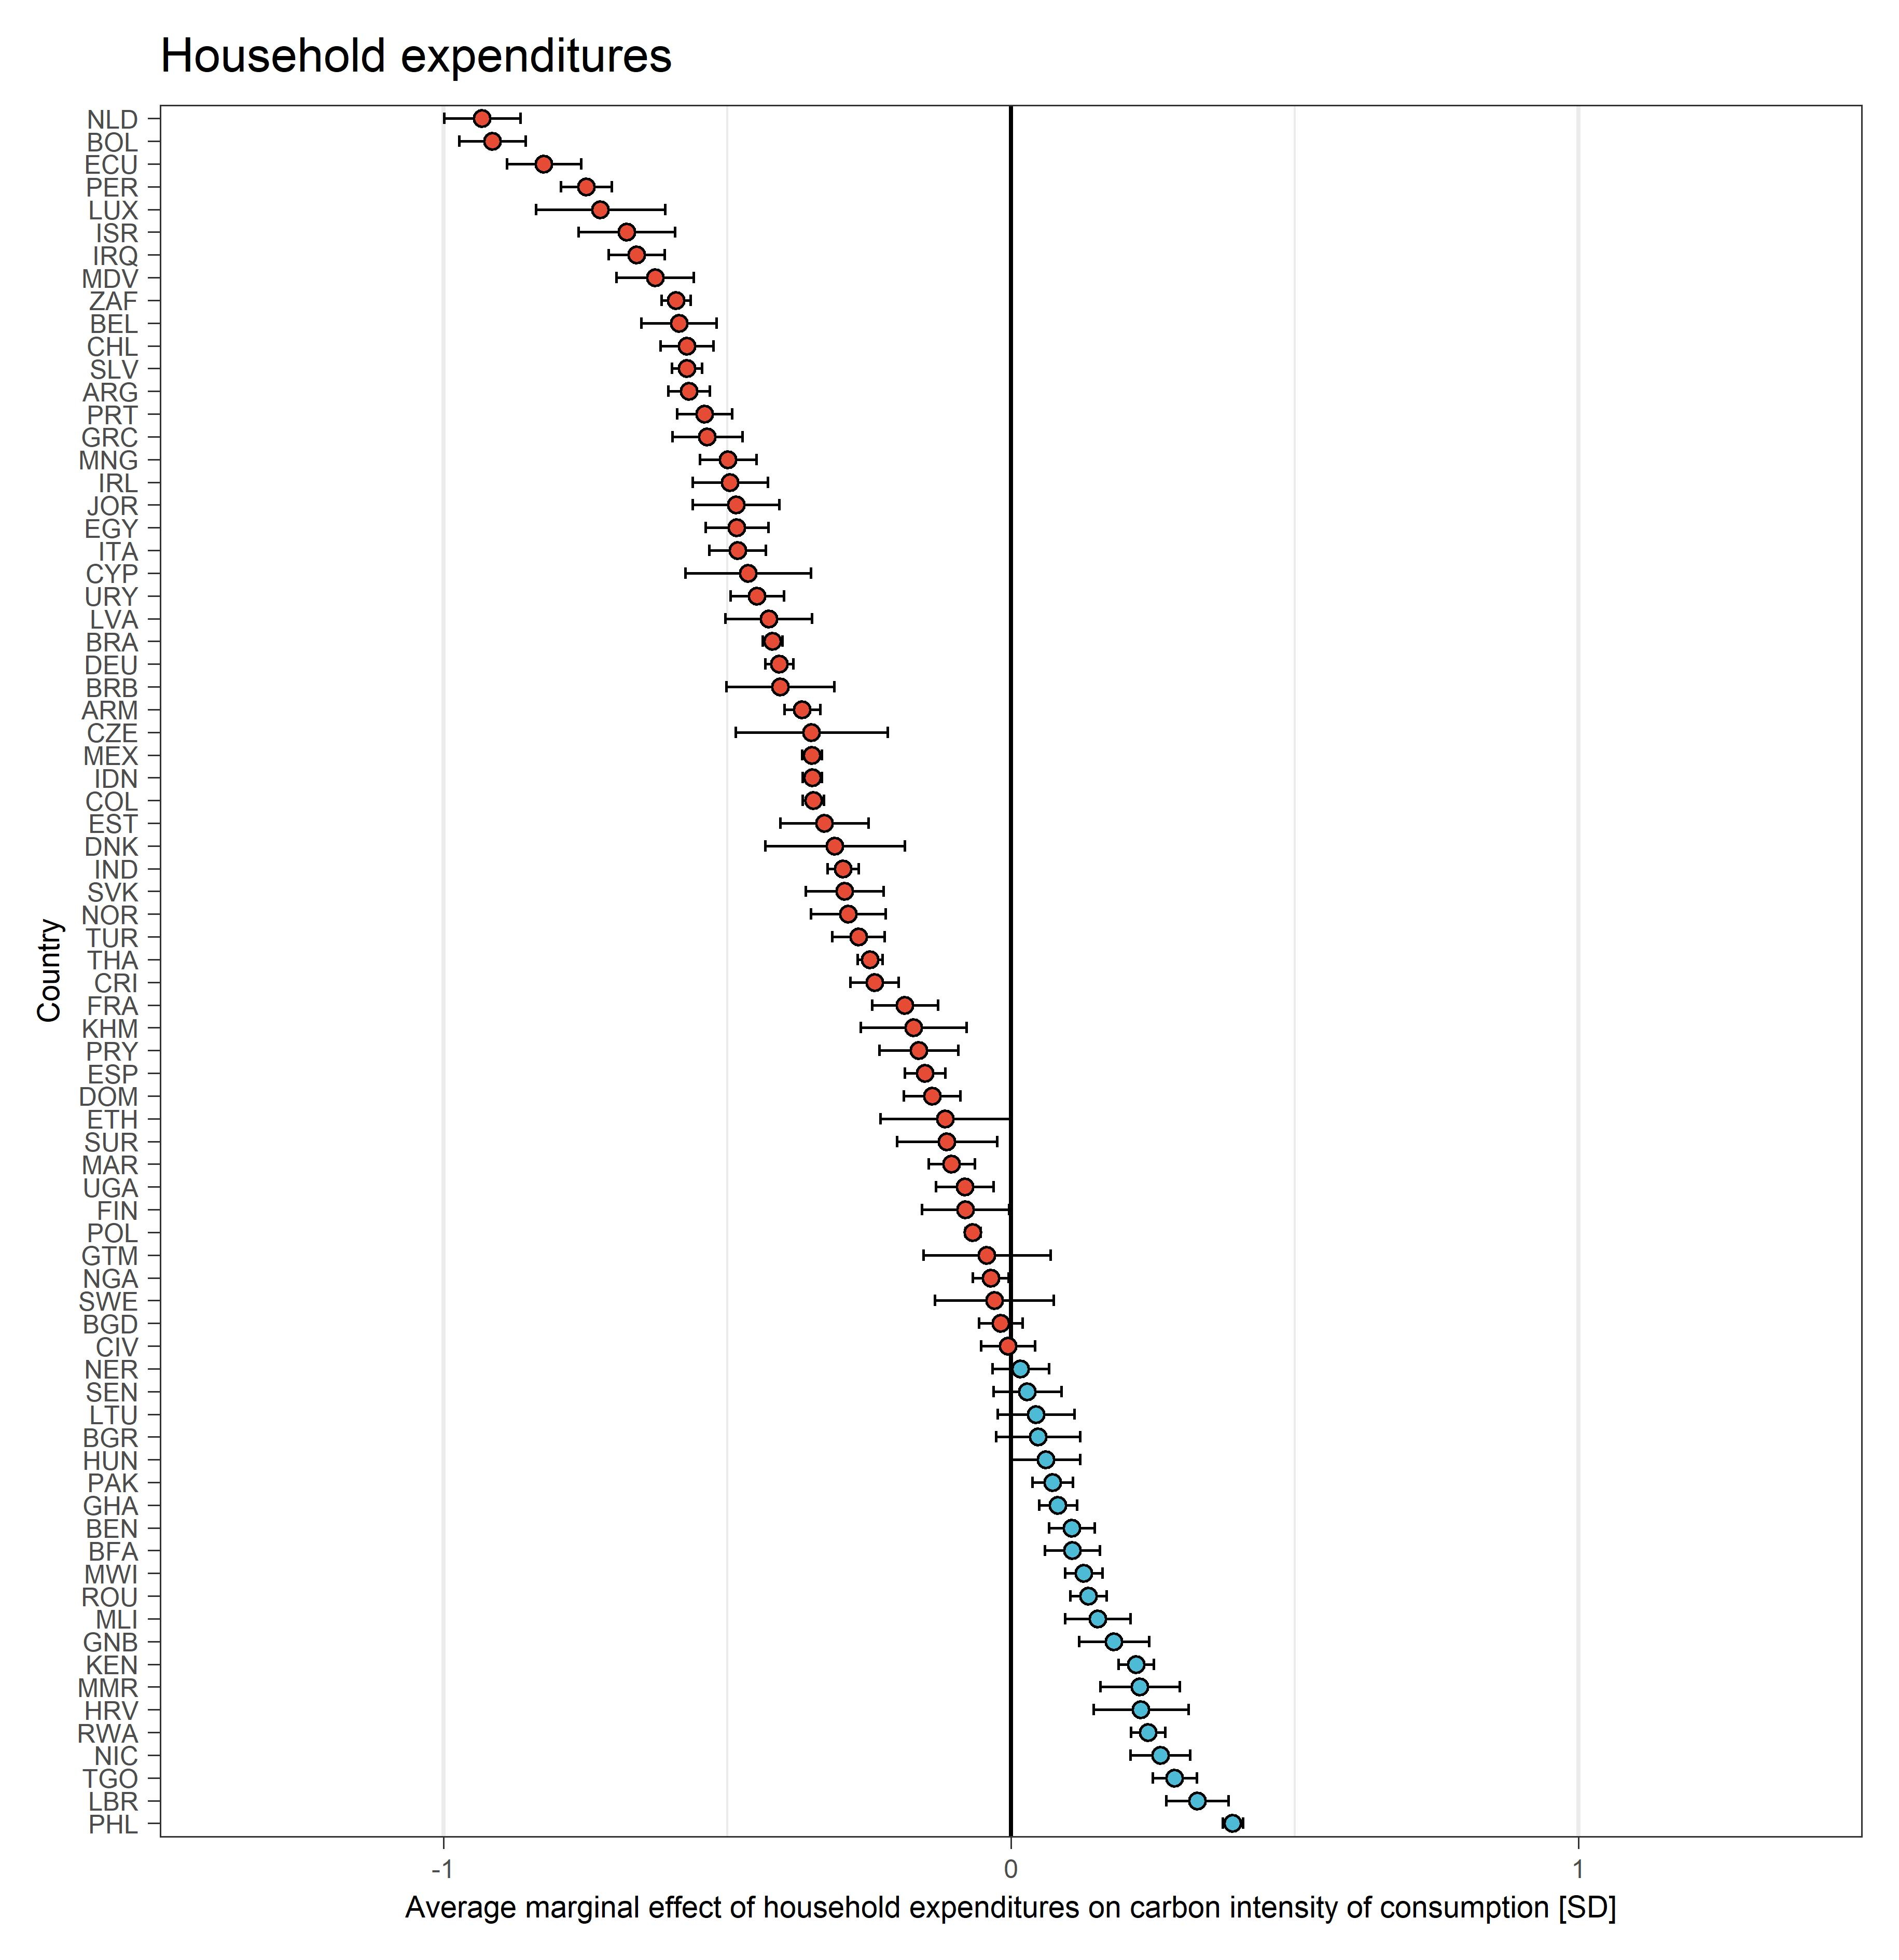
\includegraphics{Analysis_OLS_ME_Carbon_Intensity/AME_OLS_CI_log_hh_expenditures_USD_2014}
%   \begin{subcaption}
%     This figure displays ...
%   \end{subcaption}

% \end{figure}

% \clearpage

% \begin{figure}[ht!]
%   \centering
%  \caption{Average marginal effects of urban citizenship} \label{fig:E5_Urban}
%   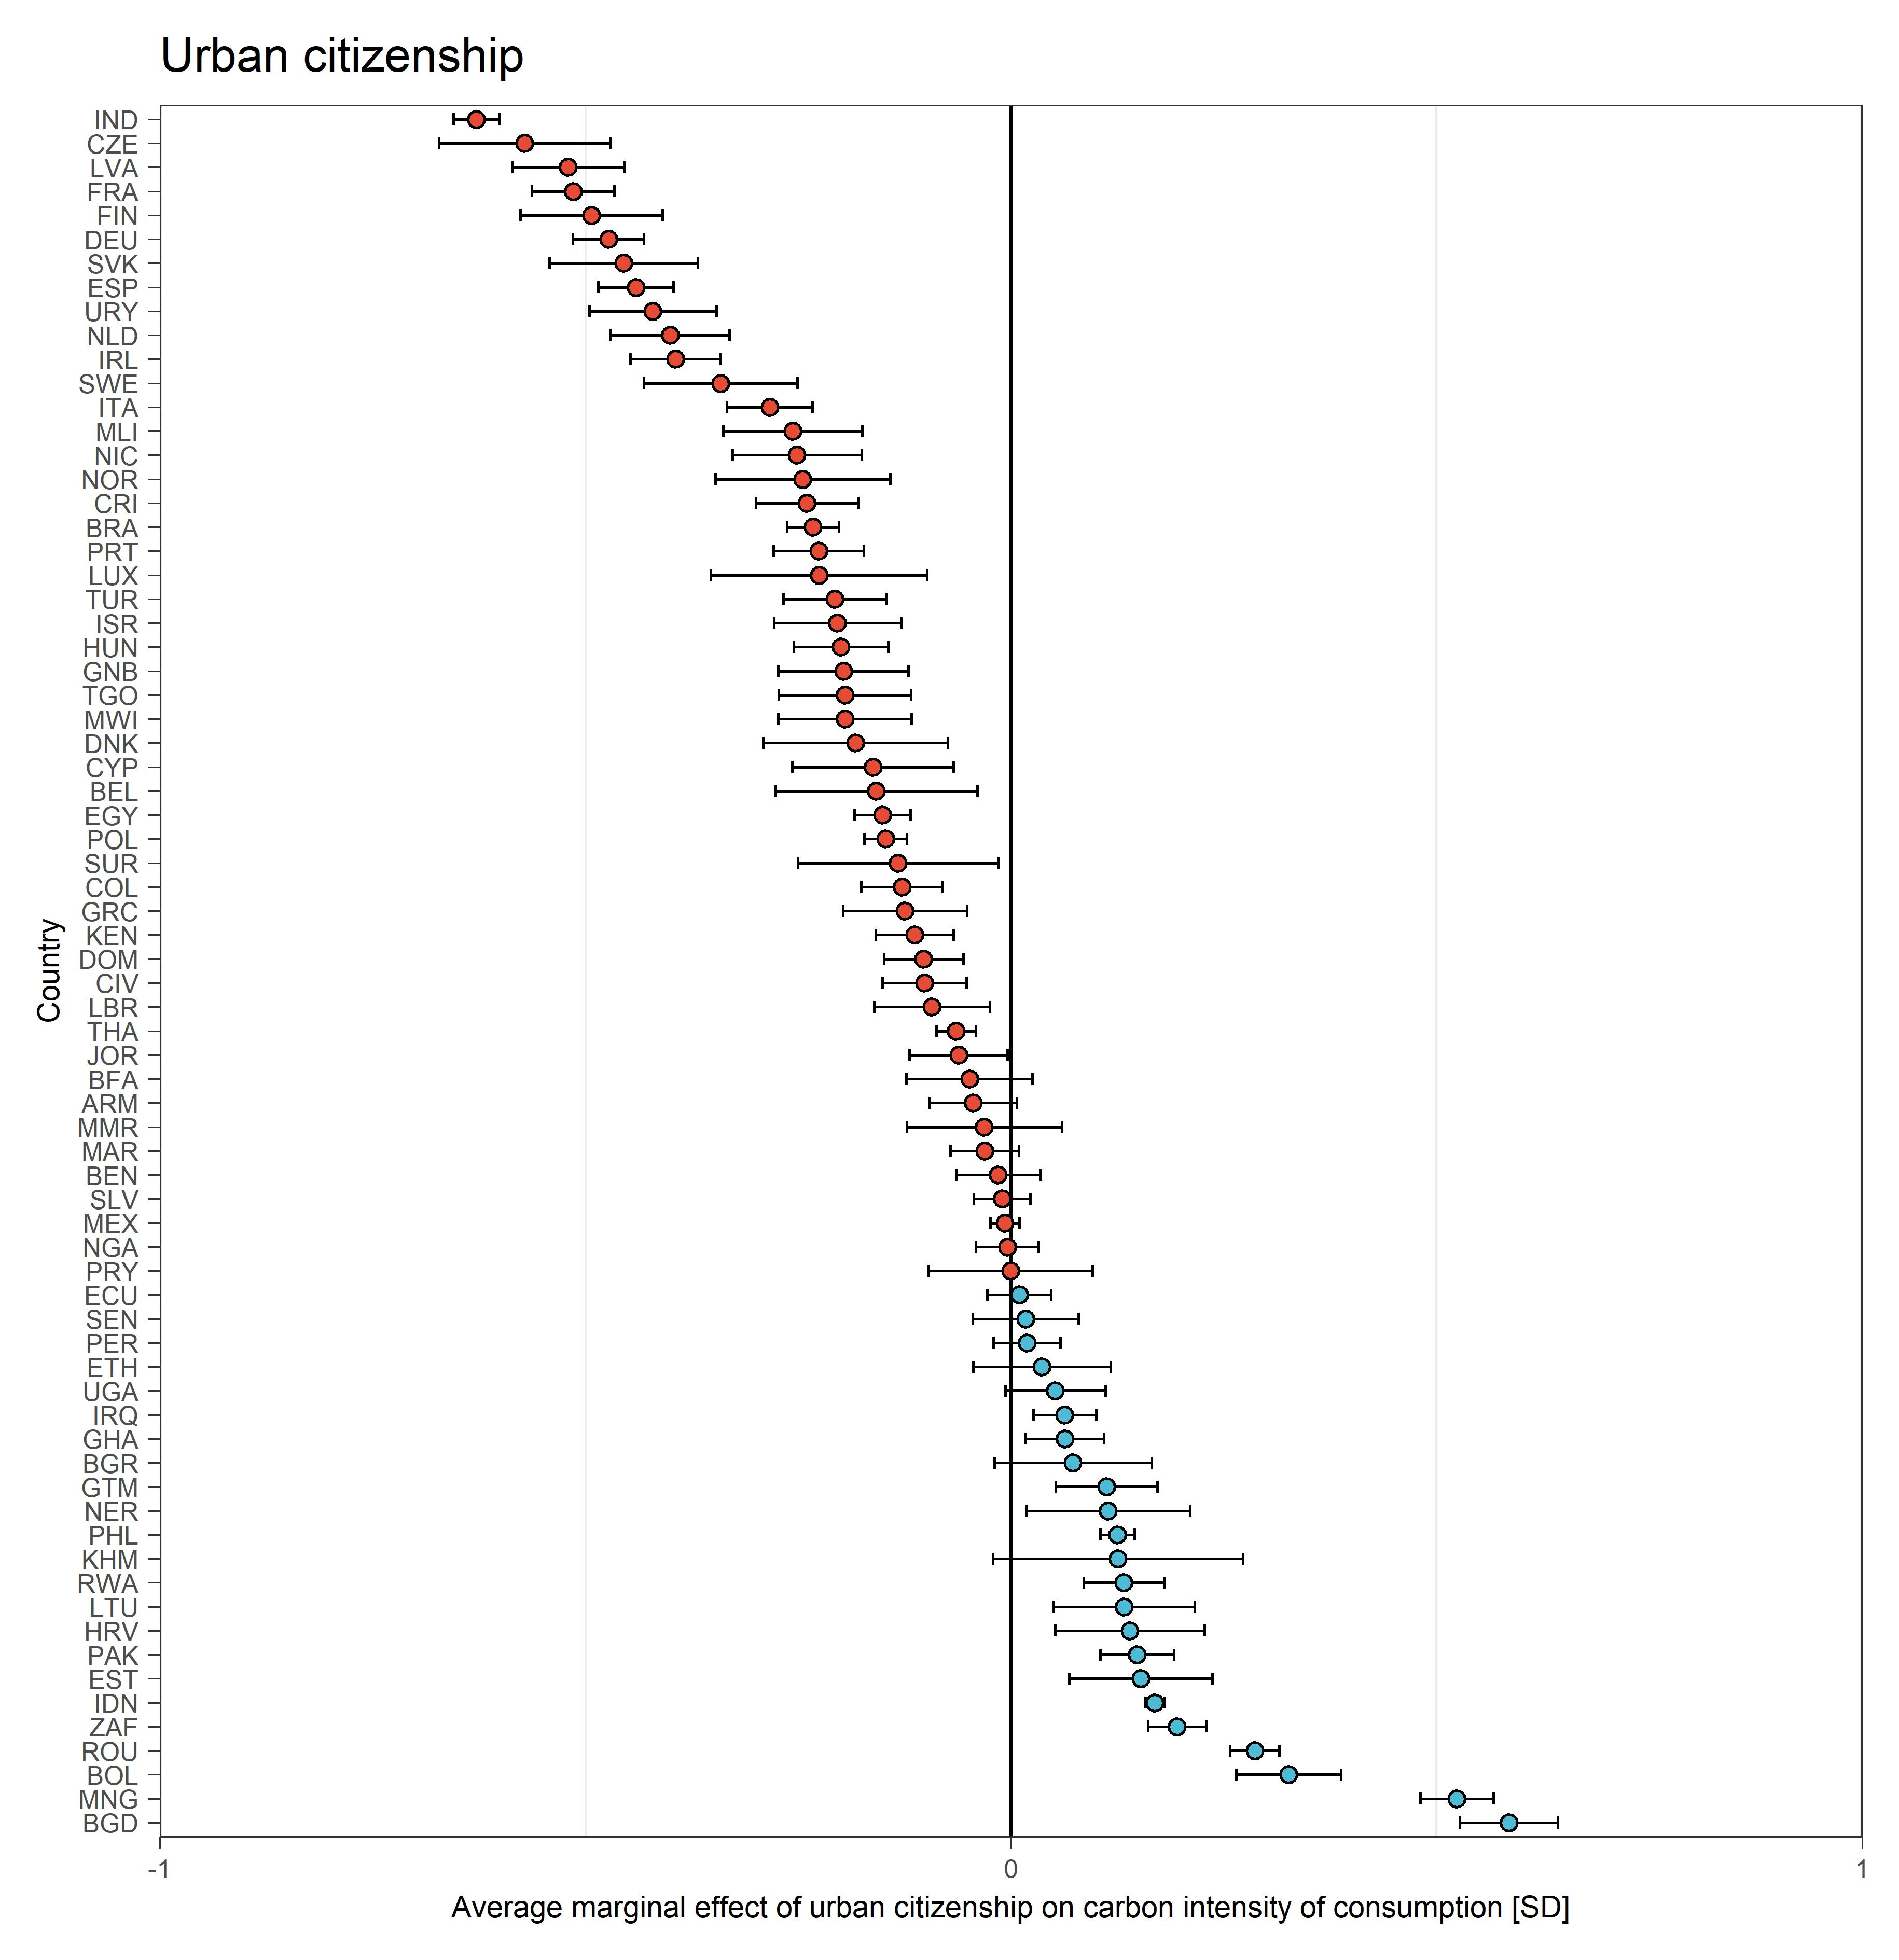
\includegraphics{Analysis_OLS_ME_Carbon_Intensity/AME_OLS_CI_urban_01}
%   \begin{subcaption}
%     This figure displays ...
%   \end{subcaption}

% \end{figure}

% \clearpage

% \begin{figure}[ht!]
%   \centering
%  \caption{Average marginal effects of cooking fuel choice - Part A} \label{fig:E6_Electricity_A}
%   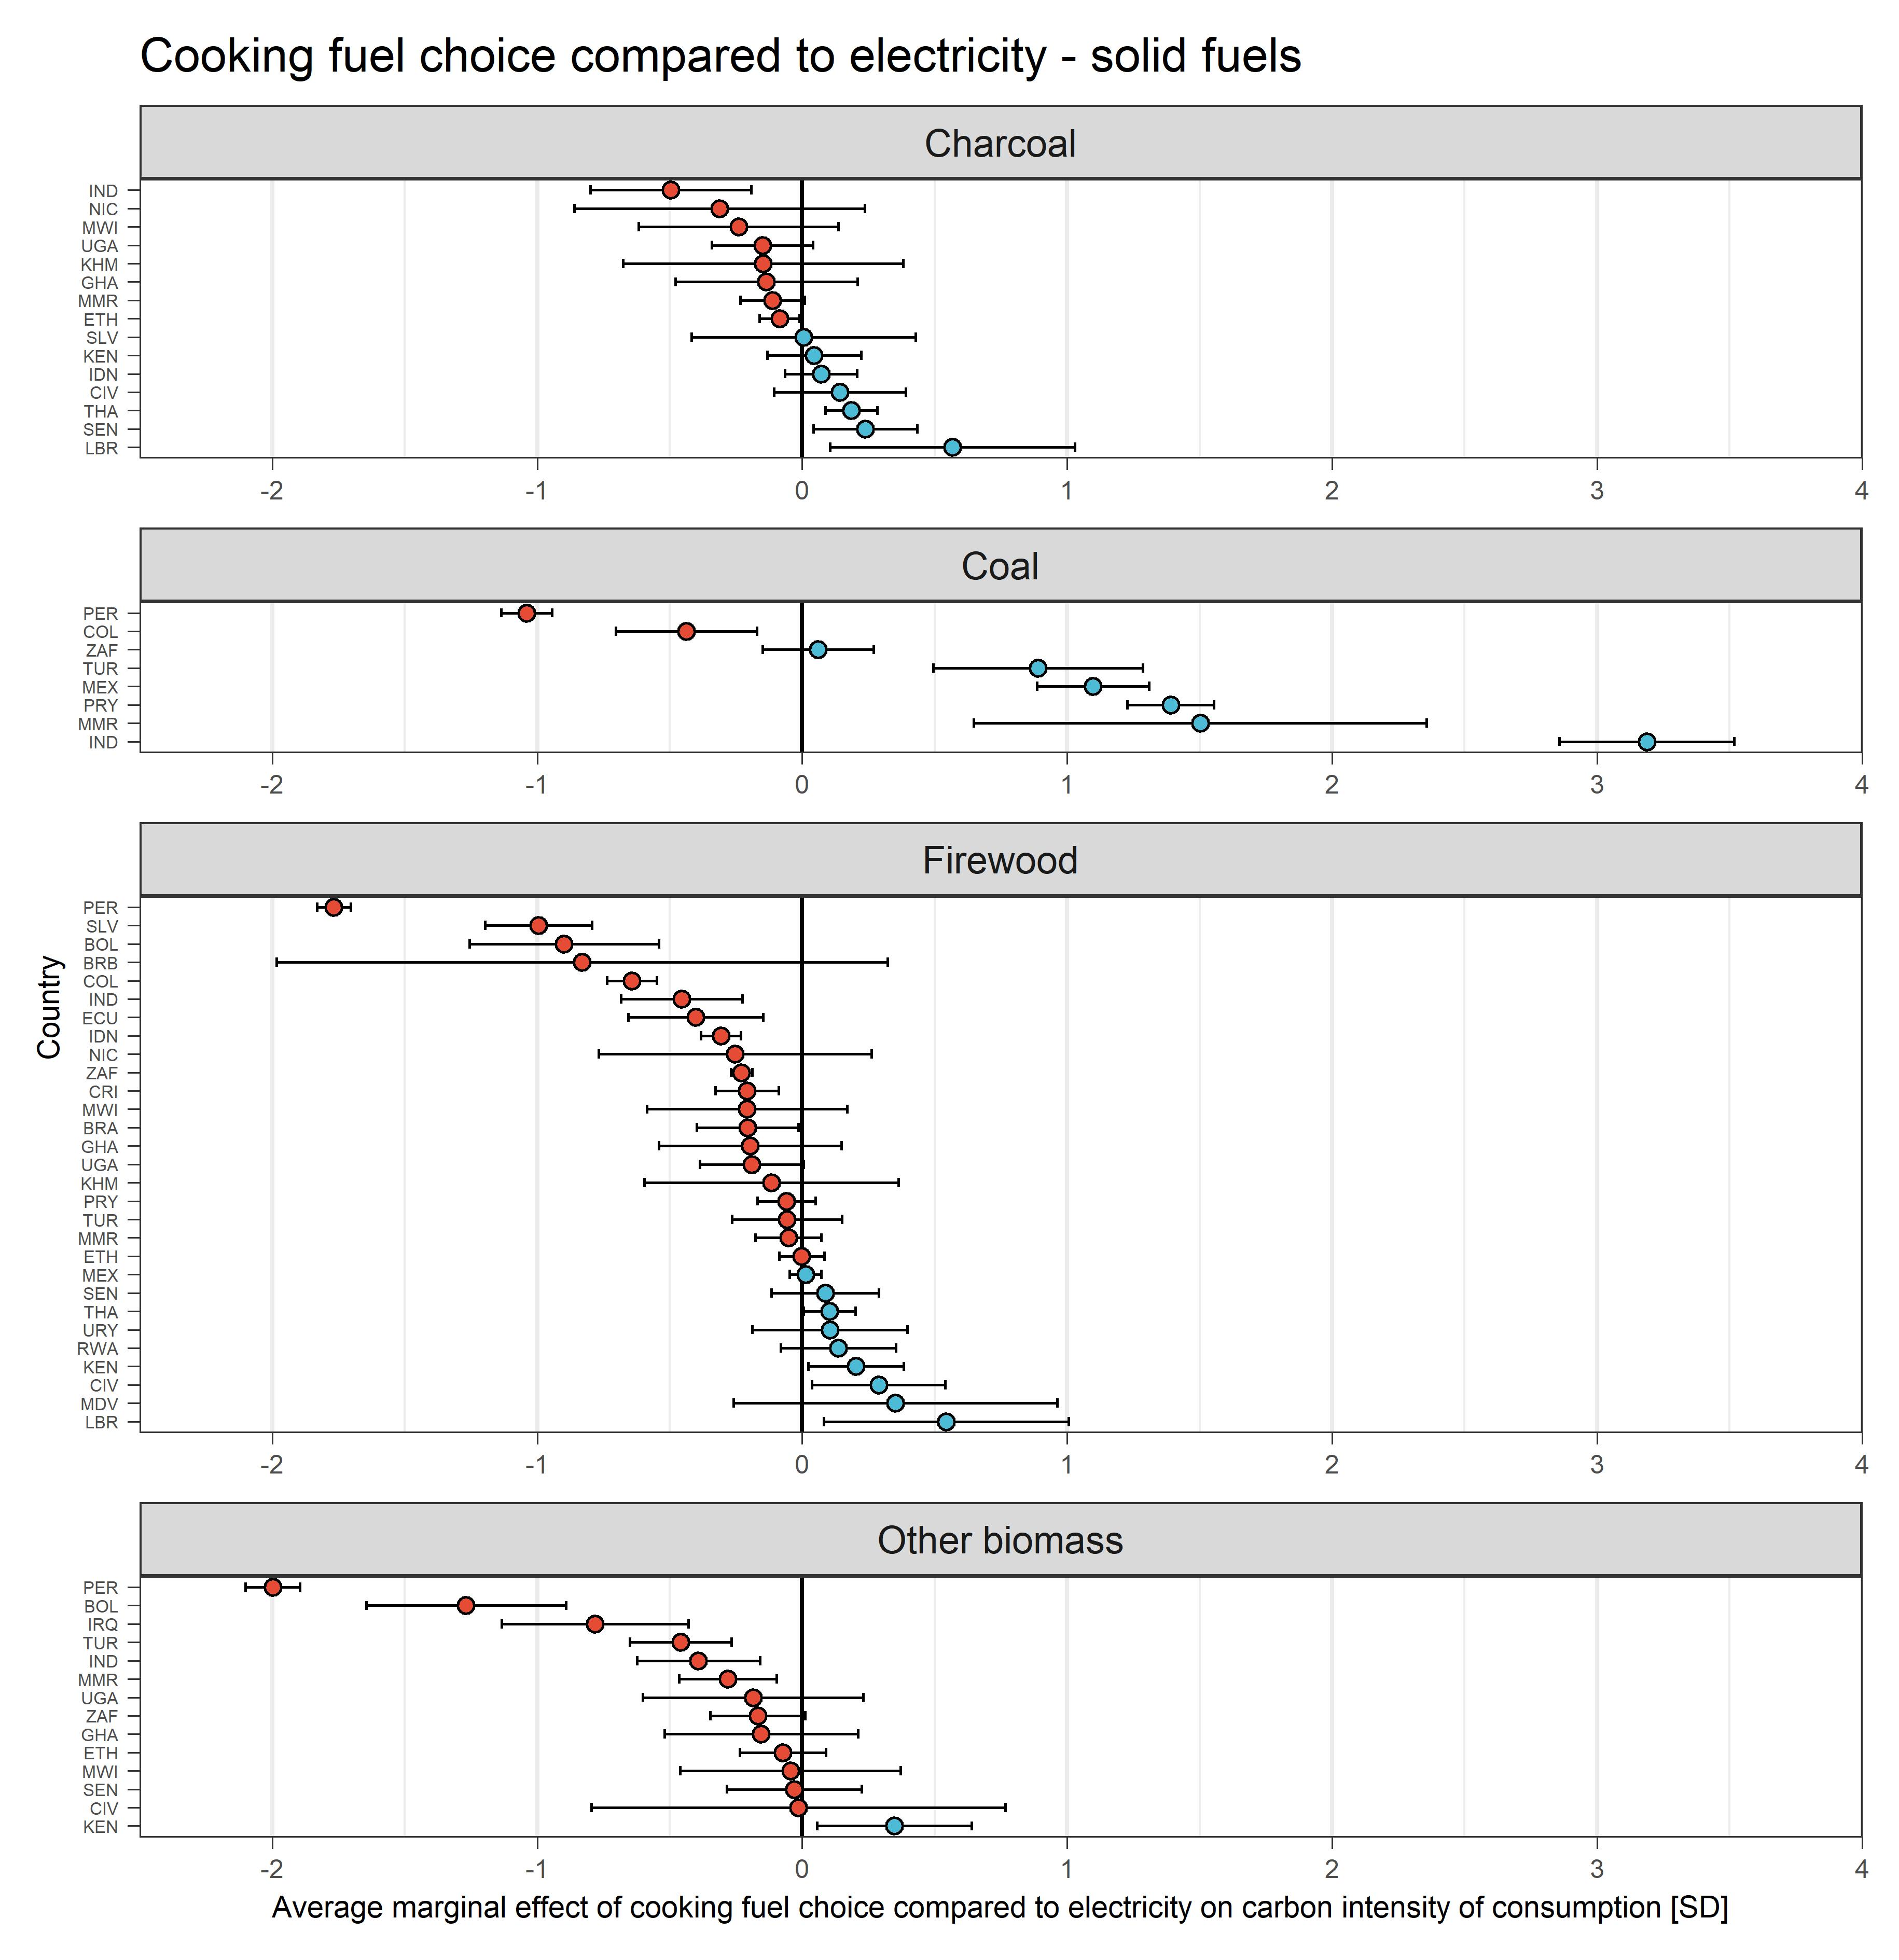
\includegraphics{Analysis_OLS_ME_Carbon_Intensity/AME_OLS_CI_CI_Electricity A}
%   %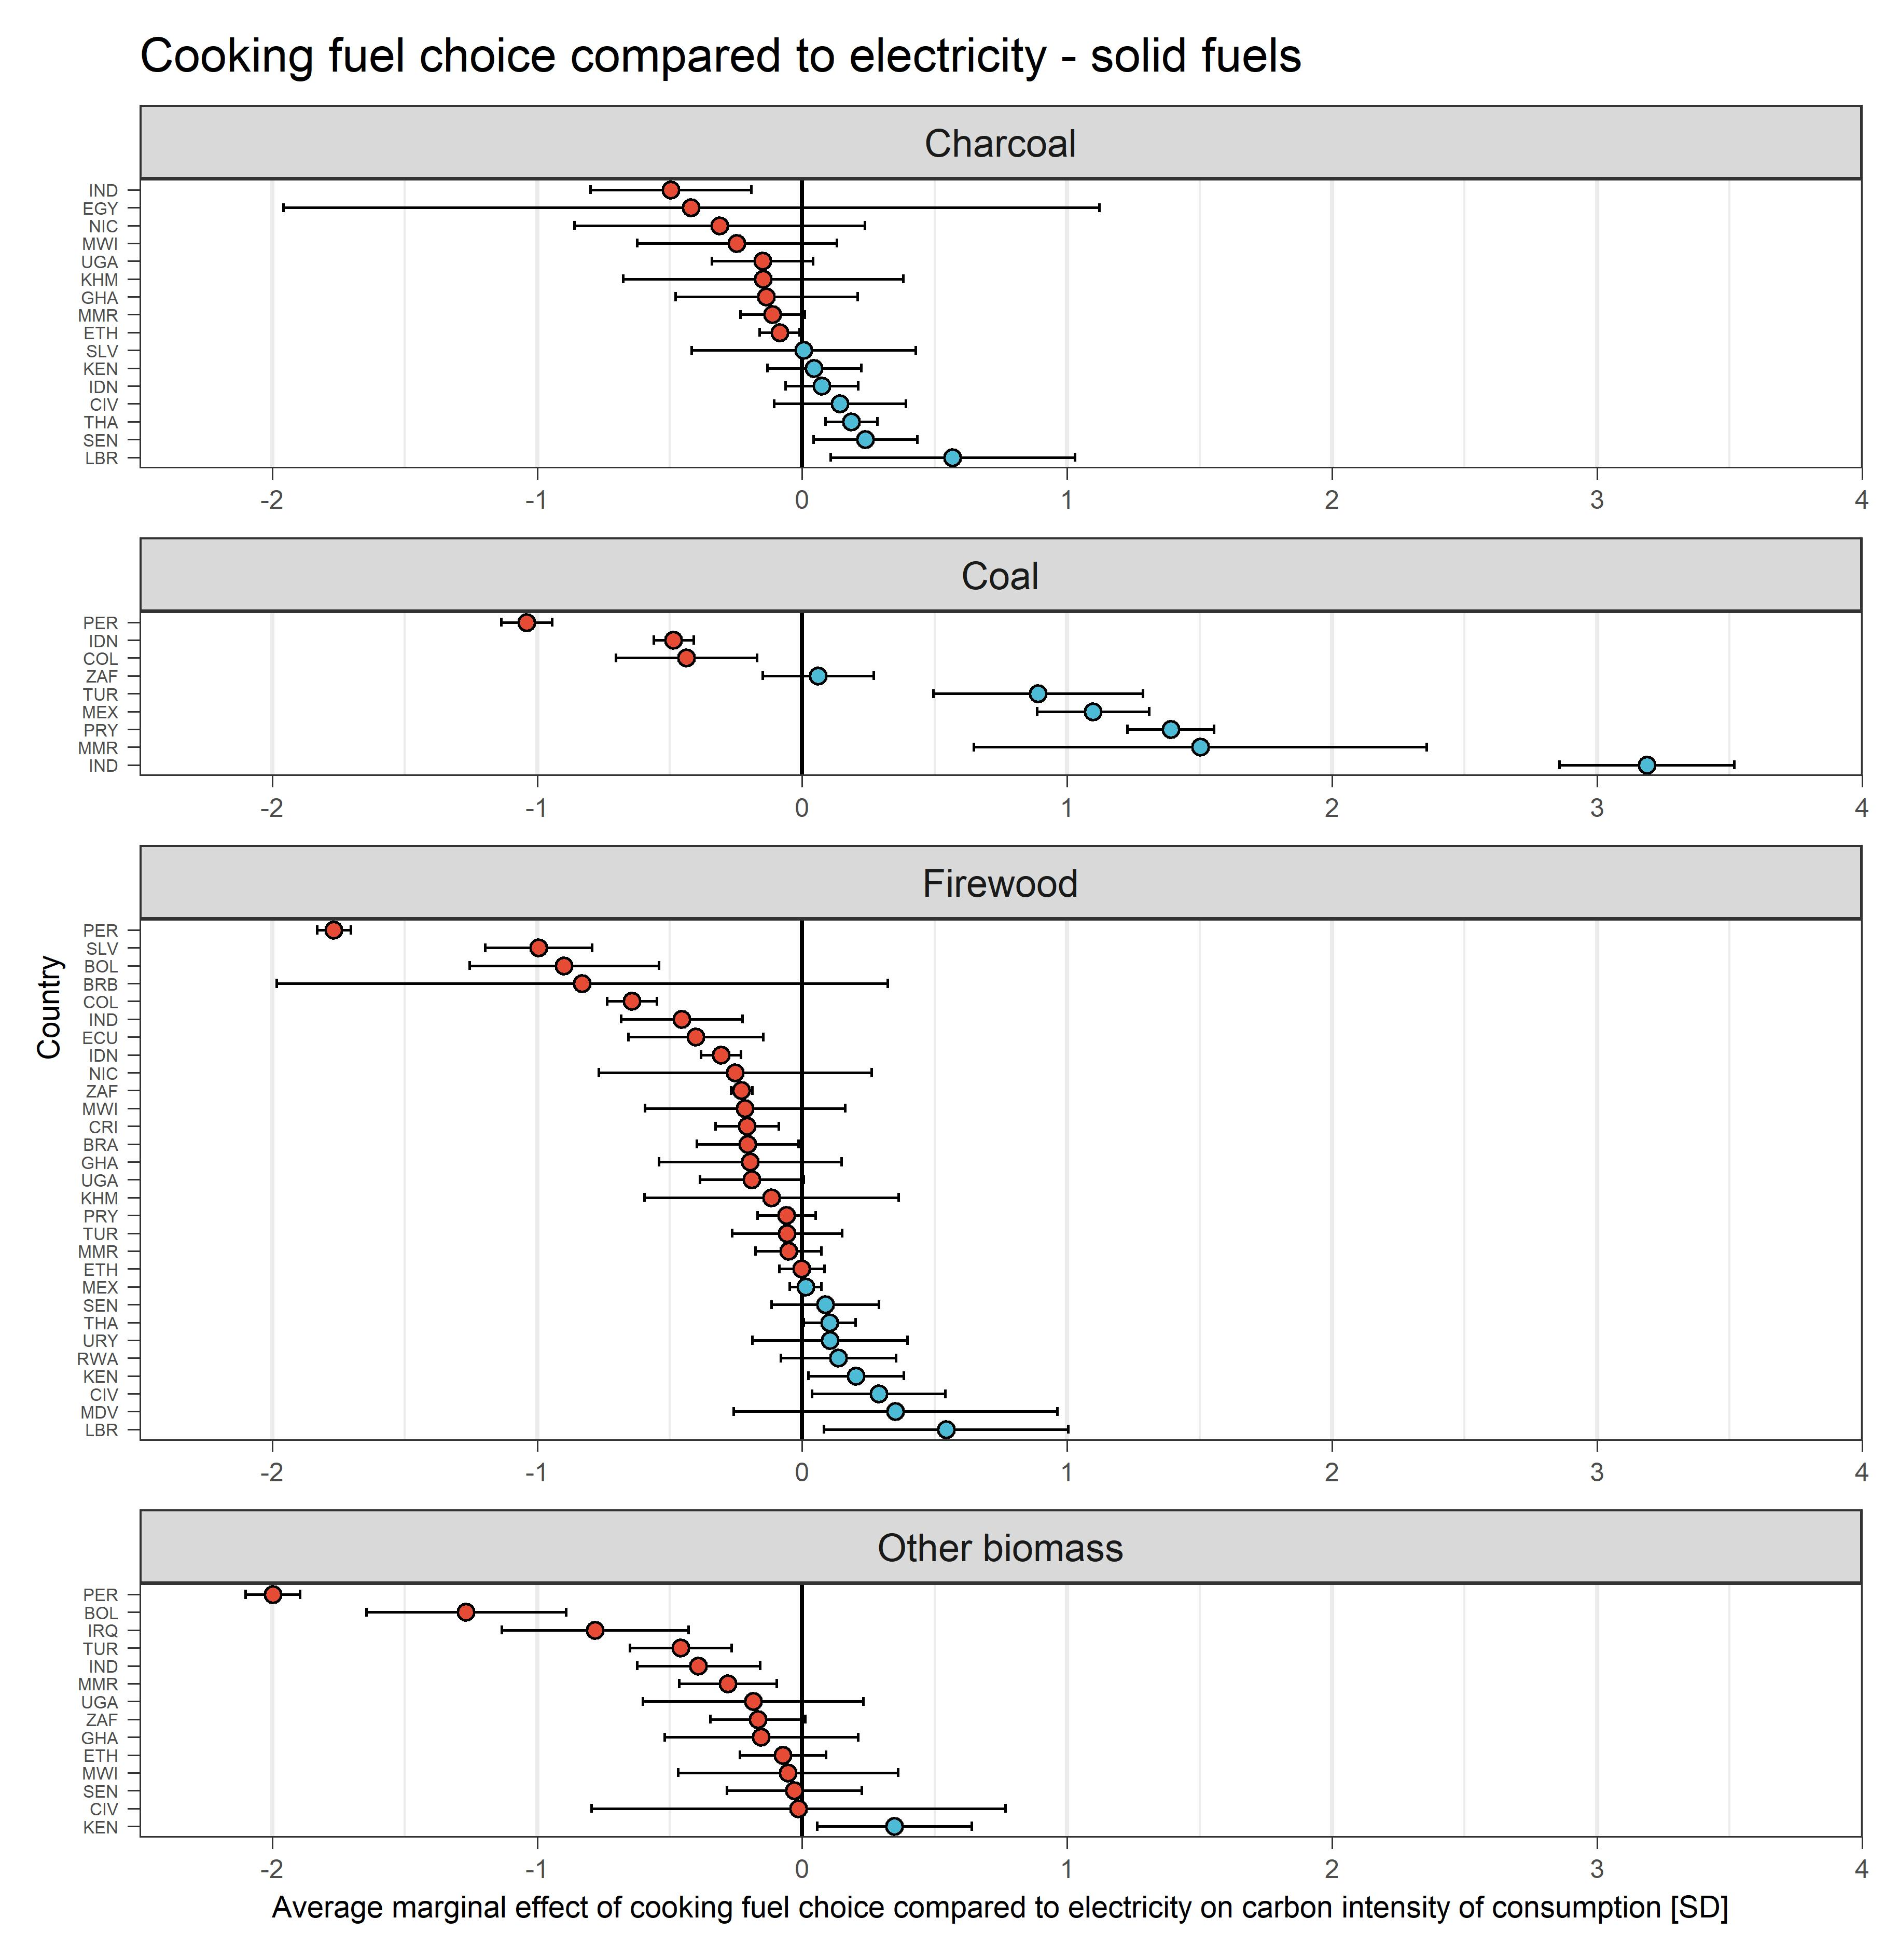
\includegraphics{Analysis_OLS_ME_Carbon_Intensity/AME_OLS_CI_CF_Electricity A}
%   \begin{subcaption}
%     This figure displays ...
%   \end{subcaption}

% \end{figure}

% \clearpage

% \begin{figure}[ht!]
%   \centering
%  \caption{Average marginal effects of cooking fuel choice - Part B} \label{fig:E7_Electricity_B}
%   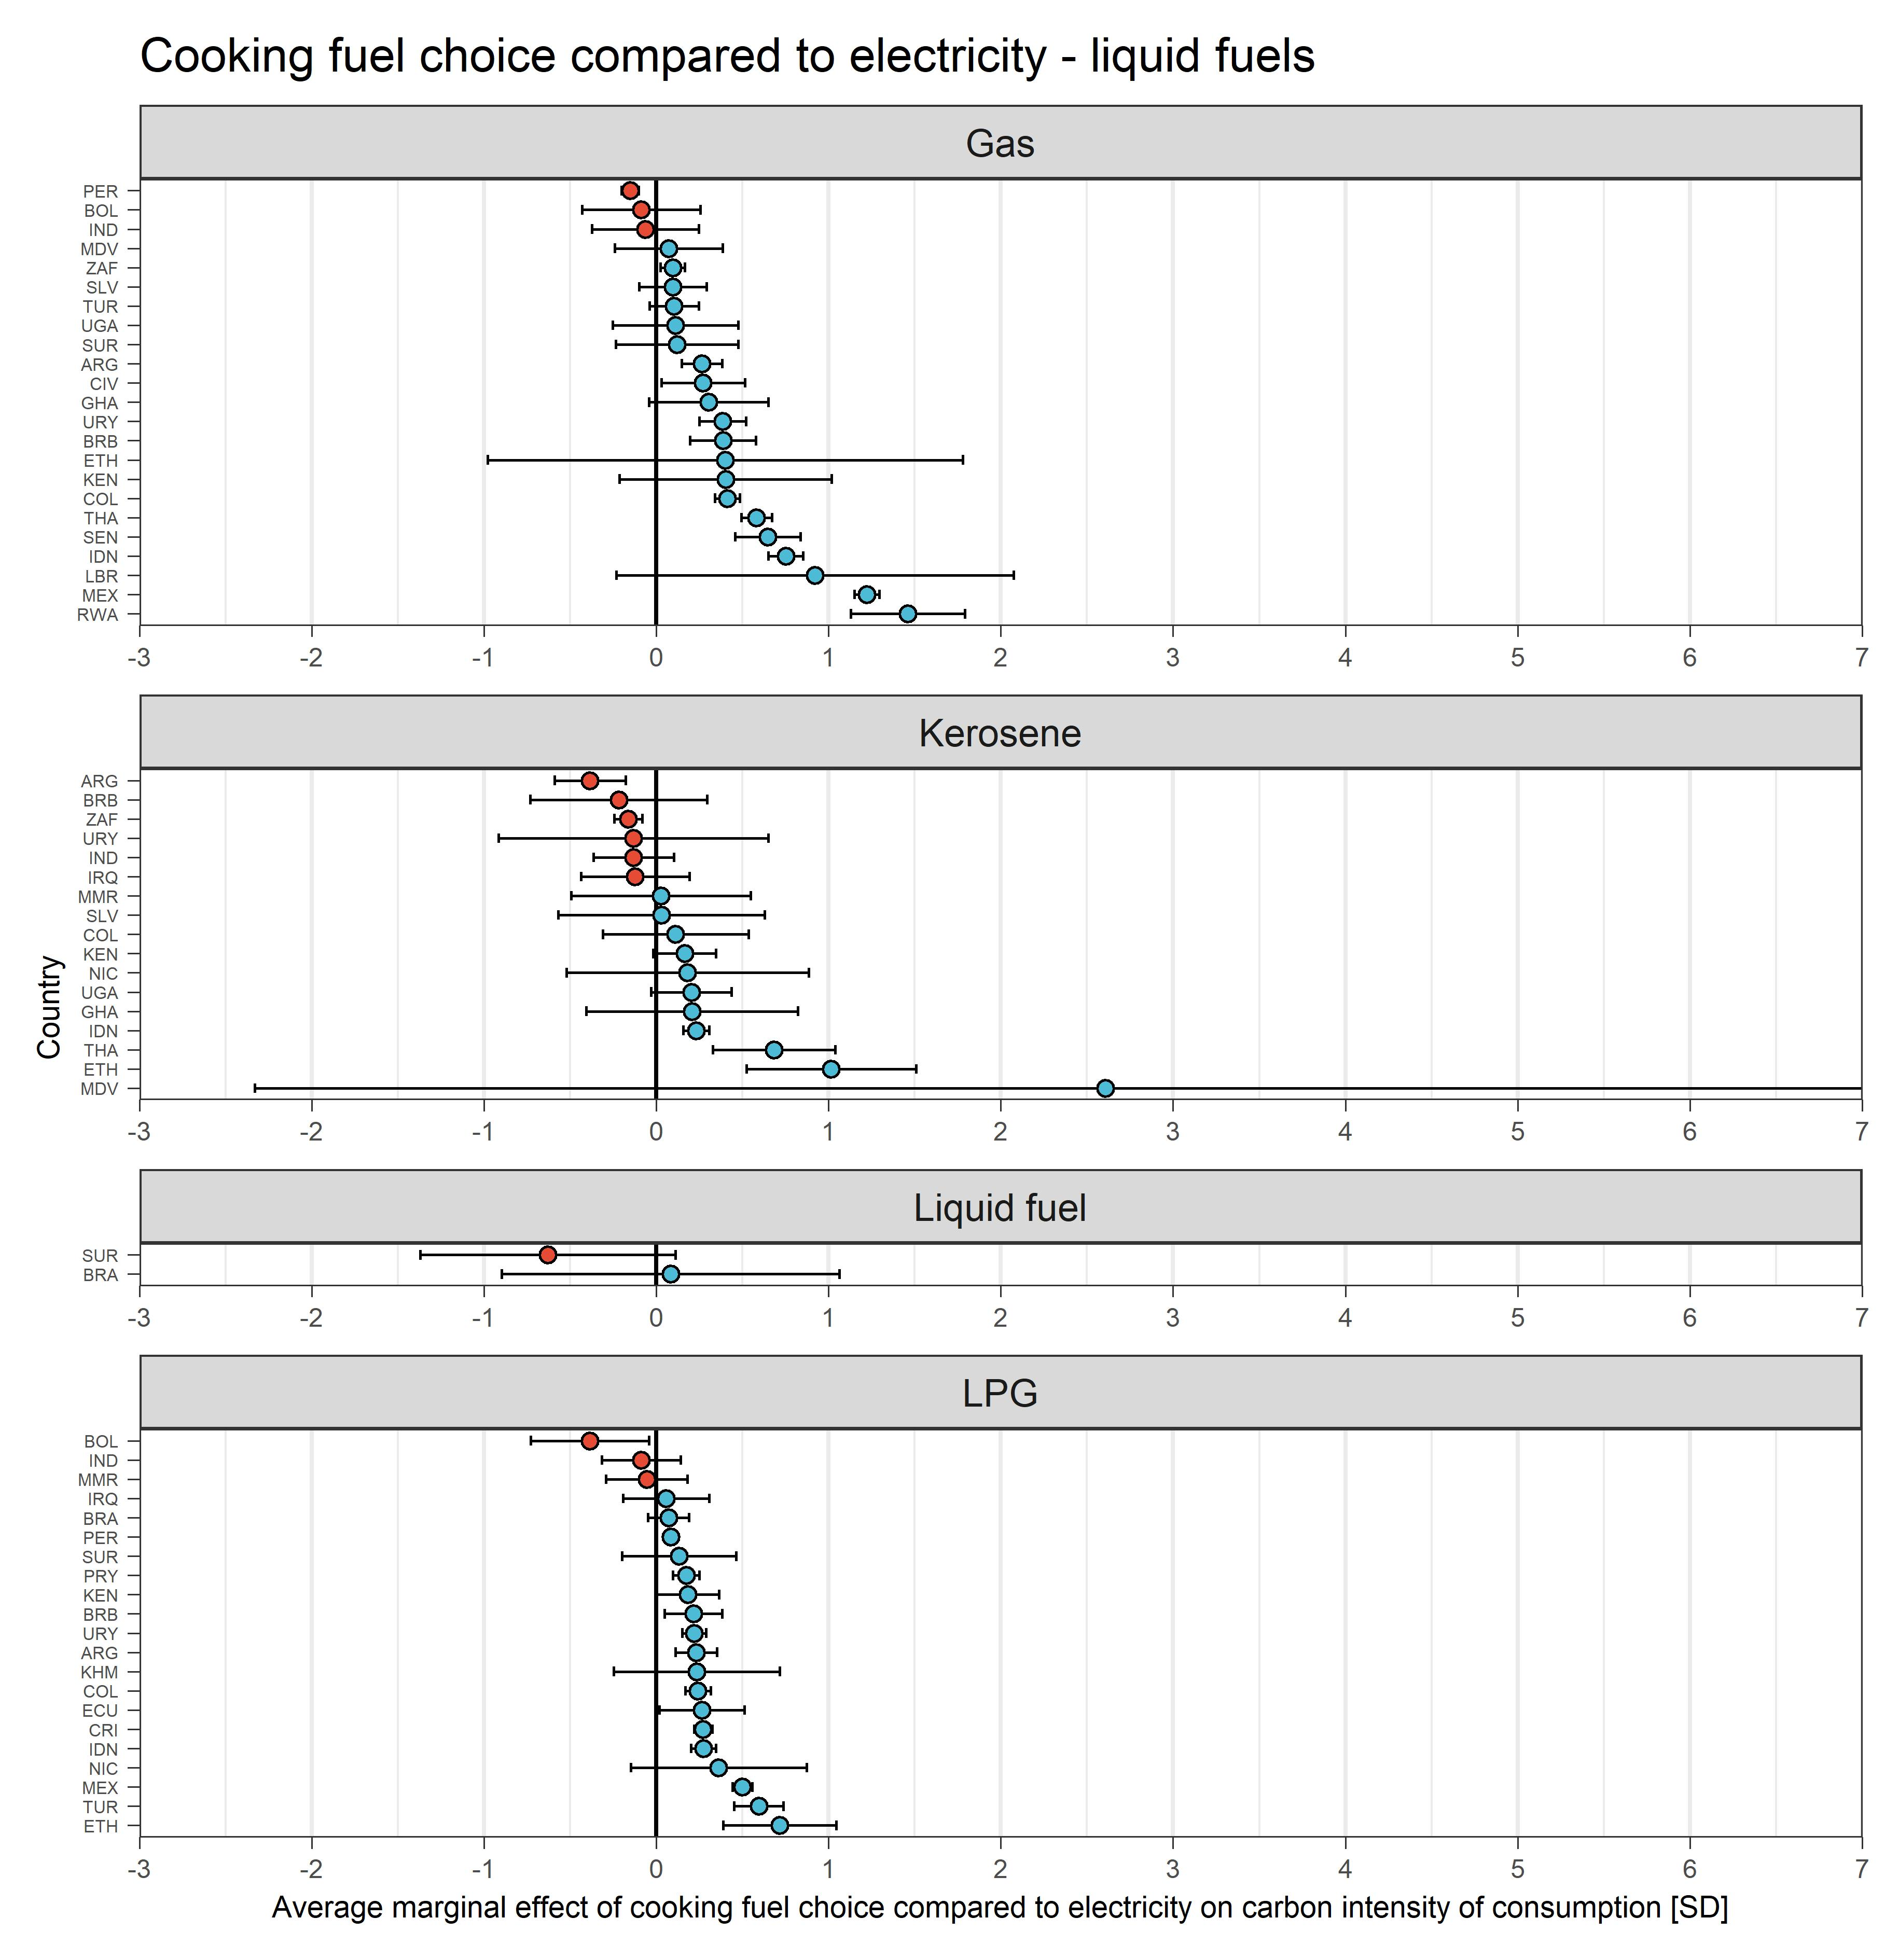
\includegraphics{Analysis_OLS_ME_Carbon_Intensity/AME_OLS_CI_CI_Electricity B}
%   %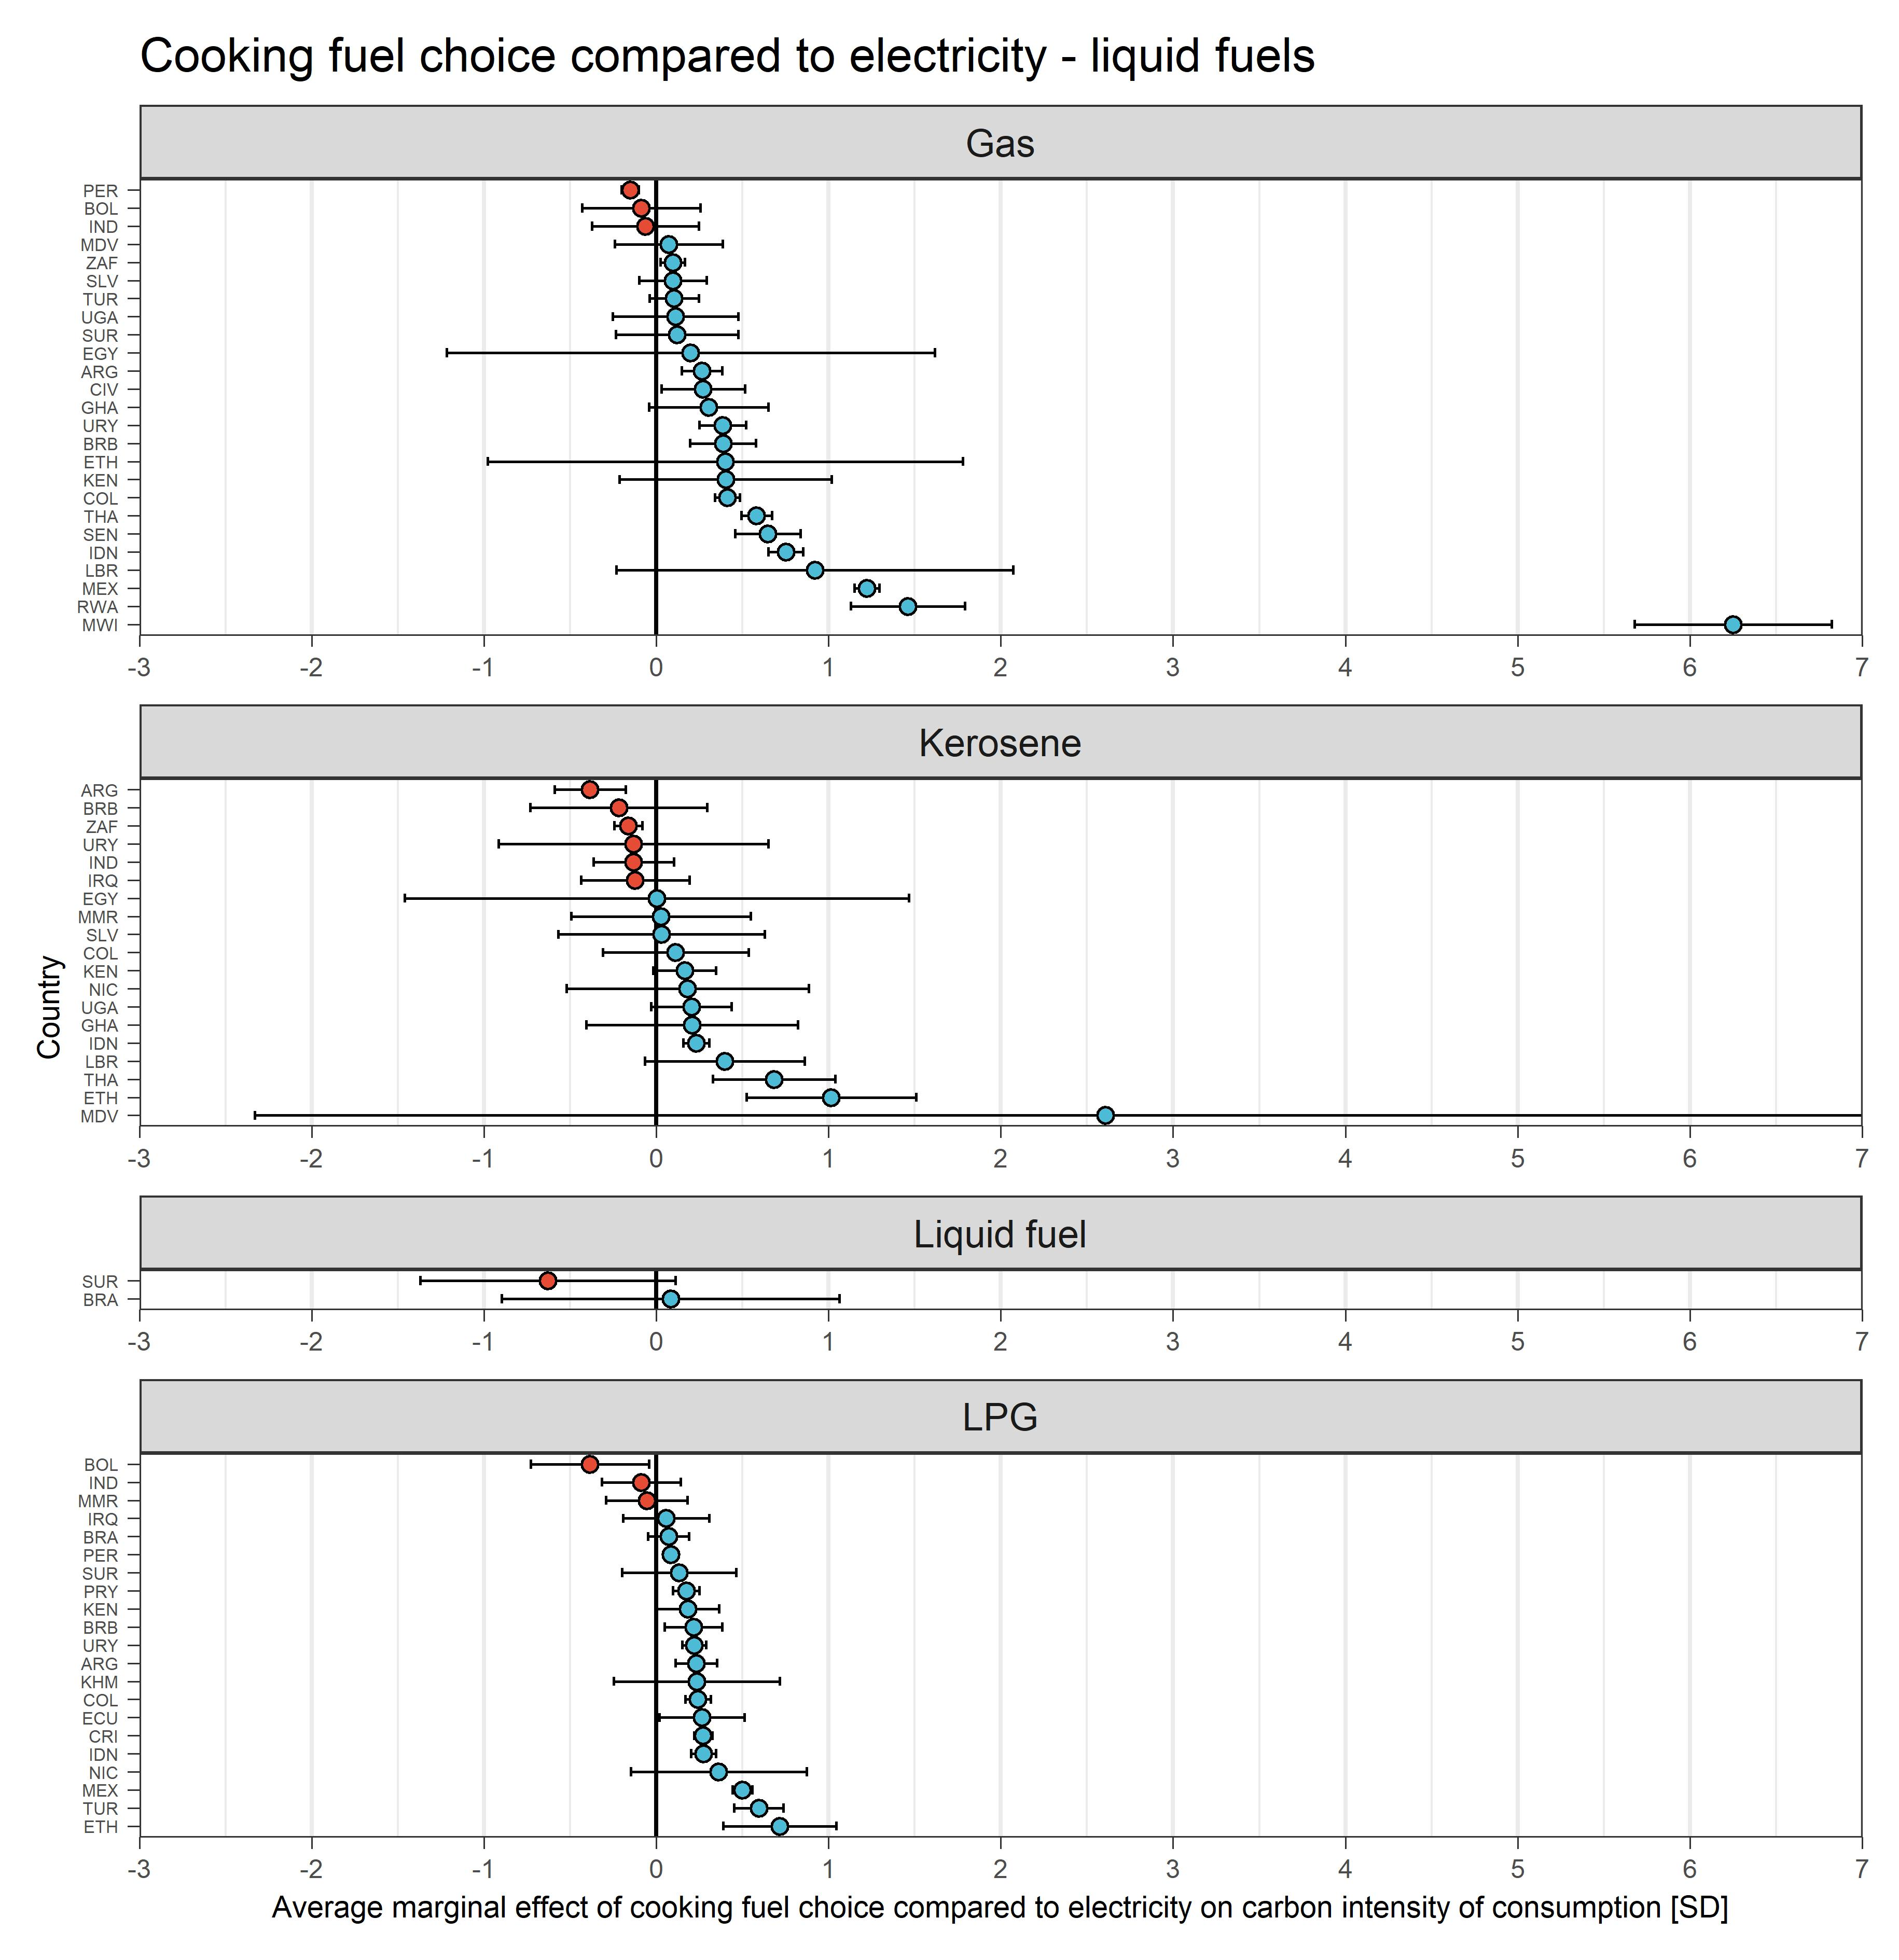
\includegraphics{Analysis_OLS_ME_Carbon_Intensity/AME_OLS_CI_CF_Electricity B}
%   \begin{subcaption}
%     This figure displays ...
%   \end{subcaption}

% \end{figure}

% \clearpage

% \begin{figure}[ht!]
%   \centering
%  \caption{Average marginal effects of cooking fuel choice - Part C} \label{fig:E8_LPG}
%   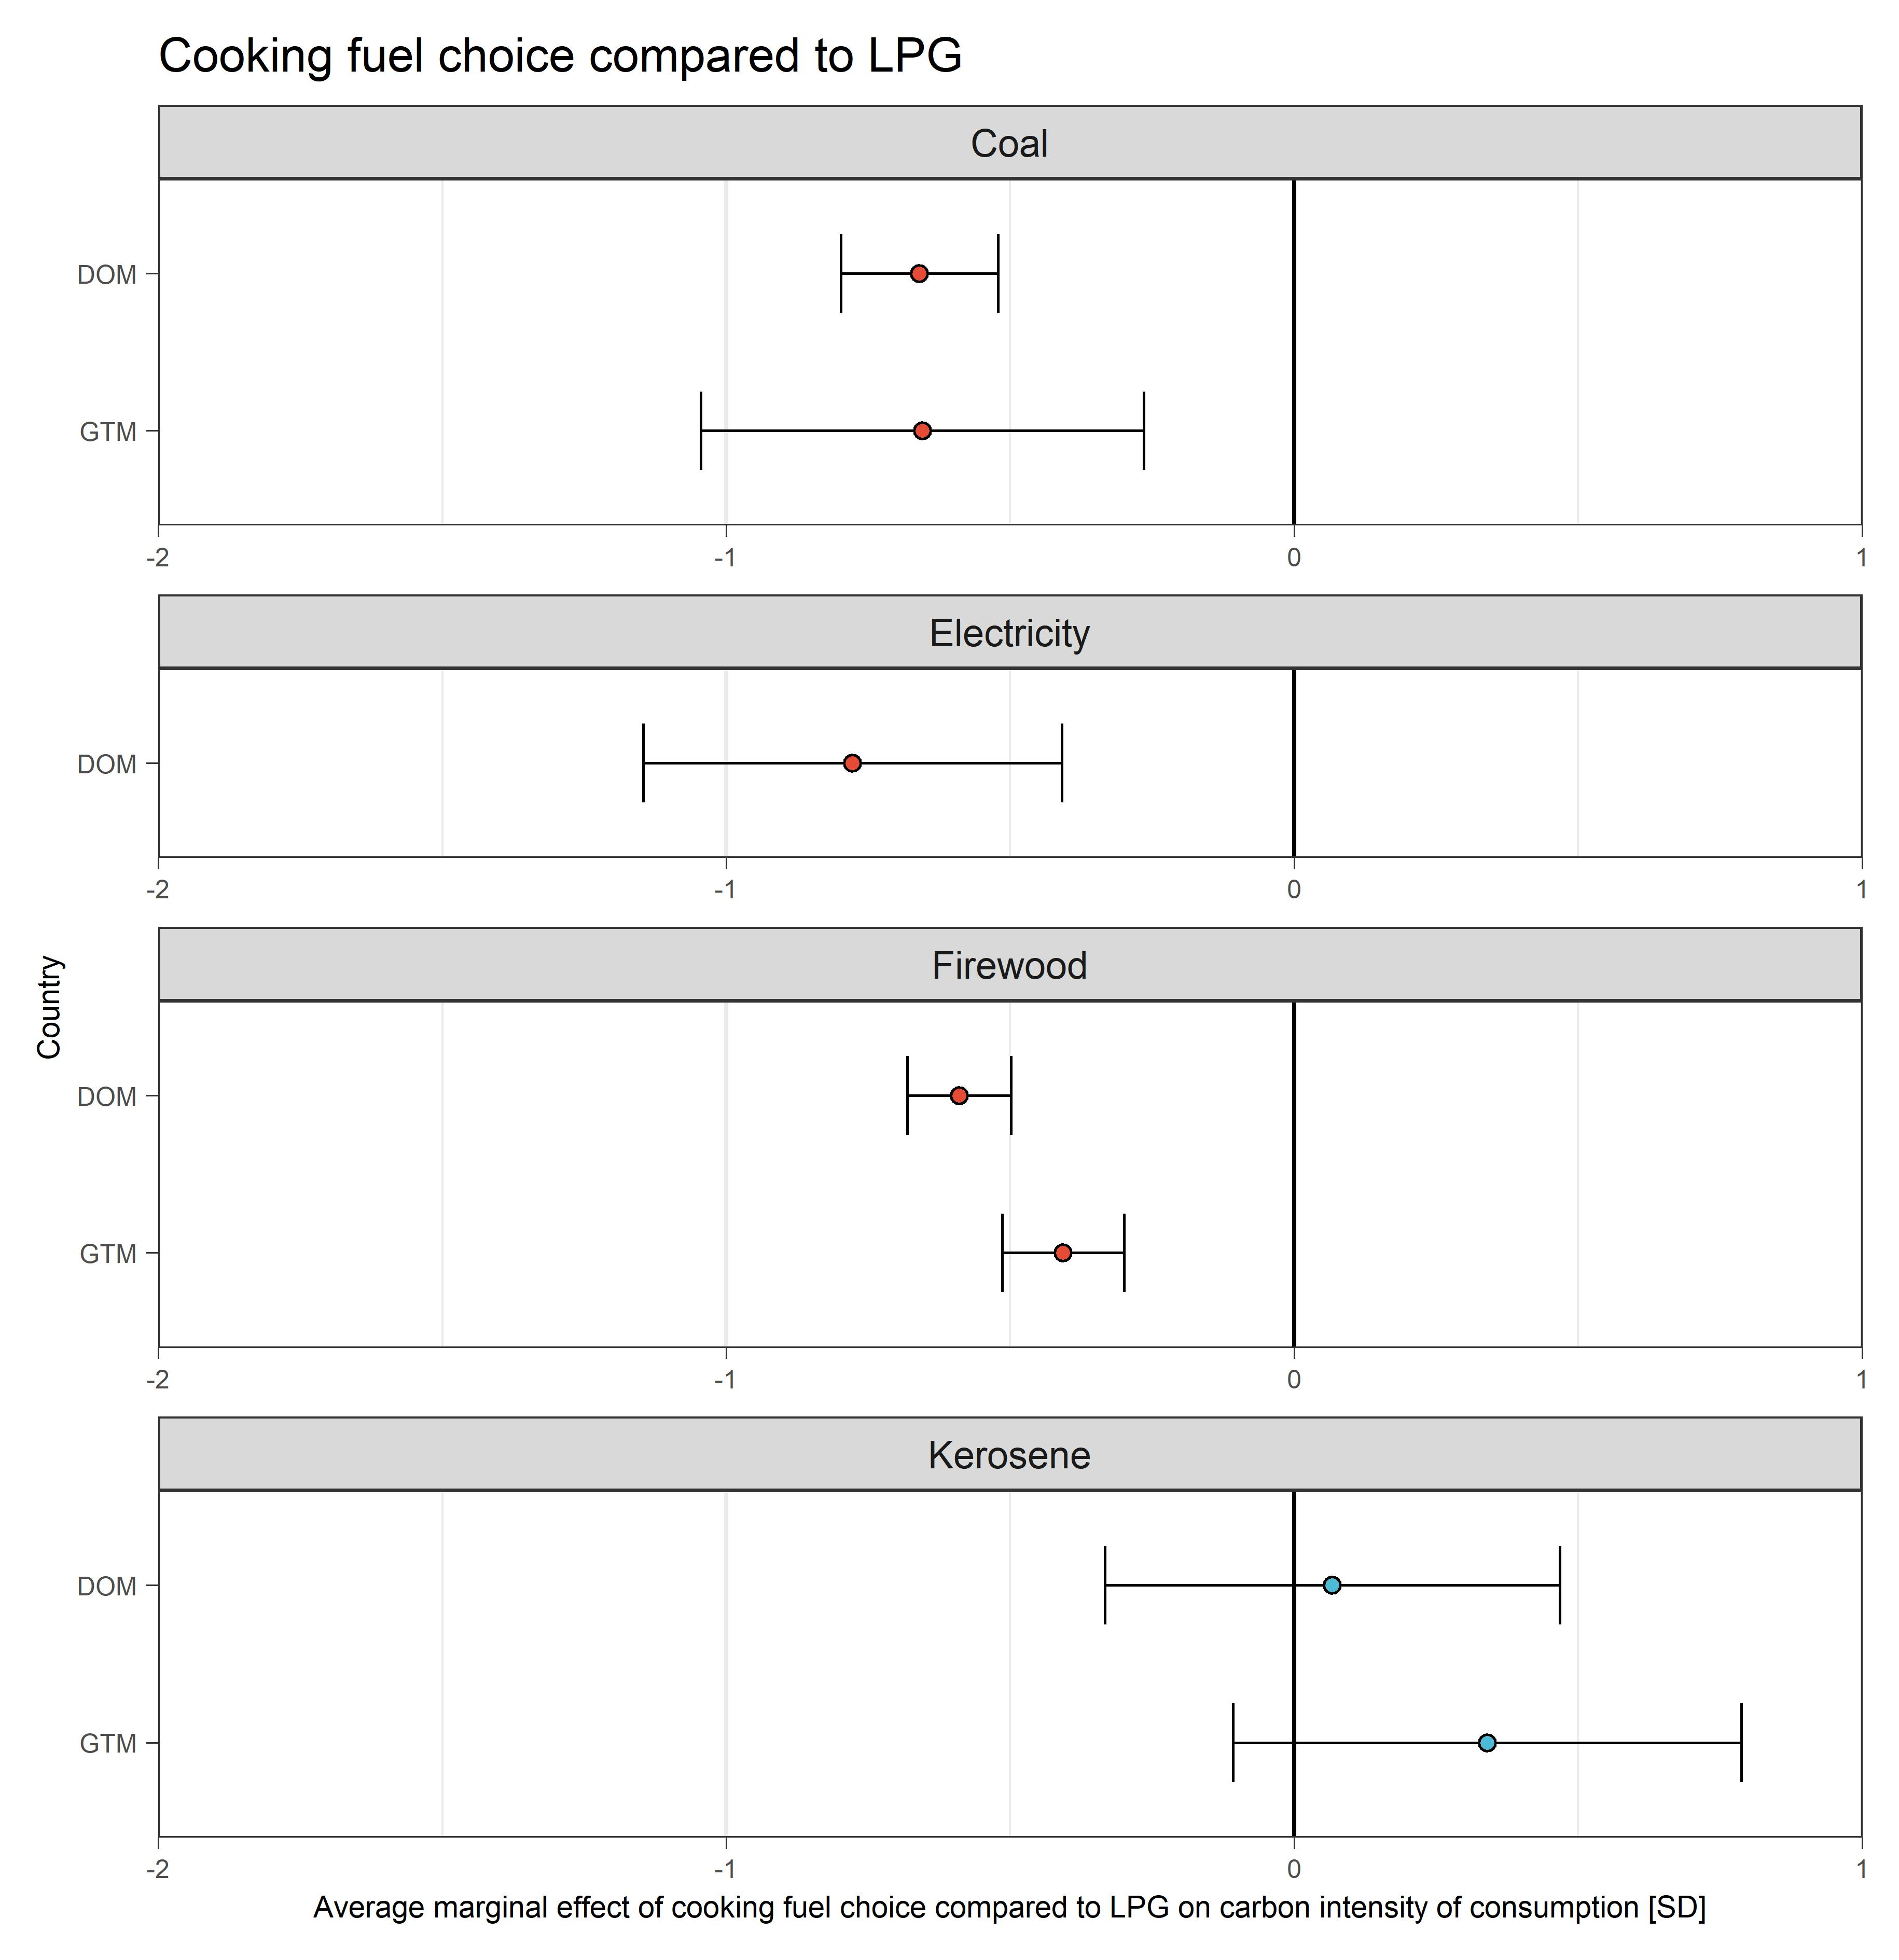
\includegraphics{Analysis_OLS_ME_Carbon_Intensity/AME_OLS_CI_CI_LPG}
%   %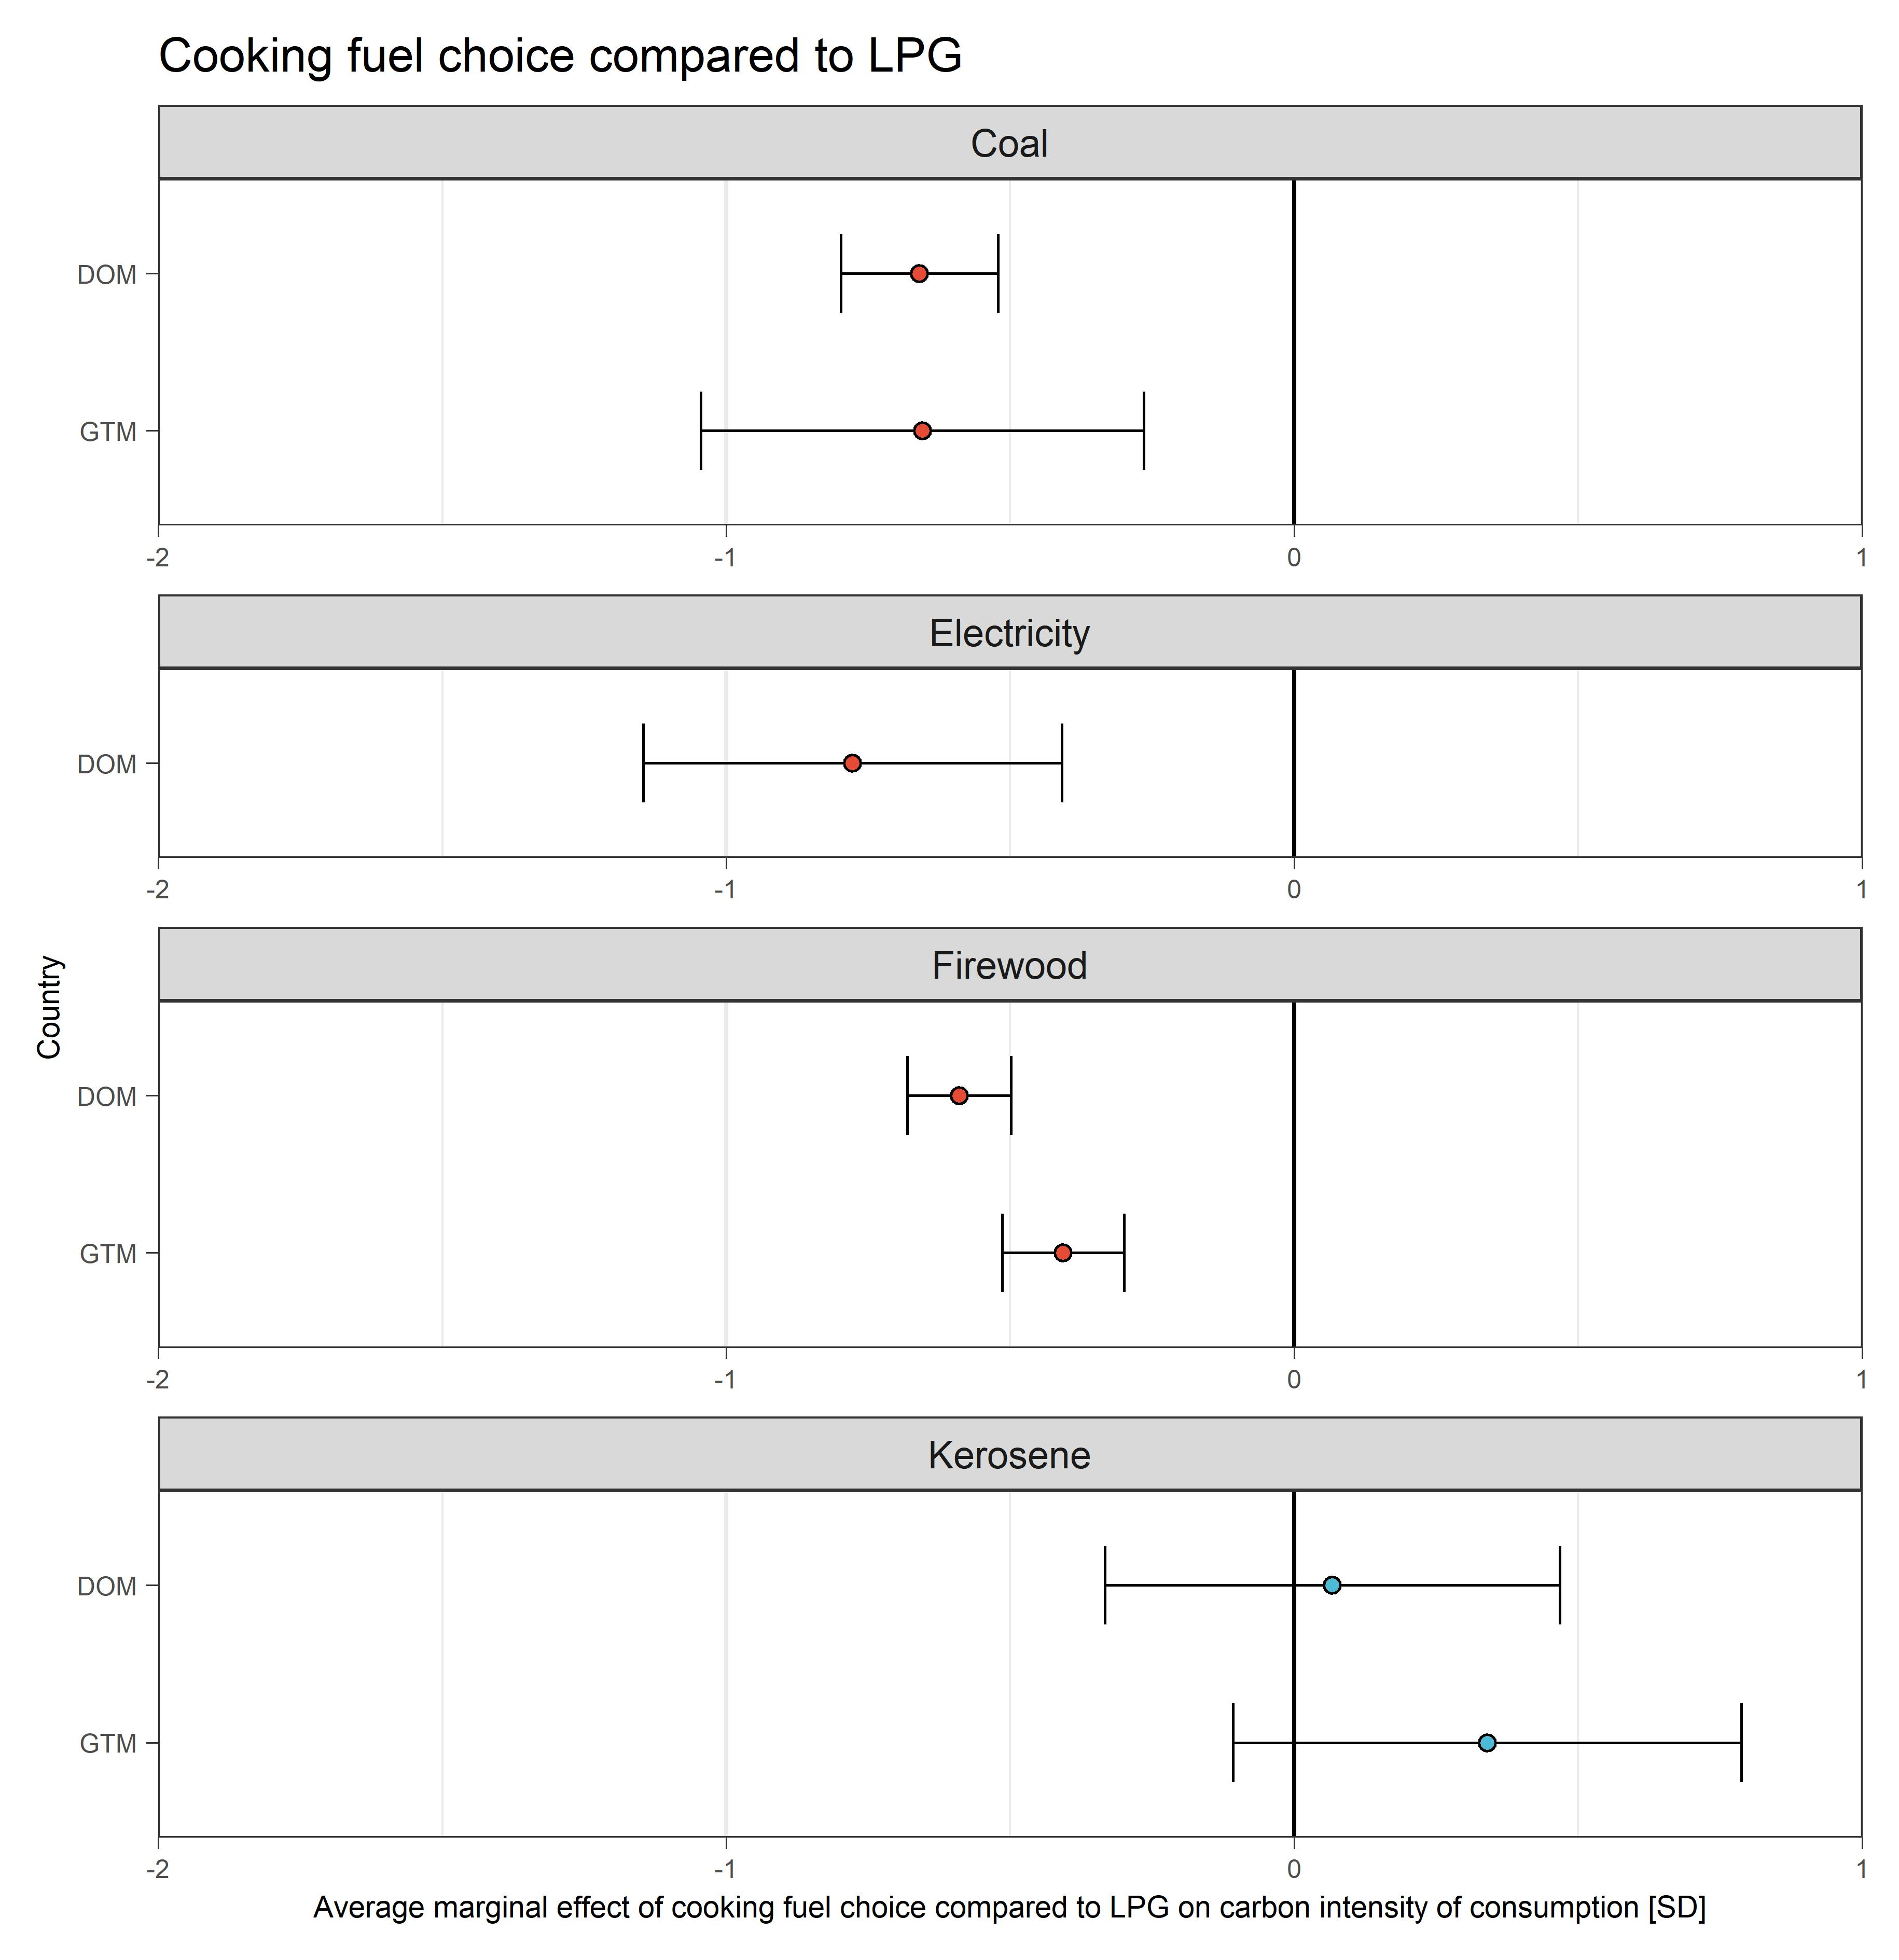
\includegraphics{Analysis_OLS_ME_Carbon_Intensity/AME_OLS_CI_CF_LPG}
%   \begin{subcaption}
%     This figure displays ...
%   \end{subcaption}

% \end{figure}

% \clearpage

% \begin{figure}[ht!]
%   \centering
%  \caption{Average marginal effects of cooking fuel choice - Part D} \label{fig:E9_Charcoal}
%   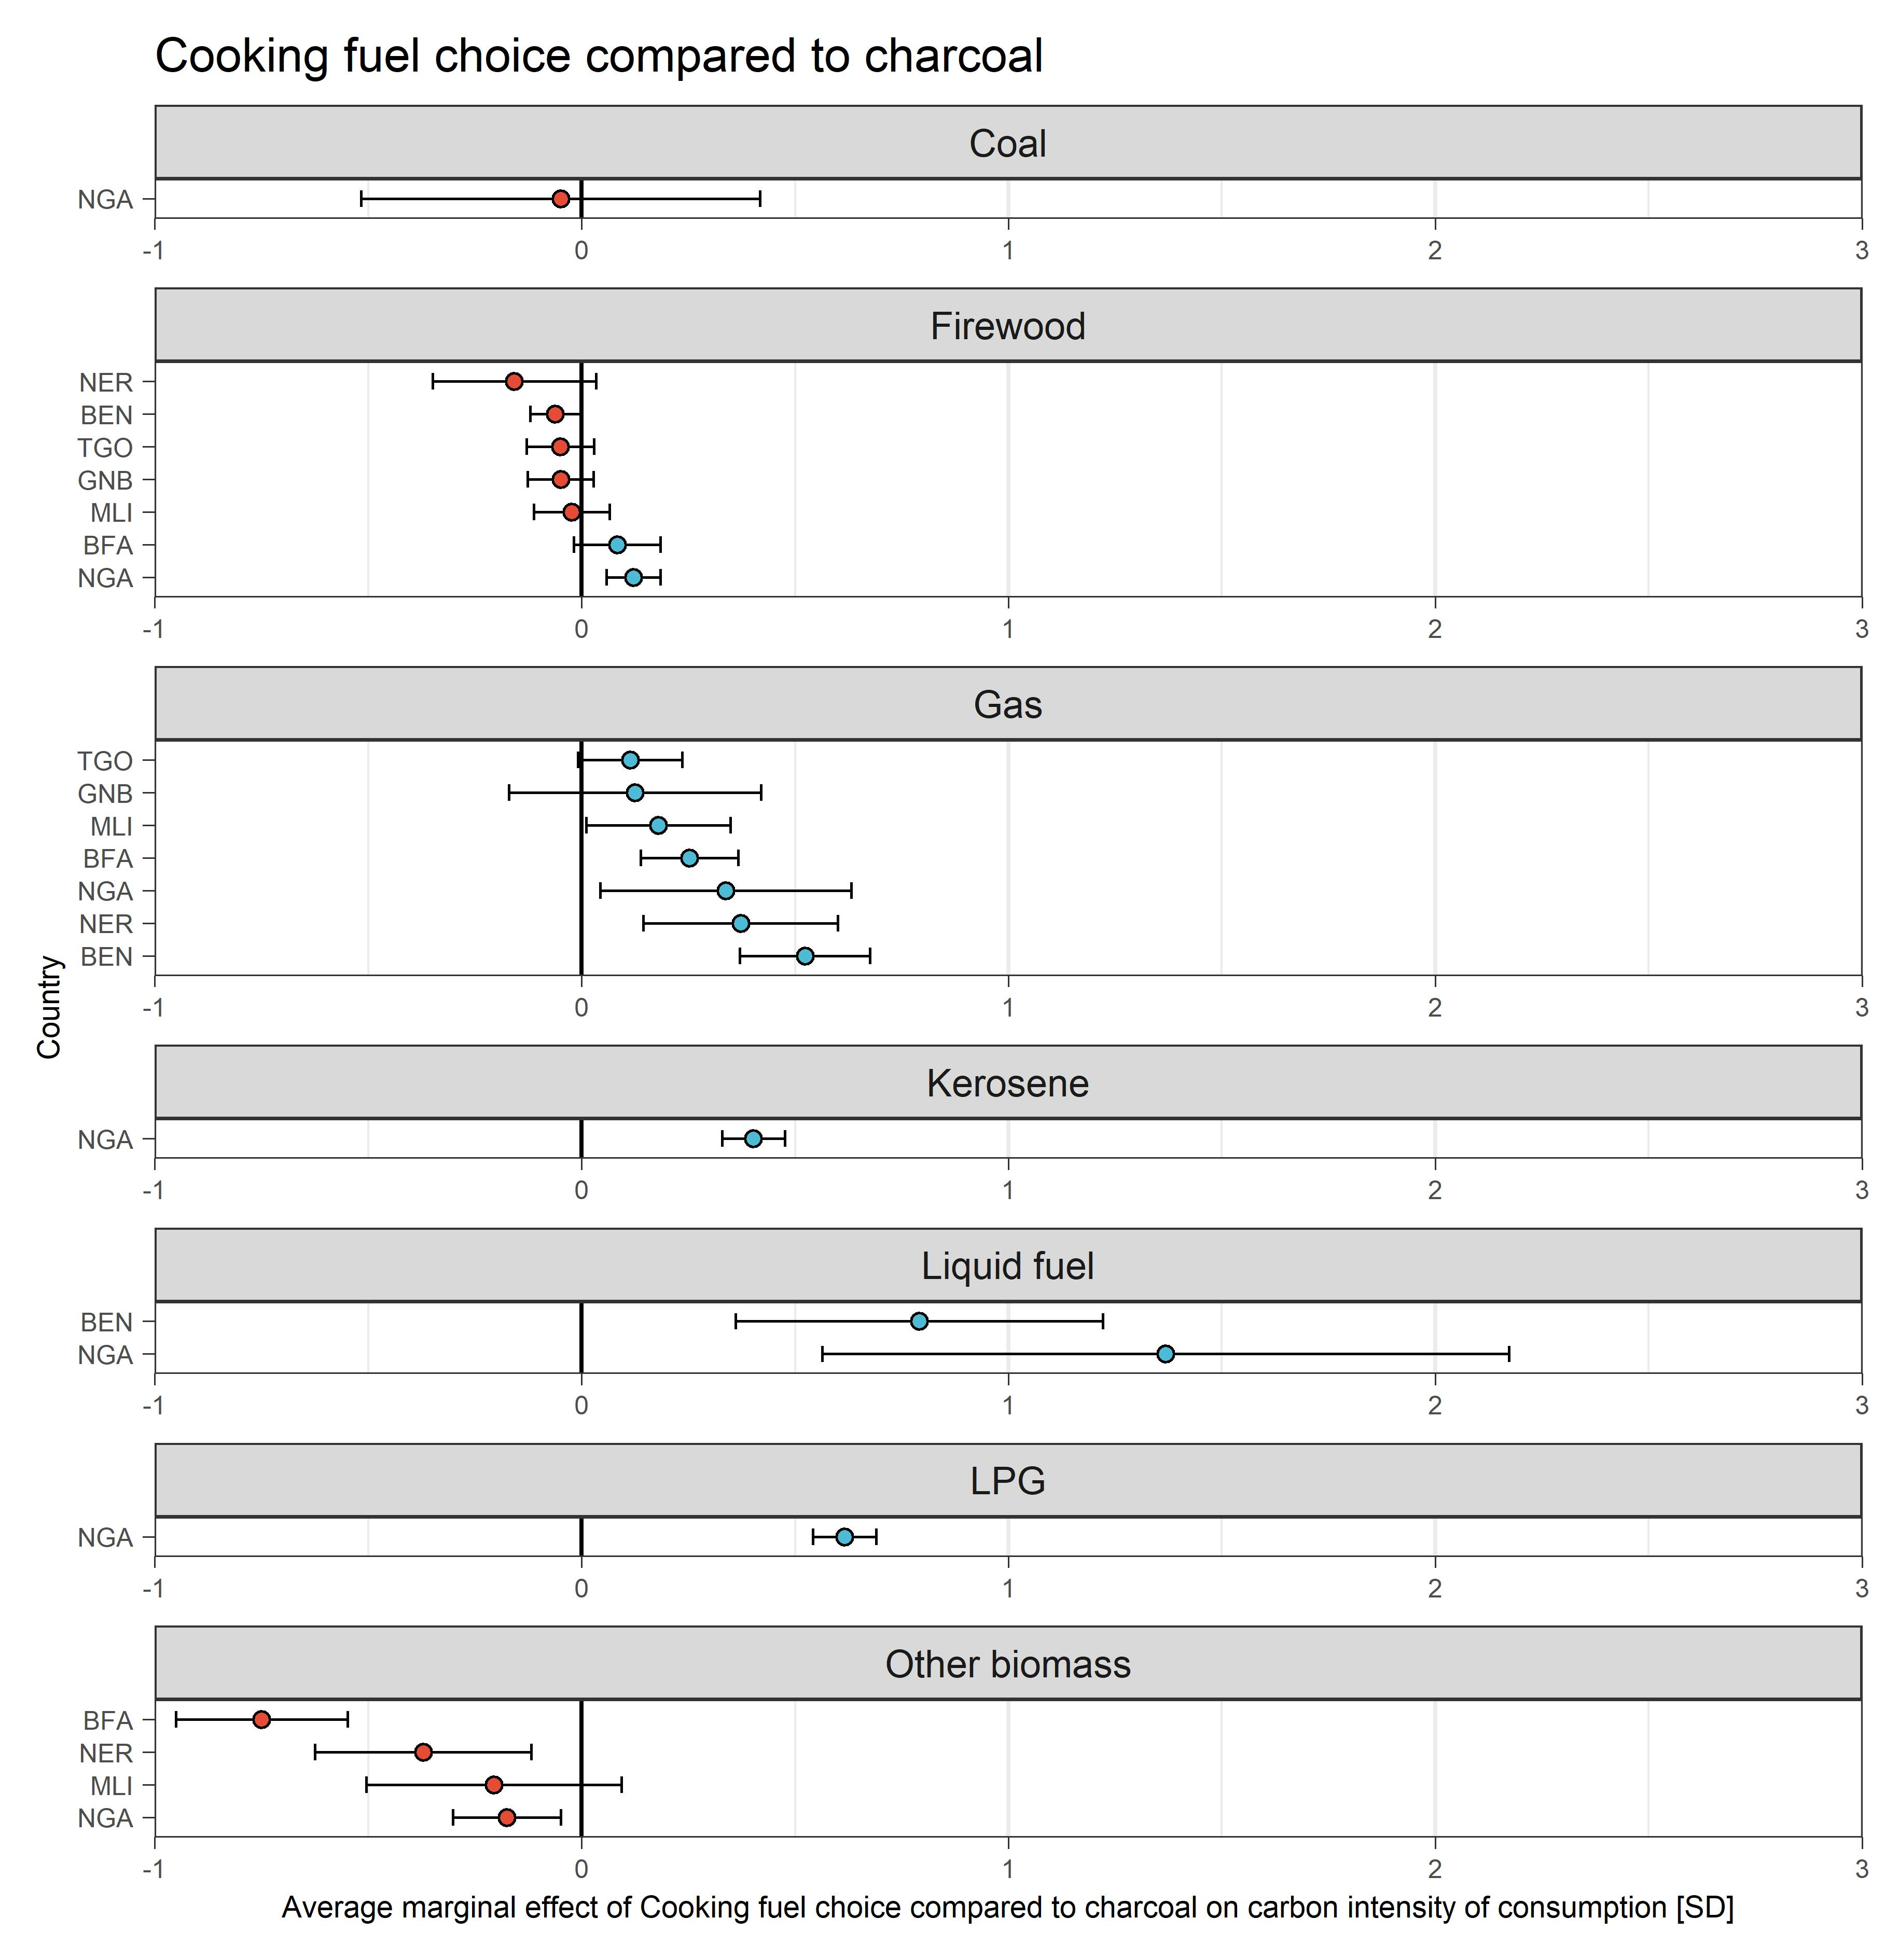
\includegraphics{Analysis_OLS_ME_Carbon_Intensity/AME_OLS_CI_CI_Charcoal}
%   %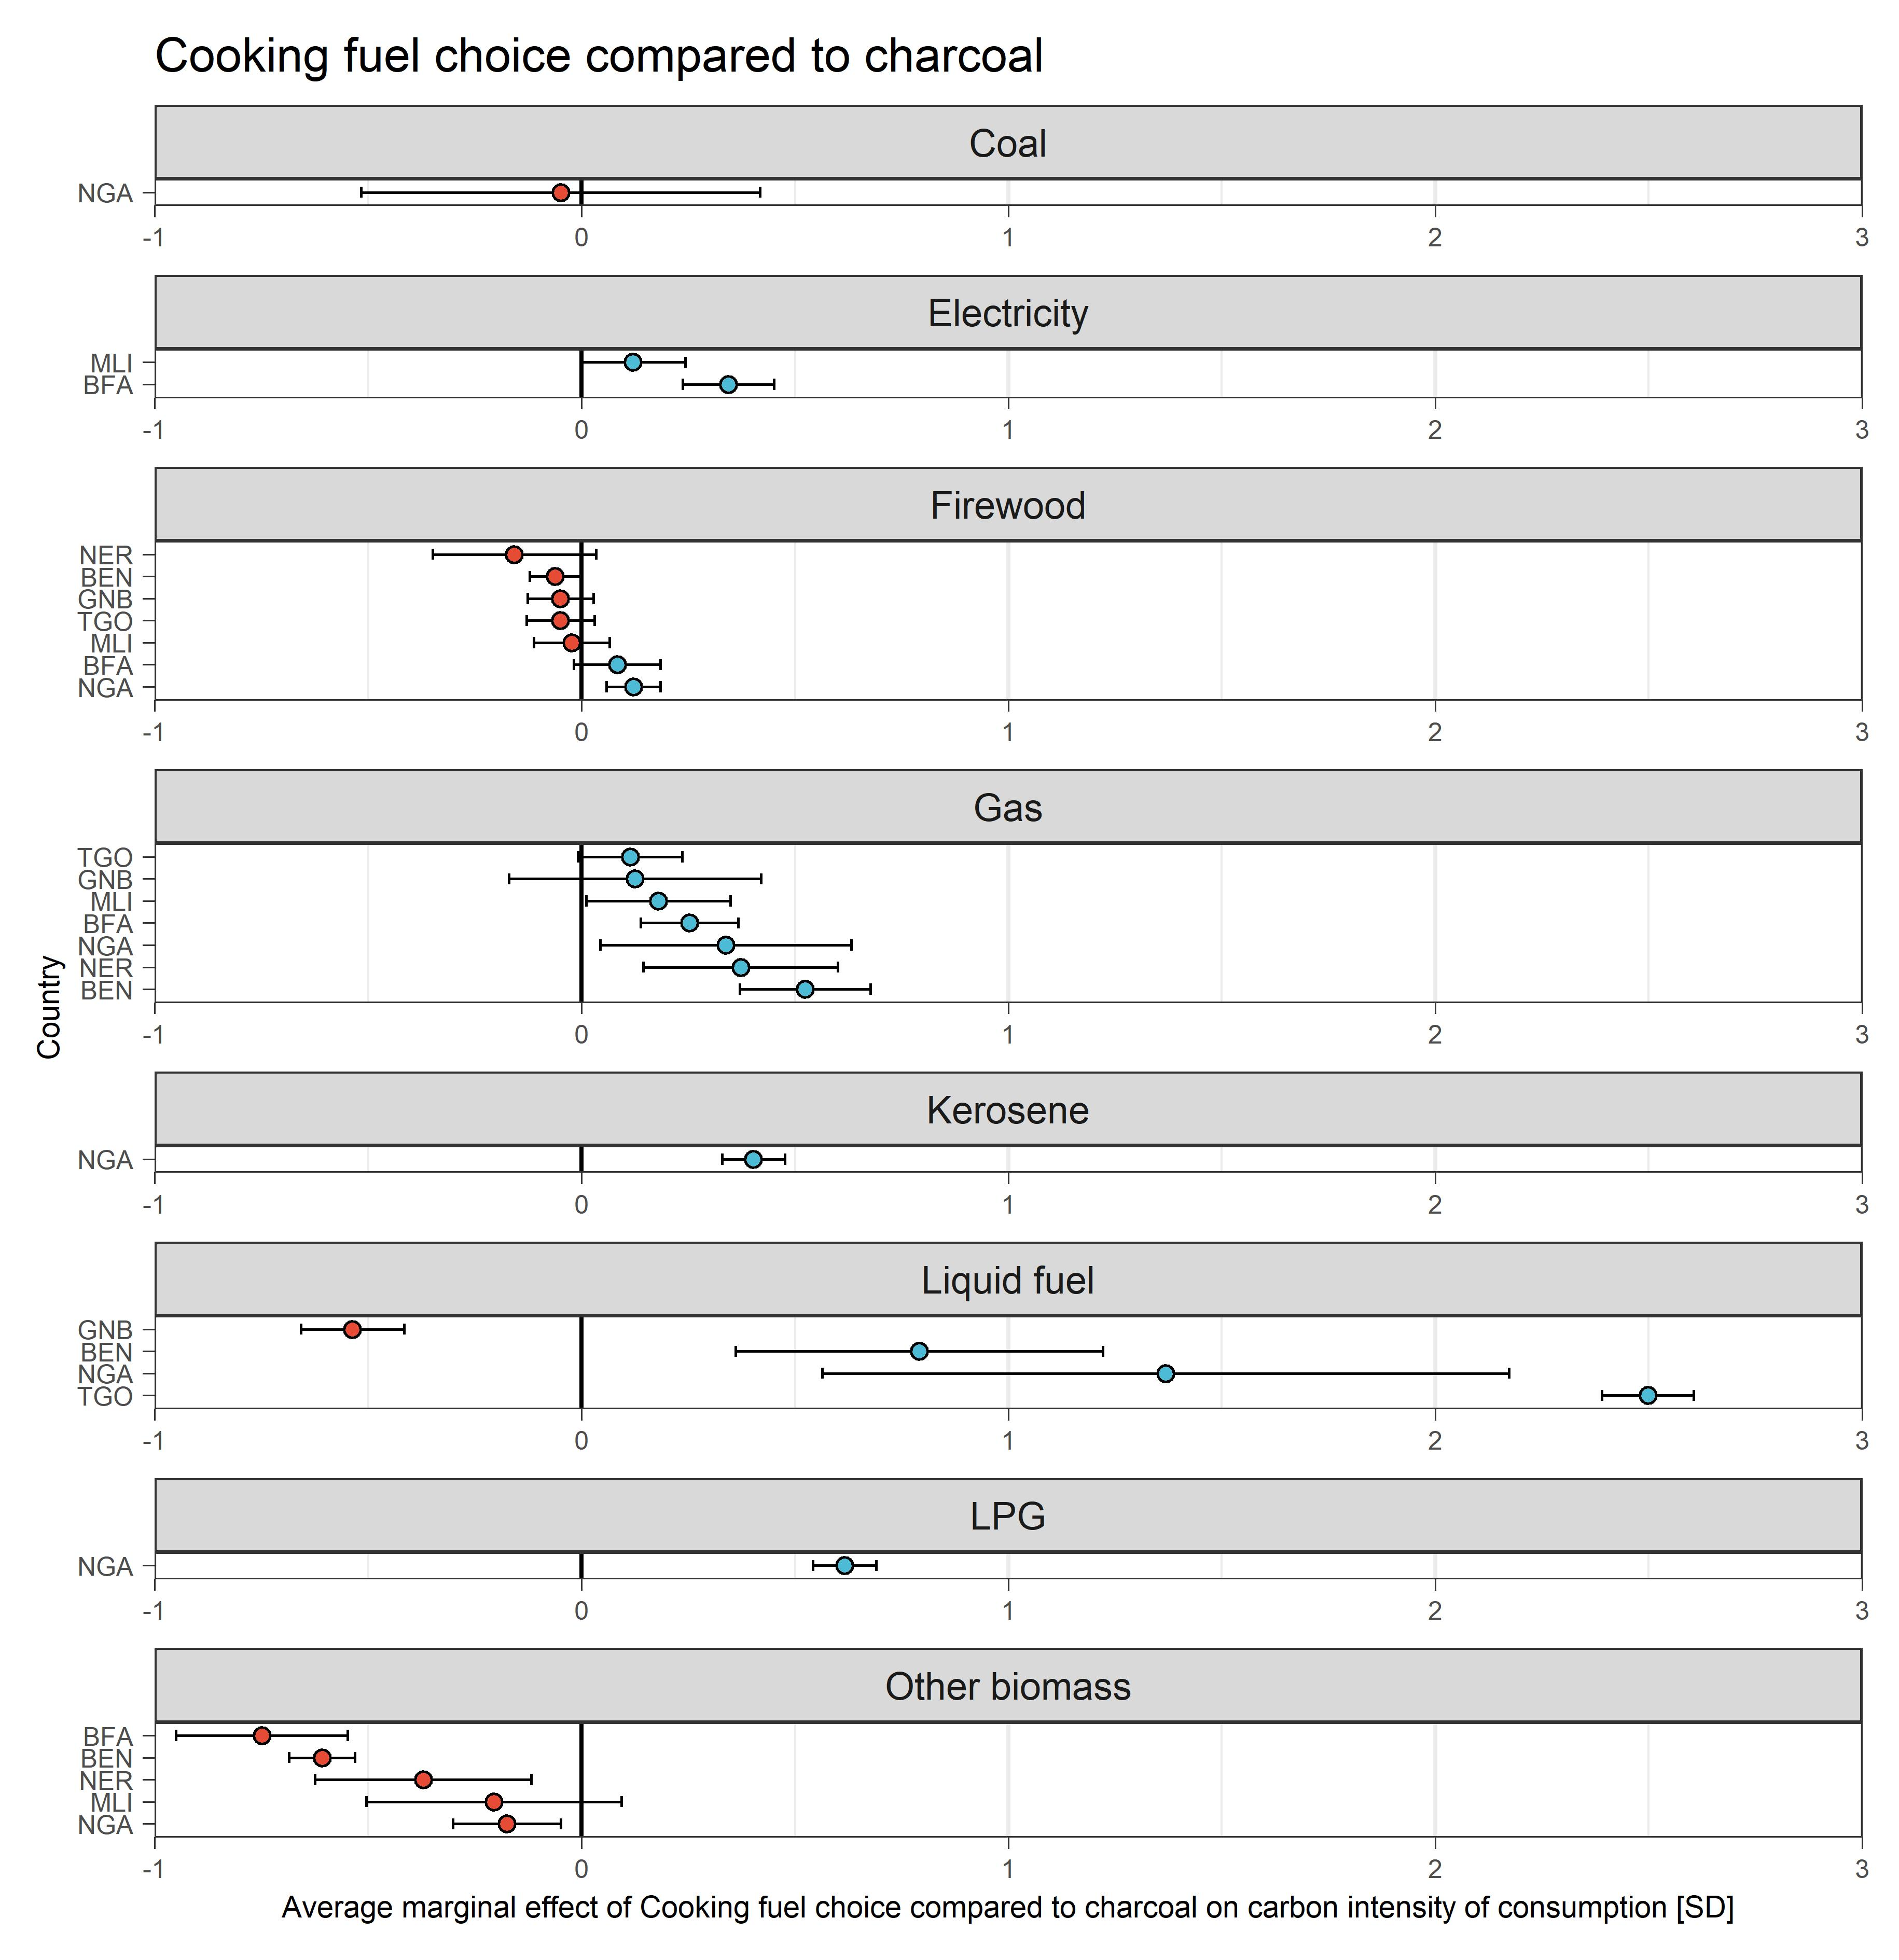
\includegraphics{Analysis_OLS_ME_Carbon_Intensity/AME_OLS_CI_CF_Charcoal}
%   \begin{subcaption}
%     This figure displays ...
%   \end{subcaption}

% \end{figure}

% \clearpage

% \begin{figure}[ht!]
%   \centering
%  \caption{Average marginal effects of secondary education} \label{fig:E10_sec_edu}
%   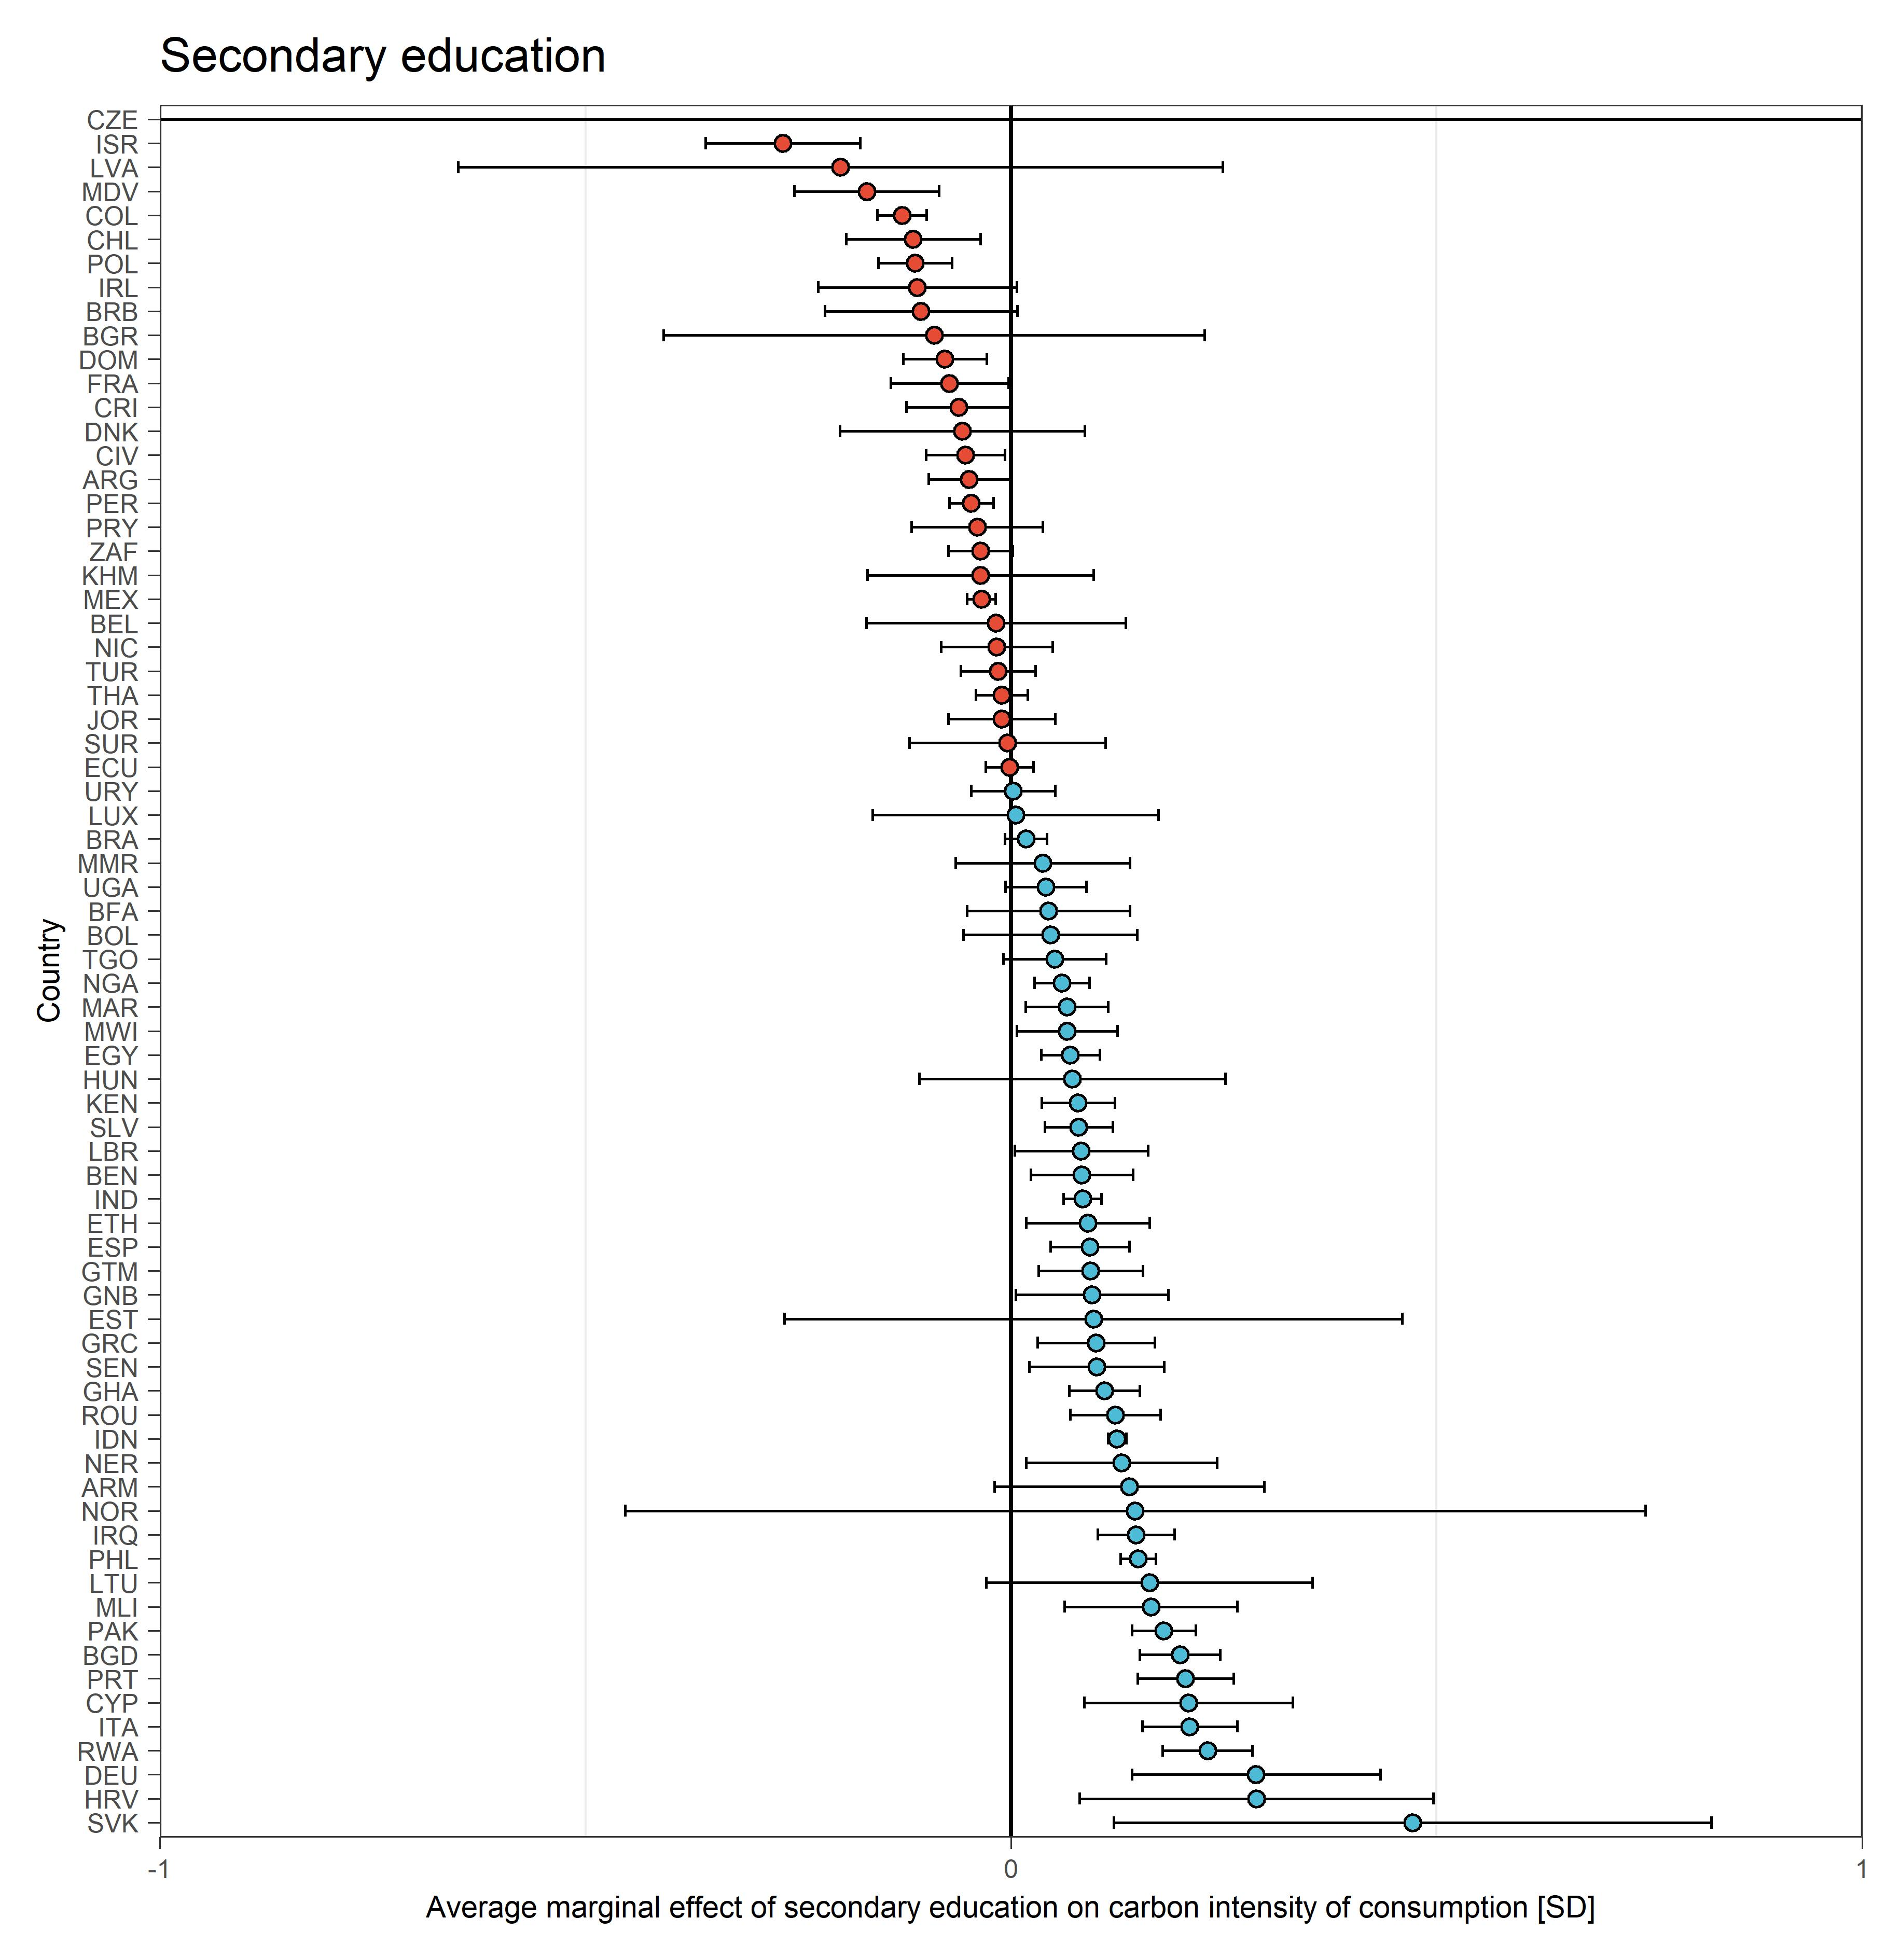
\includegraphics{Analysis_OLS_ME_Carbon_Intensity/AME_OLS_CI_secondary_education}
%   \begin{subcaption}
%     This figure displays ... Special case finland
%   \end{subcaption}

% \end{figure}

% \clearpage

% \begin{figure}[ht!]
%   \centering
%  \caption{Average marginal effects of higher education} \label{fig:E11_high_edu}
%   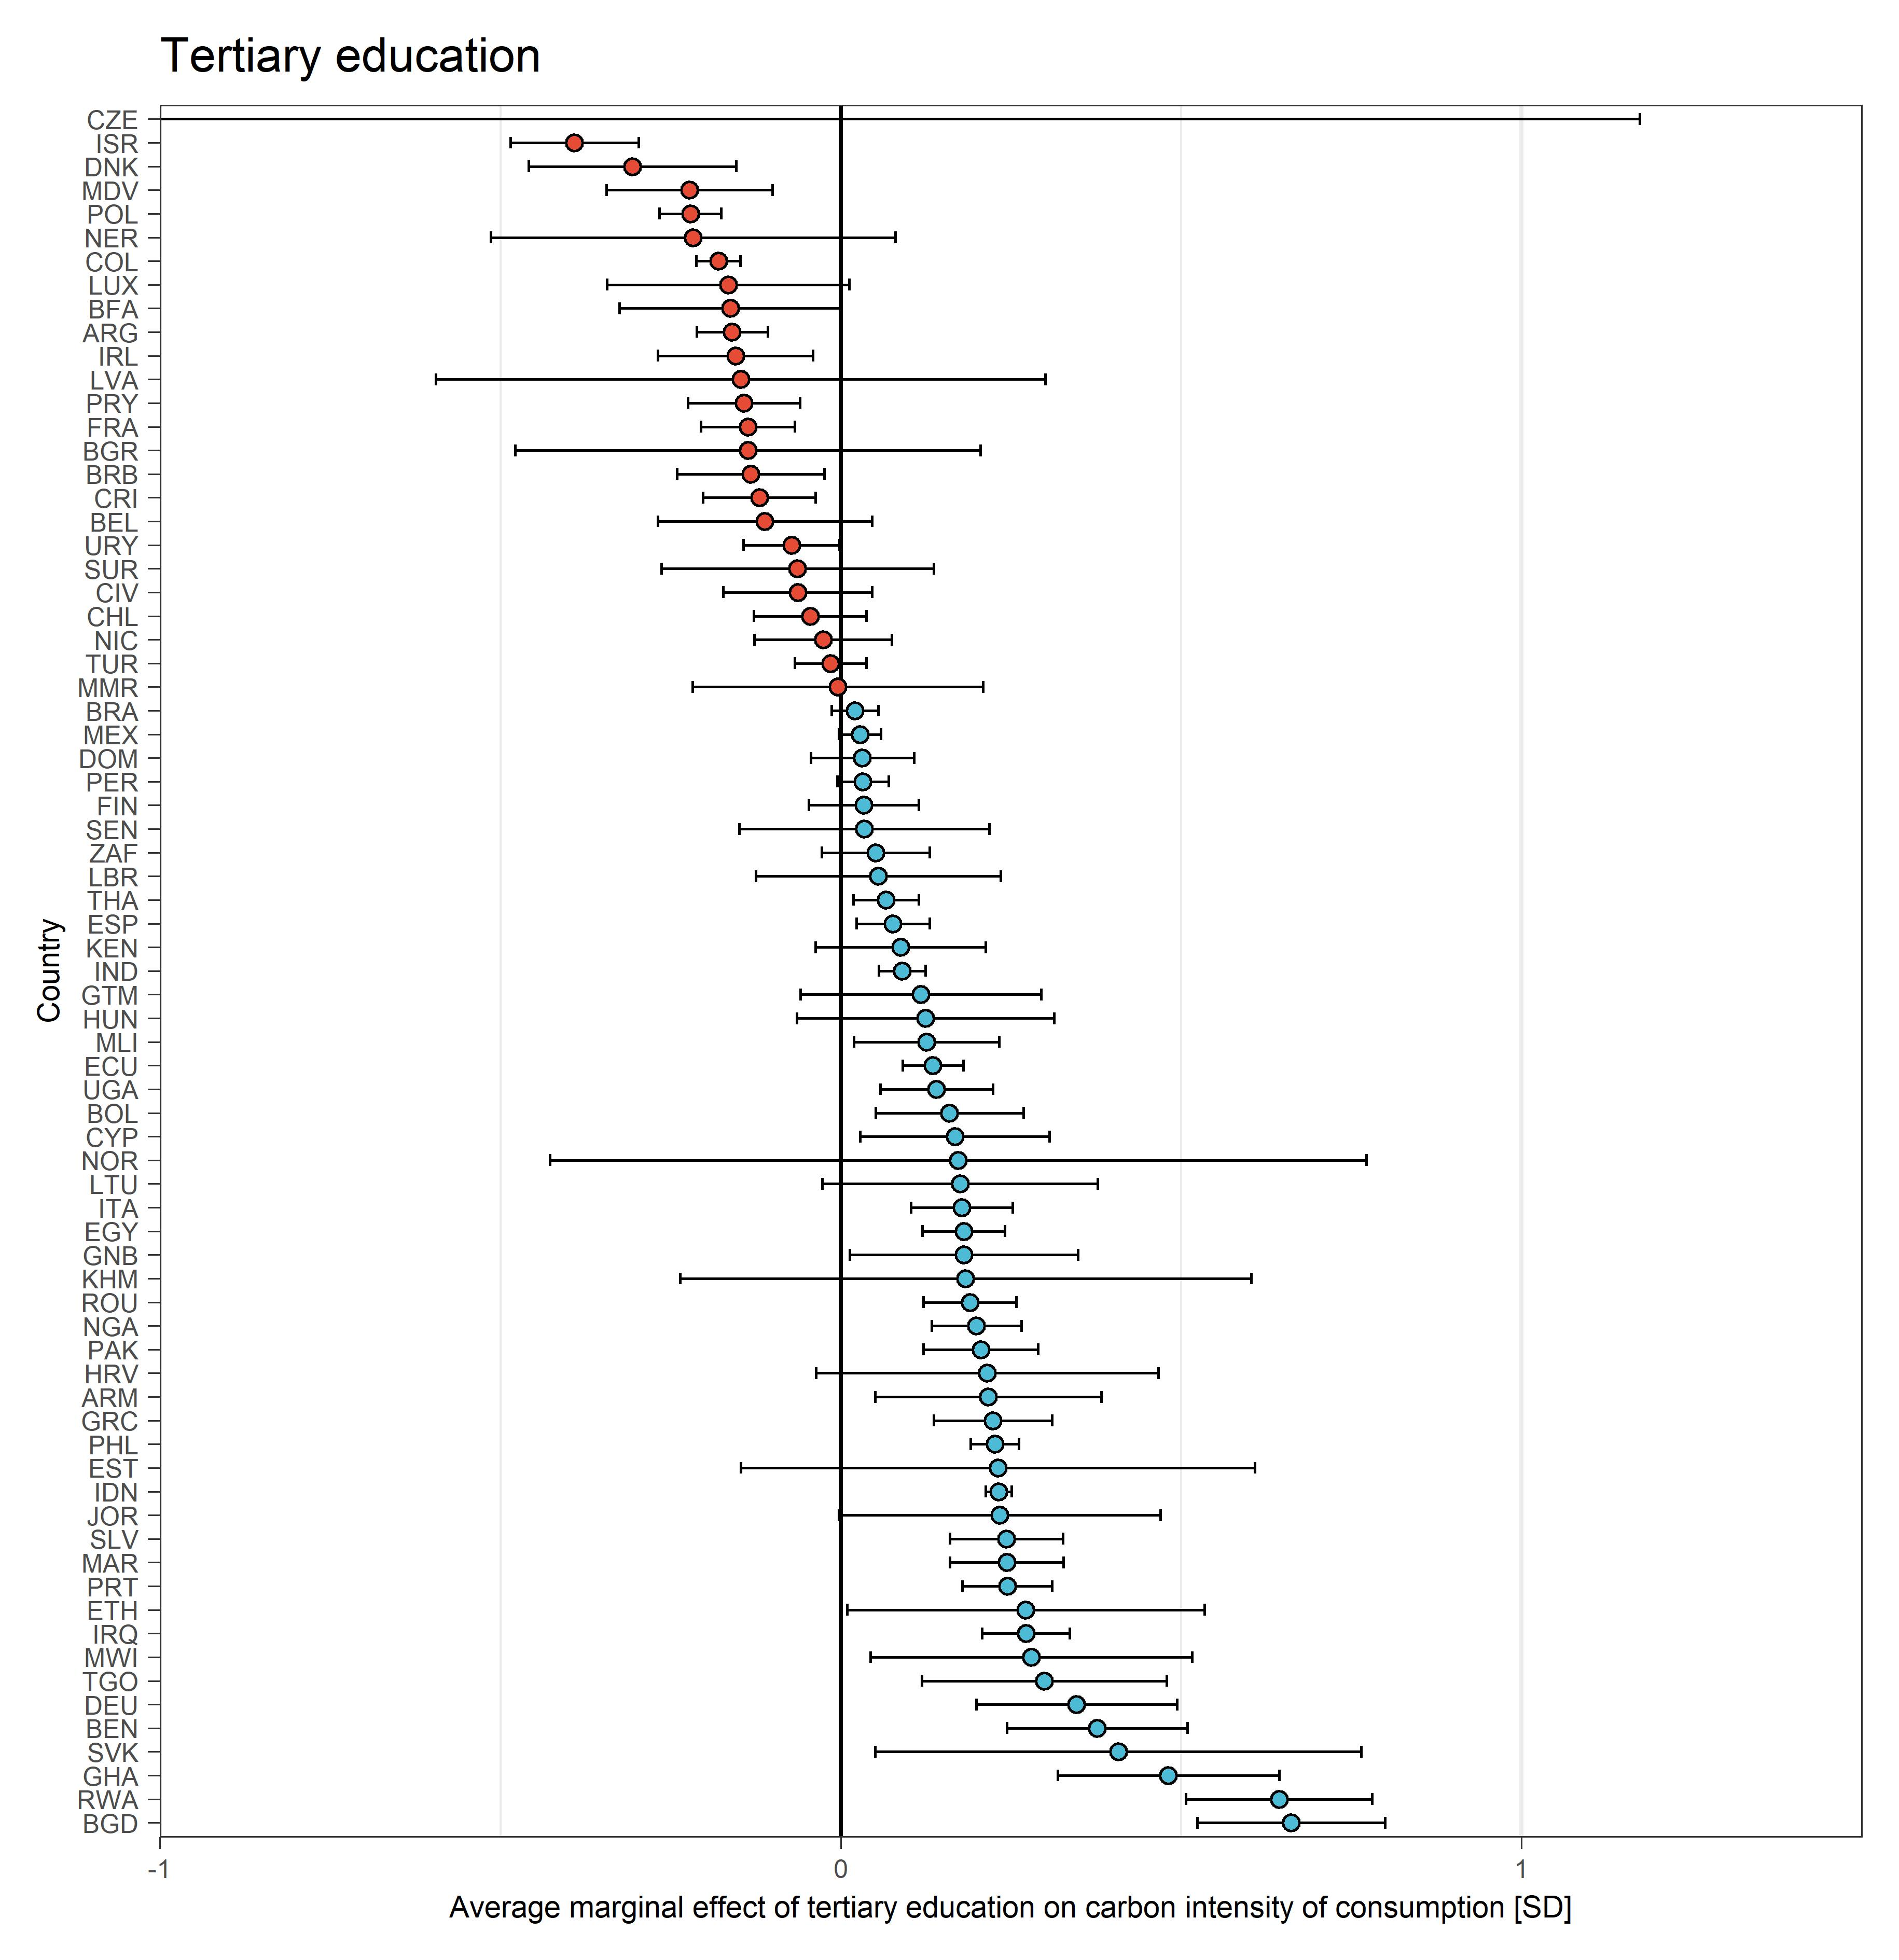
\includegraphics{Analysis_OLS_ME_Carbon_Intensity/AME_OLS_CI_higher_education}
%   \begin{subcaption}
%     This figure displays ... Special case finland
%   \end{subcaption}

% \end{figure}

% \clearpage

%  \begin{figure}[ht!]
%    \centering
%   \caption{Average marginal effects of car ownership} \label{fig:F1_Car}
%    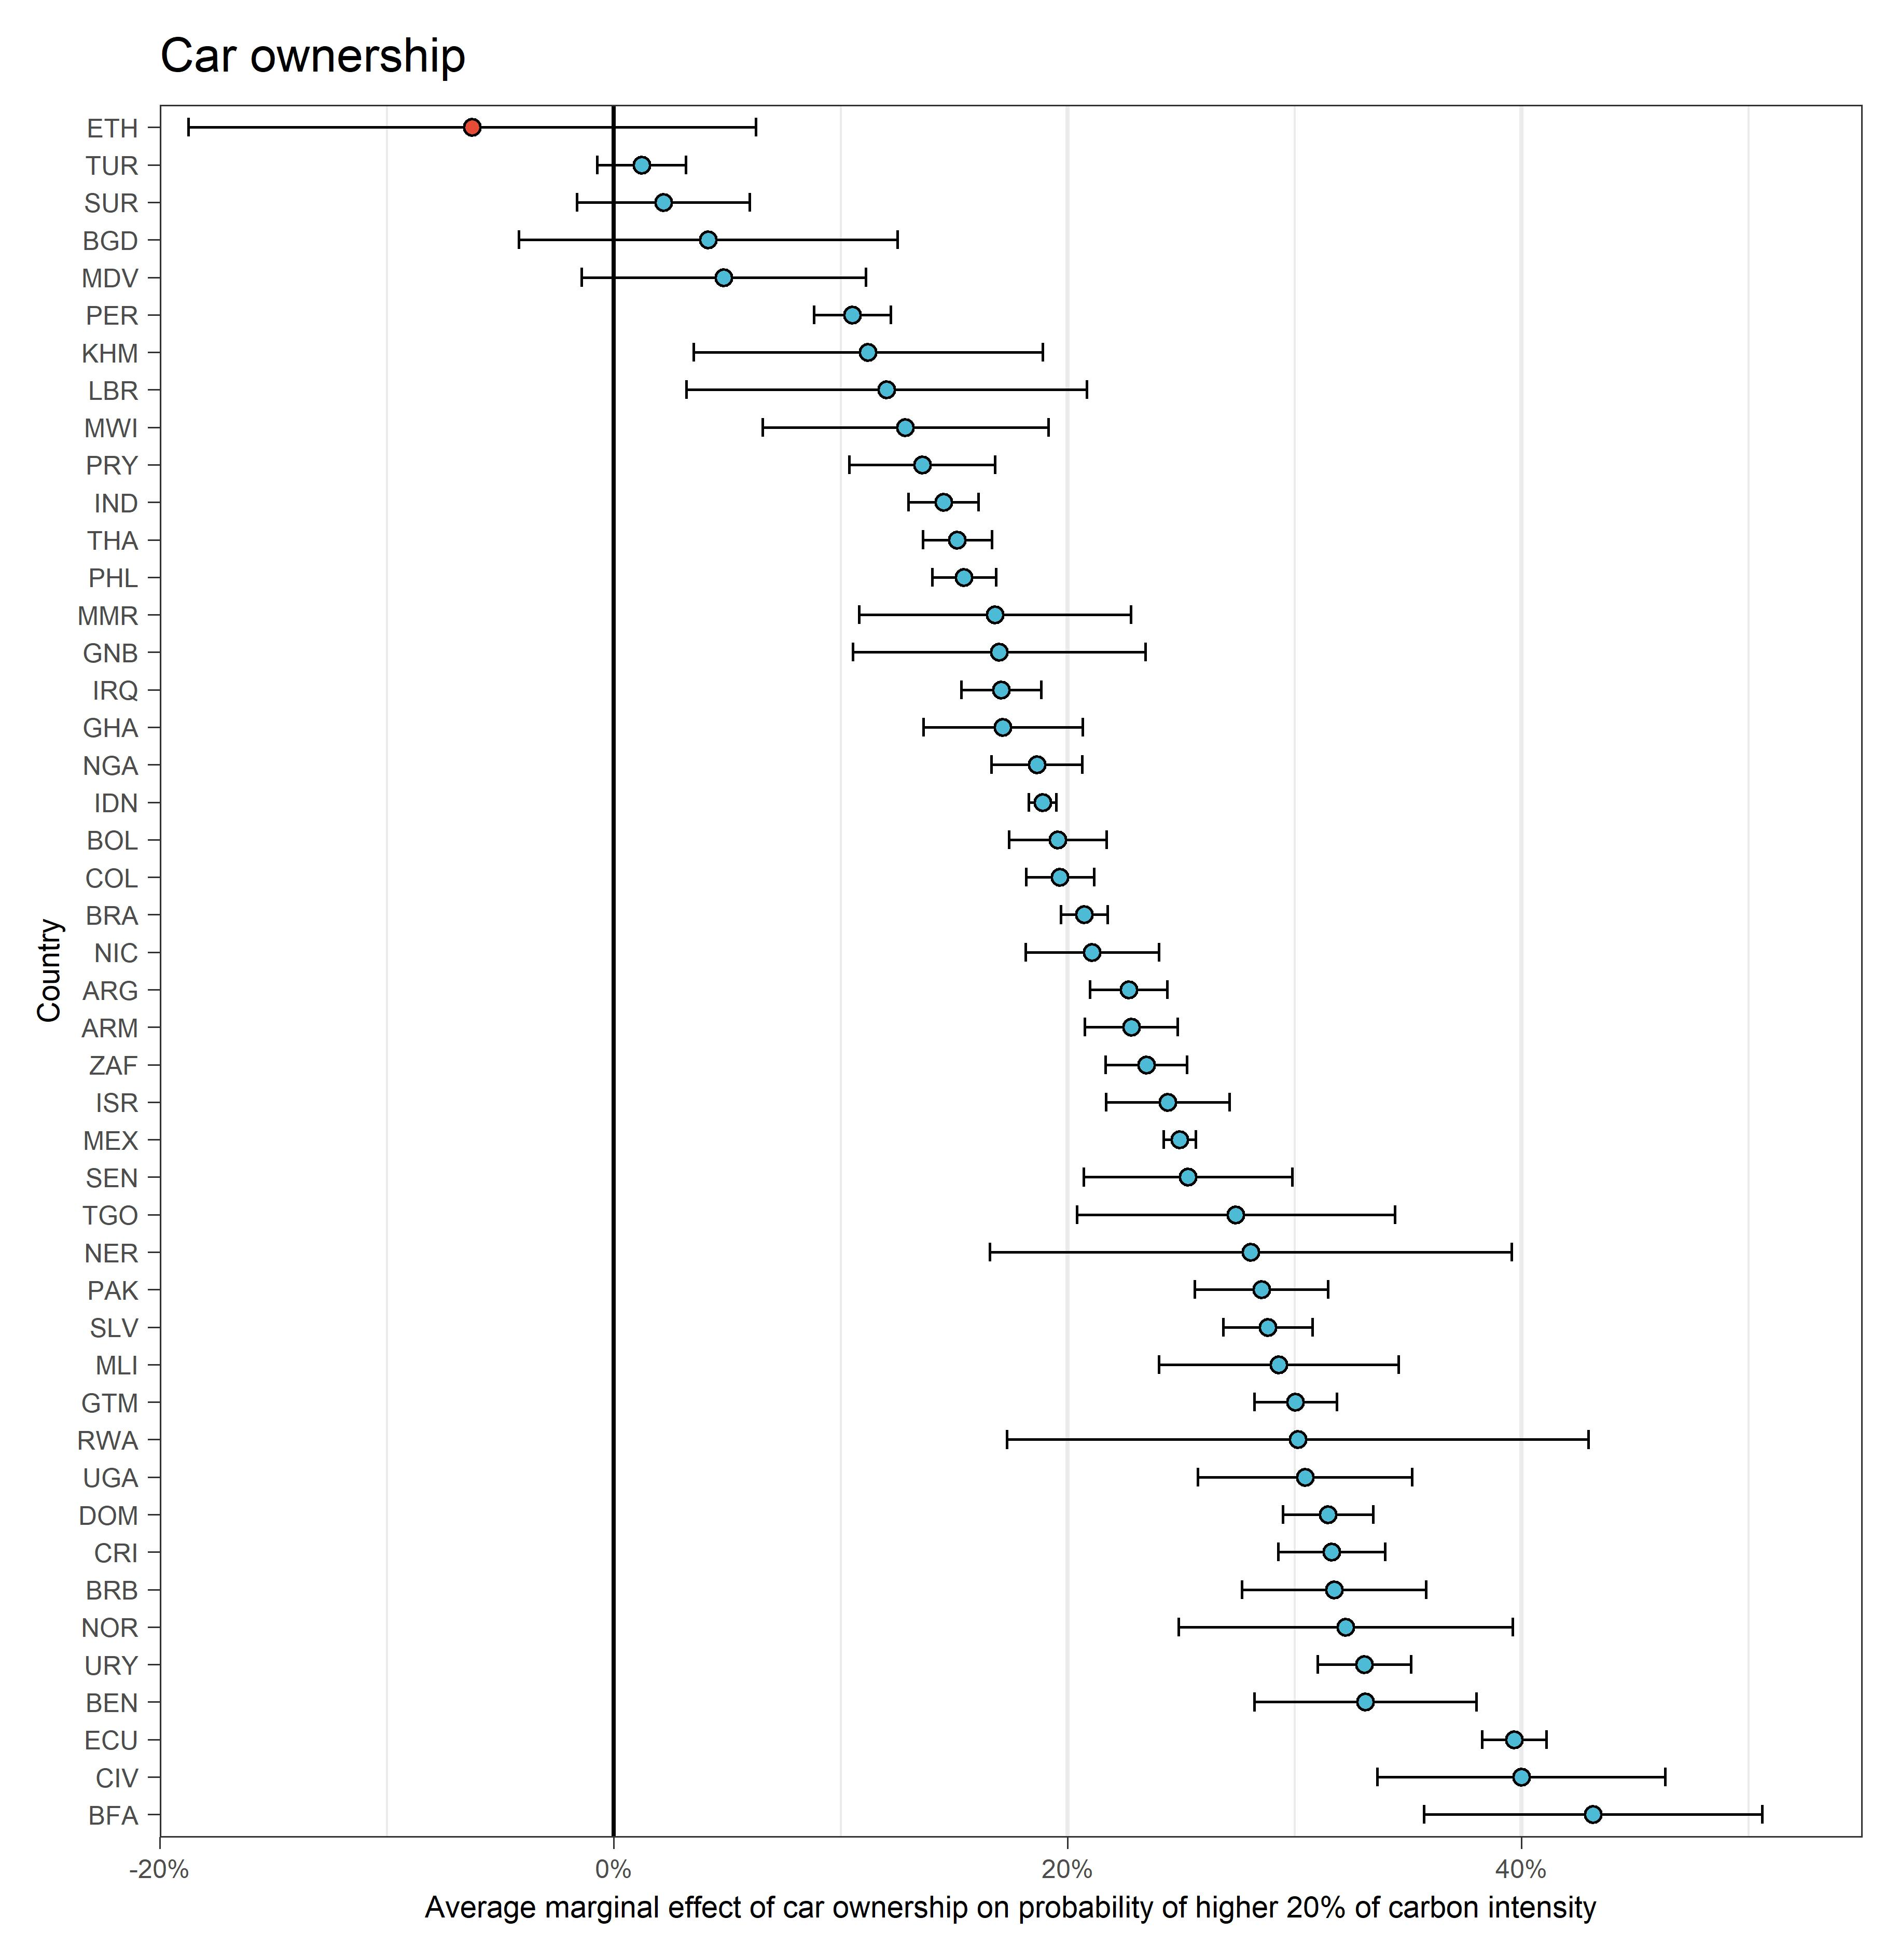
\includegraphics{Analysis_Logit_Models_Marginal_Effects/Average_Marginal_Effects_affected_upper_80_car.01}
%    \begin{subcaption}
%      This figure displays ...
%    \end{subcaption}

%  \end{figure}

%  \clearpage
% %
%  \begin{figure}[ht!]
%    \centering
%    \caption{Average marginal effects of electricity.access} \label{fig:F2_Electricity}
%    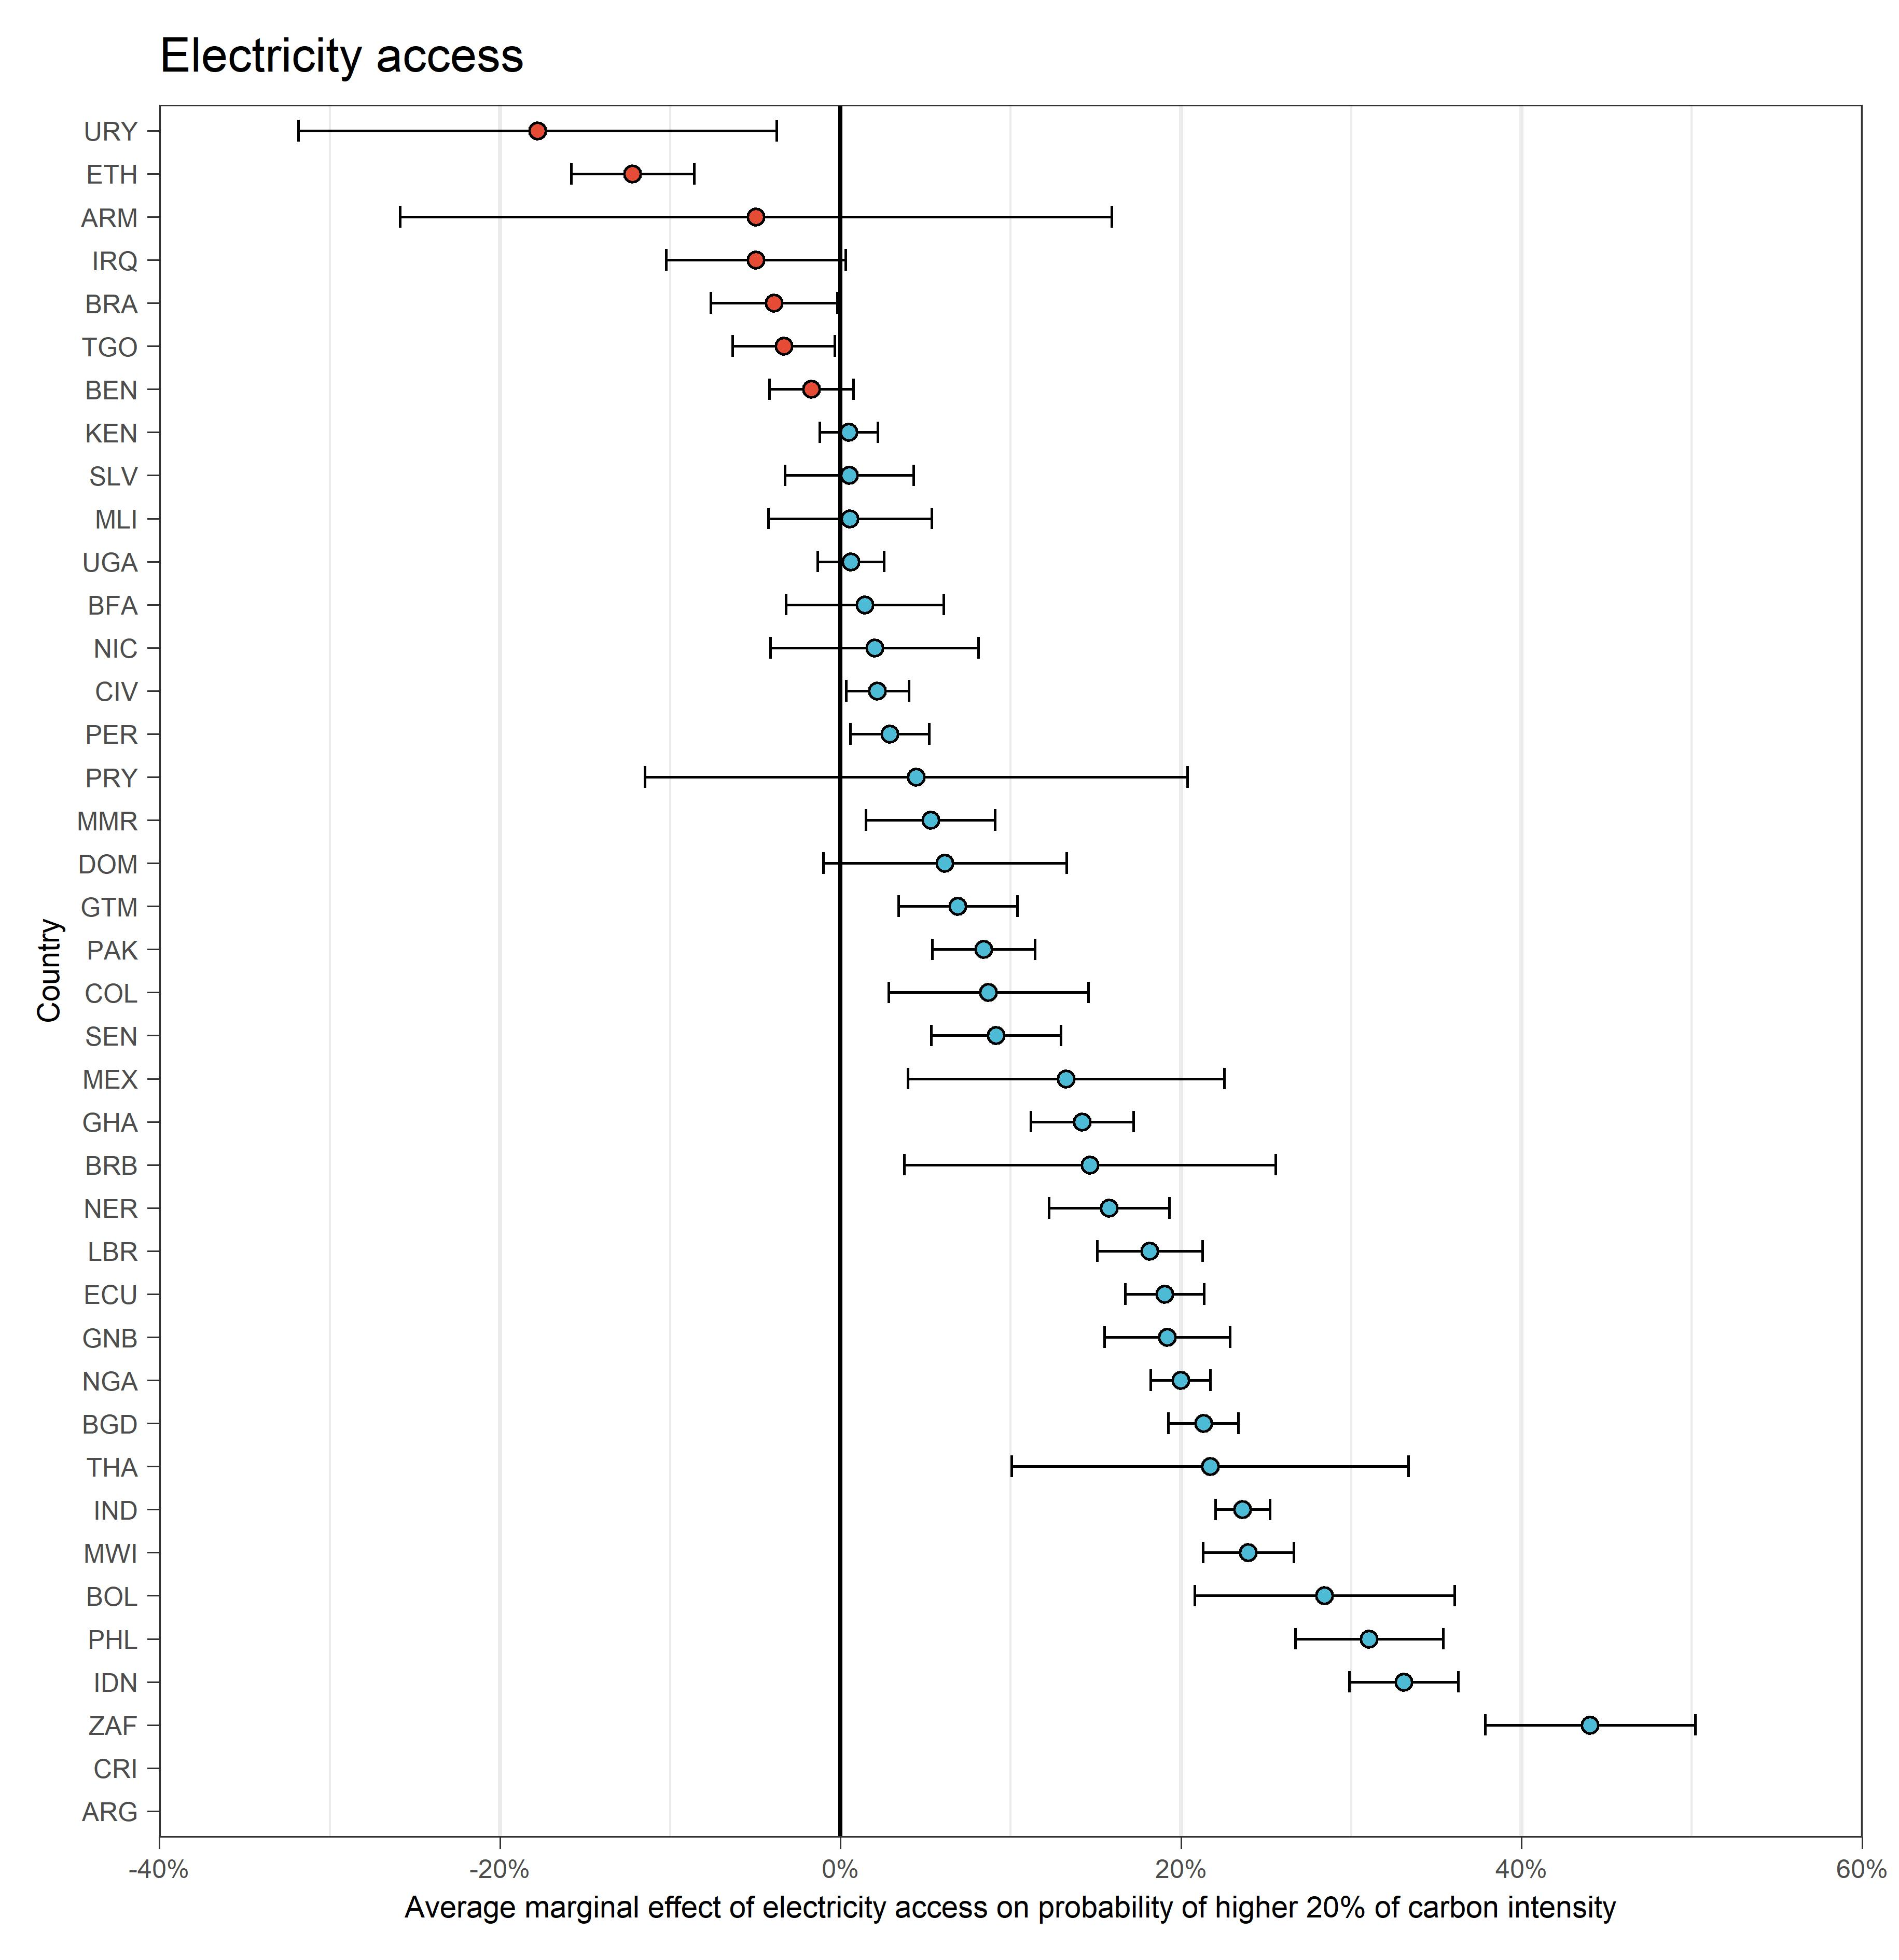
\includegraphics{Analysis_Logit_Models_Marginal_Effects/Average_Marginal_Effects_affected_upper_80_electricity.access}
%    \begin{subcaption}
%      This figure displays ...
%    \end{subcaption}
%  \end{figure}

%  \clearpage

%  \begin{figure}[ht!]
%    \centering
%    \caption{Average marginal effects of household size} \label{fig:F3_Size}
%    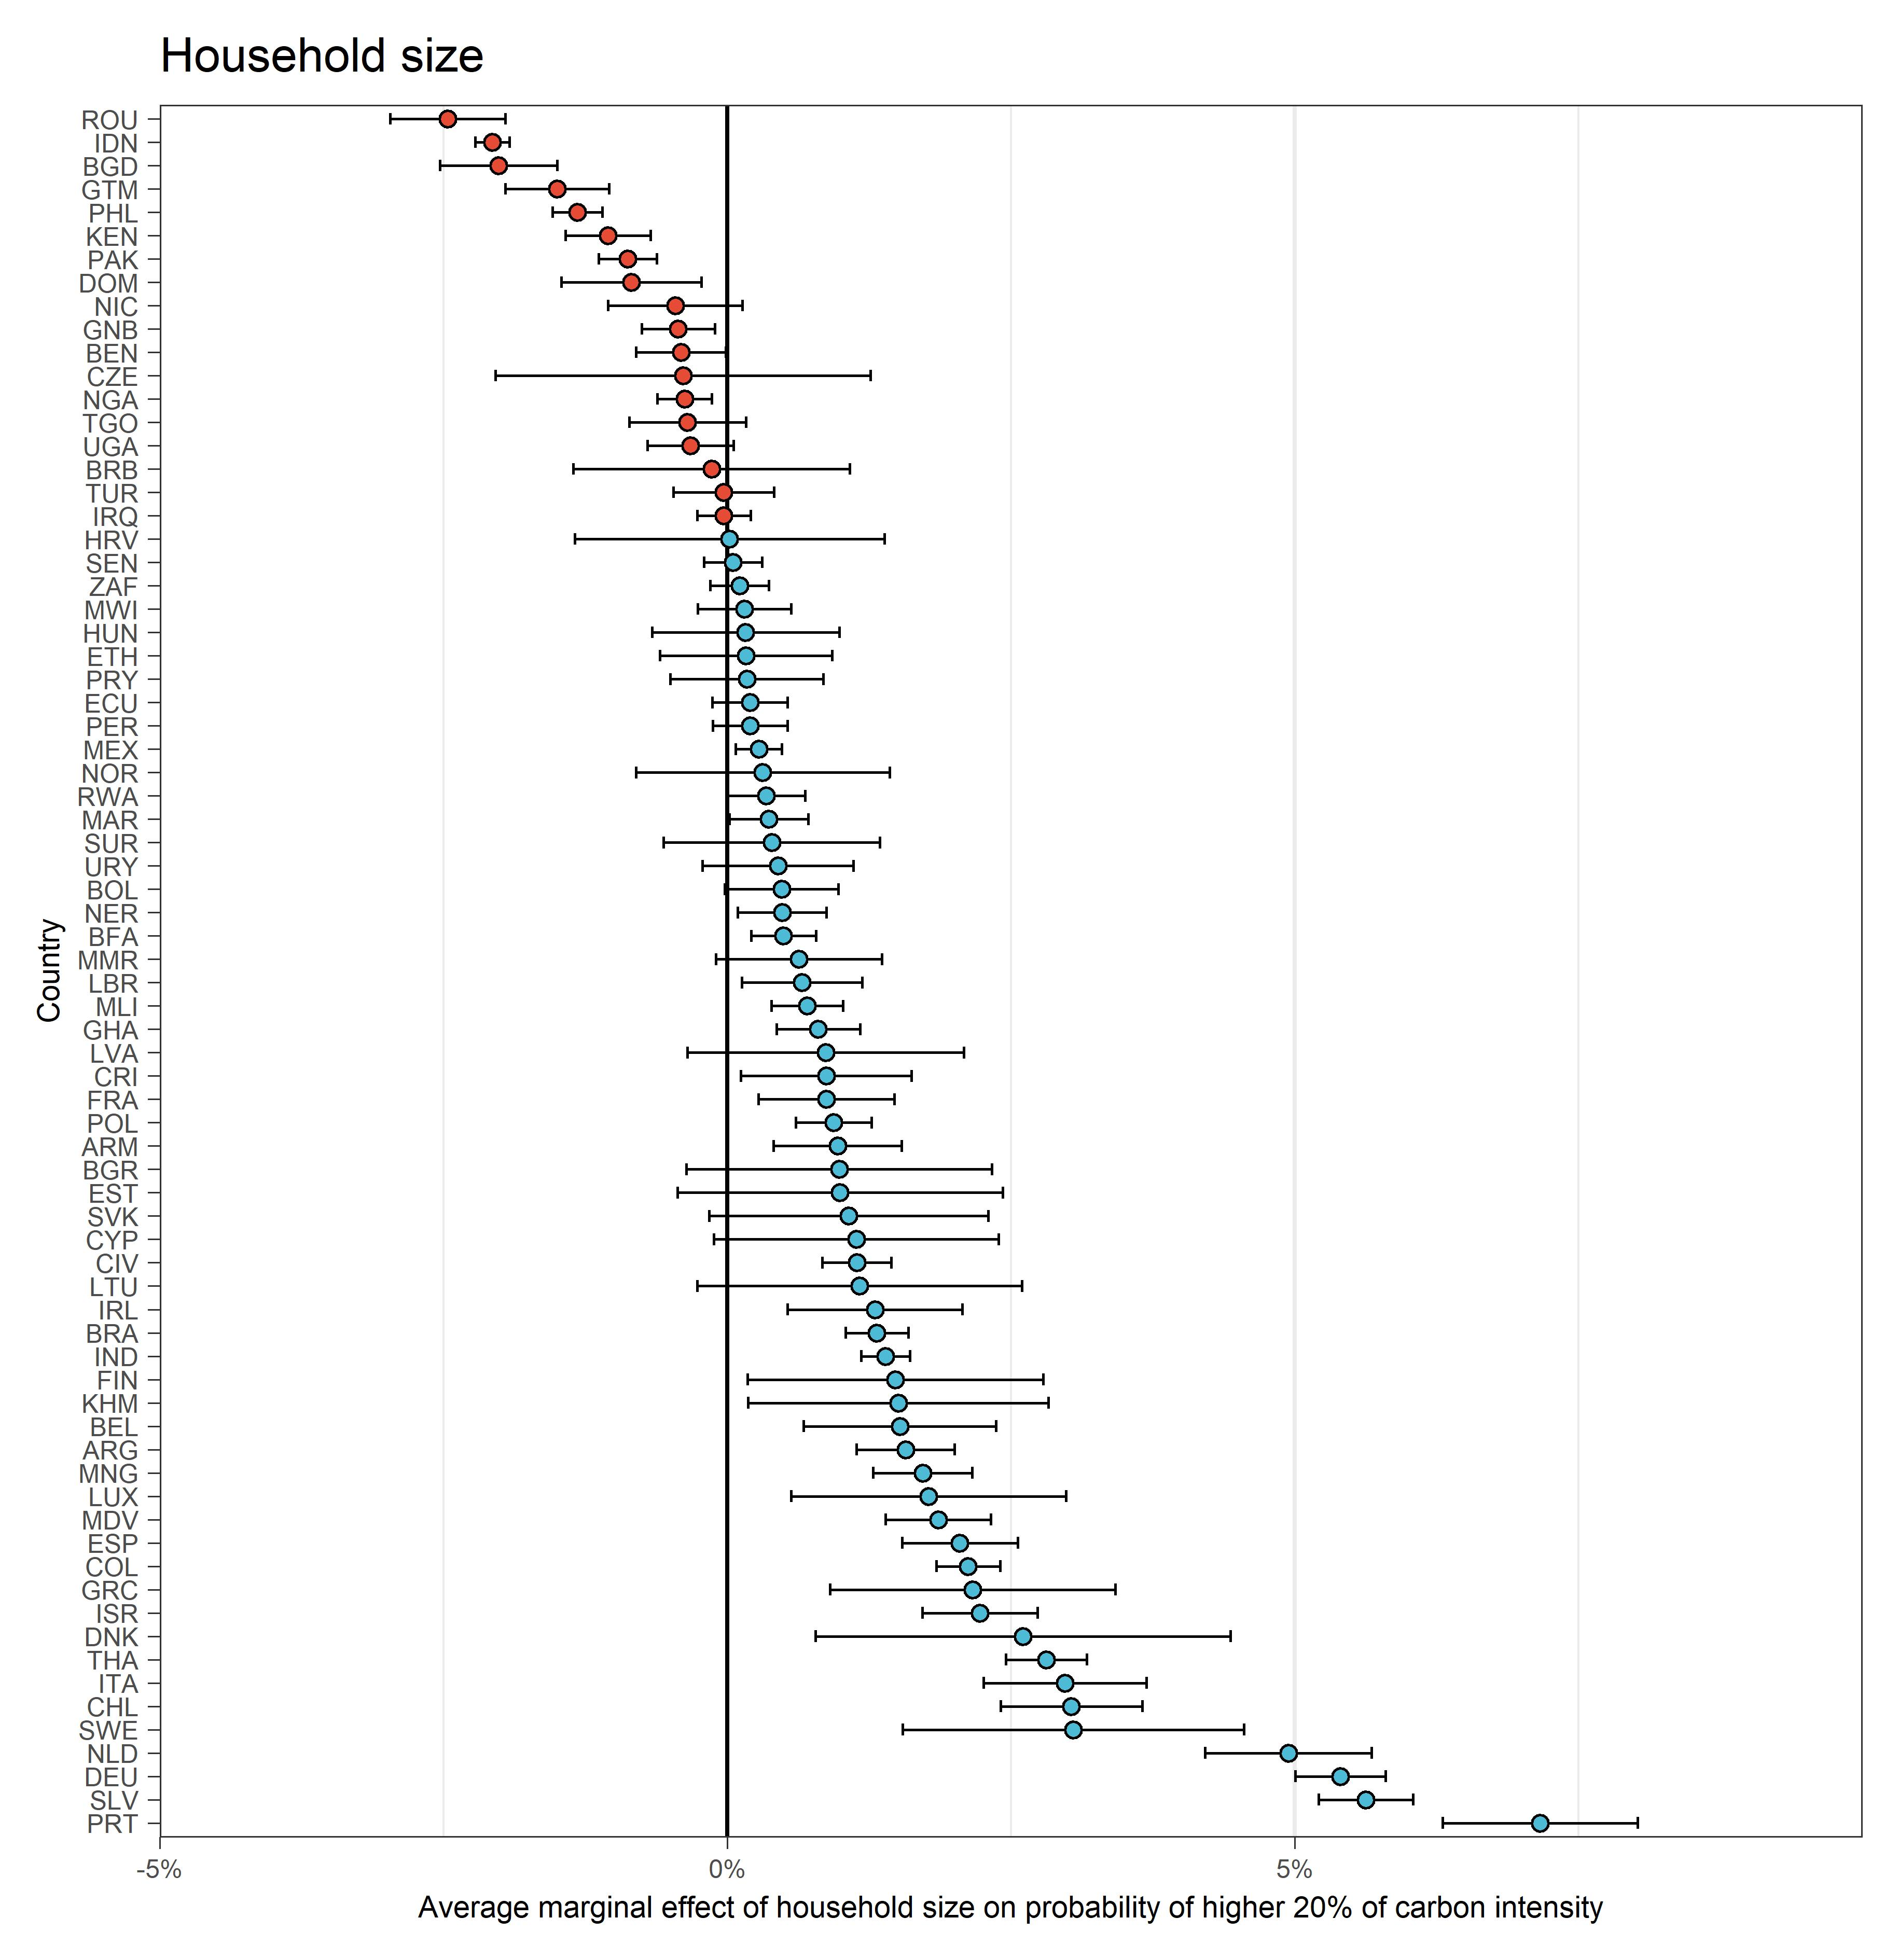
\includegraphics{Analysis_Logit_Models_Marginal_Effects/Average_Marginal_Effects_affected_upper_80_hh_size}
%    \begin{subcaption}
%      This figure displays ...
%    \end{subcaption}
%  \end{figure}

%  \clearpage

%  \begin{figure}[ht!]
%    \centering
%    \caption{Average marginal effects of household expenditures } \label{fig:F4_Expenditures}
%    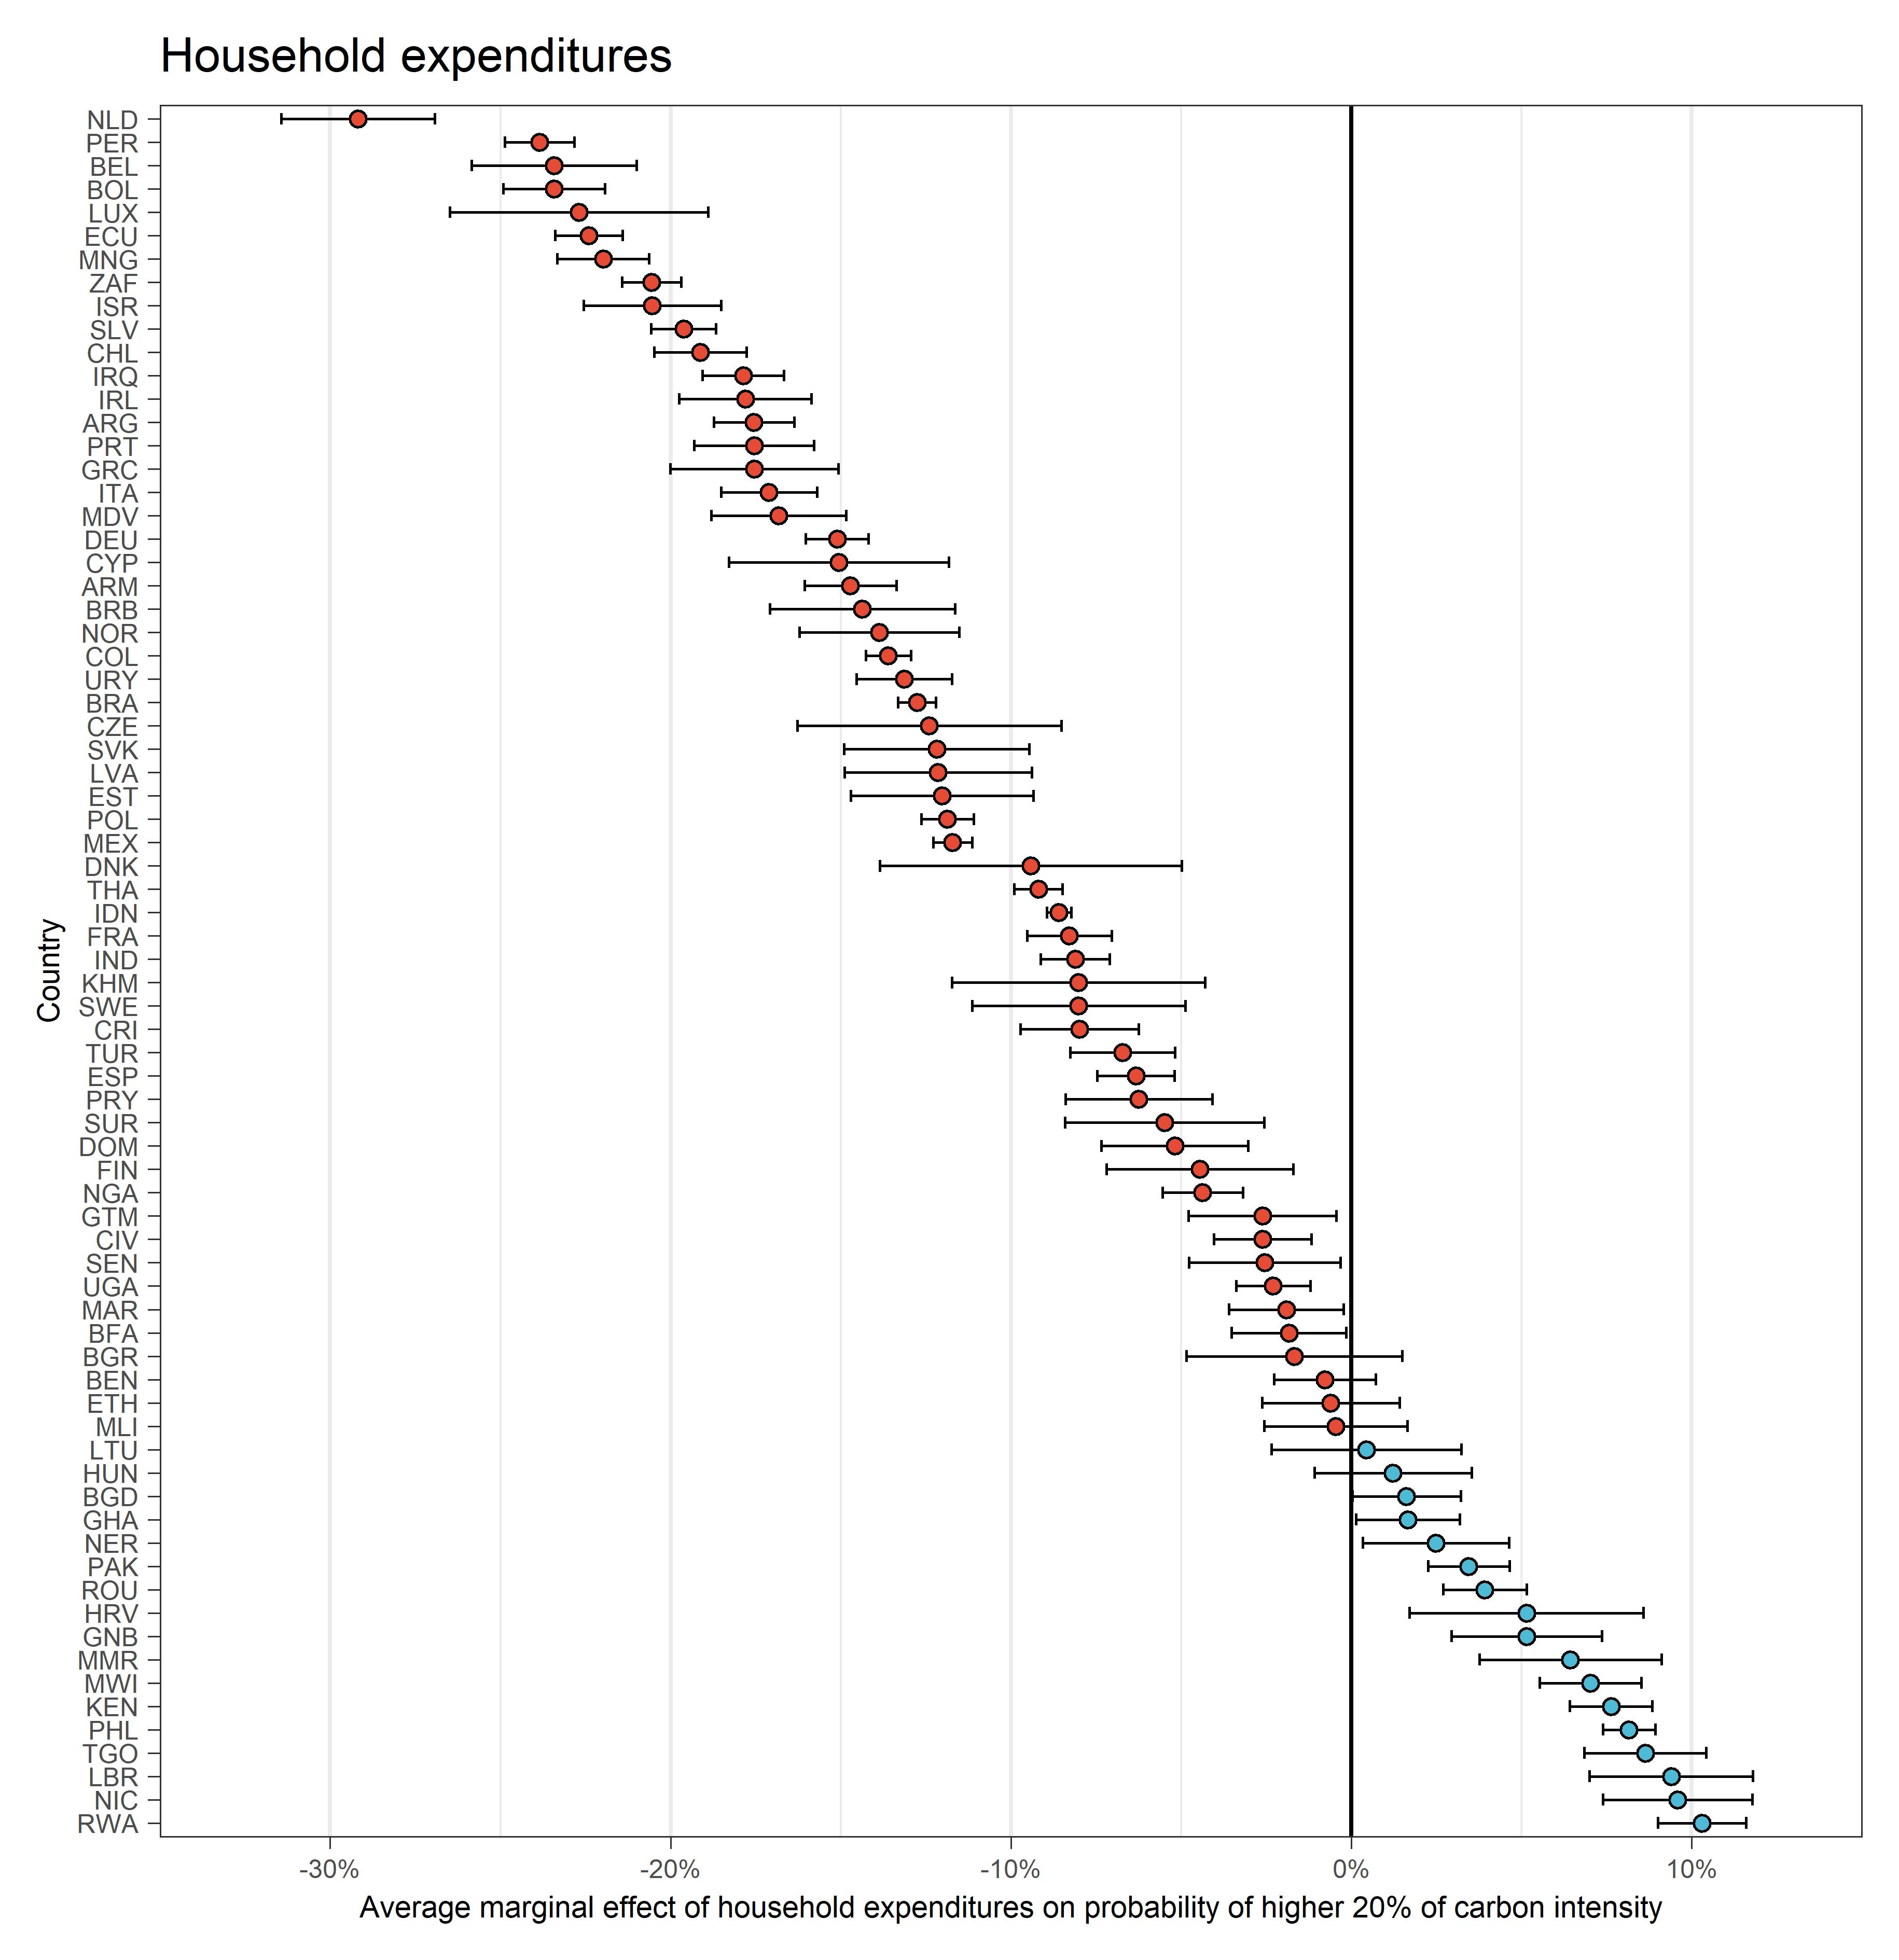
\includegraphics{Analysis_Logit_Models_Marginal_Effects/Average_Marginal_Effects_affected_upper_80_log_hh_expenditures_USD_2014}
%    \begin{subcaption}
%      This figure displays ...
%    \end{subcaption}
%  \end{figure}

%  \clearpage

%  \begin{figure}[ht!]
%    \centering
%    \caption{Average marginal effects of urban citizenship} \label{fig:F5_Urban}
%    \includegraphics{Analysis_Logit_Models_Marginal_Effects/Average_Marginal_Effects_affected_upper_80_urban_01}
%    \begin{subcaption}
%      This figure displays ...
%    \end{subcaption}
%  \end{figure}

%  \clearpage

%  \begin{figure}[ht!]
%    \centering
%    \caption{Average marginal effects of cooking fuel choice - Part A} \label{fig:F6_Electricity_A}
%    \includegraphics{Analysis_Logit_Models_Marginal_Effects/Average_Marginal_Effects_affected_upper_80_CF_Electricity A}
%    \begin{subcaption}
%      This figure displays ...
%    \end{subcaption}
%  \end{figure}

%  \clearpage

%  \begin{figure}[ht!]
%    \centering
%    \caption{Average marginal effects of cooking fuel choice - Part B} \label{fig:F7_Electricity_B}
%    \includegraphics{Analysis_Logit_Models_Marginal_Effects/Average_Marginal_Effects_affected_upper_80_CF_Electricity B}
%    \begin{subcaption}
%      This figure displays ...
%    \end{subcaption}
%  \end{figure}

%  \clearpage

%  \begin{figure}[ht!]
%    \centering
%    \caption{Average marginal effects of cooking fuel choice - Part C} \label{fig:F8_LPG}
%    \includegraphics{Analysis_Logit_Models_Marginal_Effects/Average_Marginal_Effects_affected_upper_80_CF_LPG}
%    \begin{subcaption}
%      This figure displays ...
%    \end{subcaption}
%  \end{figure}

%  \clearpage

%  \begin{figure}[ht!]
%    \centering
%    \caption{Average marginal effects of cooking fuel choice - Part D} \label{fig:F9_Charcoal}
%    \includegraphics{Analysis_Logit_Models_Marginal_Effects/Average_Marginal_Effects_affected_upper_80_CF_Charcoal}
%    \begin{subcaption}
%      This figure displays ...
%    \end{subcaption}
%  \end{figure}

%  \clearpage

%  \begin{figure}[ht!]
%    \centering
%    \caption{Average marginal effects of secondary education} \label{fig:F10_sec_edu}
%    \includegraphics{Analysis_Logit_Models_Marginal_Effects/Average_Marginal_Effects_affected_upper_80_secondary_education}
%    \begin{subcaption}
%      This figure displays ...
%    \end{subcaption}
%  \end{figure}

%  \clearpage

%  \begin{figure}[ht!]
%    \centering
%    \caption{Average marginal effects of higher education} \label{fig:F11_high_edu}
%    \includegraphics{Analysis_Logit_Models_Marginal_Effects/Average_Marginal_Effects_affected_upper_80_higher_education}
%    \begin{subcaption}
%      This figure displays ...
%    \end{subcaption}
%  \end{figure}

%  \clearpage

 \begin{figure}[ht!]
   \centering
   \caption{Average silhouette width for different number of clusters \textit{k}} \label{fig:G1_silhouette}
   \includegraphics{Figures_Appendix/Figure_Silhouette}
   \begin{subcaption}
     This figure displays ...
   \end{subcaption}
 \end{figure}

 \clearpage

 \begin{figure}[ht!]
   \centering
   \caption{Average silhouette width for each country per cluster \textit{k}} \label{fig:G2_silhouette}
   \includegraphics{Figures_Appendix/Figure_Silhouette_Clusters}
   \begin{subcaption}
     This figure displays ...
   \end{subcaption}
 \end{figure}

 \clearpage

\subsection{Supplementary tables} \label{sec:tables}

\begin{table}[H]

\caption{Summary statistics}
\centering
\resizebox{\linewidth}{!}{
\begin{threeparttable}
\begin{tabular}[t]{>{\raggedright\arraybackslash}p{3.5 cm}|>{\raggedleft\arraybackslash}p{2.3 cm}>{\centering\arraybackslash}p{2.3 cm}>{\centering\arraybackslash}p{2.3 cm}>{\centering\arraybackslash}p{2.3 cm}>{\raggedleft\arraybackslash}p{2.3 cm}>{\centering\arraybackslash}p{2.3 cm}>{\centering\arraybackslash}p{2.3 cm}}
\toprule
Country & Observations & Average 
Household Size & Urban 
Population & Electricity 
Access & Average 
Household 
Expenditures [USD] & Car 
Ownership & Share of 
Firewood or 
 Charcoal Cons.\\
\midrule
ARG & 21,539 & 3.19 &  & 99.9\% & 14,437 & 49\% & 5\%\\
ARM & 7,776 & 3.63 & 66\% & 99.8\% & 5,371 & 32\% & 1\%\\
BEL & 6,135 & 2.31 & 96\% & NaN\% & 36,297 &  & 9\%\\
BEN & 8,012 & 5.21 & 47\% & 33.1\% & 3,127 & 3\% & 97\%\\
BFA & 7,010 & 6.51 & 31\% & 24.4\% & 3,095 & 4\% & 92\%\\
BGD & 12,240 & 4.50 & 27\% & 55.2\% & 2,125 & 1\% & 39\%\\
BGR & 2,966 & 2.37 & 71\% & NaN\% & 6,376 &  & 37\%\\
BOL & 11,859 & 3.34 & 69\% & 94.7\% & 3,688 & 17\% & 12\%\\
BRA & 57,889 & 3.01 & 86\% & 99.5\% & 12,247 & 46\% & 3\%\\
BRB & 2,434 & 2.62 &  & 94.7\% & 16,842 & 52\% & 0\%\\
CHL & 15,237 & 3.29 &  & NaN\% & 19,547 &  & 11\%\\
CIV & 12,992 & 4.48 & 52\% & 64.1\% & 3,718 & 3\% & 77\%\\
COL & 86,866 & 3.35 & 79\% & 98.3\% & 8,586 & 14\% & 9\%\\
CRI & 7,046 & 3.24 & 71\% & 99.7\% & 12,177 & 45\% & 5\%\\
CYP & 2,876 & 2.70 & 74\% & NaN\% & 31,922 &  & 21\%\\
CZE & 2,929 & 2.22 & 67\% & NaN\% & 12,615 &  & 22\%\\
DEU & 52,412 & 2.00 & 90\% & NaN\% & 32,812 &  & 0\%\\
DNK & 2,205 & 2.12 & 67\% & NaN\% & 43,812 &  & 21\%\\
DOM & 8,884 & 3.21 & 81\% & 97.5\% & 7,786 & 21\% & 7\%\\
ECU & 28,263 & 3.68 & 69\% & 90.5\% & 6,432 & 19\% & 5\%\\
ESP & 22,127 & 2.50 & 75\% & NaN\% & 26,216 &  & 0\%\\
EST & 3,395 & 2.24 & 51\% & NaN\% & 13,491 &  & 33\%\\
ETH & 6,767 & 4.48 & 32\% & 55.9\% & 1,100 & 1\% & 96\%\\
FIN & 3,673 & 2.02 & 71\% & NaN\% & 36,791 &  & 43\%\\
FRA & 16,978 & 2.23 & 69\% & NaN\% & 31,107 &  & 0\%\\
GHA & 13,521 & 3.91 & 56\% & 83.1\% & 2,312 & 4\% & 83\%\\
GNB & 5,351 & 8.18 & 47\% & 21.7\% & 4,172 & 3\% & 99\%\\
GRC & 6,150 & 2.58 & 72\% & NaN\% & 22,585 &  & 28\%\\
GTM & 11,534 & 4.77 & 54\% & 81\% & 4,830 & 17\% & 70\%\\
HRV & 2,029 & 2.89 & 59\% & NaN\% & 14,048 &  & 51\%\\
HUN & 7,185 & 2.34 & 56\% & NaN\% & 9,596 &  & 42\%\\
IDN & 295,116 & 3.77 & 55\% & 98.5\% & 2,799 & 11\% & 29\%\\
IND & 101,581 & 4.43 & 31\% & 79.9\% & 1,514 & 4\% & 63\%\\
IRL & 6,839 & 2.73 & 65\% & NaN\% & 39,751 &  & 31\%\\
IRQ & 24,994 & 6.73 & 72\% & 99.3\% & 13,940 & 35\% & 3\%\\
ISR & 8,786 & 3.28 & 90\% & NaN\% & 39,641 & 72\% & 0\%\\
ITA & 15,010 & 2.34 & 82\% & NaN\% & 27,521 &  & 15\%\\
KEN & 21,714 & 3.98 & 44\% & 56.4\% & 2,372 &  & 82\%\\
KHM & 1,206 & 4.34 & 27\% & NaN\% & 5,263 & 11\% & 73\%\\
LBR & 8,332 & 4.27 & 52\% & 16.7\% & 2,617 & 2\% & 99\%\\
LTU & 3,443 & 2.15 & 47\% & NaN\% & 10,068 &  & 33\%\\
LUX & 3,167 & 2.42 & 81\% & NaN\% & 57,666 &  & 0\%\\
LVA & 3,844 & 2.37 & 56\% & NaN\% & 11,616 &  & 0\%\\
MAR & 15,970 & 4.74 & 65\% & NaN\% & 8,194 &  & 21\%\\
MDV & 4,749 & 5.19 &  & NaN\% & 19,238 & 5\% & 0\%\\
MEX & 88,899 & 3.55 & 79\% & 99.7\% & 6,846 & 40\% & 15\%\\
MLI & 6,602 & 7.14 & 28\% & 27.5\% & 4,011 & 4\% & 99\%\\
MMR & 3,648 & 4.53 & 29\% & 63\% & 2,541 & 4\% & 88\%\\
MNG & 11,197 & 3.58 & 66\% & NaN\% & 7,174 &  & 44\%\\
MWI & 11,374 & 4.40 & 16\% & 10.7\% & 734 & 2\% & 99\%\\
NER & 6,024 & 5.96 & 17\% & 15.7\% & 2,206 & 2\% & 97\%\\
NGA & 22,110 & 5.08 & 40\% & 63.4\% & 3,955 & 8\% & 70\%\\
NIC & 6,850 & 4.38 & 60\% & 86.8\% & 4,985 & 8\% & 51\%\\
NLD & 14,408 & 2.19 & 90\% & NaN\% & 39,679 &  & 1\%\\
NOR & 3,363 & 2.77 & 82\% & NaN\% & 64,706 & 88\% & 0\%\\
PAK & 17,986 & 6.35 & 36\% & 91.5\% & 862 & 4\% & 20\%\\
PER & 34,542 & 3.56 & 77\% & 95.6\% & 4,866 & 12\% & 15\%\\
PHL & 41,540 & 4.60 & 44\% & 91.1\% & 4,838 & 7\% & 45\%\\
POL & 37,148 & 2.80 & 64\% & NaN\% & 14,962 &  & 6\%\\
PRT & 11,398 & 2.53 & 73\% & NaN\% & 20,295 &  & 9\%\\
PRY & 5,410 & 3.90 & 61\% & 97.8\% & 8,371 & 25\% & 29\%\\
ROU & 30,625 & 2.66 & 58\% & NaN\% & 6,039 &  & 9\%\\
RWA & 14,577 & 4.39 & 19\% & NaN\% & 1,353 & 1\% & 41\%\\
SEN & 7,156 & 8.91 & 53\% & 63.7\% & 7,639 & 5\% & 86\%\\
SLV & 23,622 & 3.67 & 64\% & 95.7\% & 5,707 & 15\% & 12\%\\
SUR & 2,025 & 3.39 & 72\% & NaN\% & 8,490 & 38\% & 0\%\\
SVK & 4,785 & 2.93 & 71\% & NaN\% & 15,012 &  & 19\%\\
SWE & 2,871 & 2.13 & 45\% & NaN\% & 33,704 &  & 0\%\\
TGO & 6,171 & 4.23 & 47\% & 51.8\% & 2,733 & 3\% & 92\%\\
THA & 42,711 & 3.04 & 36\% & 99.8\% & 3,917 & 14\% & 26\%\\
TUR & 10,060 & 3.64 & 70\% & NaN\% & 12,906 & 39\% & 4\%\\
UGA & 15,627 & 4.82 & 28\% & 39.2\% & 1,494 & 3\% & 95\%\\
URY & 6,888 & 2.82 & 83\% & 99.7\% & 20,528 & 46\% & 13\%\\
ZAF & 22,964 & 3.53 & 70\% & 92.7\% & 7,223 & 27\% & 10\%\\
\bottomrule
\end{tabular}
\begin{tablenotes}
\item \textit{Note: } 
\item This table provides summary statistics for households in our sample. All values (except observations) are household-weighted averages.
\end{tablenotes}
\end{threeparttable}}
\end{table}
 \label{tab:A_1}

\clearpage

\begingroup\fontsize{8}{10}\selectfont

\begin{ThreePartTable}
\begin{TableNotes}
\item \textit{Note: } 
\item This table shows average household expenditures and average energy expenditure shares for households in our sample. We estimate household-weighted averages for the whole population and per expenditure quintile.
\end{TableNotes}
\begin{longtable}[t]{l|rrrrrr|rrrrrrl|rrrrrr|rrrrrrl|rrrrrr|rrrrrrl|rrrrrr|rrrrrrl|rrrrrr|rrrrrrl|rrrrrr|rrrrrrl|rrrrrr|rrrrrrl|rrrrrr|rrrrrrl|rrrrrr|rrrrrrl|rrrrrr|rrrrrrl|rrrrrr|rrrrrrl|rrrrrr|rrrrrrl|rrrrrr|rrrrrr}
\caption{\label{tab:A2}Average household expenditures and average energy expenditure shares per expenditure quintile}\\
\toprule
\multicolumn{1}{c}{ } & \multicolumn{6}{c}{Average household expenditures [USD]} & \multicolumn{6}{c}{Average energy expenditure shares} \\
\cmidrule(l{3pt}r{3pt}){2-7} \cmidrule(l{3pt}r{3pt}){8-13}
\multicolumn{2}{c}{ } & \multicolumn{5}{c}{Expenditure quintile} & \multicolumn{1}{c}{ } & \multicolumn{5}{c}{Expenditure quintile} \\
\cmidrule(l{3pt}r{3pt}){3-7} \cmidrule(l{3pt}r{3pt}){9-13}
Country & All & EQ1 & EQ2 & EQ3 & EQ4 & EQ5 & All & EQ1 & EQ2 & EQ3 & EQ4 & EQ5\\
\midrule
\endfirsthead
\caption[]{Average household expenditures and average energy expenditure shares per expenditure quintile \textit{(continued)}}\\
\toprule
Country & All & EQ1 & EQ2 & EQ3 & EQ4 & EQ5 & All & EQ1 & EQ2 & EQ3 & EQ4 & EQ5\\
\midrule
\endhead

\endfoot
\bottomrule
\insertTableNotes
\endlastfoot
Argentina & 15,810 & 6,006 & 10,101 & 13,399 & 19,348 & 30,208 & 14\% & 17\% & 15\% & 14\% & 13\% & 10\%\\
Armenia & 4,779 & 1,788 & 2,698 & 3,410 & 4,486 & 11,516 & 19\% & 24\% & 21\% & 20\% & 18\% & 14\%\\
Austria & 38,002 & 22,388 & 29,851 & 34,946 & 41,378 & 61,452 & 10\% & 14\% & 11\% & 10\% & 9\% & 6\%\\
Bangladesh & 2,438 & 1,081 & 1,599 & 2,053 & 2,785 & 4,670 & 4\% & 4\% & 4\% & 4\% & 4\% & 4\%\\
Barbados & 17,652 & 7,207 & 12,755 & 16,958 & 19,869 & 31,430 & 13\% & 13\% & 13\% & 14\% & 13\% & 11\%\\
Belgium & 32,310 & 22,621 & 28,847 & 30,183 & 33,559 & 46,362 & 12\% & 14\% & 12\% & 12\% & 11\% & 8\%\\
Benin & 2,690 & 992 & 1,750 & 2,461 & 3,389 & 4,862 & 8\% & 6\% & 7\% & 8\% & 9\% & 11\%\\
Bolivia & 4,089 & 1,933 & 3,172 & 4,025 & 4,860 & 6,455 & 6\% & 7\% & 6\% & 6\% & 6\% & 6\%\\
Brazil & 11,075 & 2,604 & 5,193 & 7,871 & 12,068 & 27,636 & 14\% & 22\% & 15\% & 14\% & 12\% & 9\%\\
Bulgaria & 5,357 & 3,192 & 3,993 & 4,659 & 6,346 & 8,599 & 18\% & 20\% & 19\% & 19\% & 18\% & 15\%\\
Burkina Faso & 2,660 & 857 & 1,480 & 2,083 & 3,204 & 5,685 & 7\% & 4\% & 5\% & 6\% & 8\% & 11\%\\
Cambodia & 5,630 & 2,315 & 3,658 & 4,827 & 6,704 & 10,646 & 10\% & 12\% & 11\% & 10\% & 9\% & 9\%\\
Canada & 48,762 & 27,580 & 39,736 & 51,168 & 57,846 & 67,509 & 7\% & 9\% & 7\% & 7\% & 6\% & 5\%\\
Chile & 19,014 & 7,027 & 11,788 & 15,847 & 21,794 & 38,639 & 9\% & 13\% & 10\% & 9\% & 8\% & 6\%\\
Colombia & 6,856 & 1,573 & 3,032 & 4,480 & 7,131 & 18,065 & 9\% & 12\% & 10\% & 9\% & 7\% & 5\%\\
Costa Rica & 11,830 & 4,760 & 7,311 & 9,620 & 13,286 & 24,185 & 10\% & 13\% & 11\% & 10\% & 10\% & 8\%\\
Côte d’Ivoire & 3,247 & 1,429 & 2,389 & 3,226 & 3,988 & 5,203 & 6\% & 5\% & 6\% & 6\% & 6\% & 7\%\\
Croatia & 11,890 & 7,477 & 9,738 & 11,308 & 13,565 & 17,379 & 18\% & 21\% & 20\% & 18\% & 17\% & 15\%\\
Cyprus & 26,575 & 15,161 & 22,006 & 25,997 & 32,022 & 37,715 & 13\% & 16\% & 15\% & 13\% & 12\% & 11\%\\
Czechia & 11,098 & 8,778 & 10,304 & 10,431 & 11,321 & 14,666 & 18\% & 20\% & 19\% & 19\% & 17\% & 15\%\\
Denmark & 37,759 & 30,738 & 35,130 & 33,241 & 38,592 & 51,136 & 12\% & 13\% & 12\% & 12\% & 11\% & 9\%\\
Dominican Republic & 7,549 & 4,028 & 5,720 & 6,941 & 8,312 & 12,746 & 10\% & 9\% & 9\% & 9\% & 9\% & 12\%\\
Ecuador & 6,831 & 2,598 & 4,384 & 5,672 & 7,473 & 14,031 & 7\% & 8\% & 6\% & 6\% & 6\% & 7\%\\
Egypt & 2,449 & 1,818 & 2,254 & 2,503 & 2,679 & 2,992 & 6\% & 6\% & 6\% & 6\% & 6\% & 7\%\\
El Salvador & 5,758 & 1,288 & 2,977 & 4,741 & 6,945 & 12,837 & 20\% & 26\% & 23\% & 20\% & 17\% & 14\%\\
Estonia & 11,994 & 5,508 & 8,135 & 10,775 & 13,514 & 22,065 & 15\% & 19\% & 17\% & 15\% & 14\% & 11\%\\
Ethiopia & 1,167 & 315 & 637 & 894 & 1,507 & 2,484 & 3\% & 1\% & 1\% & 2\% & 5\% & 5\%\\
Finland & 31,618 & 22,870 & 26,434 & 29,418 & 32,624 & 46,756 & 8\% & 10\% & 9\% & 8\% & 7\% & 6\%\\
France & 26,865 & 16,685 & 22,878 & 26,440 & 29,591 & 38,733 & 11\% & 13\% & 12\% & 11\% & 10\% & 8\%\\
Georgia & 2,436 & 1,200 & 1,877 & 2,259 & 2,805 & 4,039 & 15\% & 16\% & 16\% & 16\% & 15\% & 14\%\\
Germany & 28,683 & 21,286 & 24,135 & 26,800 & 30,032 & 41,165 & 14\% & 17\% & 15\% & 14\% & 13\% & 11\%\\
Ghana & 2,380 & 1,152 & 1,939 & 2,413 & 2,941 & 3,456 & 8\% & 6\% & 8\% & 8\% & 9\% & 9\%\\
Greece & 19,219 & 11,094 & 14,308 & 17,392 & 20,706 & 32,600 & 14\% & 17\% & 16\% & 14\% & 12\% & 10\%\\
Guatemala & 5,677 & 2,573 & 3,998 & 5,079 & 6,480 & 10,264 & 16\% & 20\% & 16\% & 15\% & 15\% & 14\%\\
Guinea-Bissau & 3,691 & 1,509 & 2,511 & 3,345 & 4,414 & 6,680 & 4\% & 2\% & 2\% & 3\% & 5\% & 8\%\\
Hungary & 8,385 & 5,510 & 7,127 & 8,031 & 9,418 & 11,844 & 20\% & 22\% & 21\% & 21\% & 20\% & 17\%\\
India & 1,612 & 766 & 1,039 & 1,324 & 1,832 & 3,096 & 8\% & 7\% & 8\% & 9\% & 10\% & 9\%\\
Indonesia & 2,838 & 1,098 & 1,813 & 2,483 & 3,404 & 5,389 & 12\% & 14\% & 12\% & 12\% & 11\% & 11\%\\
Iraq & 14,006 & 5,814 & 9,093 & 11,797 & 15,700 & 27,626 & 9\% & 12\% & 10\% & 9\% & 8\% & 6\%\\
Ireland & 33,816 & 20,940 & 28,039 & 33,885 & 39,209 & 47,012 & 13\% & 16\% & 15\% & 13\% & 13\% & 10\%\\
Israel & 39,035 & 19,942 & 29,931 & 37,966 & 46,088 & 61,265 & 8\% & 10\% & 8\% & 7\% & 7\% & 5\%\\
Italy & 23,955 & 12,955 & 19,094 & 23,242 & 28,164 & 36,327 & 14\% & 19\% & 16\% & 14\% & 13\% & 10\%\\
Jordan & 11,973 & 7,249 & 9,500 & 11,219 & 13,962 & 17,945 & 18\% & 15\% & 16\% & 18\% & 19\% & 20\%\\
Kenya & 2,468 & 680 & 1,392 & 2,090 & 2,914 & 5,264 & 6\% & 6\% & 6\% & 7\% & 6\% & 6\%\\
Latvia & 10,195 & 5,082 & 6,886 & 8,617 & 11,189 & 19,247 & 16\% & 18\% & 18\% & 17\% & 16\% & 13\%\\
Liberia & 2,568 & 877 & 1,691 & 2,488 & 3,410 & 4,373 & 3\% & 3\% & 2\% & 3\% & 4\% & 5\%\\
Lithuania & 8,884 & 5,299 & 6,510 & 7,752 & 10,515 & 14,345 & 18\% & 18\% & 18\% & 19\% & 19\% & 16\%\\
Luxembourg & 50,165 & 32,990 & 40,936 & 50,079 & 57,996 & 68,841 & 9\% & 12\% & 9\% & 8\% & 8\% & 6\%\\
Malawi & 707 & 165 & 358 & 531 & 812 & 1,671 & 2\% & 0\% & 1\% & 2\% & 4\% & 6\%\\
Maldives & 20,199 & 10,578 & 15,915 & 19,813 & 24,859 & 29,864 & 7\% & 10\% & 8\% & 7\% & 5\% & 4\%\\
Mali & 3,458 & 1,197 & 2,035 & 2,991 & 4,428 & 6,640 & 6\% & 4\% & 6\% & 6\% & 8\% & 8\%\\
Mexico & 5,945 & 2,363 & 3,968 & 5,175 & 6,708 & 11,512 & 11\% & 9\% & 10\% & 11\% & 12\% & 11\%\\
Mongolia & 5,939 & 2,961 & 4,183 & 5,131 & 6,430 & 10,994 & 10\% & 10\% & 11\% & 10\% & 10\% & 7\%\\
Morocco & 7,374 & 3,913 & 5,362 & 6,458 & 8,158 & 12,980 & 8\% & 10\% & 8\% & 7\% & 7\% & 7\%\\
Mozambique & 2,872 & 259 & 826 & 1,686 & 3,521 & 8,070 & 3\% & 1\% & 1\% & 2\% & 4\% & 8\%\\
Myanmar (Burma) & 2,347 & 1,077 & 1,592 & 2,078 & 2,726 & 4,267 & 5\% & 5\% & 5\% & 5\% & 6\% & 6\%\\
Netherlands & 34,292 & 28,234 & 32,071 & 31,728 & 34,389 & 45,040 & 10\% & 12\% & 11\% & 10\% & 9\% & 8\%\\
Nicaragua & 4,799 & 1,405 & 2,549 & 3,596 & 5,244 & 11,210 & 6\% & 4\% & 5\% & 6\% & 7\% & 8\%\\
Niger & 1,901 & 620 & 1,109 & 1,505 & 2,107 & 4,164 & 3\% & 1\% & 1\% & 2\% & 3\% & 7\%\\
Nigeria & 3,013 & 1,387 & 2,331 & 3,027 & 3,830 & 4,490 & 5\% & 4\% & 4\% & 5\% & 6\% & 6\%\\
Norway & 53,131 & 28,936 & 41,880 & 51,002 & 60,249 & 83,632 & 10\% & 14\% & 12\% & 10\% & 9\% & 7\%\\
Pakistan & 3,491 & 2,108 & 2,715 & 3,105 & 3,805 & 5,721 & 9\% & 7\% & 8\% & 10\% & 10\% & 11\%\\
Paraguay & 7,393 & 2,467 & 4,802 & 6,952 & 9,083 & 13,666 & 10\% & 10\% & 11\% & 10\% & 11\% & 10\%\\
Peru & 4,673 & 1,602 & 3,122 & 4,351 & 5,615 & 8,674 & 8\% & 9\% & 9\% & 8\% & 8\% & 7\%\\
Philippines & 4,468 & 1,797 & 2,725 & 3,826 & 5,347 & 8,644 & 6\% & 4\% & 5\% & 6\% & 7\% & 7\%\\
Poland & 12,779 & 7,052 & 9,043 & 10,500 & 13,250 & 24,054 & 15\% & 16\% & 17\% & 16\% & 14\% & 10\%\\
Portugal & 17,731 & 8,965 & 13,050 & 16,205 & 20,326 & 30,114 & 17\% & 22\% & 19\% & 17\% & 15\% & 12\%\\
Romania & 5,094 & 3,385 & 4,236 & 4,962 & 5,601 & 7,287 & 17\% & 14\% & 17\% & 18\% & 18\% & 17\%\\
Russia & 7,511 & 3,519 & 5,384 & 6,632 & 8,142 & 13,882 & 2\% & 2\% & 2\% & 2\% & 2\% & 2\%\\
Rwanda & 1,262 & 409 & 674 & 921 & 1,369 & 2,934 & 3\% & 1\% & 2\% & 3\% & 4\% & 6\%\\
Senegal & 6,705 & 3,068 & 5,046 & 6,842 & 8,208 & 10,363 & 5\% & 3\% & 4\% & 5\% & 6\% & 7\%\\
Serbia & 7,608 & 4,582 & 6,653 & 7,751 & 8,867 & 10,186 & 14\% & 13\% & 15\% & 14\% & 15\% & 14\%\\
Slovakia & 12,839 & 8,789 & 10,999 & 11,995 & 13,491 & 18,926 & 20\% & 23\% & 21\% & 21\% & 18\% & 14\%\\
South Africa & 6,958 & 1,759 & 2,870 & 3,973 & 6,710 & 19,481 & 11\% & 11\% & 10\% & 11\% & 12\% & 12\%\\
Spain & 22,569 & 11,705 & 17,656 & 22,096 & 27,275 & 34,113 & 12\% & 14\% & 13\% & 12\% & 11\% & 9\%\\
Suriname & 7,589 & 2,945 & 5,059 & 6,845 & 8,984 & 14,128 & 6\% & 8\% & 7\% & 6\% & 5\% & 4\%\\
Sweden & 29,741 & 21,182 & 25,923 & 29,313 & 31,219 & 41,079 & 10\% & 13\% & 12\% & 11\% & 9\% & 8\%\\
Switzerland & 76,279 & 59,450 & 68,911 & 74,065 & 80,506 & 98,479 & 4\% & 5\% & 4\% & 4\% & 4\% & 3\%\\
Taiwan & 20,687 & 13,196 & 17,886 & 20,624 & 23,589 & 28,141 & 10\% & 11\% & 11\% & 11\% & 10\% & 9\%\\
Thailand & 3,747 & 1,037 & 1,872 & 2,997 & 4,746 & 8,084 & 20\% & 20\% & 23\% & 23\% & 19\% & 14\%\\
Togo & 2,381 & 818 & 1,539 & 2,281 & 3,153 & 4,116 & 8\% & 4\% & 7\% & 8\% & 9\% & 10\%\\
Turkey & 9,986 & 4,952 & 6,964 & 8,971 & 11,133 & 17,908 & 11\% & 11\% & 12\% & 12\% & 12\% & 10\%\\
Uganda & 1,262 & 288 & 656 & 1,036 & 1,607 & 2,724 & 5\% & 4\% & 3\% & 5\% & 6\% & 7\%\\
United Kingdom & 35,305 & 15,963 & 25,049 & 32,867 & 40,587 & 62,085 & 10\% & 12\% & 12\% & 10\% & 9\% & 7\%\\
United States & 43,740 & 24,289 & 33,982 & 41,692 & 48,659 & 70,120 & 10\% & 13\% & 12\% & 10\% & 9\% & 6\%\\
Uruguay & 21,058 & 8,145 & 13,362 & 18,386 & 24,910 & 40,504 & 10\% & 13\% & 11\% & 9\% & 8\% & 7\%\\
Vietnam & 2,362 & 762 & 1,435 & 2,072 & 2,975 & 4,566 & 5\% & 5\% & 5\% & 5\% & 5\% & 4\%\\*
\end{longtable}
\end{ThreePartTable}
\endgroup{}
 \label{tab:A_2}

\clearpage

\begin{table}[H]

\caption{Average carbon footprint and average USD/tCO$_{2}$ carbon price incidence per expenditure quintile}
\centering
\resizebox{\linewidth}{!}{
\begin{threeparttable}
\begin{tabular}[t]{l|rrrrrr|rrrrrrl|rrrrrr|rrrrrrl|rrrrrr|rrrrrrl|rrrrrr|rrrrrrl|rrrrrr|rrrrrrl|rrrrrr|rrrrrrl|rrrrrr|rrrrrrl|rrrrrr|rrrrrrl|rrrrrr|rrrrrrl|rrrrrr|rrrrrrl|rrrrrr|rrrrrrl|rrrrrr|rrrrrrl|rrrrrr|rrrrrr}
\toprule
\multicolumn{1}{c}{ } & \multicolumn{6}{c}{Average carbon footprint [tCO$_{2}$]} & \multicolumn{6}{c}{Average incidence from USD 40/tCO$_{2}$ carbon price} \\
\cmidrule(l{3pt}r{3pt}){2-7} \cmidrule(l{3pt}r{3pt}){8-13}
\multicolumn{2}{c}{ } & \multicolumn{5}{c}{Expenditure quintile} & \multicolumn{1}{c}{ } & \multicolumn{5}{c}{Expenditure quintile} \\
\cmidrule(l{3pt}r{3pt}){3-7} \cmidrule(l{3pt}r{3pt}){9-13}
Country & All & EQ1 & EQ2 & EQ3 & EQ4 & EQ5 & All & EQ1 & EQ2 & EQ3 & EQ4 & EQ5\\
\midrule
ARG & 10.4 & 5.0 & 7.7 & 9.6 & 12.8 & 16.6 & 3.19\% & 3.93\% & 3.44\% & 3.18\% & 2.93\% & 2.45\%\\
ARM & 1.2 & 0.2 & 0.3 & 0.5 & 0.7 & 4.1 & 0.92\% & 0.71\% & 0.74\% & 0.81\% & 0.89\% & 1.44\%\\
BEL & 12.9 & 11.0 & 12.9 & 13.0 & 13.2 & 14.7 & 1.58\% & 1.8\% & 1.69\% & 1.67\% & 1.49\% & 1.25\%\\
BEN & 1.3 & 0.4 & 0.7 & 1.0 & 1.4 & 3.1 & 1.47\% & 1.26\% & 1.34\% & 1.37\% & 1.43\% & 1.95\%\\
BFA & 1.9 & 0.5 & 0.9 & 1.3 & 2.1 & 4.7 & 2.16\% & 1.98\% & 2.02\% & 2.06\% & 2.17\% & 2.56\%\\
BGD & 0.9 & 0.3 & 0.4 & 0.6 & 1.0 & 1.9 & 1.48\% & 1.2\% & 1.24\% & 1.38\% & 1.63\% & 1.93\%\\
BGR & 4.7 & 2.8 & 3.4 & 4.5 & 5.7 & 7.1 & 2.94\% & 2.83\% & 2.84\% & 3.09\% & 3.05\% & 2.88\%\\
BOL & 2.3 & 1.2 & 1.9 & 2.4 & 2.8 & 3.3 & 2.64\% & 2.84\% & 2.72\% & 2.67\% & 2.62\% & 2.36\%\\
BRA & 5.7 & 1.8 & 3.1 & 4.6 & 6.7 & 12.4 & 2.17\% & 2.78\% & 2.23\% & 2.11\% & 1.98\% & 1.73\%\\
BRB & 9.9 & 4.4 & 7.6 & 10.6 & 12.0 & 14.8 & 2.49\% & 2.65\% & 2.58\% & 2.66\% & 2.5\% & 2.09\%\\
CHL & 7.9 & 4.1 & 5.8 & 7.2 & 9.2 & 13.3 & 1.85\% & 2.41\% & 2\% & 1.82\% & 1.65\% & 1.37\%\\
CIV & 1.8 & 0.8 & 1.3 & 1.7 & 2.0 & 3.0 & 1.8\% & 1.89\% & 1.84\% & 1.77\% & 1.69\% & 1.79\%\\
COL & 3.6 & 1.2 & 2.2 & 2.9 & 4.0 & 7.7 & 2.05\% & 2.52\% & 2.31\% & 2.11\% & 1.84\% & 1.46\%\\
CRI & 3.5 & 1.4 & 2.4 & 3.0 & 4.3 & 6.2 & 1.16\% & 1.14\% & 1.24\% & 1.19\% & 1.2\% & 1.04\%\\
CYP & 17.2 & 11.8 & 16.3 & 17.2 & 19.8 & 21.0 & 2.32\% & 2.61\% & 2.51\% & 2.29\% & 2.18\% & 2.01\%\\
CZE & 10.8 & 9.8 & 10.6 & 10.9 & 10.7 & 12.0 & 3.65\% & 4.11\% & 3.76\% & 3.87\% & 3.49\% & 3.03\%\\
DEU & 20.1 & 18.3 & 18.8 & 19.7 & 20.6 & 22.9 & 2.56\% & 3.04\% & 2.71\% & 2.57\% & 2.42\% & 2.06\%\\
DNK & 15.2 & 14.8 & 15.0 & 13.8 & 15.0 & 17.6 & 1.47\% & 1.73\% & 1.54\% & 1.45\% & 1.37\% & 1.25\%\\
DOM & 4.1 & 1.8 & 2.7 & 3.5 & 4.2 & 8.2 & 1.92\% & 1.78\% & 1.8\% & 1.88\% & 1.86\% & 2.29\%\\
ECU & 3.0 & 1.3 & 2.0 & 2.5 & 3.4 & 6.0 & 2.1\% & 2.57\% & 2.08\% & 1.96\% & 1.95\% & 1.92\%\\
ESP & 10.5 & 6.1 & 9.2 & 11.0 & 12.6 & 13.7 & 1.66\% & 1.8\% & 1.79\% & 1.73\% & 1.6\% & 1.41\%\\
EST & 8.5 & 4.6 & 6.5 & 8.2 & 9.4 & 13.8 & 2.72\% & 3\% & 2.95\% & 2.72\% & 2.56\% & 2.39\%\\
ETH & 0.1 & 0.0 & 0.1 & 0.1 & 0.1 & 0.2 & 0.4\% & 0.46\% & 0.4\% & 0.37\% & 0.38\% & 0.38\%\\
FIN & 12.0 & 9.4 & 10.7 & 12.2 & 12.4 & 15.3 & 1.32\% & 1.4\% & 1.36\% & 1.4\% & 1.28\% & 1.16\%\\
FRA & 10.6 & 7.9 & 10.2 & 11.4 & 11.3 & 12.1 & 1.45\% & 1.67\% & 1.56\% & 1.51\% & 1.37\% & 1.14\%\\
GHA & 0.7 & 0.3 & 0.5 & 0.7 & 1.0 & 1.3 & 1.11\% & 0.86\% & 0.99\% & 1.08\% & 1.24\% & 1.36\%\\
GNB & 1.2 & 0.3 & 0.6 & 0.9 & 1.4 & 2.9 & 0.98\% & 0.73\% & 0.76\% & 0.92\% & 1.09\% & 1.4\%\\
GRC & 14.5 & 9.9 & 12.2 & 14.0 & 15.4 & 20.8 & 2.75\% & 3.11\% & 2.94\% & 2.8\% & 2.6\% & 2.3\%\\
GTM & 2.3 & 0.5 & 1.1 & 1.8 & 2.7 & 5.2 & 1.59\% & 0.96\% & 1.22\% & 1.59\% & 1.92\% & 2.25\%\\
HRV & 8.4 & 5.0 & 7.3 & 8.2 & 9.7 & 11.8 & 2.31\% & 2.05\% & 2.4\% & 2.35\% & 2.37\% & 2.37\%\\
HUN & 6.2 & 3.9 & 5.4 & 6.3 & 7.1 & 8.1 & 2.56\% & 2.44\% & 2.64\% & 2.72\% & 2.6\% & 2.4\%\\
IDN & 2.6 & 0.9 & 1.6 & 2.3 & 3.2 & 5.2 & 3.79\% & 3.67\% & 3.62\% & 3.74\% & 3.89\% & 4.01\%\\
IND & 1.5 & 0.7 & 1.0 & 1.3 & 1.8 & 2.7 & 4.08\% & 4.2\% & 4.2\% & 4.16\% & 4.07\% & 3.77\%\\
IRL & 20.1 & 15.1 & 19.1 & 20.7 & 23.3 & 22.3 & 2.3\% & 2.79\% & 2.55\% & 2.24\% & 2.18\% & 1.72\%\\
IRQ & 8.1 & 3.9 & 5.8 & 7.4 & 9.4 & 14.0 & 2.53\% & 2.83\% & 2.63\% & 2.58\% & 2.45\% & 2.18\%\\
ISR & 17.2 & 11.8 & 15.6 & 17.6 & 19.7 & 21.4 & 1.92\% & 2.54\% & 2.08\% & 1.82\% & 1.73\% & 1.42\%\\
ITA & 13.5 & 9.1 & 12.3 & 13.5 & 15.4 & 17.3 & 2.12\% & 2.53\% & 2.28\% & 2.07\% & 1.96\% & 1.73\%\\
KEN & 1.4 & 0.3 & 0.7 & 1.1 & 1.7 & 3.5 & 2.08\% & 1.59\% & 1.92\% & 2.06\% & 2.23\% & 2.59\%\\
KHM & 1.9 & 0.8 & 1.3 & 1.6 & 2.2 & 3.5 & 1.42\% & 1.42\% & 1.52\% & 1.39\% & 1.38\% & 1.39\%\\
LBR & 0.7 & 0.1 & 0.3 & 0.6 & 1.0 & 1.6 & 0.84\% & 0.57\% & 0.68\% & 0.84\% & 0.93\% & 1.19\%\\
LTU & 3.6 & 2.1 & 2.7 & 3.2 & 4.4 & 5.4 & 1.4\% & 1.33\% & 1.37\% & 1.47\% & 1.47\% & 1.34\%\\
LUX & 17.0 & 14.7 & 15.5 & 16.9 & 18.5 & 19.2 & 1.32\% & 1.68\% & 1.42\% & 1.25\% & 1.21\% & 1.04\%\\
LVA & 6.9 & 4.4 & 5.2 & 5.9 & 7.5 & 11.3 & 2.69\% & 3.66\% & 2.81\% & 2.47\% & 2.38\% & 2.13\%\\
MAR & 3.5 & 1.9 & 2.5 & 3.0 & 3.8 & 6.3 & 1.68\% & 1.79\% & 1.67\% & 1.65\% & 1.63\% & 1.68\%\\
MDV & 7.2 & 4.8 & 6.7 & 7.4 & 8.2 & 8.7 & 1.61\% & 1.95\% & 1.8\% & 1.6\% & 1.44\% & 1.25\%\\
MEX & 4.6 & 2.0 & 3.4 & 4.4 & 5.5 & 7.6 & 2.75\% & 2.65\% & 2.79\% & 2.88\% & 2.85\% & 2.56\%\\
MLI & 1.5 & 0.5 & 0.8 & 1.2 & 1.9 & 3.0 & 1.37\% & 1.32\% & 1.34\% & 1.3\% & 1.4\% & 1.48\%\\
MMR & 1.1 & 0.4 & 0.6 & 0.9 & 1.3 & 2.4 & 1.54\% & 1.27\% & 1.41\% & 1.46\% & 1.59\% & 1.99\%\\
MNG & 11.8 & 7.1 & 9.5 & 10.9 & 12.7 & 18.9 & 7.25\% & 8.13\% & 7.82\% & 7.33\% & 6.92\% & 6.05\%\\
MWI & 0.1 & 0.0 & 0.0 & 0.1 & 0.1 & 0.4 & 0.62\% & 0.54\% & 0.52\% & 0.56\% & 0.63\% & 0.87\%\\
NER & 0.7 & 0.2 & 0.3 & 0.4 & 0.6 & 2.0 & 0.99\% & 0.9\% & 0.84\% & 0.88\% & 0.96\% & 1.38\%\\
NGA & 1.5 & 0.4 & 0.9 & 1.4 & 2.1 & 2.6 & 1.37\% & 0.96\% & 1.17\% & 1.41\% & 1.6\% & 1.71\%\\
NIC & 2.5 & 0.4 & 0.9 & 1.5 & 2.7 & 6.9 & 1.58\% & 0.99\% & 1.28\% & 1.51\% & 1.84\% & 2.25\%\\
NLD & 17.1 & 16.9 & 17.3 & 16.0 & 16.3 & 19.1 & 1.83\% & 2.16\% & 1.95\% & 1.81\% & 1.68\% & 1.53\%\\
NOR & 15.9 & 10.2 & 14.4 & 16.6 & 18.1 & 20.5 & 1.06\% & 1.11\% & 1.14\% & 1.13\% & 1.03\% & 0.88\%\\
PAK & 0.4 & 0.1 & 0.2 & 0.3 & 0.4 & 0.9 & 1.56\% & 1.26\% & 1.42\% & 1.59\% & 1.67\% & 1.85\%\\
PER & 2.2 & 1.0 & 1.8 & 2.2 & 2.6 & 3.5 & 2.16\% & 2.56\% & 2.43\% & 2.17\% & 1.95\% & 1.67\%\\
PHL & 2.2 & 0.6 & 1.1 & 1.8 & 2.8 & 4.8 & 1.64\% & 1.17\% & 1.44\% & 1.7\% & 1.9\% & 2.01\%\\
POL & 17.2 & 10.8 & 15.1 & 16.9 & 19.1 & 23.9 & 5.15\% & 5.05\% & 5.65\% & 5.67\% & 5.35\% & 4.04\%\\
PRT & 11.0 & 7.3 & 9.4 & 10.8 & 12.4 & 15.0 & 2.3\% & 2.81\% & 2.48\% & 2.3\% & 2.12\% & 1.81\%\\
PRY & 3.3 & 1.3 & 2.7 & 3.3 & 3.8 & 5.4 & 1.7\% & 1.77\% & 2.06\% & 1.75\% & 1.53\% & 1.39\%\\
ROU & 3.8 & 1.9 & 3.0 & 3.9 & 4.5 & 5.7 & 2.48\% & 1.93\% & 2.4\% & 2.63\% & 2.73\% & 2.7\%\\
RWA & 0.3 & 0.0 & 0.1 & 0.1 & 0.2 & 1.0 & 0.57\% & 0.43\% & 0.44\% & 0.5\% & 0.58\% & 0.92\%\\
SEN & 2.6 & 0.8 & 1.4 & 2.5 & 3.3 & 4.8 & 1.19\% & 0.82\% & 0.95\% & 1.23\% & 1.38\% & 1.56\%\\
SLV & 2.7 & 0.9 & 1.8 & 2.5 & 3.1 & 5.0 & 2.09\% & 2.75\% & 2.4\% & 2.04\% & 1.75\% & 1.52\%\\
SUR & 3.4 & 1.5 & 2.4 & 3.2 & 4.3 & 5.8 & 1.68\% & 1.8\% & 1.77\% & 1.7\% & 1.66\% & 1.46\%\\
SVK & 7.5 & 6.8 & 7.0 & 7.9 & 7.7 & 8.4 & 2.2\% & 2.66\% & 2.29\% & 2.36\% & 2.06\% & 1.65\%\\
SWE & 7.3 & 6.2 & 7.1 & 7.7 & 7.1 & 8.5 & 0.88\% & 0.99\% & 0.92\% & 0.9\% & 0.78\% & 0.78\%\\
TGO & 0.9 & 0.2 & 0.5 & 0.7 & 1.1 & 1.8 & 1.06\% & 0.76\% & 0.98\% & 1.01\% & 1.13\% & 1.41\%\\
THA & 3.8 & 1.2 & 2.2 & 3.5 & 5.0 & 7.2 & 4.06\% & 4.06\% & 4.47\% & 4.46\% & 3.96\% & 3.36\%\\
TUR & 11.5 & 7.2 & 10.2 & 11.8 & 12.7 & 15.5 & 4.04\% & 4.43\% & 4.74\% & 4.32\% & 3.76\% & 2.97\%\\
UGA & 0.4 & 0.1 & 0.1 & 0.2 & 0.4 & 1.1 & 0.91\% & 1.03\% & 0.75\% & 0.74\% & 0.83\% & 1.2\%\\
URY & 3.7 & 1.8 & 2.6 & 3.4 & 4.5 & 6.4 & 0.78\% & 0.92\% & 0.81\% & 0.77\% & 0.72\% & 0.66\%\\
ZAF & 13.0 & 4.0 & 6.2 & 8.5 & 14.0 & 32.3 & 8.51\% & 9.67\% & 8.79\% & 8.67\% & 8.36\% & 7.03\%\\
\bottomrule
\end{tabular}
\begin{tablenotes}
\item \textit{Note: } 
\item This table shows average carbon footprints in tCO$_{2}$ and average levels of carbon price incidence for households in all countries of our sample. We estimate household-weighted averages for the whole population and per expenditure quintile.
\end{tablenotes}
\end{threeparttable}}
\end{table}
 \label{tab:A3}

\clearpage

\begin{table}[H]

\caption{\label{tab:A4_CF}Share of households using cooking fuels}
\centering
\resizebox{\linewidth}{!}{
\begin{threeparttable}
\begin{tabular}[t]{l|rrrrr|rrrrr|rrrrrl|rrrrr|rrrrr|rrrrrl|rrrrr|rrrrr|rrrrrl|rrrrr|rrrrr|rrrrrl|rrrrr|rrrrr|rrrrrl|rrrrr|rrrrr|rrrrrl|rrrrr|rrrrr|rrrrrl|rrrrr|rrrrr|rrrrrl|rrrrr|rrrrr|rrrrrl|rrrrr|rrrrr|rrrrrl|rrrrr|rrrrr|rrrrrl|rrrrr|rrrrr|rrrrrl|rrrrr|rrrrr|rrrrrl|rrrrr|rrrrr|rrrrrl|rrrrr|rrrrr|rrrrrl|rrrrr|rrrrr|rrrrr}
\toprule
\multicolumn{1}{c}{ } & \multicolumn{5}{c}{Solid fuels} & \multicolumn{5}{c}{Liquid or gaseous fuels} & \multicolumn{5}{c}{Electricity} \\
\cmidrule(l{3pt}r{3pt}){2-6} \cmidrule(l{3pt}r{3pt}){7-11} \cmidrule(l{3pt}r{3pt}){12-16}
\multicolumn{1}{c}{ } & \multicolumn{5}{c}{Expenditure quintile} & \multicolumn{5}{c}{Expenditure quintile} & \multicolumn{5}{c}{Expenditure quintile} \\
\cmidrule(l{3pt}r{3pt}){2-6} \cmidrule(l{3pt}r{3pt}){7-11} \cmidrule(l{3pt}r{3pt}){12-16}
Country & EQ1 & EQG2 & EQ3 & EQ4 & EQ5 & EQ1 & EQG2 & EQ3 & EQ4 & EQ5 & EQ1 & EQG2 & EQ3 & EQ4 & EQ5\\
\midrule
Argentina & - & - & - & - & - & 99\% & 99\% & 99\% & 98\% & 96\% & 1\% & 0\% & 1\% & 2\% & 4\%\\
Barbados & 0\% & 0\% & - & - & - & 89\% & 95\% & 94\% & 94\% & 88\% & 4\% & 4\% & 5\% & 5\% & 11\%\\
Benin & 100\% & 100\% & 99\% & 96\% & 77\% & - & 0\% & 1\% & 3\% & 23\% & - & - & - & - & -\\
Bolivia & 36\% & 12\% & 6\% & 3\% & 2\% & 63\% & 87\% & 92\% & 93\% & 89\% & - & 0\% & 0\% & 0\% & 1\%\\
Brazil & 3\% & 1\% & 0\% & 0\% & 0\% & 95\% & 98\% & 98\% & 99\% & 98\% & 0\% & 1\% & 1\% & 1\% & 1\%\\
Burkina Faso & 99\% & 100\% & 98\% & 89\% & 43\% & 0\% & 0\% & 1\% & 11\% & 56\% & - & - & - & - & -\\
Cambodia & 82\% & 59\% & 59\% & 44\% & 24\% & 17\% & 41\% & 41\% & 54\% & 74\% & 1\% & 0\% & 1\% & 0\% & 2\%\\
Colombia & 28\% & 10\% & 4\% & 3\% & 1\% & 68\% & 86\% & 92\% & 92\% & 92\% & 3\% & 3\% & 3\% & 3\% & 5\%\\
Costa Rica & 11\% & 4\% & 3\% & 2\% & 1\% & 52\% & 54\% & 47\% & 44\% & 29\% & 36\% & 41\% & 50\% & 54\% & 69\%\\
Côte d’Ivoire & 97\% & 92\% & 73\% & 49\% & 27\% & 2\% & 8\% & 26\% & 49\% & 68\% & - & - & - & - & 0\%\\
Dominican Republic & 10\% & 4\% & 3\% & 2\% & 1\% & 89\% & 94\% & 93\% & 92\% & 91\% & 0\% & - & 0\% & 0\% & 0\%\\
Ecuador & 15\% & 4\% & 2\% & 1\% & 0\% & 80\% & 94\% & 95\% & 96\% & 95\% & 0\% & 0\% & 0\% & 0\% & 1\%\\
Egypt & 0\% & 0\% & 0\% & 0\% & - & 100\% & 100\% & 100\% & 100\% & 100\% & 0\% & 0\% & - & 0\% & 0\%\\
El Salvador & 32\% & 12\% & 7\% & 3\% & 2\% & 62\% & 87\% & 91\% & 95\% & 88\% & 0\% & 0\% & 1\% & 1\% & 4\%\\
Ethiopia & 99\% & 99\% & 98\% & 90\% & 64\% & 0\% & 1\% & 0\% & 1\% & 2\% & 0\% & 0\% & 1\% & 8\% & 29\%\\
Georgia & - & - & - & - & - & 95\% & 97\% & 98\% & 98\% & 99\% & - & - & - & - & -\\
Ghana & 97\% & 87\% & 70\% & 55\% & 31\% & 2\% & 11\% & 25\% & 35\% & 51\% & - & 0\% & 0\% & 0\% & 1\%\\
Guatemala & 98\% & 92\% & 75\% & 58\% & 28\% & 1\% & 7\% & 23\% & 41\% & 68\% & - & - & - & - & -\\
Guinea-Bissau & 100\% & 99\% & 98\% & 99\% & 93\% & - & 0\% & 0\% & 1\% & 6\% & - & - & - & - & -\\
India & 92\% & 84\% & 70\% & 41\% & 9\% & 2\% & 9\% & 25\% & 56\% & 79\% & 0\% & 0\% & 0\% & 0\% & 0\%\\
Indonesia & 42\% & 21\% & 12\% & 6\% & 2\% & 57\% & 78\% & 87\% & 92\% & 92\% & 0\% & 0\% & 0\% & 1\% & 1\%\\
Iraq & 2\% & 0\% & 0\% & 0\% & 0\% & 98\% & 99\% & 100\% & 99\% & 99\% & 1\% & 1\% & 0\% & 1\% & 0\%\\
Jordan & 0\% & 0\% & 0\% & - & - & 100\% & 100\% & 100\% & 100\% & 100\% & - & - & - & - & -\\
Kenya & 98\% & 94\% & 79\% & 52\% & 24\% & 1\% & 5\% & 18\% & 44\% & 70\% & 0\% & 0\% & 1\% & 2\% & 2\%\\
Liberia & 100\% & 99\% & 99\% & 99\% & 98\% & 0\% & 0\% & - & 0\% & 0\% & 0\% & - & - & 0\% & 0\%\\
Malawi & 100\% & 100\% & 100\% & 100\% & 95\% & - & - & - & - & - & - & - & 0\% & 0\% & 5\%\\
Maldives & 2\% & 0\% & 0\% & - & - & 96\% & 96\% & 98\% & 97\% & 95\% & 0\% & 1\% & 1\% & 1\% & 2\%\\
Mali & 100\% & 100\% & 100\% & 99\% & 94\% & - & - & - & 1\% & 5\% & - & - & - & - & -\\
Mexico & 43\% & 17\% & 9\% & 4\% & 2\% & 56\% & 81\% & 90\% & 94\% & 95\% & 1\% & 1\% & 1\% & 1\% & 2\%\\
Mozambique & 100\% & 100\% & 99\% & 99\% & 85\% & 0\% & 0\% & 0\% & 1\% & 11\% & - & 0\% & 0\% & 1\% & 4\%\\
Myanmar (Burma) & 95\% & 90\% & 85\% & 78\% & 66\% & 1\% & 0\% & 1\% & 1\% & 3\% & 3\% & 10\% & 14\% & 19\% & 30\%\\
Nicaragua & 94\% & 75\% & 49\% & 28\% & 10\% & 5\% & 24\% & 50\% & 70\% & 88\% & 0\% & 0\% & 1\% & 1\% & 0\%\\
Niger & 98\% & 99\% & 99\% & 98\% & 81\% & - & - & 0\% & 1\% & 18\% & - & - & - & - & -\\
Nigeria & 98\% & 91\% & 72\% & 47\% & 19\% & 1\% & 9\% & 27\% & 52\% & 77\% & - & - & - & - & -\\
Paraguay & 83\% & 56\% & 28\% & 17\% & 5\% & 12\% & 38\% & 65\% & 74\% & 81\% & 2\% & 4\% & 5\% & 8\% & 10\%\\
Peru & 31\% & 10\% & 4\% & 2\% & 0\% & 60\% & 85\% & 89\% & 87\% & 76\% & 1\% & 3\% & 5\% & 11\% & 21\%\\
Rwanda & - & - & - & - & 0\% & - & - & - & 0\% & 5\% & 99\% & 99\% & 99\% & 100\% & 94\%\\
Senegal & 98\% & 90\% & 71\% & 48\% & 18\% & 2\% & 10\% & 29\% & 51\% & 79\% & - & - & - & 0\% & 0\%\\
South Africa & 28\% & 13\% & 6\% & 2\% & 0\% & 8\% & 9\% & 9\% & 6\% & 8\% & 63\% & 77\% & 85\% & 91\% & 92\%\\
Suriname & - & - & - & - & - & 99\% & 98\% & 99\% & 97\% & 96\% & 0\% & 2\% & 0\% & 2\% & 2\%\\
Thailand & 56\% & 33\% & 16\% & 8\% & 4\% & 38\% & 63\% & 77\% & 76\% & 67\% & 1\% & 1\% & 2\% & 4\% & 7\%\\
Togo & 100\% & 99\% & 96\% & 90\% & 62\% & - & 0\% & 3\% & 9\% & 36\% & - & - & - & - & -\\
Turkey & 16\% & 3\% & 1\% & 1\% & 0\% & 80\% & 96\% & 98\% & 98\% & 98\% & 3\% & 1\% & 0\% & 1\% & 2\%\\
Uganda & 96\% & 98\% & 97\% & 95\% & 85\% & 0\% & 0\% & 0\% & 1\% & 6\% & 0\% & 0\% & 0\% & 1\% & 2\%\\
Uruguay & 3\% & 1\% & 1\% & 1\% & 0\% & 93\% & 96\% & 96\% & 94\% & 90\% & 3\% & 3\% & 3\% & 6\% & 10\%\\
\bottomrule
\end{tabular}
\begin{tablenotes}
\item \textit{Note: } 
\item This table shows the share of households using different cooking fuels, such as solid fuels (e.g., firewood, charcoal, coal, biomass), liquid fuels (e.g., LPG, natural gas, kerosene), or electricity over expenditure quintiles.
\end{tablenotes}
\end{threeparttable}}
\end{table}
 \label{tab:A4_CF}

\begin{table}[H]

\caption{Share of households using lighting fuels}
\centering
\resizebox{\linewidth}{!}{
\begin{threeparttable}
\begin{tabular}[t]{l|rrrrr|rrrrr|rrrrrl|rrrrr|rrrrr|rrrrrl|rrrrr|rrrrr|rrrrrl|rrrrr|rrrrr|rrrrrl|rrrrr|rrrrr|rrrrrl|rrrrr|rrrrr|rrrrrl|rrrrr|rrrrr|rrrrrl|rrrrr|rrrrr|rrrrrl|rrrrr|rrrrr|rrrrrl|rrrrr|rrrrr|rrrrrl|rrrrr|rrrrr|rrrrrl|rrrrr|rrrrr|rrrrrl|rrrrr|rrrrr|rrrrrl|rrrrr|rrrrr|rrrrrl|rrrrr|rrrrr|rrrrrl|rrrrr|rrrrr|rrrrr}
\toprule
\multicolumn{1}{c}{ } & \multicolumn{5}{c}{Kerosene} & \multicolumn{5}{c}{Electricity} & \multicolumn{5}{c}{Other lighting fuels} \\
\cmidrule(l{3pt}r{3pt}){2-6} \cmidrule(l{3pt}r{3pt}){7-11} \cmidrule(l{3pt}r{3pt}){12-16}
\multicolumn{1}{c}{ } & \multicolumn{5}{c}{Expenditure quintile} & \multicolumn{5}{c}{Expenditure quintile} & \multicolumn{5}{c}{Expenditure quintile} \\
\cmidrule(l{3pt}r{3pt}){2-6} \cmidrule(l{3pt}r{3pt}){7-11} \cmidrule(l{3pt}r{3pt}){12-16}
Country & EQ1 & EQ2 & EQ3 & EQ4 & EQ5 & EQ1 & EQ2 & EQ3 & EQ4 & EQ5 & EQ1 & EQ2 & EQ3 & EQ4 & EQ5\\
\midrule
BEN & 1\% & 0\% & 1\% & 0\% & 1\% & 20\% & 30\% & 42\% & 60\% & 74\% & 80\% & 70\% & 58\% & 40\% & 25\%\\
BFA & 0\% & 0\% & 0\% & 0\% & 0\% & 29\% & 38\% & 44\% & 66\% & 91\% & 65\% & 59\% & 52\% & 30\% & 8\%\\
BRB & 1\% & 1\% & 1\% & 0\% & - & 88\% & 95\% & 97\% & 97\% & 97\% & 3\% & 3\% & 2\% & 2\% & 1\%\\
CIV & 0\% & 0\% & 0\% & 0\% & 0\% & 60\% & 74\% & 84\% & 90\% & 95\% & 37\% & 24\% & 15\% & 9\% & 4\%\\
CRI & - & - & - & - & - & 99\% & 100\% & 100\% & 100\% & 100\% & - & - & - & - & -\\
DOM & 2\% & 2\% & 1\% & 1\% & 0\% & 96\% & 97\% & 98\% & 98\% & 99\% & 2\% & 1\% & 1\% & 1\% & 0\%\\
ECU & - & - & - & - & - & 95\% & 99\% & 99\% & 100\% & 100\% & - & - & - & - & -\\
ETH & 30\% & 27\% & 23\% & 14\% & 3\% & 30\% & 43\% & 48\% & 68\% & 90\% & 41\% & 29\% & 29\% & 18\% & 7\%\\
GHA & 1\% & 1\% & 1\% & 1\% & - & - & - & - & - & - & 36\% & 17\% & 11\% & 7\% & 4\%\\
GNB & 1\% & 0\% & 0\% & 0\% & 0\% & 43\% & 46\% & 49\% & 58\% & 72\% & 48\% & 48\% & 47\% & 37\% & 25\%\\
GTM & - & - & - & - & - & 58\% & 82\% & 89\% & 96\% & 97\% & 37\% & 15\% & 9\% & 4\% & 2\%\\
IDN & - & - & - & - & - & 96\% & 98\% & 99\% & 100\% & 100\% & - & - & - & - & -\\
IND & 48\% & 28\% & 15\% & 6\% & 2\% & 51\% & 72\% & 85\% & 94\% & 98\% & 0\% & 0\% & 0\% & 0\% & 0\%\\
IRQ & 1\% & 0\% & 0\% & 0\% & 0\% & 99\% & 100\% & 100\% & 100\% & 100\% & 0\% & - & - & - & -\\
KEN & 56\% & 53\% & 37\% & 20\% & 9\% & 23\% & 38\% & 57\% & 75\% & 88\% & 18\% & 8\% & 5\% & 4\% & 2\%\\
KHM & 2\% & 1\% & - & - & 1\% & 85\% & 95\% & 96\% & 96\% & 98\% & 13\% & 5\% & 4\% & 4\% & 1\%\\
LBR & - & 0\% & 0\% & - & - & 0\% & 3\% & 9\% & 20\% & 40\% & 98\% & 96\% & 90\% & 79\% & 57\%\\
MLI & 1\% & 1\% & 0\% & 0\% & 0\% & 61\% & 66\% & 68\% & 80\% & 94\% & 27\% & 26\% & 26\% & 18\% & 5\%\\
MMR & 13\% & 5\% & 4\% & 5\% & 2\% & 46\% & 55\% & 61\% & 69\% & 77\% & 41\% & 39\% & 35\% & 27\% & 21\%\\
MWI & 1\% & 1\% & 0\% & 0\% & 0\% & 0\% & 1\% & 3\% & 10\% & 41\% & 97\% & 97\% & 95\% & 88\% & 57\%\\
NER & 1\% & 0\% & 0\% & 0\% & 0\% & 3\% & 6\% & 13\% & 25\% & 58\% & 95\% & 94\% & 87\% & 74\% & 41\%\\
NIC & 13\% & 4\% & 3\% & 2\% & 0\% & 62\% & 85\% & 92\% & 96\% & 99\% & - & - & - & - & -\\
PER & 1\% & 0\% & 0\% & 0\% & 0\% & 86\% & 96\% & 98\% & 99\% & 99\% & - & - & - & - & -\\
RWA & - & - & - & - & - & 79\% & 83\% & 83\% & 85\% & 92\% & 20\% & 16\% & 16\% & 14\% & 8\%\\
SEN & 1\% & 1\% & 0\% & 0\% & 0\% & 40\% & 61\% & 83\% & 91\% & 96\% & 55\% & 35\% & 14\% & 8\% & 3\%\\
SLV & 4\% & 1\% & 0\% & 0\% & 0\% & 87\% & 96\% & 98\% & 99\% & 99\% & - & - & - & - & -\\
SUR & - & - & - & - & - & 89\% & 96\% & 99\% & 99\% & 99\% & 6\% & 2\% & 1\% & 0\% & 1\%\\
TGO & 0\% & 0\% & 1\% & 0\% & 0\% & 13\% & 36\% & 62\% & 79\% & 89\% & 85\% & 63\% & 37\% & 19\% & 10\%\\
UGA & 44\% & 50\% & 40\% & 24\% & 10\% & 14\% & 21\% & 33\% & 52\% & 76\% & 8\% & 3\% & 3\% & 5\% & 4\%\\
URY & 0\% & 0\% & - & - & - & 99\% & 100\% & 100\% & 100\% & 100\% & 1\% & 0\% & 0\% & 0\% & 0\%\\
ZAF & 3\% & 2\% & 2\% & 1\% & 0\% & 85\% & 89\% & 92\% & 96\% & 99\% & 12\% & 8\% & 6\% & 3\% & 0\%\\
\bottomrule
\end{tabular}
\begin{tablenotes}
\item \textit{Note: } 
\item This table shows the share of households using different lighting fuels over expenditure quintiles.
\end{tablenotes}
\end{threeparttable}}
\end{table}
 \label{tab:A5_LF}

\begin{table}[H]

\caption{\label{tab:A6}Share of households possessing different assets}
\centering
\resizebox{\linewidth}{!}{
\begin{threeparttable}
\begin{tabular}[t]{l|rrr|rrr|rrr|rrr|rrrl|rrr|rrr|rrr|rrr|rrrl|rrr|rrr|rrr|rrr|rrrl|rrr|rrr|rrr|rrr|rrrl|rrr|rrr|rrr|rrr|rrrl|rrr|rrr|rrr|rrr|rrrl|rrr|rrr|rrr|rrr|rrrl|rrr|rrr|rrr|rrr|rrrl|rrr|rrr|rrr|rrr|rrrl|rrr|rrr|rrr|rrr|rrrl|rrr|rrr|rrr|rrr|rrrl|rrr|rrr|rrr|rrr|rrrl|rrr|rrr|rrr|rrr|rrrl|rrr|rrr|rrr|rrr|rrrl|rrr|rrr|rrr|rrr|rrrl|rrr|rrr|rrr|rrr|rrr}
\toprule
\multicolumn{1}{c}{ } & \multicolumn{3}{c}{Car} & \multicolumn{3}{c}{TV} & \multicolumn{3}{c}{Refrigerator} & \multicolumn{3}{c}{AC} & \multicolumn{3}{c}{Washing machine} \\
\cmidrule(l{3pt}r{3pt}){2-4} \cmidrule(l{3pt}r{3pt}){5-7} \cmidrule(l{3pt}r{3pt}){8-10} \cmidrule(l{3pt}r{3pt}){11-13} \cmidrule(l{3pt}r{3pt}){14-16}
Country & All & EQ1 & EQ5 & All & EQ1 & EQ5 & All & EQ1 & EQ5 & All & EQ1 & EQ5 & All & EQ1 & EQ5\\
\midrule
ARG & 49\% & 26\% & 66\% & 97\% & 96\% & 97\% & 98\% & 95\% & 99\% & 53\% & 33\% & 72\% & 87\% & 81\% & 87\%\\
ARM & 32\% & 24\% & 41\% & 99\% & 99\% & 99\% & 96\% & 94\% & 98\% & 8\% & 4\% & 14\% & 92\% & 91\% & 95\%\\
AUT & 77\% & 70\% & 82\% & 94\% & 94\% & 93\% & 99\% & 99\% & 99\% & 4\% & 2\% & 6\% & 95\% & 95\% & 95\%\\
BEN & 3\% & 0\% & 12\% & 23\% & 3\% & 52\% & 4\% & 0\% & 14\% & 0\% & 0\% & 1\% & 0\% & 0\% & 1\%\\
BFA & 4\% & 0\% & 17\% & 30\% & 3\% & 78\% & 9\% & 0\% & 38\% & 2\% & 0\% & 8\% & 0\% & 0\% & 0\%\\
BGD & 1\% & 0\% & 2\% & 36\% & 9\% & 71\% & 12\% & 0\% & 44\% & - & - & - & 0\% & 0\% & 1\%\\
BOL & 17\% & 5\% & 31\% & 84\% & 61\% & 92\% & 61\% & 28\% & 77\% & 10\% & 2\% & 22\% & 18\% & 2\% & 40\%\\
BRA & 46\% & 17\% & 77\% & 97\% & 94\% & 98\% & 98\% & 96\% & 99\% & 20\% & 6\% & 42\% & 65\% & 37\% & 87\%\\
BRB & 52\% & 21\% & 75\% & 49\% & 34\% & 61\% & 94\% & 84\% & 97\% & 8\% & 2\% & 18\% & 75\% & 60\% & 86\%\\
CAN & 86\% & 74\% & 94\% & 74\% & 75\% & 72\% & - & - & - & - & - & - & - & - & -\\
CHE & 77\% & 79\% & 80\% & 92\% & 92\% & 91\% & 64\% & 73\% & 54\% & - & - & - & 59\% & 60\% & 58\%\\
CIV & 3\% & 0\% & 10\% & 45\% & 15\% & 70\% & 15\% & 1\% & 35\% & 2\% & 0\% & 9\% & 2\% & 1\% & 5\%\\
COL & 14\% & 1\% & 39\% & 92\% & 81\% & 97\% & 83\% & 66\% & 92\% & 4\% & 1\% & 7\% & 61\% & 34\% & 82\%\\
CRI & 45\% & 19\% & 74\% & 97\% & 95\% & 98\% & 96\% & 92\% & 98\% & - & - & - & - & - & -\\
DOM & 21\% & 6\% & 45\% & 87\% & 83\% & 89\% & 83\% & 74\% & 87\% & 14\% & 2\% & 37\% & 80\% & 72\% & 84\%\\
ECU & 19\% & 2\% & 52\% & 91\% & 78\% & 98\% & 80\% & 56\% & 93\% & 6\% & 0\% & 17\% & 45\% & 15\% & 71\%\\
EGY & 7\% & 1\% & 21\% & 96\% & 95\% & 97\% & 97\% & 95\% & 98\% & 12\% & 4\% & 29\% & 95\% & 95\% & 94\%\\
ETH & 1\% & 0\% & 4\% & 18\% & 1\% & 51\% & 7\% & 0\% & 25\% & - & - & - & - & - & -\\
GBR & 75\% & 53\% & 87\% & 97\% & 97\% & 97\% & 98\% & 98\% & 98\% & - & - & - & 98\% & 97\% & 99\%\\
GEO & 29\% & 18\% & 37\% & 96\% & 94\% & 95\% & 91\% & 85\% & 93\% & 8\% & 1\% & 17\% & 74\% & 61\% & 83\%\\
GHA & 4\% & 1\% & 9\% & 64\% & 31\% & 85\% & 36\% & 7\% & 57\% & 1\% & 0\% & 3\% & 1\% & 0\% & 3\%\\
GNB & 3\% & 0\% & 12\% & 26\% & 5\% & 59\% & 13\% & 0\% & 40\% & 1\% & 0\% & 2\% & 0\% & 0\% & 1\%\\
GTM & 17\% & 2\% & 44\% & 71\% & 34\% & 92\% & 5\% & 0\% & 16\% & - & - & - & 11\% & 0\% & 36\%\\
IDN & 11\% & 1\% & 36\% & 14\% & 2\% & 38\% & 57\% & 25\% & 80\% & 8\% & 0\% & 29\% & - & - & -\\
IND & 4\% & 1\% & 15\% & 59\% & 23\% & 82\% & 20\% & 1\% & 58\% & 12\% & 2\% & 30\% & 9\% & 0\% & 32\%\\
IRQ & 35\% & 17\% & 62\% & - & - & - & 92\% & 83\% & 98\% & 41\% & 21\% & 59\% & 69\% & 41\% & 89\%\\
ISR & 72\% & 53\% & 82\% & 88\% & 76\% & 93\% & 100\% & 100\% & 100\% & 93\% & 89\% & 97\% & 96\% & 97\% & 94\%\\
JOR & 51\% & 27\% & 70\% & 99\% & 98\% & 100\% & 98\% & 96\% & 98\% & 20\% & 9\% & 39\% & 97\% & 95\% & 97\%\\
KHM & 11\% & 2\% & 34\% & - & - & - & - & - & - & - & - & - & - & - & -\\
LBR & 2\% & 0\% & 6\% & 18\% & 1\% & 43\% & 4\% & 0\% & 15\% & 0\% & 0\% & 1\% & - & - & -\\
MDV & 5\% & 2\% & 8\% & 87\% & 86\% & 81\% & 90\% & 92\% & 82\% & 68\% & 58\% & 65\% & 90\% & 92\% & 82\%\\
MEX & 38\% & 17\% & 58\% & 71\% & 75\% & 58\% & 86\% & 70\% & 94\% & 15\% & 6\% & 27\% & 68\% & 46\% & 82\%\\
MLI & 4\% & 0\% & 17\% & 37\% & 13\% & 73\% & 10\% & 0\% & 34\% & 2\% & 0\% & 10\% & 0\% & 0\% & 0\%\\
MMR & 4\% & 0\% & 11\% & 49\% & 26\% & 72\% & 14\% & 1\% & 34\% & 3\% & 0\% & 11\% & 4\% & 0\% & 12\%\\
MNG & - & - & - & 97\% & 94\% & 99\% & - & - & - & - & - & - & - & - & -\\
MOZ & 1\% & 0\% & 3\% & 4\% & 0\% & 11\% & 2\% & 0\% & 8\% & 0\% & 0\% & 0\% & 0\% & 0\% & 0\%\\
MWI & 2\% & 0\% & 6\% & 11\% & 0\% & 38\% & 4\% & 0\% & 19\% & 0\% & 0\% & 0\% & 0\% & 0\% & 0\%\\
NER & 2\% & 0\% & 9\% & 10\% & 0\% & 41\% & 4\% & 0\% & 18\% & 1\% & 0\% & 4\% & 0\% & 0\% & 0\%\\
NGA & 8\% & 1\% & 19\% & 48\% & 11\% & 76\% & 24\% & 2\% & 49\% & 3\% & 0\% & 9\% & 2\% & 0\% & 8\%\\
NIC & 8\% & 0\% & 29\% & 75\% & 39\% & 95\% & 40\% & 7\% & 79\% & 1\% & 0\% & 6\% & 10\% & 0\% & 31\%\\
NOR & 88\% & 85\% & 93\% & 97\% & 96\% & 98\% & 96\% & 96\% & 97\% & - & - & - & 94\% & 93\% & 96\%\\
PER & 12\% & 2\% & 29\% & 81\% & 52\% & 93\% & 53\% & 15\% & 80\% & - & - & - & 30\% & 3\% & 61\%\\
PHL & 7\% & 0\% & 27\% & 77\% & 45\% & 95\% & 41\% & 6\% & 81\% & 12\% & 0\% & 40\% & 36\% & 4\% & 72\%\\
PRY & 25\% & 2\% & 57\% & 87\% & 71\% & 93\% & 80\% & 59\% & 90\% & 25\% & 2\% & 60\% & 66\% & 40\% & 77\%\\
RUS & 41\% & 33\% & 45\% & 98\% & 98\% & 98\% & 64\% & 55\% & 70\% & 9\% & 7\% & 11\% & 79\% & 70\% & 82\%\\
RWA & 1\% & 0\% & 5\% & 10\% & 0\% & 37\% & 2\% & 0\% & 8\% & - & - & - & 0\% & 0\% & 0\%\\
SEN & 5\% & 0\% & 20\% & 58\% & 17\% & 85\% & 32\% & 4\% & 65\% & 2\% & 0\% & 11\% & 0\% & 0\% & 2\%\\
SLV & 15\% & 1\% & 40\% & 87\% & 68\% & 95\% & 67\% & 36\% & 84\% & 1\% & 0\% & 5\% & 17\% & 2\% & 44\%\\
SRB & 91\% & 87\% & 95\% & 38\% & 13\% & 60\% & 76\% & 80\% & 70\% & 19\% & 8\% & 31\% & 45\% & 29\% & 62\%\\
SUR & 38\% & 29\% & 44\% & 66\% & 66\% & 58\% & 80\% & 67\% & 84\% & 31\% & 10\% & 54\% & 83\% & 69\% & 88\%\\
TGO & 3\% & 0\% & 10\% & 36\% & 3\% & 70\% & 6\% & 0\% & 21\% & 1\% & 0\% & 3\% & 0\% & 0\% & 1\%\\
THA & 14\% & 1\% & 39\% & 97\% & 93\% & 97\% & 90\% & 82\% & 90\% & 18\% & 1\% & 45\% & 63\% & 39\% & 72\%\\
TUR & 39\% & 17\% & 65\% & 41\% & 23\% & 64\% & 99\% & 97\% & 100\% & 21\% & 13\% & 36\% & 96\% & 91\% & 98\%\\
TWN & 61\% & 42\% & 70\% & 99\% & 98\% & 99\% & - & - & - & 95\% & 88\% & 98\% & 99\% & 98\% & 99\%\\
UGA & 3\% & 0\% & 11\% & 17\% & 0\% & 52\% & 5\% & 0\% & 19\% & - & - & - & - & - & -\\
URY & 46\% & 26\% & 67\% & 97\% & 96\% & 97\% & 99\% & 97\% & 99\% & 42\% & 20\% & 60\% & 85\% & 74\% & 90\%\\
VNM & 1\% & 0\% & 4\% & 91\% & 76\% & 96\% & 49\% & 11\% & 82\% & 9\% & 0\% & 29\% & 23\% & 1\% & 56\%\\
ZAF & 27\% & 3\% & 75\% & 79\% & 70\% & 91\% & 69\% & 54\% & 90\% & - & - & - & 34\% & 12\% & 69\%\\
\bottomrule
\end{tabular}
\begin{tablenotes}
\item \textit{Note: } 
\item This table shows the share of households possessing differents assets for all households (first and fifth expenditure quintile, respectively) in different countries.
\end{tablenotes}
\end{threeparttable}}
\end{table}
 \label{tab:A6}

\clearpage

% \foreach \country in {ARG, ARM, BEL, BEN, BFA,
% BGD, BGR, BOL, BRA, BRB, CHL, %CIV,
%  COL, CRI, CYP, CZE, DEU, DNK, DOM, ECU, ESP, EST, ETH, FIN, FRA, GHA, GRC, GTM,
%  HRV, HUN, IDN, IND, IRL, IRQ, ISR, ITA, KEN, KHM, LBR, LTU, LUX, LVA, MAR, MDV, MEX, MLI, MMR, MNG, MWI, NER, NGA,  NIC, NLD, NOR, PAK, PER, PHL, POL, PRT, PRY, ROU, RWA, SEN, SLV, SUR, SVK, SWE, TGO, THA, TUR, UGA, URY, ZAF}{
%   \input{../2_Tables/3c_OLS_Logit_combined/Table_CF_CI_UL20_\country}
% }

% \clearpage

\begingroup\fontsize{9}{11}\selectfont

\begin{ThreePartTable}
\begin{TableNotes}
\item \textit{Note: } 
\item This table shows the median carbon intensity in the first expenditure quintile ($\overline{e}_{r}^{1}$) and in the fifth quintile ($\overline{e}_{r}^{5}$). It displays the difference between the 5\textsuperscript{th} (20\textsuperscript{th}) and 95\textsuperscript{th} (80\textsuperscript{th}) within-quintile percentile for the first ($\overline{H}_{r}^{1}$ and $\overline{H}_{r}^{1*}$) and the fifth quintile ($\overline{H}_{r}^{5}$ and $\overline{H}_{r}^{5*}$). It also compares median carbon intensity in the first income quintile to that in the fifth quintile ($\widehat{V}$$_{r}^{1}$). Lastly, it displays our comparison index facilitating the comparison of within-quintile variation between the first and fifth quintile ($\widehat{H}_{r}^{1}$ and $\widehat{H}_{r}^{1*}$, respectively).
\end{TableNotes}
\begin{longtable}[t]{l|cc|cccc|cccl|cc|cccc|cccl|cc|cccc|cccl|cc|cccc|cccl|cc|cccc|cccl|cc|cccc|cccl|cc|cccc|cccl|cc|cccc|cccl|cc|cccc|cccl|cc|cccc|ccc}
\caption{\label{tab:A7}Comparing median carbon intensity and horizontal heterogeneity between first and fifth expenditure quintile}\\
\toprule
\multicolumn{1}{c}{Country} & \multicolumn{1}{c}{$\overline{e}_{r}^{1}$} & \multicolumn{1}{c}{$\overline{e}_{r}^{5}$} & \multicolumn{1}{c}{$\overline{H}_{r}^{1}$} & \multicolumn{1}{c}{$\overline{H}_{r}^{5}$} & \multicolumn{1}{c}{$\overline{H}_{r}^{1*}$} & \multicolumn{1}{c}{$\overline{H}_{r}^{5*}$} & \multicolumn{1}{c}{$\widehat{V}_{r}^{1}$} & \multicolumn{1}{c}{$\widehat{H}_{r}^{1}$} & \multicolumn{1}{c}{$\widehat{H}_{r}^{1*}$} \\
\cmidrule(l{3pt}r{3pt}){1-1} \cmidrule(l{3pt}r{3pt}){2-2} \cmidrule(l{3pt}r{3pt}){3-3} \cmidrule(l{3pt}r{3pt}){4-4} \cmidrule(l{3pt}r{3pt}){5-5} \cmidrule(l{3pt}r{3pt}){6-6} \cmidrule(l{3pt}r{3pt}){7-7} \cmidrule(l{3pt}r{3pt}){8-8} \cmidrule(l{3pt}r{3pt}){9-9} \cmidrule(l{3pt}r{3pt}){10-10}
\endfirsthead
\caption[]{Comparing median carbon intensity and horizontal heterogeneity between first and fifth expenditure quintile \textit{(continued)}}\\
\toprule
\endhead

\endfoot
\bottomrule
\insertTableNotes
\endlastfoot
Argentina & 1.44 & 0.74 & 3.15 & 1.78 & 1.45 & 0.88 & 1.93 & 1.77 & 1.64\\
Armenia & 1.07 & 0.58 & 3.64 & 2.30 & 1.56 & 0.88 & 1.85 & 1.59 & 1.78\\
Australia & 0.91 & 0.50 & 1.41 & 0.80 & 0.64 & 0.35 & 1.83 & 1.75 & 1.80\\
Austria & 0.62 & 0.39 & 1.66 & 0.85 & 0.87 & 0.42 & 1.58 & 1.95 & 2.09\\
Bangladesh & 0.32 & 0.31 & 0.33 & 0.46 & 0.15 & 0.20 & 1.03 & 0.71 & 0.75\\
Barbados & 0.58 & 0.63 & 2.17 & 1.52 & 1.05 & 0.78 & 0.91 & 1.43 & 1.35\\
Belgium & 0.80 & 0.56 & 1.52 & 0.94 & 0.72 & 0.47 & 1.42 & 1.62 & 1.53\\
Benin & 0.18 & 0.38 & 1.26 & 1.42 & 0.71 & 0.61 & 0.49 & 0.88 & 1.17\\
Bolivia & 0.39 & 0.37 & 0.80 & 0.56 & 0.33 & 0.28 & 1.05 & 1.44 & 1.17\\
Brazil & 0.85 & 0.59 & 2.12 & 1.33 & 0.84 & 0.68 & 1.45 & 1.59 & 1.23\\
Bulgaria & 0.60 & 0.66 & 1.43 & 1.11 & 0.50 & 0.49 & 0.92 & 1.29 & 1.04\\
Burkina Faso & 0.02 & 0.46 & 1.58 & 1.41 & 0.65 & 0.52 & 0.04 & 1.12 & 1.25\\
Cambodia & 0.45 & 0.39 & 1.25 & 0.96 & 0.63 & 0.46 & 1.13 & 1.30 & 1.36\\
Canada & 0.66 & 0.56 & 1.73 & 0.77 & 0.79 & 0.36 & 1.19 & 2.24 & 2.22\\
Chile & 0.76 & 0.48 & 1.23 & 0.63 & 0.57 & 0.31 & 1.58 & 1.96 & 1.83\\
Colombia & 0.46 & 0.32 & 1.87 & 0.88 & 0.86 & 0.42 & 1.44 & 2.11 & 2.06\\
Costa Rica & 0.24 & 0.29 & 1.22 & 1.18 & 0.54 & 0.65 & 0.83 & 1.03 & 0.83\\
Côte d’Ivoire & 0.06 & 0.20 & 1.06 & 1.09 & 0.32 & 0.38 & 0.30 & 0.97 & 0.84\\
Croatia & 0.52 & 0.74 & 1.56 & 1.93 & 0.83 & 0.83 & 0.70 & 0.81 & 1.00\\
Cyprus & 0.79 & 0.61 & 1.68 & 1.04 & 0.89 & 0.54 & 1.29 & 1.61 & 1.66\\
Czechia & 1.56 & 1.41 & 2.83 & 2.14 & 1.12 & 0.90 & 1.11 & 1.32 & 1.26\\
Denmark & 0.39 & 0.34 & 1.58 & 1.09 & 0.68 & 0.40 & 1.13 & 1.45 & 1.69\\
Dominican Republic & 0.36 & 0.49 & 1.14 & 1.74 & 0.45 & 0.91 & 0.75 & 0.65 & 0.49\\
Ecuador & 0.34 & 0.27 & 1.02 & 0.78 & 0.37 & 0.37 & 1.26 & 1.31 & 1.00\\
Egypt & 0.59 & 0.61 & 0.46 & 0.73 & 0.21 & 0.30 & 0.98 & 0.63 & 0.71\\
El Salvador & 0.18 & 0.24 & 2.11 & 1.24 & 1.24 & 0.50 & 0.75 & 1.70 & 2.49\\
Estonia & 0.78 & 0.59 & 1.89 & 1.22 & 0.86 & 0.63 & 1.31 & 1.56 & 1.36\\
Ethiopia & 0.07 & 0.08 & 0.34 & 0.11 & 0.11 & 0.04 & 0.98 & 3.11 & 2.66\\
Finland & 0.45 & 0.40 & 1.25 & 0.96 & 0.63 & 0.52 & 1.12 & 1.30 & 1.23\\
France & 0.50 & 0.43 & 1.79 & 1.19 & 0.95 & 0.66 & 1.15 & 1.51 & 1.44\\
Georgia & 0.69 & 0.78 & 2.75 & 2.42 & 1.20 & 1.34 & 0.88 & 1.14 & 0.89\\
Germany & 1.29 & 0.93 & 2.18 & 1.49 & 1.02 & 0.69 & 1.38 & 1.46 & 1.48\\
Ghana & 0.07 & 0.16 & 0.49 & 1.10 & 0.11 & 0.23 & 0.42 & 0.45 & 0.49\\
Greece & 0.77 & 0.59 & 1.32 & 0.92 & 0.69 & 0.46 & 1.30 & 1.44 & 1.50\\
Guatemala & 0.06 & 0.50 & 0.54 & 1.72 & 0.13 & 0.83 & 0.13 & 0.32 & 0.16\\
Guinea-Bissau & 0.05 & 0.18 & 0.68 & 0.96 & 0.16 & 0.29 & 0.29 & 0.70 & 0.55\\
Hungary & 0.86 & 1.03 & 2.23 & 1.96 & 1.14 & 1.01 & 0.84 & 1.14 & 1.13\\
India & 0.98 & 0.99 & 0.81 & 1.11 & 0.40 & 0.50 & 0.99 & 0.73 & 0.80\\
Indonesia & 0.96 & 0.99 & 1.71 & 1.44 & 0.86 & 0.72 & 0.97 & 1.18 & 1.20\\
Iraq & 0.87 & 0.53 & 1.51 & 1.01 & 0.68 & 0.48 & 1.65 & 1.50 & 1.41\\
Ireland & 0.96 & 0.67 & 2.34 & 1.18 & 1.06 & 0.59 & 1.44 & 1.98 & 1.80\\
Israel & 0.65 & 0.38 & 1.52 & 0.93 & 0.69 & 0.46 & 1.72 & 1.62 & 1.49\\
Italy & 0.94 & 0.66 & 1.56 & 0.99 & 0.81 & 0.49 & 1.42 & 1.57 & 1.66\\
Jordan & 0.76 & 1.27 & 1.75 & 2.02 & 0.84 & 1.28 & 0.60 & 0.87 & 0.66\\
Kenya & 0.29 & 0.42 & 0.96 & 1.05 & 0.43 & 0.47 & 0.69 & 0.91 & 0.91\\
Latvia & 0.47 & 0.47 & 2.10 & 1.50 & 1.13 & 0.91 & 0.98 & 1.40 & 1.24\\
Liberia & 0.06 & 0.18 & 0.38 & 0.94 & 0.08 & 0.28 & 0.34 & 0.41 & 0.29\\
Lithuania & 0.24 & 0.45 & 1.42 & 1.39 & 0.69 & 0.70 & 0.54 & 1.02 & 0.98\\
Luxembourg & 0.61 & 0.37 & 1.33 & 0.76 & 0.66 & 0.40 & 1.65 & 1.75 & 1.67\\
Malawi & 0.01 & 0.02 & 0.02 & 0.32 & 0.01 & 0.04 & 0.37 & 0.07 & 0.15\\
Maldives & 0.29 & 0.18 & 0.50 & 0.36 & 0.22 & 0.17 & 1.57 & 1.42 & 1.24\\
Mali & 0.02 & 0.35 & 1.39 & 1.06 & 0.73 & 0.60 & 0.05 & 1.31 & 1.21\\
Mexico & 0.73 & 1.03 & 2.05 & 1.95 & 0.94 & 1.00 & 0.72 & 1.05 & 0.93\\
Mongolia & 1.20 & 0.52 & 3.84 & 1.98 & 2.29 & 0.93 & 2.30 & 1.94 & 2.46\\
Morocco & 0.63 & 0.53 & 0.75 & 0.81 & 0.32 & 0.39 & 1.19 & 0.93 & 0.82\\
Mozambique & 0.03 & 0.15 & 1.30 & 2.01 & 0.21 & 0.55 & 0.20 & 0.65 & 0.38\\
Myanmar (Burma) & 0.25 & 0.46 & 0.90 & 1.78 & 0.39 & 0.72 & 0.54 & 0.51 & 0.55\\
Netherlands & 0.93 & 0.65 & 1.18 & 0.89 & 0.59 & 0.45 & 1.42 & 1.32 & 1.32\\
Nicaragua & 0.03 & 0.26 & 0.46 & 1.33 & 0.14 & 0.47 & 0.11 & 0.34 & 0.29\\
Niger & 0.03 & 0.09 & 0.10 & 0.82 & 0.03 & 0.34 & 0.35 & 0.12 & 0.09\\
Nigeria & 0.18 & 0.54 & 0.82 & 0.94 & 0.39 & 0.43 & 0.34 & 0.87 & 0.90\\
Norway & 0.62 & 0.40 & 2.00 & 1.07 & 1.14 & 0.55 & 1.54 & 1.87 & 2.05\\
Pakistan & 0.29 & 0.70 & 0.83 & 1.05 & 0.40 & 0.54 & 0.41 & 0.79 & 0.75\\
Paraguay & 0.37 & 0.45 & 1.96 & 1.14 & 0.88 & 0.53 & 0.82 & 1.71 & 1.65\\
Peru & 0.70 & 0.47 & 2.51 & 0.84 & 1.31 & 0.39 & 1.50 & 2.97 & 3.34\\
Philippines & 0.26 & 0.52 & 0.50 & 0.71 & 0.20 & 0.33 & 0.50 & 0.71 & 0.61\\
Poland & 1.27 & 0.90 & 2.55 & 2.42 & 0.96 & 0.64 & 1.42 & 1.05 & 1.51\\
Portugal & 1.15 & 0.72 & 1.78 & 1.09 & 0.91 & 0.57 & 1.60 & 1.63 & 1.60\\
Romania & 0.49 & 0.75 & 1.37 & 1.75 & 0.61 & 0.86 & 0.66 & 0.78 & 0.71\\
Russia & 1.08 & 1.13 & 2.60 & 1.88 & 1.01 & 0.97 & 0.96 & 1.38 & 1.04\\
Rwanda & 0.00 & 0.02 & 0.04 & 0.68 & 0.00 & 0.04 & 0.17 & 0.06 & 0.10\\
Senegal & 0.07 & 0.28 & 0.51 & 0.98 & 0.15 & 0.28 & 0.27 & 0.53 & 0.53\\
Serbia & 0.73 & 0.78 & 1.26 & 2.29 & 0.55 & 0.54 & 0.94 & 0.55 & 1.03\\
Slovakia & 0.83 & 0.67 & 3.06 & 1.74 & 1.54 & 0.79 & 1.24 & 1.76 & 1.95\\
South Africa & 1.86 & 1.99 & 2.49 & 2.38 & 1.09 & 1.11 & 0.93 & 1.05 & 0.98\\
Spain & 0.62 & 0.59 & 1.57 & 1.04 & 0.76 & 0.55 & 1.05 & 1.50 & 1.38\\
Suriname & 0.18 & 0.12 & 0.83 & 0.54 & 0.31 & 0.16 & 1.53 & 1.54 & 1.94\\
Sweden & 0.45 & 0.38 & 1.65 & 0.98 & 0.91 & 0.58 & 1.19 & 1.69 & 1.56\\
Switzerland & 0.23 & 0.19 & 0.89 & 0.62 & 0.38 & 0.23 & 1.23 & 1.42 & 1.62\\
Taiwan & 1.13 & 1.16 & 0.93 & 1.12 & 0.47 & 0.63 & 0.98 & 0.84 & 0.74\\
Thailand & 1.45 & 1.51 & 2.23 & 2.10 & 1.20 & 1.28 & 0.96 & 1.06 & 0.93\\
Togo & 0.00 & 0.14 & 1.17 & 1.64 & 0.03 & 0.74 & 0.02 & 0.71 & 0.04\\
Turkey & 1.33 & 1.25 & 4.52 & 2.36 & 2.18 & 0.95 & 1.06 & 1.91 & 2.29\\
Uganda & 0.04 & 0.09 & 1.17 & 1.12 & 0.40 & 0.28 & 0.41 & 1.05 & 1.45\\
United Kingdom & 0.81 & 0.54 & 2.27 & 1.11 & 1.28 & 0.54 & 1.51 & 2.05 & 2.35\\
United States & 1.12 & 0.73 & 1.94 & 1.02 & 0.96 & 0.46 & 1.54 & 1.89 & 2.07\\
Uruguay & 0.24 & 0.20 & 0.88 & 0.56 & 0.35 & 0.29 & 1.21 & 1.57 & 1.24\\
Vietnam & 0.56 & 0.46 & 0.50 & 0.41 & 0.23 & 0.21 & 1.20 & 1.23 & 1.12\\*
\end{longtable}
\end{ThreePartTable}
\endgroup{}
 \label{tab:A7}

\clearpage

\begingroup\fontsize{8}{10}\selectfont

\begin{ThreePartTable}
\begin{TableNotes}
\item \textit{Note: } 
\item This table shows performance metrics for boosted regression tree models. MAE is the mean absolute error of predictions; RMSE is the root mean squared error of predictions; $R^{2}$ is the squared correlation of prediction errors. Unit of MAE and RMSE is $kgCO_{2}$ per US-\$. We show MAE, RMSE and $R^{2}$ for predictions on the testing set, on the training set and on the entire dataset. 
\end{TableNotes}
\begin{longtable}[t]{l|r|rrrl|r|rrrl|r|rrrl|r|rrrl|r|rrr}
\caption{\label{tab:A8}Evaluation of boosted regression tree models}\\
\toprule
Country & Mean & MAE & RMSE & $R^{2}$\\
\midrule
\endfirsthead
\caption[]{Evaluation of boosted regression tree models \textit{(continued)}}\\
\toprule
Country & Mean & MAE & RMSE & $R^{2}$\\
\midrule
\endhead

\endfoot
\bottomrule
\insertTableNotes
\endlastfoot
Argentina & 1.28 & 0.50 & 0.74 & 0.27\\
Armenia & 1.20 & 0.61 & 0.96 & 0.25\\
Austria & 0.60 & 0.26 & 0.37 & 0.19\\
Bangladesh & 0.33 & 0.08 & 0.13 & 0.17\\
Barbados & 0.86 & 0.40 & 0.60 & 0.23\\
Belgium & 0.75 & 0.27 & 0.36 & 0.13\\
Benin & 0.40 & 0.22 & 0.34 & 0.34\\
Bolivia & 0.45 & 0.12 & 0.17 & 0.40\\
Brazil & 0.82 & 0.37 & 0.58 & 0.19\\
Bulgaria & 0.80 & 0.36 & 0.83 & 0.01\\
Burkina Faso & 0.39 & 0.19 & 0.32 & 0.47\\
Cambodia & 0.49 & 0.22 & 0.34 & 0.19\\
Canada & 0.67 & 0.24 & 0.34 & 0.17\\
Chile & 0.68 & 0.23 & 0.34 & 0.12\\
Colombia & 0.57 & 0.27 & 0.43 & 0.20\\
Costa Rica & 0.42 & 0.27 & 0.41 & 0.26\\
Côte d’Ivoire & 0.26 & 0.16 & 0.29 & 0.43\\
Croatia & 0.77 & 0.42 & 0.60 & 0.08\\
Cyprus & 0.73 & 0.31 & 0.42 & 0.09\\
Czechia & 1.71 & 0.54 & 0.87 & 0.11\\
Denmark & 0.50 & 0.31 & 0.44 & 0.05\\
Dominican Republic & 0.54 & 0.22 & 0.35 & 0.42\\
Ecuador & 0.35 & 0.12 & 0.26 & 0.46\\
Egypt & 0.61 & 0.11 & 0.15 & 0.28\\
El Salvador & 0.51 & 0.26 & 0.45 & 0.32\\
Estonia & 0.79 & 0.36 & 0.48 & 0.02\\
Ethiopia & 0.10 & 0.03 & 0.07 & 0.20\\
Finland & 0.50 & 0.28 & 0.37 & 0.07\\
France & 0.65 & 0.39 & 0.54 & 0.08\\
Georgia & 1.04 & 0.51 & 0.77 & 0.32\\
Germany & 1.22 & 0.41 & 0.57 & 0.10\\
Ghana & 0.20 & 0.12 & 0.25 & 0.35\\
Greece & 0.76 & 0.27 & 0.37 & 0.08\\
Guatemala & 0.40 & 0.19 & 0.32 & 0.47\\
Guinea-Bissau & 0.19 & 0.14 & 0.24 & 0.21\\
Hungary & 1.14 & 0.51 & 0.67 & 0.04\\
India & 1.07 & 0.19 & 0.29 & 0.41\\
Indonesia & 1.06 & 0.28 & 0.38 & 0.37\\
Iraq & 0.81 & 0.28 & 0.42 & 0.28\\
Ireland & 0.95 & 0.40 & 0.61 & 0.15\\
Israel & 0.62 & 0.27 & 0.37 & 0.24\\
Italy & 0.85 & 0.30 & 0.40 & 0.11\\
Jordan & 1.12 & 0.30 & 0.41 & 0.59\\
Kenya & 0.41 & 0.21 & 0.36 & 0.15\\
Latvia & 0.67 & 0.46 & 0.60 & 0.12\\
Liberia & 0.18 & 0.14 & 0.25 & 0.13\\
Lithuania & 0.47 & 0.36 & 0.52 & 0.07\\
Luxembourg & 0.54 & 0.22 & 0.29 & 0.17\\
Malawi & 0.03 & 0.03 & 0.11 & 0.21\\
Maldives & 0.25 & 0.10 & 0.13 & 0.15\\
Mali & 0.36 & 0.19 & 0.30 & 0.41\\
Mexico & 1.12 & 0.43 & 0.62 & 0.31\\
Mongolia & 1.14 & 0.71 & 0.99 & 0.18\\
Morocco & 0.62 & 0.16 & 0.24 & 0.08\\
Mozambique & 0.20 & 0.23 & 0.46 & 0.21\\
Myanmar (Burma) & 0.40 & 0.21 & 0.35 & 0.17\\
Netherlands & 0.83 & 0.23 & 0.31 & 0.17\\
Nicaragua & 0.25 & 0.13 & 0.25 & 0.50\\
Niger & 0.10 & 0.07 & 0.18 & 0.50\\
Nigeria & 0.43 & 0.18 & 0.26 & 0.35\\
Norway & 0.65 & 0.33 & 0.47 & 0.24\\
Pakistan & 0.57 & 0.22 & 0.29 & 0.25\\
Paraguay & 0.43 & 0.20 & 0.30 & 0.30\\
Peru & 0.72 & 0.24 & 0.43 & 0.53\\
Philippines & 0.44 & 0.12 & 0.17 & 0.45\\
Poland & 1.58 & 0.85 & 2.01 & 0.04\\
Portugal & 0.99 & 0.34 & 0.45 & 0.18\\
Romania & 0.79 & 0.40 & 0.65 & 0.06\\
Russia & 1.34 & 0.44 & 0.88 & 0.24\\
Rwanda & 0.04 & 0.03 & 0.11 & 0.49\\
Senegal & 0.24 & 0.11 & 0.21 & 0.33\\
Serbia & 0.95 & 0.47 & 1.20 & 0.03\\
Slovakia & 1.06 & 0.61 & 0.98 & 0.14\\
South Africa & 2.15 & 0.48 & 0.70 & 0.35\\
Spain & 0.74 & 0.32 & 0.46 & 0.09\\
Suriname & 0.24 & 0.18 & 0.30 & 0.03\\
Sweden & 0.49 & 0.31 & 0.41 & 0.06\\
Switzerland & 0.26 & 0.17 & 0.29 & 0.11\\
Taiwan & 1.07 & 0.17 & 0.22 & 0.46\\
Thailand & 1.58 & 0.43 & 0.58 & 0.33\\
Togo & 0.26 & 0.18 & 0.37 & 0.42\\
Turkey & 1.75 & 0.77 & 1.14 & 0.22\\
Uganda & 0.20 & 0.15 & 0.33 & 0.28\\
United Kingdom & 0.83 & 0.37 & 0.54 & 0.16\\
United States & 0.99 & 0.33 & 0.46 & 0.11\\
Uruguay & 0.28 & 0.13 & 0.22 & 0.34\\
Vietnam & 0.51 & 0.09 & 0.12 & 0.26\\*
\end{longtable}
\end{ThreePartTable}
\endgroup{}
 \label{tab:A8}

\clearpage

%\input{../2_Tables/Table_A7}

\begingroup\fontsize{8}{10}\selectfont

\begin{ThreePartTable}
\begin{TableNotes}
\item \textit{Note: } 
\item This table shows the average importance of features in percent (based on absolute average SHAP-values per feature) across all countries from each cluster A to N. Columns 'Mean carbon intensity', 'Horizontal inequality' and 'Vertical inequality' show average values. Column 'number' refers to the number of countries assigned to this cluster.
\end{TableNotes}
\begin{longtable}[t]{l|rr|r|rr|rrrrr|rrr|rrrr|rrrl|rr|r|rr|rrrrr|rrr|rrrr|rrrl|rr|r|rr|rrrrr|rrr|rrrr|rrrl|rr|r|rr|rrrrr|rrr|rrrr|rrrl|rr|r|rr|rrrrr|rrr|rrrr|rrrl|rr|r|rr|rrrrr|rrr|rrrr|rrrl|rr|r|rr|rrrrr|rrr|rrrr|rrrl|rr|r|rr|rrrrr|rrr|rrrr|rrrl|rr|r|rr|rrrrr|rrr|rrrr|rrrl|rr|r|rr|rrrrr|rrr|rrrr|rrrl|rr|r|rr|rrrrr|rrr|rrrr|rrrl|rr|r|rr|rrrrr|rrr|rrrr|rrrl|rr|r|rr|rrrrr|rrr|rrrr|rrrl|rr|r|rr|rrrrr|rrr|rrrr|rrrl|rr|r|rr|rrrrr|rrr|rrrr|rrrl|rr|r|rr|rrrrr|rrr|rrrr|rrrl|rr|r|rr|rrrrr|rrr|rrrr|rrrl|rr|r|rr|rrrrr|rrr|rrrr|rrrl|rr|r|rr|rrrrr|rrr|rrrr|rrrl|rr|r|rr|rrrrr|rrr|rrrr|rrrl|rr|r|rr|rrrrr|rrr|rrrr|rrr}
\caption{Average feature importance across country clusters}\\
% \toprule
\rotatebox{-90}{Cluster} & \rotatebox{-90}{Number} & \rotatebox{-90}{Average silhouette width} & \rotatebox{-90}{Mean carbon intensity} & \rotatebox{-90}{Horizontal inequality} & \rotatebox{-90}{Vertical inequality} & \rotatebox{-90}{HH expenditures} & \rotatebox{-90}{HH size} & \rotatebox{-90}{Education} & \rotatebox{-90}{Gender HHH} & \rotatebox{-90}{Sociodemographic} & \rotatebox{-90}{Urban} & \rotatebox{-90}{Province} & \rotatebox{-90}{District} & \rotatebox{-90}{Electricity access} & \rotatebox{-90}{Cooking fuel} & \rotatebox{-90}{Heating fuel} & \rotatebox{-90}{Lighting fuel} & \rotatebox{-90}{Car own.} & \rotatebox{-90}{Motorcycle own.} & \rotatebox{-90}{Appliance own.}\\
\midrule
\endfirsthead
\caption[]{Average feature importance across country clusters \textit{(continued)}}\\
\toprule
\rotatebox{-90}{Cluster} & \rotatebox{-90}{Number} & \rotatebox{-90}{Average silhouette width} & \rotatebox{-90}{Mean carbon intensity} & \rotatebox{-90}{Horizontal inequality} & \rotatebox{-90}{Vertical inequality} & \rotatebox{-90}{HH expenditures} & \rotatebox{-90}{HH size} & \rotatebox{-90}{Education} & \rotatebox{-90}{Gender HHH} & \rotatebox{-90}{Sociodemographic} & \rotatebox{-90}{Urban} & \rotatebox{-90}{Province} & \rotatebox{-90}{District} & \rotatebox{-90}{Electricity access} & \rotatebox{-90}{Cooking fuel} & \rotatebox{-90}{Heating fuel} & \rotatebox{-90}{Lighting fuel} & \rotatebox{-90}{Car own.} & \rotatebox{-90}{Motorcycle own.} & \rotatebox{-90}{Appliance own.}\\
\midrule
\endhead

\endfoot
\bottomrule
\insertTableNotes
\endlastfoot
A & 14 & 0.14 & 0.53 & 1.56 & 1.32 & 0.37 & 0.18 & 0.18 & 0.08 & 0.00 & 0.12 & 0.02 & 0.05 & 0.00 & 0.00 & 0.00 & 0.00 & 0.00 & 0.00 & 0.00\\
B & 13 & 0.18 & 0.54 & 1.67 & 1.40 & 0.30 & 0.06 & 0.05 & 0.02 & 0.01 & 0.03 & 0.09 & 0.03 & 0.01 & 0.05 & 0.02 & 0.00 & 0.21 & 0.05 & 0.07\\
C & 10 & 0.16 & 0.57 & 0.78 & 0.83 & 0.14 & 0.05 & 0.06 & 0.02 & 0.01 & 0.03 & 0.11 & 0.01 & 0.00 & 0.08 & 0.00 & 0.00 & 0.35 & 0.06 & 0.07\\
D & 8 & 0.07 & 0.50 & 0.61 & 0.67 & 0.27 & 0.08 & 0.07 & 0.02 & 0.02 & 0.13 & 0.20 & 0.00 & 0.03 & 0.05 & 0.00 & 0.03 & 0.02 & 0.04 & 0.04\\
E & 7 & 0.31 & 0.39 & 1.02 & 0.71 & 0.12 & 0.06 & 0.04 & 0.03 & 0.05 & 0.04 & 0.15 & 0.00 & 0.03 & 0.06 & 0.00 & 0.03 & 0.05 & 0.32 & 0.04\\
F & 7 & 0.16 & 0.56 & 1.35 & 1.17 & 0.22 & 0.10 & 0.12 & 0.04 & 0.00 & 0.27 & 0.00 & 0.25 & 0.00 & 0.00 & 0.00 & 0.00 & 0.00 & 0.00 & 0.00\\
G & 7 & 0.23 & 0.28 & 0.66 & 0.52 & 0.09 & 0.04 & 0.04 & 0.01 & 0.06 & 0.05 & 0.13 & 0.00 & 0.17 & 0.09 & 0.00 & 0.02 & 0.06 & 0.13 & 0.11\\
H & 5 & 0.11 & 0.47 & 1.28 & 1.09 & 0.16 & 0.04 & 0.02 & 0.01 & 0.03 & 0.02 & 0.19 & 0.02 & 0.02 & 0.02 & 0.00 & 0.01 & 0.07 & 0.07 & 0.31\\
I & 5 & 0.42 & 0.68 & 2.05 & 1.29 & 0.34 & 0.05 & 0.16 & 0.04 & 0.00 & 0.40 & 0.00 & 0.00 & 0.00 & 0.00 & 0.00 & 0.00 & 0.00 & 0.00 & 0.00\\
J & 3 & 0.08 & 0.79 & 1.97 & 1.40 & 0.23 & 0.05 & 0.01 & 0.02 & 0.00 & 0.03 & 0.03 & 0.06 & 0.00 & 0.04 & 0.32 & 0.00 & 0.17 & 0.00 & 0.03\\
K & 2 & 0.17 & 0.45 & 1.61 & 1.54 & 0.24 & 0.10 & 0.02 & 0.02 & 0.19 & 0.04 & 0.10 & 0.05 & 0.00 & 0.01 & 0.00 & 0.00 & 0.12 & 0.00 & 0.12\\
L & 2 & 0.41 & 0.16 & 1.57 & 0.85 & 0.15 & 0.06 & 0.04 & 0.02 & 0.03 & 0.02 & 0.24 & 0.00 & 0.01 & 0.07 & 0.00 & 0.23 & 0.03 & 0.06 & 0.04\\
M & 2 & 0.28 & 1.97 & 1.95 & 1.29 & 0.30 & 0.03 & 0.01 & 0.02 & 0.04 & 0.09 & 0.32 & 0.00 & 0.04 & 0.02 & 0.01 & 0.01 & 0.06 & 0.00 & 0.05\\
N & 2 & 0.48 & 0.48 & 2.69 & 1.09 & 0.24 & 0.03 & 0.03 & 0.01 & 0.02 & 0.03 & 0.05 & 0.00 & 0.00 & 0.39 & 0.00 & 0.01 & 0.05 & 0.05 & 0.07\\*
\end{longtable}
\end{ThreePartTable}
\endgroup{}
 \label{tab:A9}

\clearpage

\begingroup\fontsize{8}{10}\selectfont

\begin{ThreePartTable}
\begin{TableNotes}
\item \textit{Note: } 
\item This table shows feature importance in percent (based on absolute average SHAP values per feature) across all countries and per cluster. Columns 'Mean carbon intensity', 'Horizontal inequality' and 'Vertical inequality' show average values. Column 'number' refers to the number of countries assigned to this cluster.
\end{TableNotes}
\begin{longtable}[t]{>{\raggedright\arraybackslash}p{0.5 cm}>{\raggedright\arraybackslash}p{0.5 cm}>{\raggedleft\arraybackslash}p{0.5 cm}>{\raggedleft\arraybackslash}p{0.5 cm}>{\raggedleft\arraybackslash}p{0.5 cm}>{\raggedleft\arraybackslash}p{0.5 cm}>{\raggedleft\arraybackslash}p{0.5 cm}>{\raggedleft\arraybackslash}p{0.5 cm}>{\raggedleft\arraybackslash}p{0.5 cm}>{\raggedleft\arraybackslash}p{0.5 cm}>{\raggedleft\arraybackslash}p{0.5 cm}>{\raggedleft\arraybackslash}p{0.5 cm}>{\raggedleft\arraybackslash}p{0.5 cm}>{\raggedleft\arraybackslash}p{0.5 cm}>{\raggedleft\arraybackslash}p{0.5 cm}>{\raggedleft\arraybackslash}p{0.5 cm}>{\raggedleft\arraybackslash}p{0.5 cm}>{\raggedleft\arraybackslash}p{0.5 cm}>{\raggedleft\arraybackslash}p{0.5 cm}>{\raggedleft\arraybackslash}p{0.5 cm}>{\raggedleft\arraybackslash}p{0.5 cm}}
\caption{Feature importance across countries by cluster}\\
\toprule
\rotatebox{90}{Cluster} & \rotatebox{90}{Country} & \rotatebox{90}{Silhouette width} & \rotatebox{90}{Mean carbon intensity} & \rotatebox{90}{Horizontal inequality} & \rotatebox{90}{Vertical inequality} & \rotatebox{90}{HH expenditures} & \rotatebox{90}{HH size} & \rotatebox{90}{Education} & \rotatebox{90}{Gender HHH} & \rotatebox{90}{Sociodemographic} & \rotatebox{90}{Urban} & \rotatebox{90}{Province} & \rotatebox{90}{District} & \rotatebox{90}{Electricity access} & \rotatebox{90}{Cooking fuel} & \rotatebox{90}{Heating fuel} & \rotatebox{90}{Lighting fuel} & \rotatebox{90}{Car own.} & \rotatebox{90}{Motorcycle own.} & \rotatebox{90}{Appliance own.}\\
\midrule
\endfirsthead
\caption[]{Feature importance across countries by cluster \textit{(continued)}}\\
\toprule
\rotatebox{90}{Cluster} & \rotatebox{90}{Country} & \rotatebox{90}{Silhouette width} & \rotatebox{90}{Mean carbon intensity} & \rotatebox{90}{Horizontal inequality} & \rotatebox{90}{Vertical inequality} & \rotatebox{90}{HH expenditures} & \rotatebox{90}{HH size} & \rotatebox{90}{Education} & \rotatebox{90}{Gender HHH} & \rotatebox{90}{Sociodemographic} & \rotatebox{90}{Urban} & \rotatebox{90}{Province} & \rotatebox{90}{District} & \rotatebox{90}{Electricity access} & \rotatebox{90}{Cooking fuel} & \rotatebox{90}{Heating fuel} & \rotatebox{90}{Lighting fuel} & \rotatebox{90}{Car own.} & \rotatebox{90}{Motorcycle own.} & \rotatebox{90}{Appliance own.}\\
\midrule
\endhead

\endfoot
\bottomrule
\insertTableNotes
\endlastfoot
A & PRT & 0.31 & 0.58 & 1.60 & 1.55 & 0.28 & 0.22 & 0.28 & 0.07 &  & 0.07 &  & 0.07 &  &  &  &  &  &  & \\
A & LTU & 0.25 & 0.35 & 1.29 & 0.88 & 0.16 & 0.25 & 0.32 & 0.15 &  & 0.13 &  &  &  &  &  &  &  &  & \\
A & GRC & 0.23 & 0.69 & 1.57 & 1.37 & 0.43 & 0.20 & 0.11 & 0.07 &  & 0.04 &  & 0.16 &  &  &  &  &  &  & \\
A & ITA & 0.22 & 0.53 & 1.64 & 1.48 & 0.33 & 0.14 & 0.14 & 0.11 &  & 0.14 &  & 0.13 &  &  &  &  &  &  & \\
A & CYP & 0.21 & 0.58 & 1.63 & 1.29 & 0.45 & 0.13 & 0.19 & 0.14 &  & 0.10 &  &  &  &  &  &  &  &  & \\
A & DEU & 0.20 & 0.64 & 1.50 & 1.50 & 0.28 & 0.23 & 0.13 & 0.07 &  & 0.15 &  & 0.14 &  &  &  &  &  &  & \\
A & BGR & 0.17 & 0.73 & 1.06 & 1.01 & 0.34 & 0.21 & 0.20 & 0.05 &  & 0.19 &  &  &  &  &  &  &  &  & \\
A & HRV & 0.17 & 0.58 & 0.80 & 0.86 & 0.40 & 0.13 & 0.17 & 0.13 &  & 0.17 &  &  &  &  &  &  &  &  & \\
A & CHL & 0.15 & 0.46 & 2.44 & 1.71 & 0.56 & 0.16 & 0.22 & 0.04 &  &  & 0.01 &  &  &  &  &  &  &  & \\
A & FIN & 0.07 & 0.33 & 1.34 & 1.22 & 0.17 & 0.23 & 0.16 & 0.08 &  & 0.35 &  & 0.01 &  &  &  &  &  &  & \\
A & NLD & 0.06 & 0.46 & 1.43 & 1.42 & 0.47 & 0.18 &  & 0.08 &  & 0.07 &  & 0.20 &  &  &  &  &  &  & \\
A & LUX & 0.02 & 0.33 & 1.70 & 1.52 & 0.52 & 0.12 & 0.18 & 0.05 &  & 0.13 &  &  &  &  &  &  &  &  & \\
A & USA & -0.02 & 0.74 & 1.91 & 1.48 & 0.38 & 0.22 & 0.07 & 0.02 & 0.04 & 0.05 & 0.22 &  &  &  &  &  &  &  & \\
A & DNK & -0.06 & 0.37 & 1.86 & 1.20 & 0.36 & 0.13 & 0.35 & 0.01 &  & 0.15 &  &  &  &  &  &  &  &  & \\
\midrule
B & AUT & 0.29 & 0.33 & 1.95 & 1.63 & 0.42 & 0.02 & 0.06 & 0.04 & 0.00 &  & 0.02 & 0.10 &  &  & 0.07 &  & 0.22 & 0.00 & 0.03\\
B & BRA & 0.28 & 0.54 & 1.70 & 1.56 & 0.28 & 0.05 & 0.02 & 0.04 & 0.01 & 0.06 & 0.14 &  & 0.00 & 0.01 & 0.03 &  & 0.25 & 0.08 & 0.02\\
B & ECU & 0.22 & 0.52 & 1.63 & 1.23 & 0.36 & 0.02 & 0.02 & 0.01 & 0.01 & 0.01 & 0.03 &  & 0.08 & 0.09 &  & 0.01 & 0.20 & 0.07 & 0.09\\
B & ARG & 0.22 & 0.80 & 1.59 & 1.63 & 0.23 & 0.03 & 0.09 & 0.02 &  &  & 0.16 & 0.09 &  & 0.02 & 0.02 &  & 0.24 & 0.04 & 0.07\\
B & CAN & 0.21 & 0.41 & 2.09 & 1.29 & 0.28 & 0.08 & 0.09 & 0.03 &  &  & 0.31 &  &  &  &  &  & 0.13 &  & 0.07\\
B & IRQ & 0.19 & 0.63 & 1.24 & 1.24 & 0.44 & 0.06 & 0.06 & 0.01 &  & 0.03 &  &  & 0.01 & 0.01 & 0.02 & 0.00 & 0.29 & 0.00 & 0.05\\
B & SLV & 0.19 & 0.52 & 1.60 & 1.96 & 0.30 & 0.20 & 0.02 & 0.01 &  & 0.01 & 0.06 &  & 0.00 & 0.16 &  & 0.00 & 0.13 & 0.02 & 0.09\\
B & COL & 0.17 & 0.51 & 2.53 & 1.54 & 0.27 & 0.08 & 0.09 & 0.01 & 0.01 & 0.01 & 0.13 &  & 0.00 & 0.13 &  &  & 0.11 & 0.10 & 0.06\\
B & NOR & 0.15 & 0.26 & 1.42 & 1.08 & 0.34 & 0.04 & 0.09 & 0.04 &  & 0.14 & 0.06 &  &  &  &  &  & 0.24 & 0.01 & 0.03\\
B & BOL & 0.15 & 0.66 & 1.38 & 1.15 & 0.28 & 0.04 & 0.03 & 0.02 & 0.05 & 0.03 &  & 0.13 & 0.04 & 0.11 &  &  & 0.08 & 0.05 & 0.13\\
B & BRB & 0.09 & 0.62 & 1.79 & 1.22 & 0.23 & 0.05 & 0.07 & 0.02 & 0.04 &  & 0.09 &  & 0.01 & 0.06 &  & 0.00 & 0.33 &  & 0.10\\
B & URY & 0.07 & 0.19 & 1.59 & 1.34 & 0.21 & 0.03 & 0.03 & 0.03 & 0.00 & 0.03 & 0.06 &  & 0.01 & 0.01 & 0.08 & 0.00 & 0.38 & 0.12 & 0.02\\
B & THA & 0.06 & 1.02 & 1.23 & 1.34 & 0.24 & 0.12 & 0.02 & 0.02 & 0.01 & 0.01 & 0.05 &  & 0.00 & 0.10 &  &  & 0.10 & 0.13 & 0.20\\
\midrule
C & GEO & 0.27 & 0.63 & 1.11 & 0.95 & 0.09 & 0.04 & 0.05 & 0.01 & 0.03 & 0.03 & 0.16 &  &  & 0.12 &  &  & 0.39 & 0.00 & 0.08\\
C & RUS & 0.23 & 0.62 & 0.66 & 0.89 & 0.16 & 0.10 & 0.07 & 0.01 & 0.01 &  & 0.22 &  &  &  &  &  & 0.38 & 0.00 & 0.05\\
C & JOR & 0.23 & 0.87 & 0.87 & 0.78 & 0.09 & 0.05 & 0.03 & 0.01 & 0.01 & 0.02 & 0.11 & 0.14 &  & 0.00 &  &  & 0.52 &  & 0.02\\
C & MEX & 0.19 & 0.68 & 1.10 & 0.87 & 0.13 & 0.03 & 0.07 & 0.01 & 0.02 & 0.02 & 0.17 &  & 0.00 & 0.09 &  &  & 0.27 & 0.02 & 0.17\\
C & CRI & 0.18 & 0.29 & 1.04 & 1.08 & 0.12 & 0.04 & 0.03 & 0.02 & 0.02 & 0.08 & 0.04 &  & 0.00 & 0.13 &  & 0.00 & 0.41 & 0.10 & 0.01\\
C & EGY & 0.14 & 0.65 & 0.60 & 1.01 & 0.24 & 0.06 & 0.03 & 0.03 &  & 0.06 & 0.07 &  & 0.00 & 0.00 &  & 0.00 & 0.39 &  & 0.12\\
C & GTM & 0.10 & 0.40 & 0.46 & 0.39 & 0.06 & 0.06 & 0.03 & 0.01 & 0.04 & 0.02 & 0.10 &  & 0.03 & 0.15 &  & 0.04 & 0.26 & 0.12 & 0.09\\
C & TWN & 0.09 & 0.70 & 0.74 & 1.08 & 0.20 & 0.08 & 0.23 & 0.03 &  &  &  &  &  &  &  &  & 0.44 & 0.02 & 0.01\\
C & DOM & 0.07 & 0.48 & 0.68 & 0.83 & 0.09 & 0.04 & 0.03 & 0.01 &  & 0.01 & 0.17 &  & 0.00 & 0.05 &  & 0.00 & 0.26 & 0.21 & 0.12\\
C & NIC & 0.05 & 0.39 & 0.57 & 0.38 & 0.18 & 0.03 & 0.03 & 0.02 & 0.01 & 0.05 & 0.05 &  & 0.01 & 0.27 &  & 0.00 & 0.18 & 0.15 & 0.04\\
\midrule
D & MOZ & 0.19 & 0.13 & 0.38 & 0.51 & 0.33 & 0.04 & 0.11 & 0.04 &  & 0.11 & 0.14 &  & 0.01 & 0.11 &  & 0.05 & 0.01 & 0.05 & 0.01\\
D & PAK & 0.12 & 0.56 & 0.76 & 0.45 & 0.21 & 0.15 & 0.08 & 0.01 &  & 0.32 & 0.14 &  & 0.08 &  &  &  &  &  & \\
D & KEN & 0.12 & 0.52 & 0.83 & 0.45 & 0.20 & 0.06 & 0.04 & 0.01 & 0.09 & 0.08 & 0.35 &  & 0.01 & 0.08 &  & 0.08 &  &  & \\
D & MAR & 0.08 & 0.42 & 0.95 & 1.08 & 0.29 & 0.15 & 0.11 & 0.03 &  & 0.05 & 0.37 &  &  &  &  &  &  &  & \\
D & RWA & 0.08 & 0.14 & 0.39 & 0.49 & 0.33 & 0.03 & 0.10 & 0.05 & 0.00 & 0.02 & 0.14 &  &  & 0.04 &  & 0.05 & 0.09 & 0.06 & 0.09\\
D & SRB & 0.04 & 0.97 & 0.35 & 0.92 & 0.36 & 0.15 & 0.06 & 0.01 & 0.00 & 0.23 & 0.04 &  & 0.00 &  & 0.02 &  & 0.01 &  & 0.12\\
D & LBR & 0.03 & 0.21 & 0.47 & 0.36 & 0.35 & 0.03 & 0.05 & 0.01 & 0.06 & 0.05 & 0.16 &  & 0.09 & 0.04 &  & 0.07 & 0.00 & 0.06 & 0.02\\
D & IND & -0.07 & 1.02 & 0.78 & 1.11 & 0.12 & 0.04 & 0.01 & 0.00 & 0.03 & 0.17 & 0.24 &  & 0.03 & 0.12 &  & 0.03 & 0.03 & 0.13 & 0.05\\
\midrule
E & BFA & 0.42 & 0.54 & 1.17 & 0.61 & 0.13 & 0.04 & 0.01 & 0.01 & 0.06 & 0.04 & 0.13 &  & 0.05 & 0.02 &  & 0.01 & 0.06 & 0.40 & 0.03\\
E & TGO & 0.40 & 0.26 & 0.74 & 0.35 & 0.12 & 0.08 & 0.03 & 0.05 & 0.07 & 0.05 & 0.06 &  & 0.03 & 0.02 &  & 0.02 & 0.03 & 0.42 & 0.01\\
E & MLI & 0.39 & 0.34 & 1.28 & 0.77 & 0.10 & 0.06 & 0.02 & 0.01 & 0.00 & 0.08 & 0.18 &  & 0.01 & 0.01 &  & 0.07 & 0.04 & 0.38 & 0.04\\
E & BEN & 0.37 & 0.37 & 0.72 & 0.55 & 0.08 & 0.09 & 0.04 & 0.07 & 0.05 & 0.00 & 0.14 &  & 0.01 & 0.09 &  & 0.05 & 0.08 & 0.28 & 0.02\\
E & CIV & 0.29 & 0.45 & 1.30 & 1.00 & 0.08 & 0.08 & 0.01 & 0.01 & 0.10 & 0.04 & 0.19 &  & 0.07 & 0.05 &  & 0.01 & 0.03 & 0.31 & 0.02\\
E & MMR & 0.14 & 0.39 & 0.52 & 0.58 & 0.15 & 0.04 & 0.06 & 0.01 & 0.06 & 0.01 & 0.14 &  & 0.04 & 0.06 &  & 0.02 & 0.08 & 0.20 & 0.13\\
E & KHM & 0.14 & 0.36 & 1.40 & 1.10 & 0.17 & 0.03 & 0.07 & 0.03 & 0.01 & 0.04 & 0.19 &  &  & 0.16 &  & 0.03 & 0.06 & 0.22 & \\
\midrule
F & ESP & 0.34 & 0.42 & 1.50 & 1.17 & 0.15 & 0.10 & 0.07 & 0.07 &  & 0.33 &  & 0.29 &  &  &  &  &  &  & \\
F & ROU & 0.33 & 0.62 & 0.79 & 0.70 & 0.13 & 0.09 & 0.18 & 0.03 &  & 0.29 &  & 0.28 &  &  &  &  &  &  & \\
F & FRA & 0.29 & 0.36 & 1.66 & 1.25 & 0.13 & 0.03 & 0.09 & 0.10 &  & 0.30 &  & 0.35 &  &  &  &  &  &  & \\
F & BEL & 0.17 & 0.39 & 1.59 & 1.44 & 0.39 & 0.09 & 0.10 & 0.04 &  & 0.01 &  & 0.36 &  &  &  &  &  &  & \\
F & HUN & 0.01 & 0.64 & 1.21 & 0.91 & 0.17 & 0.10 & 0.18 & 0.05 &  & 0.35 &  & 0.14 &  &  &  &  &  &  & \\
F & SWE & 0.01 & 0.22 & 1.67 & 1.27 & 0.32 & 0.18 &  &  &  & 0.35 &  & 0.15 &  &  &  &  &  &  & \\
F & POL & -0.03 & 1.29 & 1.06 & 1.47 & 0.27 & 0.10 & 0.21 & 0.01 &  & 0.24 &  & 0.16 &  &  &  &  &  &  & \\
\midrule
G & NGA & 0.34 & 0.34 & 0.87 & 0.43 & 0.06 & 0.02 & 0.03 & 0.00 & 0.07 & 0.01 & 0.16 &  & 0.17 & 0.15 &  &  & 0.06 & 0.17 & 0.12\\
G & SEN & 0.34 & 0.30 & 0.72 & 0.46 & 0.06 & 0.04 & 0.02 & 0.01 & 0.03 & 0.02 & 0.15 &  & 0.15 & 0.18 &  & 0.01 & 0.08 & 0.12 & 0.13\\
G & MWI & 0.34 & 0.16 & 0.54 & 0.60 & 0.21 & 0.04 & 0.02 & 0.04 & 0.04 & 0.06 &  &  & 0.25 & 0.10 &  & 0.05 & 0.06 & 0.07 & 0.08\\
G & BGD & 0.27 & 0.37 & 0.41 & 0.67 & 0.06 & 0.07 & 0.11 & 0.01 & 0.02 & 0.13 & 0.13 &  & 0.22 &  &  &  & 0.00 & 0.03 & 0.23\\
G & GHA & 0.12 & 0.28 & 0.59 & 0.60 & 0.04 & 0.03 & 0.06 & 0.01 & 0.08 & 0.02 & 0.19 &  & 0.09 & 0.15 &  & 0.03 & 0.07 & 0.13 & 0.10\\
G & GNB & 0.11 & 0.24 & 0.88 & 0.26 & 0.11 & 0.06 & 0.05 & 0.01 & 0.18 & 0.08 & 0.17 &  & 0.14 & 0.00 &  & 0.02 & 0.04 & 0.10 & 0.04\\
G & NER & 0.09 & 0.25 & 0.62 & 0.59 & 0.06 & 0.04 & 0.01 & 0.01 & 0.01 & 0.01 & 0.12 &  & 0.17 & 0.06 &  & 0.03 & 0.14 & 0.28 & 0.06\\
\midrule
H & PHL & 0.23 & 0.41 & 0.71 & 0.55 & 0.05 & 0.04 & 0.02 &  &  & 0.03 & 0.12 &  & 0.04 &  &  &  & 0.05 & 0.12 & 0.52\\
H & VNM & 0.20 & 0.45 & 1.69 & 1.17 & 0.29 & 0.03 & 0.03 & 0.01 & 0.06 & 0.04 & 0.18 &  & 0.03 &  &  & 0.01 & 0.00 & 0.03 & 0.30\\
H & MDV & 0.19 & 0.40 & 1.53 & 1.62 & 0.15 & 0.06 & 0.01 & 0.01 & 0.08 &  & 0.36 &  &  & 0.01 &  &  & 0.01 & 0.02 & 0.29\\
H & IDN & -0.01 & 0.95 & 1.11 & 0.88 & 0.15 & 0.07 & 0.03 & 0.01 &  & 0.04 & 0.16 &  & 0.02 & 0.11 &  & 0.02 & 0.05 & 0.12 & 0.23\\
H & CHE & -0.05 & 0.14 & 1.38 & 1.24 & 0.15 & 0.02 &  & 0.05 & 0.00 &  & 0.14 & 0.10 &  &  &  &  & 0.25 & 0.04 & 0.24\\
\midrule
I & LVA & 0.49 & 0.67 & 2.53 & 1.19 & 0.36 & 0.04 & 0.11 & 0.07 &  & 0.42 &  &  &  &  &  &  &  &  & \\
I & SVK & 0.48 & 0.55 & 2.30 & 1.30 & 0.22 & 0.05 & 0.22 & 0.06 &  & 0.46 &  &  &  &  &  &  &  &  & \\
I & IRL & 0.46 & 0.57 & 2.19 & 1.49 & 0.43 & 0.05 & 0.17 & 0.02 &  & 0.34 &  &  &  &  &  &  &  &  & \\
I & CZE & 0.39 & 0.91 & 1.74 & 1.24 & 0.23 & 0.07 & 0.10 & 0.06 &  & 0.55 &  &  &  &  &  &  &  &  & \\
I & EST & 0.25 & 0.68 & 1.49 & 1.22 & 0.45 & 0.07 & 0.21 & 0.02 &  & 0.25 &  &  &  &  &  &  &  &  & \\
\midrule
J & TUR & 0.32 & 1.01 & 2.00 & 1.27 & 0.13 & 0.07 & 0.02 & 0.00 &  & 0.01 &  &  &  & 0.12 & 0.52 &  & 0.07 & 0.00 & 0.06\\
J & ARM & 0.04 & 0.86 & 1.62 & 1.30 & 0.22 & 0.03 & 0.03 & 0.01 & 0.00 & 0.02 &  & 0.17 & 0.00 &  & 0.22 &  & 0.27 & 0.00 & 0.04\\
J & GBR & -0.11 & 0.49 & 2.29 & 1.63 & 0.35 & 0.05 &  & 0.05 & 0.00 & 0.07 & 0.09 &  &  &  & 0.21 &  & 0.17 &  & 0.01\\
\midrule
K & SUR & 0.31 & 0.42 & 1.45 & 1.27 & 0.14 & 0.11 & 0.03 & 0.04 & 0.23 & 0.05 & 0.06 & 0.10 &  & 0.01 &  & 0.00 & 0.02 &  & 0.20\\
K & ISR & 0.04 & 0.48 & 1.77 & 1.82 & 0.34 & 0.08 & 0.02 & 0.00 & 0.15 & 0.03 & 0.13 &  &  &  &  &  & 0.22 & 0.00 & 0.04\\
\midrule
L & UGA & 0.45 & 0.23 & 1.01 & 0.73 & 0.17 & 0.05 & 0.03 & 0.03 &  & 0.01 & 0.16 &  & 0.01 & 0.05 &  & 0.27 & 0.06 & 0.11 & 0.05\\
L & ETH & 0.37 & 0.10 & 2.13 & 0.96 & 0.14 & 0.06 & 0.04 & 0.02 & 0.07 & 0.03 & 0.32 &  & 0.02 & 0.08 &  & 0.19 & 0.00 & 0.00 & 0.03\\
\midrule
M & MNG & 0.30 & 1.81 & 2.13 & 1.23 & 0.28 & 0.04 &  & 0.03 &  & 0.15 & 0.48 &  &  &  &  &  &  &  & 0.02\\
M & ZAF & 0.25 & 2.13 & 1.77 & 1.35 & 0.32 & 0.02 & 0.03 & 0.01 & 0.07 & 0.04 & 0.16 &  & 0.08 & 0.03 & 0.02 & 0.02 & 0.12 & 0.00 & 0.09\\
\midrule
N & PRY & 0.53 & 0.42 & 2.38 & 0.84 & 0.14 & 0.03 & 0.05 & 0.01 & 0.03 & 0.03 & 0.05 &  & 0.00 & 0.45 &  &  & 0.07 & 0.07 & 0.06\\
N & PER & 0.43 & 0.54 & 3.00 & 1.35 & 0.34 & 0.03 & 0.02 & 0.01 & 0.02 & 0.02 & 0.06 &  & 0.00 & 0.33 &  & 0.01 & 0.03 & 0.03 & 0.09\\*
\end{longtable}
\end{ThreePartTable}
\endgroup{}
 \label{tab:A10}

\end{document}
